\documentclass{article}
\usepackage{tikz}
\usepackage{siunitx}
\usepackage{float}

\usetikzlibrary{arrows,shapes}
\usepackage{xifthen}

%\usetikzlibrary{external}
%\tikzexternalize[prefix=figures/]

\begin{document}

\section{Basic plots}
\label{sec:basic}

\begin{figure}[H]
  \centering
  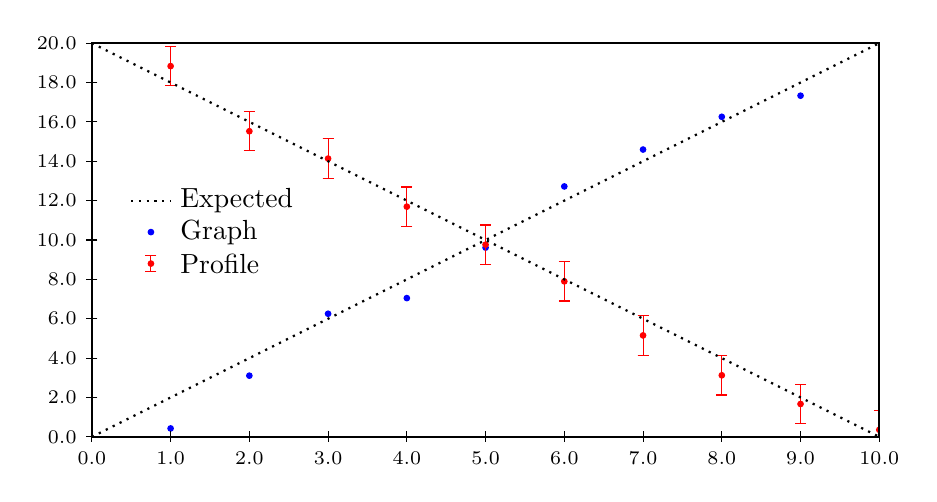
\begin{tikzpicture}
\begin{scope}[]
\clip (0,0) rectangle (10,5);
\draw[blue,fill=blue] (0.0,-0.11265896280989846) circle(1pt); 
\draw[blue,fill=blue] (1.0,0.1067177852637789) circle(1pt); 
\draw[blue,fill=blue] (2.0,0.7769855849859401) circle(1pt); 
\draw[blue,fill=blue] (3.0,1.563221741876979) circle(1pt); 
\draw[blue,fill=blue] (4.0,1.7617895415264044) circle(1pt); 
\draw[blue,fill=blue] (5.0,2.4034006696545265) circle(1pt); 
\draw[blue,fill=blue] (6.0,3.180089516667903) circle(1pt); 
\draw[blue,fill=blue] (7.0,3.648625789175461) circle(1pt); 
\draw[blue,fill=blue] (8.0,4.064206053390634) circle(1pt); 
\draw[blue,fill=blue] (9.0,4.332624590366722) circle(1pt); 
\draw[blue,fill=blue] (10.0,5.326777041467101) circle(1pt); 
\draw[draw=red,fill=red] (0.0,5.124148935749544) -- (0.0,5.624148935749544);
\draw[draw=red,fill=red] (0.0,5.374148935749544) circle(1pt); 
\draw[draw=red,fill=red] (0.0cm -2pt,5.124148935749544) -- (0.0cm + 2pt,5.124148935749544);
\draw[draw=red,fill=red] (0.0cm -2pt,5.624148935749544) -- (0.0cm + 2pt,5.624148935749544);
\draw[draw=red,fill=red] (1.0,4.457987941424418) -- (1.0,4.957987941424418);
\draw[draw=red,fill=red] (1.0,4.707987941424418) circle(1pt); 
\draw[draw=red,fill=red] (1.0cm -2pt,4.457987941424418) -- (1.0cm + 2pt,4.457987941424418);
\draw[draw=red,fill=red] (1.0cm -2pt,4.957987941424418) -- (1.0cm + 2pt,4.957987941424418);
\draw[draw=red,fill=red] (2.0,3.6309822345258023) -- (2.0,4.130982234525803);
\draw[draw=red,fill=red] (2.0,3.8809822345258023) circle(1pt); 
\draw[draw=red,fill=red] (2.0cm -2pt,3.6309822345258023) -- (2.0cm + 2pt,3.6309822345258023);
\draw[draw=red,fill=red] (2.0cm -2pt,4.130982234525803) -- (2.0cm + 2pt,4.130982234525803);
\draw[draw=red,fill=red] (3.0,3.283897225802921) -- (3.0,3.783897225802921);
\draw[draw=red,fill=red] (3.0,3.533897225802921) circle(1pt); 
\draw[draw=red,fill=red] (3.0cm -2pt,3.283897225802921) -- (3.0cm + 2pt,3.283897225802921);
\draw[draw=red,fill=red] (3.0cm -2pt,3.783897225802921) -- (3.0cm + 2pt,3.783897225802921);
\draw[draw=red,fill=red] (4.0,2.6732150073423946) -- (4.0,3.1732150073423946);
\draw[draw=red,fill=red] (4.0,2.9232150073423946) circle(1pt); 
\draw[draw=red,fill=red] (4.0cm -2pt,2.6732150073423946) -- (4.0cm + 2pt,2.6732150073423946);
\draw[draw=red,fill=red] (4.0cm -2pt,3.1732150073423946) -- (4.0cm + 2pt,3.1732150073423946);
\draw[draw=red,fill=red] (5.0,2.190451555285626) -- (5.0,2.690451555285626);
\draw[draw=red,fill=red] (5.0,2.440451555285626) circle(1pt); 
\draw[draw=red,fill=red] (5.0cm -2pt,2.190451555285626) -- (5.0cm + 2pt,2.190451555285626);
\draw[draw=red,fill=red] (5.0cm -2pt,2.690451555285626) -- (5.0cm + 2pt,2.690451555285626);
\draw[draw=red,fill=red] (6.0,1.7244627675920052) -- (6.0,2.224462767592005);
\draw[draw=red,fill=red] (6.0,1.9744627675920052) circle(1pt); 
\draw[draw=red,fill=red] (6.0cm -2pt,1.7244627675920052) -- (6.0cm + 2pt,1.7244627675920052);
\draw[draw=red,fill=red] (6.0cm -2pt,2.224462767592005) -- (6.0cm + 2pt,2.224462767592005);
\draw[draw=red,fill=red] (7.0,1.0380715044115072) -- (7.0,1.5380715044115072);
\draw[draw=red,fill=red] (7.0,1.2880715044115072) circle(1pt); 
\draw[draw=red,fill=red] (7.0cm -2pt,1.0380715044115072) -- (7.0cm + 2pt,1.0380715044115072);
\draw[draw=red,fill=red] (7.0cm -2pt,1.5380715044115072) -- (7.0cm + 2pt,1.5380715044115072);
\draw[draw=red,fill=red] (8.0,0.5317291768813934) -- (8.0,1.0317291768813934);
\draw[draw=red,fill=red] (8.0,0.7817291768813934) circle(1pt); 
\draw[draw=red,fill=red] (8.0cm -2pt,0.5317291768813934) -- (8.0cm + 2pt,0.5317291768813934);
\draw[draw=red,fill=red] (8.0cm -2pt,1.0317291768813934) -- (8.0cm + 2pt,1.0317291768813934);
\draw[draw=red,fill=red] (9.0,0.16715869395498462) -- (9.0,0.6671586939549846);
\draw[draw=red,fill=red] (9.0,0.4171586939549846) circle(1pt); 
\draw[draw=red,fill=red] (9.0cm -2pt,0.16715869395498462) -- (9.0cm + 2pt,0.16715869395498462);
\draw[draw=red,fill=red] (9.0cm -2pt,0.6671586939549846) -- (9.0cm + 2pt,0.6671586939549846);
\draw[draw=red,fill=red] (10.0,-0.16059765768477846) -- (10.0,0.33940234231522154);
\draw[draw=red,fill=red] (10.0,0.08940234231522154) circle(1pt); 
\draw[draw=red,fill=red] (10.0cm -2pt,-0.16059765768477846) -- (10.0cm + 2pt,-0.16059765768477846);
\draw[draw=red,fill=red] (10.0cm -2pt,0.33940234231522154) -- (10.0cm + 2pt,0.33940234231522154);
\draw[thick,dotted] (0.5,3.0) -- (1.0,3.0);
\node[right,] at (1.0,3.0) {Expected};
\draw[blue,fill=blue] (0.75,2.6) circle(1pt); 
\node[right,] at (1.0,2.6) {Graph};
\draw[red, fill=red] (0.75,2.1000001) -- (0.75,2.3);
\draw[red, fill=red] (0.75,2.2) circle(1pt); 
\draw[red, fill=red] (0.75cm -2pt,2.1000001) -- (0.75cm + 2pt,2.1000001);
\draw[red, fill=red] (0.75cm -2pt,2.3) -- (0.75cm + 2pt,2.3);
\node[right,] at (1.0,2.2) {Profile};
\end{scope}
\draw (0,0cm + 2pt) -- (0, 0cm -2pt) node[below] {\scriptsize{\num[round-mode=places,round-precision=1]{0}}};
\draw (1,0cm + 2pt) -- (1, 0cm -2pt) node[below] {\scriptsize{\num[round-mode=places,round-precision=1]{1}}};
\draw (2,0cm + 2pt) -- (2, 0cm -2pt) node[below] {\scriptsize{\num[round-mode=places,round-precision=1]{2}}};
\draw (3,0cm + 2pt) -- (3, 0cm -2pt) node[below] {\scriptsize{\num[round-mode=places,round-precision=1]{3}}};
\draw (4,0cm + 2pt) -- (4, 0cm -2pt) node[below] {\scriptsize{\num[round-mode=places,round-precision=1]{4}}};
\draw (5,0cm + 2pt) -- (5, 0cm -2pt) node[below] {\scriptsize{\num[round-mode=places,round-precision=1]{5}}};
\draw (6,0cm + 2pt) -- (6, 0cm -2pt) node[below] {\scriptsize{\num[round-mode=places,round-precision=1]{6}}};
\draw (7,0cm + 2pt) -- (7, 0cm -2pt) node[below] {\scriptsize{\num[round-mode=places,round-precision=1]{7}}};
\draw (8,0cm + 2pt) -- (8, 0cm -2pt) node[below] {\scriptsize{\num[round-mode=places,round-precision=1]{8}}};
\draw (9,0cm + 2pt) -- (9, 0cm -2pt) node[below] {\scriptsize{\num[round-mode=places,round-precision=1]{9}}};
\draw (10,0cm + 2pt) -- (10, 0cm -2pt) node[below] {\scriptsize{\num[round-mode=places,round-precision=1]{10}}};
\draw (0cm + 2pt,0.    ) -- (0cm-2pt,0.    ) node[left] {\scriptsize{\num[round-mode=places,round-precision=1]{0}}};
\draw (0cm + 2pt,0.5    ) -- (0cm-2pt,0.5    ) node[left] {\scriptsize{\num[round-mode=places,round-precision=1]{2}}};
\draw (0cm + 2pt,1.    ) -- (0cm-2pt,1.    ) node[left] {\scriptsize{\num[round-mode=places,round-precision=1]{4}}};
\draw (0cm + 2pt,1.5    ) -- (0cm-2pt,1.5    ) node[left] {\scriptsize{\num[round-mode=places,round-precision=1]{6}}};
\draw (0cm + 2pt,2.    ) -- (0cm-2pt,2.    ) node[left] {\scriptsize{\num[round-mode=places,round-precision=1]{8}}};
\draw (0cm + 2pt,2.5    ) -- (0cm-2pt,2.5    ) node[left] {\scriptsize{\num[round-mode=places,round-precision=1]{10}}};
\draw (0cm + 2pt,3.    ) -- (0cm-2pt,3.    ) node[left] {\scriptsize{\num[round-mode=places,round-precision=1]{12}}};
\draw (0cm + 2pt,3.5    ) -- (0cm-2pt,3.5    ) node[left] {\scriptsize{\num[round-mode=places,round-precision=1]{14}}};
\draw (0cm + 2pt,4.    ) -- (0cm-2pt,4.    ) node[left] {\scriptsize{\num[round-mode=places,round-precision=1]{16}}};
\draw (0cm + 2pt,4.5    ) -- (0cm-2pt,4.5    ) node[left] {\scriptsize{\num[round-mode=places,round-precision=1]{18}}};
\draw (0cm + 2pt,5.    ) -- (0cm-2pt,5.    ) node[left] {\scriptsize{\num[round-mode=places,round-precision=1]{20}}};
\draw[thick,dotted] (0.0,0.0) -- (10.0,5.0);
\draw[thick,dotted] (0.0,5.0) -- (10.0,0.0);
\draw[thick] (0,0) rectangle (10,5);
\end{tikzpicture}
%%% Local Variables: 
%%% mode: latex 
%%% TeX-master: "master" 
%%% End:


  \caption{Data points with and without errors}
\end{figure}

\begin{figure}[H]
  \centering
  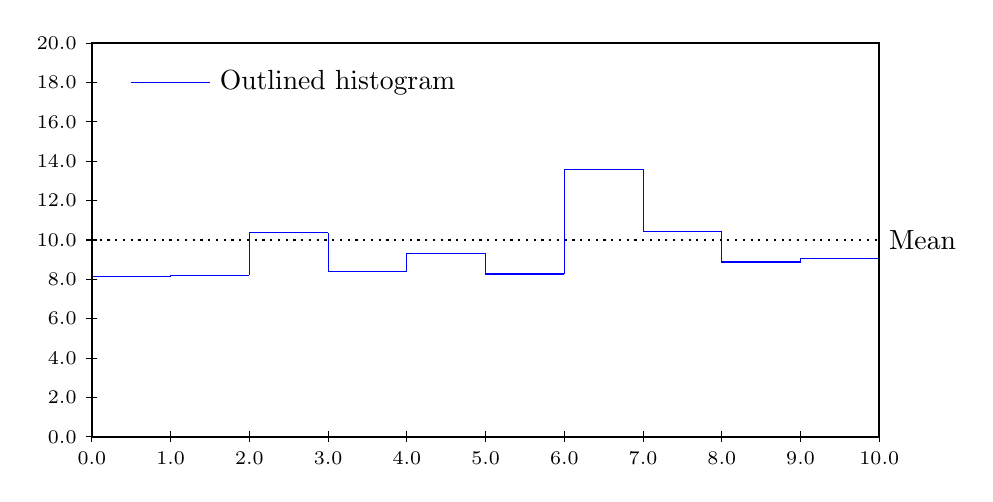
\begin{tikzpicture}
\begin{scope}[]
\clip (0,0) rectangle (10,5);
\begin{scope}[blue]
\draw[] (0.0,2.040753989729346) -- (1.0,2.040753989729346);
\draw (1.0,2.040753989729346) -- (1.0,2.0520371396851527) -- (2.0,2.0520371396851527);
\draw (2.0,2.0520371396851527) -- (2.0,2.589490136587087) -- (3.0,2.589490136587087);
\draw (3.0,2.589490136587087) -- (3.0,2.10531930397396) -- (4.0,2.10531930397396);
\draw (4.0,2.10531930397396) -- (4.0,2.328047479221825) -- (5.0,2.328047479221825);
\draw (5.0,2.328047479221825) -- (5.0,2.067390163042384) -- (6.0,2.067390163042384);
\draw (6.0,2.067390163042384) -- (6.0,3.3961419895360887) -- (7.0,3.3961419895360887);
\draw (7.0,3.3961419895360887) -- (7.0,2.6085288458106475) -- (8.0,2.6085288458106475);
\draw (8.0,2.6085288458106475) -- (8.0,2.2210174657245827) -- (9.0,2.2210174657245827);
\draw (9.0,2.2210174657245827) -- (9.0,2.2670683657782047) -- (10.0,2.2670683657782047);
\end{scope}
\end{scope}
\draw (0,0cm + 2pt) -- (0, 0cm -2pt) node[below] {\scriptsize{\num[round-mode=places,round-precision=1]{0}}};
\draw (1,0cm + 2pt) -- (1, 0cm -2pt) node[below] {\scriptsize{\num[round-mode=places,round-precision=1]{1}}};
\draw (2,0cm + 2pt) -- (2, 0cm -2pt) node[below] {\scriptsize{\num[round-mode=places,round-precision=1]{2}}};
\draw (3,0cm + 2pt) -- (3, 0cm -2pt) node[below] {\scriptsize{\num[round-mode=places,round-precision=1]{3}}};
\draw (4,0cm + 2pt) -- (4, 0cm -2pt) node[below] {\scriptsize{\num[round-mode=places,round-precision=1]{4}}};
\draw (5,0cm + 2pt) -- (5, 0cm -2pt) node[below] {\scriptsize{\num[round-mode=places,round-precision=1]{5}}};
\draw (6,0cm + 2pt) -- (6, 0cm -2pt) node[below] {\scriptsize{\num[round-mode=places,round-precision=1]{6}}};
\draw (7,0cm + 2pt) -- (7, 0cm -2pt) node[below] {\scriptsize{\num[round-mode=places,round-precision=1]{7}}};
\draw (8,0cm + 2pt) -- (8, 0cm -2pt) node[below] {\scriptsize{\num[round-mode=places,round-precision=1]{8}}};
\draw (9,0cm + 2pt) -- (9, 0cm -2pt) node[below] {\scriptsize{\num[round-mode=places,round-precision=1]{9}}};
\draw (10,0cm + 2pt) -- (10, 0cm -2pt) node[below] {\scriptsize{\num[round-mode=places,round-precision=1]{10}}};
\draw (0cm + 2pt,0.    ) -- (0cm-2pt,0.    ) node[left] {\scriptsize{\num[round-mode=places,round-precision=1]{0}}};
\draw (0cm + 2pt,0.5    ) -- (0cm-2pt,0.5    ) node[left] {\scriptsize{\num[round-mode=places,round-precision=1]{2}}};
\draw (0cm + 2pt,1.    ) -- (0cm-2pt,1.    ) node[left] {\scriptsize{\num[round-mode=places,round-precision=1]{4}}};
\draw (0cm + 2pt,1.5    ) -- (0cm-2pt,1.5    ) node[left] {\scriptsize{\num[round-mode=places,round-precision=1]{6}}};
\draw (0cm + 2pt,2.    ) -- (0cm-2pt,2.    ) node[left] {\scriptsize{\num[round-mode=places,round-precision=1]{8}}};
\draw (0cm + 2pt,2.5    ) -- (0cm-2pt,2.5    ) node[left] {\scriptsize{\num[round-mode=places,round-precision=1]{10}}};
\draw (0cm + 2pt,3.    ) -- (0cm-2pt,3.    ) node[left] {\scriptsize{\num[round-mode=places,round-precision=1]{12}}};
\draw (0cm + 2pt,3.5    ) -- (0cm-2pt,3.5    ) node[left] {\scriptsize{\num[round-mode=places,round-precision=1]{14}}};
\draw (0cm + 2pt,4.    ) -- (0cm-2pt,4.    ) node[left] {\scriptsize{\num[round-mode=places,round-precision=1]{16}}};
\draw (0cm + 2pt,4.5    ) -- (0cm-2pt,4.5    ) node[left] {\scriptsize{\num[round-mode=places,round-precision=1]{18}}};
\draw (0cm + 2pt,5.    ) -- (0cm-2pt,5.    ) node[left] {\scriptsize{\num[round-mode=places,round-precision=1]{20}}};
\draw[thick] (0,0) rectangle (10,5);
\draw[thick,dotted] (0.0,2.5) -- (10.0,2.5);
\node[right] at (10.0,2.5) {Mean};
\draw[blue] (0.5,4.5) -- (1.5,4.5);
\node[right,] at (1.5,4.5) {Outlined histogram};
\end{tikzpicture}
%%% Local Variables: 
%%% mode: latex 
%%% TeX-master: "master" 
%%% End:


  \caption{Basic histogram}
\end{figure}

\begin{figure}[H]
  \centering
  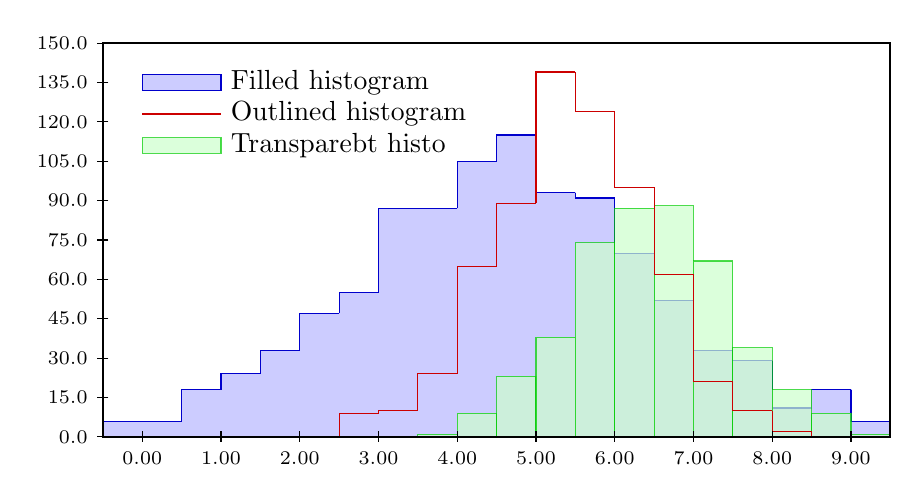
\begin{tikzpicture}
\begin{scope}[]
\clip (0,0) rectangle (10,5);
\begin{scope}[draw=blue!20,fill=blue!20]
\filldraw[] (0.0,0.0) -- (0.0,0.2) -- (0.5,0.2) -- (0.5,0.0);
\filldraw[] (0.5,0.0) -- (0.5,0.2) -- (1.0,0.2) -- (1.0,0.0);
\filldraw[] (1.0,0.0) -- (1.0,0.6) -- (1.5,0.6) -- (1.5,0.0);
\filldraw[] (1.5,0.0) -- (1.5,0.8) -- (2.0,0.8) -- (2.0,0.0);
\filldraw[] (2.0,0.0) -- (2.0,1.1) -- (2.5,1.1) -- (2.5,0.0);
\filldraw[] (2.5,0.0) -- (2.5,1.5666667) -- (3.0,1.5666667) -- (3.0,0.0);
\filldraw[] (3.0,0.0) -- (3.0,1.8333334) -- (3.5,1.8333334) -- (3.5,0.0);
\filldraw[] (3.5,0.0) -- (3.5,2.9) -- (4.0,2.9) -- (4.0,0.0);
\filldraw[] (4.0,0.0) -- (4.0,2.9) -- (4.5,2.9) -- (4.5,0.0);
\filldraw[] (4.5,0.0) -- (4.5,3.5) -- (5.0,3.5) -- (5.0,0.0);
\filldraw[] (5.0,0.0) -- (5.0,3.8333333) -- (5.5,3.8333333) -- (5.5,0.0);
\filldraw[] (5.5,0.0) -- (5.5,3.1) -- (6.0,3.1) -- (6.0,0.0);
\filldraw[] (6.0,0.0) -- (6.0,3.0333333) -- (6.5,3.0333333) -- (6.5,0.0);
\filldraw[] (6.5,0.0) -- (6.5,2.3333333) -- (7.0,2.3333333) -- (7.0,0.0);
\filldraw[] (7.0,0.0) -- (7.0,1.7333333) -- (7.5,1.7333333) -- (7.5,0.0);
\filldraw[] (7.5,0.0) -- (7.5,1.1) -- (8.0,1.1) -- (8.0,0.0);
\filldraw[] (8.0,0.0) -- (8.0,0.96666664) -- (8.5,0.96666664) -- (8.5,0.0);
\filldraw[] (8.5,0.0) -- (8.5,0.36666667) -- (9.0,0.36666667) -- (9.0,0.0);
\filldraw[] (9.0,0.0) -- (9.0,0.6) -- (9.5,0.6) -- (9.5,0.0);
\filldraw[] (9.5,0.0) -- (9.5,0.2) -- (10.0,0.2) -- (10.0,0.0);
\end{scope}
\begin{scope}[blue!80!black]
\draw[] (0.0,0.2) -- (0.5,0.2);
\draw (0.5,0.2) -- (0.5,0.2) -- (1.0,0.2);
\draw (1.0,0.2) -- (1.0,0.6) -- (1.5,0.6);
\draw (1.5,0.6) -- (1.5,0.8) -- (2.0,0.8);
\draw (2.0,0.8) -- (2.0,1.1) -- (2.5,1.1);
\draw (2.5,1.1) -- (2.5,1.5666667) -- (3.0,1.5666667);
\draw (3.0,1.5666667) -- (3.0,1.8333334) -- (3.5,1.8333334);
\draw (3.5,1.8333334) -- (3.5,2.9) -- (4.0,2.9);
\draw (4.0,2.9) -- (4.0,2.9) -- (4.5,2.9);
\draw (4.5,2.9) -- (4.5,3.5) -- (5.0,3.5);
\draw (5.0,3.5) -- (5.0,3.8333333) -- (5.5,3.8333333);
\draw (5.5,3.8333333) -- (5.5,3.1) -- (6.0,3.1);
\draw (6.0,3.1) -- (6.0,3.0333333) -- (6.5,3.0333333);
\draw (6.5,3.0333333) -- (6.5,2.3333333) -- (7.0,2.3333333);
\draw (7.0,2.3333333) -- (7.0,1.7333333) -- (7.5,1.7333333);
\draw (7.5,1.7333333) -- (7.5,1.1) -- (8.0,1.1);
\draw (8.0,1.1) -- (8.0,0.96666664) -- (8.5,0.96666664);
\draw (8.5,0.96666664) -- (8.5,0.36666667) -- (9.0,0.36666667);
\draw (9.0,0.36666667) -- (9.0,0.6) -- (9.5,0.6);
\draw (9.5,0.6) -- (9.5,0.2) -- (10.0,0.2);
\end{scope}
\begin{scope}[opacity=0.7,draw=green!80!black,fill=green!20]
\filldraw[] (0.0,0.0) -- (0.0,0.0) -- (0.5,0.0) -- (0.5,0.0);
\filldraw[] (0.5,0.0) -- (0.5,0.0) -- (1.0,0.0) -- (1.0,0.0);
\filldraw[] (1.0,0.0) -- (1.0,0.0) -- (1.5,0.0) -- (1.5,0.0);
\filldraw[] (1.5,0.0) -- (1.5,0.0) -- (2.0,0.0) -- (2.0,0.0);
\filldraw[] (2.0,0.0) -- (2.0,0.0) -- (2.5,0.0) -- (2.5,0.0);
\filldraw[] (2.5,0.0) -- (2.5,0.0) -- (3.0,0.0) -- (3.0,0.0);
\filldraw[] (3.0,0.0) -- (3.0,0.0) -- (3.5,0.0) -- (3.5,0.0);
\filldraw[] (3.5,0.0) -- (3.5,0.0) -- (4.0,0.0) -- (4.0,0.0);
\filldraw[] (4.0,0.0) -- (4.0,0.033333335) -- (4.5,0.033333335) -- (4.5,0.0);
\filldraw[] (4.5,0.0) -- (4.5,0.3) -- (5.0,0.3) -- (5.0,0.0);
\filldraw[] (5.0,0.0) -- (5.0,0.76666665) -- (5.5,0.76666665) -- (5.5,0.0);
\filldraw[] (5.5,0.0) -- (5.5,1.2666667) -- (6.0,1.2666667) -- (6.0,0.0);
\filldraw[] (6.0,0.0) -- (6.0,2.4666667) -- (6.5,2.4666667) -- (6.5,0.0);
\filldraw[] (6.5,0.0) -- (6.5,2.9) -- (7.0,2.9) -- (7.0,0.0);
\filldraw[] (7.0,0.0) -- (7.0,2.9333334) -- (7.5,2.9333334) -- (7.5,0.0);
\filldraw[] (7.5,0.0) -- (7.5,2.2333333) -- (8.0,2.2333333) -- (8.0,0.0);
\filldraw[] (8.0,0.0) -- (8.0,1.1333333) -- (8.5,1.1333333) -- (8.5,0.0);
\filldraw[] (8.5,0.0) -- (8.5,0.6) -- (9.0,0.6) -- (9.0,0.0);
\filldraw[] (9.0,0.0) -- (9.0,0.3) -- (9.5,0.3) -- (9.5,0.0);
\filldraw[] (9.5,0.0) -- (9.5,0.033333335) -- (10.0,0.033333335) -- (10.0,0.0);
\end{scope}
\begin{scope}[red!80!black]
\draw[] (0.0,0.0) -- (0.5,0.0);
\draw (0.5,0.0) -- (0.5,0.0) -- (1.0,0.0);
\draw (1.0,0.0) -- (1.0,0.0) -- (1.5,0.0);
\draw (1.5,0.0) -- (1.5,0.0) -- (2.0,0.0);
\draw (2.0,0.0) -- (2.0,0.0) -- (2.5,0.0);
\draw (2.5,0.0) -- (2.5,0.0) -- (3.0,0.0);
\draw (3.0,0.0) -- (3.0,0.3) -- (3.5,0.3);
\draw (3.5,0.3) -- (3.5,0.33333334) -- (4.0,0.33333334);
\draw (4.0,0.33333334) -- (4.0,0.8) -- (4.5,0.8);
\draw (4.5,0.8) -- (4.5,2.1666667) -- (5.0,2.1666667);
\draw (5.0,2.1666667) -- (5.0,2.9666667) -- (5.5,2.9666667);
\draw (5.5,2.9666667) -- (5.5,4.633333) -- (6.0,4.633333);
\draw (6.0,4.633333) -- (6.0,4.133333) -- (6.5,4.133333);
\draw (6.5,4.133333) -- (6.5,3.1666667) -- (7.0,3.1666667);
\draw (7.0,3.1666667) -- (7.0,2.0666666) -- (7.5,2.0666666);
\draw (7.5,2.0666666) -- (7.5,0.7) -- (8.0,0.7);
\draw (8.0,0.7) -- (8.0,0.33333334) -- (8.5,0.33333334);
\draw (8.5,0.33333334) -- (8.5,0.06666667) -- (9.0,0.06666667);
\draw (9.0,0.06666667) -- (9.0,0.0) -- (9.5,0.0);
\draw (9.5,0.0) -- (9.5,0.0) -- (10.0,0.0);
\end{scope}
\end{scope}
\draw (0.5,0cm + 2pt) -- (0.5, 0cm -2pt) node[below] {\scriptsize{\num[round-mode=places,round-precision=2]{0}}};
\draw (1.5,0cm + 2pt) -- (1.5, 0cm -2pt) node[below] {\scriptsize{\num[round-mode=places,round-precision=2]{1}}};
\draw (2.5,0cm + 2pt) -- (2.5, 0cm -2pt) node[below] {\scriptsize{\num[round-mode=places,round-precision=2]{2}}};
\draw (3.5,0cm + 2pt) -- (3.5, 0cm -2pt) node[below] {\scriptsize{\num[round-mode=places,round-precision=2]{3}}};
\draw (4.5,0cm + 2pt) -- (4.5, 0cm -2pt) node[below] {\scriptsize{\num[round-mode=places,round-precision=2]{4}}};
\draw (5.5,0cm + 2pt) -- (5.5, 0cm -2pt) node[below] {\scriptsize{\num[round-mode=places,round-precision=2]{5}}};
\draw (6.5,0cm + 2pt) -- (6.5, 0cm -2pt) node[below] {\scriptsize{\num[round-mode=places,round-precision=2]{6}}};
\draw (7.5,0cm + 2pt) -- (7.5, 0cm -2pt) node[below] {\scriptsize{\num[round-mode=places,round-precision=2]{7}}};
\draw (8.5,0cm + 2pt) -- (8.5, 0cm -2pt) node[below] {\scriptsize{\num[round-mode=places,round-precision=2]{8}}};
\draw (9.5,0cm + 2pt) -- (9.5, 0cm -2pt) node[below] {\scriptsize{\num[round-mode=places,round-precision=2]{9}}};
\draw (0cm + 2pt,0.    ) -- (0cm-2pt,0.    ) node[left] {\scriptsize{\num[round-mode=places,round-precision=1]{0}}};
\draw (0cm + 2pt,0.5    ) -- (0cm-2pt,0.5    ) node[left] {\scriptsize{\num[round-mode=places,round-precision=1]{15}}};
\draw (0cm + 2pt,1.    ) -- (0cm-2pt,1.    ) node[left] {\scriptsize{\num[round-mode=places,round-precision=1]{30}}};
\draw (0cm + 2pt,1.5    ) -- (0cm-2pt,1.5    ) node[left] {\scriptsize{\num[round-mode=places,round-precision=1]{45}}};
\draw (0cm + 2pt,2.    ) -- (0cm-2pt,2.    ) node[left] {\scriptsize{\num[round-mode=places,round-precision=1]{60}}};
\draw (0cm + 2pt,2.5    ) -- (0cm-2pt,2.5    ) node[left] {\scriptsize{\num[round-mode=places,round-precision=1]{75}}};
\draw (0cm + 2pt,3.    ) -- (0cm-2pt,3.    ) node[left] {\scriptsize{\num[round-mode=places,round-precision=1]{90}}};
\draw (0cm + 2pt,3.5    ) -- (0cm-2pt,3.5    ) node[left] {\scriptsize{\num[round-mode=places,round-precision=1]{105}}};
\draw (0cm + 2pt,4.    ) -- (0cm-2pt,4.    ) node[left] {\scriptsize{\num[round-mode=places,round-precision=1]{120}}};
\draw (0cm + 2pt,4.5    ) -- (0cm-2pt,4.5    ) node[left] {\scriptsize{\num[round-mode=places,round-precision=1]{135}}};
\draw (0cm + 2pt,5.    ) -- (0cm-2pt,5.    ) node[left] {\scriptsize{\num[round-mode=places,round-precision=1]{150}}};
\draw[thick] (0,0) rectangle (10,5);
\draw[draw=blue!20,fill=blue!20] (0.5,4.4) rectangle (1.5,4.6);
; 
\draw[blue!80!black] (0.5,4.4) rectangle (1.5,4.6);
; 
\node[right,] at (1.5,4.5) {Filled histogram};
\draw[red!80!black] (0.5,4.1) -- (1.5,4.1);
\node[right,] at (1.5,4.1) {Outlined histogram};
\draw[opacity=0.7,draw=green!80!black,fill=green!20] (0.5,3.6000001) rectangle (1.5,3.8);
; 
\node[right,] at (1.5,3.7) {Transparebt histo};
\end{tikzpicture}
%%% Local Variables: 
%%% mode: latex 
%%% TeX-master: "master" 
%%% End:


  \caption{Two histograms in the same figure}
\end{figure}

\section{Fitting with Levenberg marquart algorithm}
\label{sec:LMA}

\begin{figure}[H]
  \centering
  \documentclass{standalone}
\ifx\HCode\UnDef\else\def\pgfsysdriver{pgfsys-tex4ht.def}\fi
\usepackage{tikz}
\usepackage{color}
\usepackage{siunitx}
\usetikzlibrary{arrows,shapes}
\begin{document}
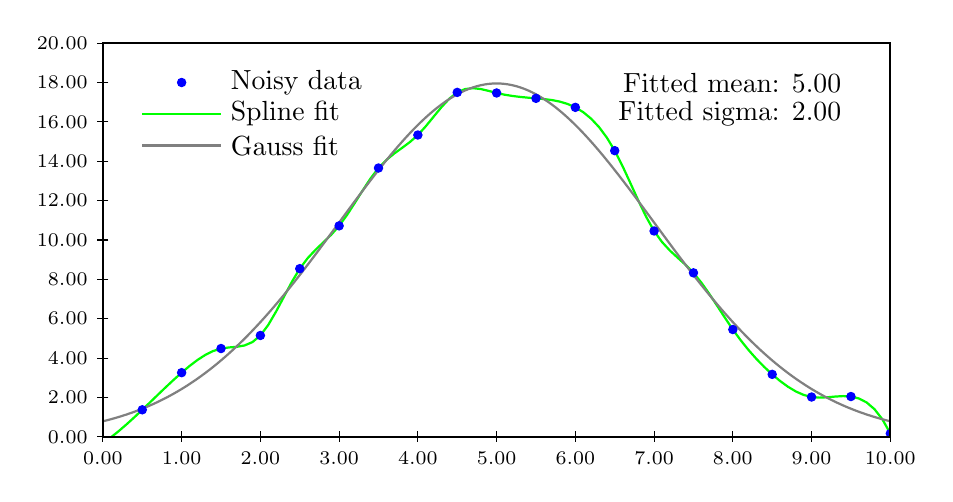
\begin{tikzpicture}
\begin{scope}[]
\pgfpathmoveto{ \pgfpointxy {0.0} {0.0}}
\pgfpathlineto{ \pgfpointxy {10.0} {0.0}}
\pgfpathlineto{ \pgfpointxy {10.0} {5.0}}
\pgfpathlineto{ \pgfpointxy {0.0} {5.0}}
\pgfpathclose
\pgfusepath{  clip, }
\begin{scope}[shift={(0.0,0.0)}]
\pgfsetxvec{\pgfpoint{1.0cm}{0cm}}
\pgfsetyvec{\pgfpoint{0cm}{0.25cm}}
\begin{scope}[shift={(0.0,0.0)}]
\begin{scope}[green,thick]
\pgfpathmoveto{ \pgfpointxy {0.0} {-0.3220822684578466}}
\pgfpathlineto{ \pgfpointxy {0.1} {-0.03179540914739956}}
\pgfpathlineto{ \pgfpointxy {0.2} {0.2885428151650948}}
\pgfpathlineto{ \pgfpointxy {0.3} {0.633328152486329}}
\pgfpathlineto{ \pgfpointxy {0.4} {0.9969563508229966}}
\pgfpathlineto{ \pgfpointxy {0.5} {1.3738231581817897}}
\pgfpathlineto{ \pgfpointxy {0.6} {1.7583243225694014}}
\pgfpathlineto{ \pgfpointxy {0.7} {2.144855591992525}}
\pgfpathlineto{ \pgfpointxy {0.8} {2.5278127144578533}}
\pgfpathlineto{ \pgfpointxy {0.9} {2.9015914379720784}}
\pgfpathlineto{ \pgfpointxy {1.0} {3.2605875105418933}}
\pgfpathlineto{ \pgfpointxy {1.1} {3.59798429165626}}
\pgfpathlineto{ \pgfpointxy {1.2} {3.9021155867332062}}
\pgfpathlineto{ \pgfpointxy {1.3} {4.160102812673034}}
\pgfpathlineto{ \pgfpointxy {1.4} {4.359067386376038}}
\pgfpathlineto{ \pgfpointxy {1.5} {4.486130724742518}}
\pgfpathlineto{ \pgfpointxy {1.6} {4.540874002276166}}
\pgfpathlineto{ \pgfpointxy {1.7} {4.572717423894254}}
\pgfpathlineto{ \pgfpointxy {1.8} {4.6435409521174424}}
\pgfpathlineto{ \pgfpointxy {1.9} {4.815224549466396}}
\pgfpathlineto{ \pgfpointxy {2.0} {5.149648178461778}}
\pgfpathlineto{ \pgfpointxy {2.1} {5.685601299272113}}
\pgfpathlineto{ \pgfpointxy {2.2} {6.3695113626573665}}
\pgfpathlineto{ \pgfpointxy {2.3} {7.124715317025358}}
\pgfpathlineto{ \pgfpointxy {2.4} {7.874550110783923}}
\pgfpathlineto{ \pgfpointxy {2.5} {8.54235269234088}}
\pgfpathlineto{ \pgfpointxy {2.6} {9.073464969531473}}
\pgfpathlineto{ \pgfpointxy {2.7} {9.50124868790061}}
\pgfpathlineto{ \pgfpointxy {2.8} {9.88107055242061}}
\pgfpathlineto{ \pgfpointxy {2.9} {10.268297268063803}}
\pgfpathlineto{ \pgfpointxy {3.0} {10.718295539802511}}
\pgfpathlineto{ \pgfpointxy {3.1} {11.268900377785958}}
\pgfpathlineto{ \pgfpointxy {3.2} {11.887820012870971}}
\pgfpathlineto{ \pgfpointxy {3.3} {12.52523098109127}}
\pgfpathlineto{ \pgfpointxy {3.4} {13.131309818480585}}
\pgfpathlineto{ \pgfpointxy {3.5} {13.656233061072639}}
\pgfpathlineto{ \pgfpointxy {3.6} {14.066283096326574}}
\pgfpathlineto{ \pgfpointxy {3.7} {14.392165717403207}}
\pgfpathlineto{ \pgfpointxy {3.8} {14.680692568888766}}
\pgfpathlineto{ \pgfpointxy {3.9} {14.978675295369484}}
\pgfpathlineto{ \pgfpointxy {4.0} {15.3329255414316}}
\pgfpathlineto{ \pgfpointxy {4.1} {15.773545607044694}}
\pgfpathlineto{ \pgfpointxy {4.2} {16.263800413711795}}
\pgfpathlineto{ \pgfpointxy {4.3} {16.75024553831928}}
\pgfpathlineto{ \pgfpointxy {4.4} {17.179436557753533}}
\pgfpathlineto{ \pgfpointxy {4.5} {17.497929048900925}}
\pgfpathlineto{ \pgfpointxy {4.6} {17.667544878429773}}
\pgfpathlineto{ \pgfpointxy {4.7} {17.711171072136075}}
\pgfpathlineto{ \pgfpointxy {4.8} {17.666960945597783}}
\pgfpathlineto{ \pgfpointxy {4.9} {17.57306781439283}}
\pgfpathlineto{ \pgfpointxy {5.0} {17.46764499409915}}
\pgfpathlineto{ \pgfpointxy {5.1} {17.38158457781227}}
\pgfpathlineto{ \pgfpointxy {5.2} {17.31673376869809}}
\pgfpathlineto{ \pgfpointxy {5.3} {17.267678547440084}}
\pgfpathlineto{ \pgfpointxy {5.4} {17.22900489472175}}
\pgfpathlineto{ \pgfpointxy {5.5} {17.195298791226566}}
\pgfpathlineto{ \pgfpointxy {5.6} {17.15975016321322}}
\pgfpathlineto{ \pgfpointxy {5.7} {17.109964719241223}}
\pgfpathlineto{ \pgfpointxy {5.8} {17.0321521134453}}
\pgfpathlineto{ \pgfpointxy {5.9} {16.912521999960166}}
\pgfpathlineto{ \pgfpointxy {6.0} {16.73728403292054}}
\pgfpathlineto{ \pgfpointxy {6.1} {16.492593096437812}}
\pgfpathlineto{ \pgfpointxy {6.2} {16.164384994530018}}
\pgfpathlineto{ \pgfpointxy {6.3} {15.738540761191885}}
\pgfpathlineto{ \pgfpointxy {6.4} {15.200941430418121}}
\pgfpathlineto{ \pgfpointxy {6.5} {14.537468036203448}}
\pgfpathlineto{ \pgfpointxy {6.6} {13.746955063475587}}
\pgfpathlineto{ \pgfpointxy {6.7} {12.880050800894296}}
\pgfpathlineto{ \pgfpointxy {6.8} {12.000356988052364}}
\pgfpathlineto{ \pgfpointxy {6.9} {11.171475364542555}}
\pgfpathlineto{ \pgfpointxy {7.0} {10.457007669957658}}
\pgfpathlineto{ \pgfpointxy {7.1} {9.900588706936261}}
\pgfpathlineto{ \pgfpointxy {7.2} {9.465985530300243}}
\pgfpathlineto{ \pgfpointxy {7.3} {9.096998257917303}}
\pgfpathlineto{ \pgfpointxy {7.4} {8.737427007655137}}
\pgfpathlineto{ \pgfpointxy {7.5} {8.331071897381452}}
\pgfpathlineto{ \pgfpointxy {7.6} {7.836306153830907}}
\pgfpathlineto{ \pgfpointxy {7.7} {7.269795439206012}}
\pgfpathlineto{ \pgfpointxy {7.8} {6.662778524576263}}
\pgfpathlineto{ \pgfpointxy {7.9} {6.046494181011129}}
\pgfpathlineto{ \pgfpointxy {8.0} {5.452181179580102}}
\pgfpathlineto{ \pgfpointxy {8.1} {4.905237179264141}}
\pgfpathlineto{ \pgfpointxy {8.2} {4.4076953906901215}}
\pgfpathlineto{ \pgfpointxy {8.3} {3.9557479123963915}}
\pgfpathlineto{ \pgfpointxy {8.4} {3.545586842921326}}
\pgfpathlineto{ \pgfpointxy {8.5} {3.173404280803272}}
\pgfpathlineto{ \pgfpointxy {8.6} {2.837587185462304}}
\pgfpathlineto{ \pgfpointxy {8.7} {2.545301959845368}}
\pgfpathlineto{ \pgfpointxy {8.8} {2.305909867781125}}
\pgfpathlineto{ \pgfpointxy {8.9} {2.128772173098246}}
\pgfpathlineto{ \pgfpointxy {9.0} {2.0232501396253917}}
\pgfpathlineto{ \pgfpointxy {9.1} {1.9919084111773382}}
\pgfpathlineto{ \pgfpointxy {9.2} {2.010125151513315}}
\pgfpathlineto{ \pgfpointxy {9.3} {2.046481904378665}}
\pgfpathlineto{ \pgfpointxy {9.4} {2.0695602135187294}}
\pgfpathlineto{ \pgfpointxy {9.5} {2.047941622678851}}
\pgfpathlineto{ \pgfpointxy {9.6} {1.9502076756043718}}
\pgfpathlineto{ \pgfpointxy {9.7} {1.744939916040635}}
\pgfpathlineto{ \pgfpointxy {9.8} {1.400719887732975}}
\pgfpathlineto{ \pgfpointxy {9.9} {0.8861291344267457}}
\pgfpathlineto{ \pgfpointxy {10.0} {0.16974919986728543}}
\pgfusepath{ stroke, }
\end{scope}
\begin{scope}[thick,gray]
\pgfpathmoveto{ \pgfpointxy {0.0} {0.7887735222102034}}
\pgfpathlineto{ \pgfpointxy {0.05} {0.8393826956517481}}
\pgfpathlineto{ \pgfpointxy {0.1} {0.892680947630374}}
\pgfpathlineto{ \pgfpointxy {0.15} {0.9487703099544526}}
\pgfpathlineto{ \pgfpointxy {0.2} {1.0077538632674794}}
\pgfpathlineto{ \pgfpointxy {0.25} {1.0697355373456514}}
\pgfpathlineto{ \pgfpointxy {0.3} {1.134819896183258}}
\pgfpathlineto{ \pgfpointxy {0.35} {1.203111907750662}}
\pgfpathlineto{ \pgfpointxy {0.4} {1.2747166983715252}}
\pgfpathlineto{ \pgfpointxy {0.45} {1.3497392917319906}}
\pgfpathlineto{ \pgfpointxy {0.5} {1.4282843326044656}}
\pgfpathlineto{ \pgfpointxy {0.55} {1.5104557954424003}}
\pgfpathlineto{ \pgfpointxy {0.6} {1.5963566780798044}}
\pgfpathlineto{ \pgfpointxy {0.65} {1.6860886808498898}}
\pgfpathlineto{ \pgfpointxy {0.7} {1.779751871521008}}
\pgfpathlineto{ \pgfpointxy {0.75} {1.8774443365345639}}
\pgfpathlineto{ \pgfpointxy {0.8} {1.9792618191185283}}
\pgfpathlineto{ \pgfpointxy {0.85} {2.0852973449411976}}
\pgfpathlineto{ \pgfpointxy {0.9} {2.1956408360624864}}
\pgfpathlineto{ \pgfpointxy {0.95} {2.310378714033865}}
\pgfpathlineto{ \pgfpointxy {1.0} {2.42959349309268}}
\pgfpathlineto{ \pgfpointxy {1.05} {2.5533633644912777}}
\pgfpathlineto{ \pgfpointxy {1.1} {2.6817617730958987}}
\pgfpathlineto{ \pgfpointxy {1.15} {2.8148569874838527}}
\pgfpathlineto{ \pgfpointxy {1.2} {2.95271166485958}}
\pgfpathlineto{ \pgfpointxy {1.25} {3.0953824122002476}}
\pgfpathlineto{ \pgfpointxy {1.3} {3.2429193451289016}}
\pgfpathlineto{ \pgfpointxy {1.35} {3.3953656460971313}}
\pgfpathlineto{ \pgfpointxy {1.4} {3.5527571235392896}}
\pgfpathlineto{ \pgfpointxy {1.45} {3.7151217737356554}}
\pgfpathlineto{ \pgfpointxy {1.5} {3.882479347192031}}
\pgfpathlineto{ \pgfpointxy {1.55} {4.0548409214074095}}
\pgfpathlineto{ \pgfpointxy {1.6} {4.232208481958889}}
\pgfpathlineto{ \pgfpointxy {1.65} {4.414574513883361}}
\pgfpathlineto{ \pgfpointxy {1.7} {4.601921605377953}}
\pgfpathlineto{ \pgfpointxy {1.75} {4.794222065875254}}
\pgfpathlineto{ \pgfpointxy {1.8} {4.991437560574411}}
\pgfpathlineto{ \pgfpointxy {1.85} {5.193518763524646}}
\pgfpathlineto{ \pgfpointxy {1.9} {5.400405031363236}}
\pgfpathlineto{ \pgfpointxy {1.95} {5.612024099804946}}
\pgfpathlineto{ \pgfpointxy {2.0} {5.828291804963986}}
\pgfpathlineto{ \pgfpointxy {2.05} {6.0491118315624055}}
\pgfpathlineto{ \pgfpointxy {2.1} {6.27437549004005}}
\pgfpathlineto{ \pgfpointxy {2.15} {6.503961524530807}}
\pgfpathlineto{ \pgfpointxy {2.2} {6.7377359536073405}}
\pgfpathlineto{ \pgfpointxy {2.25} {6.975551945622008}}
\pgfpathlineto{ \pgfpointxy {2.3} {7.217249730385189}}
\pgfpathlineto{ \pgfpointxy {2.35} {7.462656548823516}}
\pgfpathlineto{ \pgfpointxy {2.4} {7.71158664215013}}
\pgfpathlineto{ \pgfpointxy {2.45} {7.963841281956886}}
\pgfpathlineto{ \pgfpointxy {2.5} {8.219208842504782}}
\pgfpathlineto{ \pgfpointxy {2.55} {8.47746491634448}}
\pgfpathlineto{ \pgfpointxy {2.6} {8.73837247424338}}
\pgfpathlineto{ \pgfpointxy {2.65} {9.001682070230748}}
\pgfpathlineto{ \pgfpointxy {2.7} {9.267132092397667}}
\pgfpathlineto{ \pgfpointxy {2.75} {9.534449059905283}}
\pgfpathlineto{ \pgfpointxy {2.8} {9.803347966463585}}
\pgfpathlineto{ \pgfpointxy {2.85} {10.073532670344598}}
\pgfpathlineto{ \pgfpointxy {2.9} {10.344696330789311}}
\pgfpathlineto{ \pgfpointxy {2.95} {10.6165218904581}}
\pgfpathlineto{ \pgfpointxy {3.0} {10.888682603360296}}
\pgfpathlineto{ \pgfpointxy {3.05} {11.160842607482026}}
\pgfpathlineto{ \pgfpointxy {3.1} {11.432657541112373}}
\pgfpathlineto{ \pgfpointxy {3.15} {11.703775201648687}}
\pgfpathlineto{ \pgfpointxy {3.2} {11.973836245442861}}
\pgfpathlineto{ \pgfpointxy {3.25} {12.242474927033365}}
\pgfpathlineto{ \pgfpointxy {3.3} {12.509319875893764}}
\pgfpathlineto{ \pgfpointxy {3.35} {12.773994908618867}}
\pgfpathlineto{ \pgfpointxy {3.4} {13.036119874265678}}
\pgfpathlineto{ \pgfpointxy {3.45} {13.295311530369304}}
\pgfpathlineto{ \pgfpointxy {3.5} {13.551184446965188}}
\pgfpathlineto{ \pgfpointxy {3.55} {13.803351935769804}}
\pgfpathlineto{ \pgfpointxy {3.6} {14.051427001503281}}
\pgfpathlineto{ \pgfpointxy {3.65} {14.295023312180714}}
\pgfpathlineto{ \pgfpointxy {3.7} {14.533756185055205}}
\pgfpathlineto{ \pgfpointxy {3.75} {14.767243584765959}}
\pgfpathlineto{ \pgfpointxy {3.8} {14.995107130130082}}
\pgfpathlineto{ \pgfpointxy {3.85} {15.216973105918132}}
\pgfpathlineto{ \pgfpointxy {3.9} {15.432473475871411}}
\pgfpathlineto{ \pgfpointxy {3.95} {15.64124689315482}}
\pgfpathlineto{ \pgfpointxy {4.0} {15.84293970439265}}
\pgfpathlineto{ \pgfpointxy {4.05} {16.037206943407437}}
\pgfpathlineto{ \pgfpointxy {4.1} {16.223713310773366}}
\pgfpathlineto{ \pgfpointxy {4.15} {16.40213413530702}}
\pgfpathlineto{ \pgfpointxy {4.2} {16.572156313648794}}
\pgfpathlineto{ \pgfpointxy {4.25} {16.73347922413886}}
\pgfpathlineto{ \pgfpointxy {4.3} {16.885815611261478}}
\pgfpathlineto{ \pgfpointxy {4.35} {17.028892437021163}}
\pgfpathlineto{ \pgfpointxy {4.4} {17.162451695722886}}
\pgfpathlineto{ \pgfpointxy {4.45} {17.28625118875603}}
\pgfpathlineto{ \pgfpointxy {4.5} {17.40006525612754}}
\pgfpathlineto{ \pgfpointxy {4.55} {17.503685461653063}}
\pgfpathlineto{ \pgfpointxy {4.6} {17.596921228894864}}
\pgfpathlineto{ \pgfpointxy {4.65} {17.679600425131426}}
\pgfpathlineto{ \pgfpointxy {4.7} {17.751569890854366}}
\pgfpathlineto{ \pgfpointxy {4.75} {17.8126959125131}}
\pgfpathlineto{ \pgfpointxy {4.8} {17.862864636464906}}
\pgfpathlineto{ \pgfpointxy {4.85} {17.90198242233675}}
\pgfpathlineto{ \pgfpointxy {4.9} {17.929976134263764}}
\pgfpathlineto{ \pgfpointxy {4.95} {17.946793368736568}}
\pgfpathlineto{ \pgfpointxy {5.0} {17.952402618063857}}
\pgfpathlineto{ \pgfpointxy {5.05} {17.946793368736568}}
\pgfpathlineto{ \pgfpointxy {5.1} {17.929976134263764}}
\pgfpathlineto{ \pgfpointxy {5.15} {17.90198242233675}}
\pgfpathlineto{ \pgfpointxy {5.2} {17.862864636464906}}
\pgfpathlineto{ \pgfpointxy {5.25} {17.8126959125131}}
\pgfpathlineto{ \pgfpointxy {5.3} {17.751569890854366}}
\pgfpathlineto{ \pgfpointxy {5.35} {17.679600425131426}}
\pgfpathlineto{ \pgfpointxy {5.4} {17.596921228894864}}
\pgfpathlineto{ \pgfpointxy {5.45} {17.503685461653063}}
\pgfpathlineto{ \pgfpointxy {5.5} {17.40006525612754}}
\pgfpathlineto{ \pgfpointxy {5.55} {17.28625118875603}}
\pgfpathlineto{ \pgfpointxy {5.6} {17.162451695722886}}
\pgfpathlineto{ \pgfpointxy {5.65} {17.028892437021163}}
\pgfpathlineto{ \pgfpointxy {5.7} {16.885815611261478}}
\pgfpathlineto{ \pgfpointxy {5.75} {16.73347922413886}}
\pgfpathlineto{ \pgfpointxy {5.8} {16.572156313648794}}
\pgfpathlineto{ \pgfpointxy {5.85} {16.40213413530702}}
\pgfpathlineto{ \pgfpointxy {5.9} {16.223713310773366}}
\pgfpathlineto{ \pgfpointxy {5.95} {16.037206943407437}}
\pgfpathlineto{ \pgfpointxy {6.0} {15.84293970439265}}
\pgfpathlineto{ \pgfpointxy {6.05} {15.64124689315482}}
\pgfpathlineto{ \pgfpointxy {6.1} {15.432473475871413}}
\pgfpathlineto{ \pgfpointxy {6.15} {15.21697310591813}}
\pgfpathlineto{ \pgfpointxy {6.2} {14.995107130130082}}
\pgfpathlineto{ \pgfpointxy {6.25} {14.767243584765959}}
\pgfpathlineto{ \pgfpointxy {6.3} {14.533756185055205}}
\pgfpathlineto{ \pgfpointxy {6.35} {14.295023312180716}}
\pgfpathlineto{ \pgfpointxy {6.4} {14.05142700150328}}
\pgfpathlineto{ \pgfpointxy {6.45} {13.803351935769804}}
\pgfpathlineto{ \pgfpointxy {6.5} {13.551184446965188}}
\pgfpathlineto{ \pgfpointxy {6.55} {13.295311530369304}}
\pgfpathlineto{ \pgfpointxy {6.6} {13.03611987426568}}
\pgfpathlineto{ \pgfpointxy {6.65} {12.773994908618866}}
\pgfpathlineto{ \pgfpointxy {6.7} {12.509319875893764}}
\pgfpathlineto{ \pgfpointxy {6.75} {12.242474927033365}}
\pgfpathlineto{ \pgfpointxy {6.8} {11.973836245442861}}
\pgfpathlineto{ \pgfpointxy {6.85} {11.70377520164869}}
\pgfpathlineto{ \pgfpointxy {6.9} {11.43265754111237}}
\pgfpathlineto{ \pgfpointxy {6.95} {11.160842607482026}}
\pgfpathlineto{ \pgfpointxy {7.0} {10.888682603360296}}
\pgfpathlineto{ \pgfpointxy {7.05} {10.6165218904581}}
\pgfpathlineto{ \pgfpointxy {7.1} {10.344696330789315}}
\pgfpathlineto{ \pgfpointxy {7.15} {10.073532670344594}}
\pgfpathlineto{ \pgfpointxy {7.2} {9.803347966463585}}
\pgfpathlineto{ \pgfpointxy {7.25} {9.534449059905283}}
\pgfpathlineto{ \pgfpointxy {7.3} {9.267132092397667}}
\pgfpathlineto{ \pgfpointxy {7.35} {9.00168207023075}}
\pgfpathlineto{ \pgfpointxy {7.4} {8.738372474243379}}
\pgfpathlineto{ \pgfpointxy {7.45} {8.47746491634448}}
\pgfpathlineto{ \pgfpointxy {7.5} {8.219208842504782}}
\pgfpathlineto{ \pgfpointxy {7.55} {7.963841281956886}}
\pgfpathlineto{ \pgfpointxy {7.6} {7.711586642150132}}
\pgfpathlineto{ \pgfpointxy {7.65} {7.462656548823513}}
\pgfpathlineto{ \pgfpointxy {7.7} {7.217249730385189}}
\pgfpathlineto{ \pgfpointxy {7.75} {6.975551945622008}}
\pgfpathlineto{ \pgfpointxy {7.8} {6.7377359536073405}}
\pgfpathlineto{ \pgfpointxy {7.85} {6.503961524530809}}
\pgfpathlineto{ \pgfpointxy {7.9} {6.274375490040049}}
\pgfpathlineto{ \pgfpointxy {7.95} {6.0491118315624055}}
\pgfpathlineto{ \pgfpointxy {8.0} {5.828291804963986}}
\pgfpathlineto{ \pgfpointxy {8.05} {5.612024099804942}}
\pgfpathlineto{ \pgfpointxy {8.1} {5.4004050313632375}}
\pgfpathlineto{ \pgfpointxy {8.15} {5.193518763524644}}
\pgfpathlineto{ \pgfpointxy {8.2} {4.991437560574414}}
\pgfpathlineto{ \pgfpointxy {8.25} {4.794222065875254}}
\pgfpathlineto{ \pgfpointxy {8.3} {4.60192160537795}}
\pgfpathlineto{ \pgfpointxy {8.35} {4.4145745138833625}}
\pgfpathlineto{ \pgfpointxy {8.4} {4.232208481958887}}
\pgfpathlineto{ \pgfpointxy {8.45} {4.054840921407412}}
\pgfpathlineto{ \pgfpointxy {8.5} {3.882479347192031}}
\pgfpathlineto{ \pgfpointxy {8.55} {3.7151217737356528}}
\pgfpathlineto{ \pgfpointxy {8.6} {3.55275712353929}}
\pgfpathlineto{ \pgfpointxy {8.65} {3.3953656460971304}}
\pgfpathlineto{ \pgfpointxy {8.7} {3.2429193451289042}}
\pgfpathlineto{ \pgfpointxy {8.75} {3.0953824122002476}}
\pgfpathlineto{ \pgfpointxy {8.8} {2.9527116648595775}}
\pgfpathlineto{ \pgfpointxy {8.85} {2.8148569874838545}}
\pgfpathlineto{ \pgfpointxy {8.9} {2.681761773095898}}
\pgfpathlineto{ \pgfpointxy {8.95} {2.55336336449128}}
\pgfpathlineto{ \pgfpointxy {9.0} {2.42959349309268}}
\pgfpathlineto{ \pgfpointxy {9.05} {2.310378714033863}}
\pgfpathlineto{ \pgfpointxy {9.1} {2.1956408360624864}}
\pgfpathlineto{ \pgfpointxy {9.15} {2.0852973449411976}}
\pgfpathlineto{ \pgfpointxy {9.2} {1.97926181911853}}
\pgfpathlineto{ \pgfpointxy {9.25} {1.8774443365345639}}
\pgfpathlineto{ \pgfpointxy {9.3} {1.7797518715210063}}
\pgfpathlineto{ \pgfpointxy {9.35} {1.6860886808498898}}
\pgfpathlineto{ \pgfpointxy {9.4} {1.5963566780798044}}
\pgfpathlineto{ \pgfpointxy {9.45} {1.5104557954424018}}
\pgfpathlineto{ \pgfpointxy {9.5} {1.4282843326044656}}
\pgfpathlineto{ \pgfpointxy {9.55} {1.3497392917319893}}
\pgfpathlineto{ \pgfpointxy {9.6} {1.2747166983715252}}
\pgfpathlineto{ \pgfpointxy {9.65} {1.203111907750662}}
\pgfpathlineto{ \pgfpointxy {9.7} {1.1348198961832596}}
\pgfpathlineto{ \pgfpointxy {9.75} {1.0697355373456514}}
\pgfpathlineto{ \pgfpointxy {9.8} {1.0077538632674785}}
\pgfpathlineto{ \pgfpointxy {9.85} {0.9487703099544526}}
\pgfpathlineto{ \pgfpointxy {9.9} {0.892680947630374}}
\pgfpathlineto{ \pgfpointxy {9.95} {0.8393826956517488}}
\pgfpathlineto{ \pgfpointxy {10.0} {0.7887735222102034}}
\pgfusepath{ stroke, }
\end{scope}
\node at (0.0,-0.3220822684578466) [circle,inner sep=0.0pt,minimum width =3.0pt,minimum height=3.0pt,draw=blue,fill=blue] {}; 
\node at (0.5,1.3738231581817897) [circle,inner sep=0.0pt,minimum width =3.0pt,minimum height=3.0pt,draw=blue,fill=blue] {}; 
\node at (1.0,3.2605875105418933) [circle,inner sep=0.0pt,minimum width =3.0pt,minimum height=3.0pt,draw=blue,fill=blue] {}; 
\node at (1.5,4.486130724742518) [circle,inner sep=0.0pt,minimum width =3.0pt,minimum height=3.0pt,draw=blue,fill=blue] {}; 
\node at (2.0,5.149648178461778) [circle,inner sep=0.0pt,minimum width =3.0pt,minimum height=3.0pt,draw=blue,fill=blue] {}; 
\node at (2.5,8.54235269234088) [circle,inner sep=0.0pt,minimum width =3.0pt,minimum height=3.0pt,draw=blue,fill=blue] {}; 
\node at (3.0,10.718295539802511) [circle,inner sep=0.0pt,minimum width =3.0pt,minimum height=3.0pt,draw=blue,fill=blue] {}; 
\node at (3.5,13.656233061072639) [circle,inner sep=0.0pt,minimum width =3.0pt,minimum height=3.0pt,draw=blue,fill=blue] {}; 
\node at (4.0,15.3329255414316) [circle,inner sep=0.0pt,minimum width =3.0pt,minimum height=3.0pt,draw=blue,fill=blue] {}; 
\node at (4.5,17.497929048900925) [circle,inner sep=0.0pt,minimum width =3.0pt,minimum height=3.0pt,draw=blue,fill=blue] {}; 
\node at (5.0,17.467644994099146) [circle,inner sep=0.0pt,minimum width =3.0pt,minimum height=3.0pt,draw=blue,fill=blue] {}; 
\node at (5.5,17.195298791226566) [circle,inner sep=0.0pt,minimum width =3.0pt,minimum height=3.0pt,draw=blue,fill=blue] {}; 
\node at (6.0,16.73728403292054) [circle,inner sep=0.0pt,minimum width =3.0pt,minimum height=3.0pt,draw=blue,fill=blue] {}; 
\node at (6.5,14.537468036203448) [circle,inner sep=0.0pt,minimum width =3.0pt,minimum height=3.0pt,draw=blue,fill=blue] {}; 
\node at (7.0,10.457007669957658) [circle,inner sep=0.0pt,minimum width =3.0pt,minimum height=3.0pt,draw=blue,fill=blue] {}; 
\node at (7.5,8.331071897381452) [circle,inner sep=0.0pt,minimum width =3.0pt,minimum height=3.0pt,draw=blue,fill=blue] {}; 
\node at (8.0,5.452181179580102) [circle,inner sep=0.0pt,minimum width =3.0pt,minimum height=3.0pt,draw=blue,fill=blue] {}; 
\node at (8.5,3.173404280803272) [circle,inner sep=0.0pt,minimum width =3.0pt,minimum height=3.0pt,draw=blue,fill=blue] {}; 
\node at (9.0,2.0232501396253917) [circle,inner sep=0.0pt,minimum width =3.0pt,minimum height=3.0pt,draw=blue,fill=blue] {}; 
\node at (9.5,2.047941622678851) [circle,inner sep=0.0pt,minimum width =3.0pt,minimum height=3.0pt,draw=blue,fill=blue] {}; 
\node at (10.0,0.16974919986728554) [circle,inner sep=0.0pt,minimum width =3.0pt,minimum height=3.0pt,draw=blue,fill=blue] {}; 
\end{scope}
\pgfsetxvec{\pgfpoint{1cm}{0cm}}
\pgfsetyvec{\pgfpoint{0cm}{1cm}}
\end{scope}
\end{scope}
\begin{scope}[shift={(0.0,0.0)}]
\pgfsetxvec{\pgfpoint{1.0cm}{0cm}}
\pgfsetyvec{\pgfpoint{0cm}{0.25cm}}
\begin{scope}[shift={(0.0,0.0)}]
\begin{scope}[yshift=0cm]
\draw[black] [shift={(0.0,0.0)}] (0,2pt) -- (0,-2pt) node[below]{ \scriptsize{\num[round-mode=places,round-precision=2]{0}}};
\draw[black] [shift={(1.0,0.0)}] (0,2pt) -- (0,-2pt) node[below]{ \scriptsize{\num[round-mode=places,round-precision=2]{1}}};
\draw[black] [shift={(2.0,0.0)}] (0,2pt) -- (0,-2pt) node[below]{ \scriptsize{\num[round-mode=places,round-precision=2]{2}}};
\draw[black] [shift={(3.0,0.0)}] (0,2pt) -- (0,-2pt) node[below]{ \scriptsize{\num[round-mode=places,round-precision=2]{3}}};
\draw[black] [shift={(4.0,0.0)}] (0,2pt) -- (0,-2pt) node[below]{ \scriptsize{\num[round-mode=places,round-precision=2]{4}}};
\draw[black] [shift={(5.0,0.0)}] (0,2pt) -- (0,-2pt) node[below]{ \scriptsize{\num[round-mode=places,round-precision=2]{5}}};
\draw[black] [shift={(6.0,0.0)}] (0,2pt) -- (0,-2pt) node[below]{ \scriptsize{\num[round-mode=places,round-precision=2]{6}}};
\draw[black] [shift={(7.0,0.0)}] (0,2pt) -- (0,-2pt) node[below]{ \scriptsize{\num[round-mode=places,round-precision=2]{7}}};
\draw[black] [shift={(8.0,0.0)}] (0,2pt) -- (0,-2pt) node[below]{ \scriptsize{\num[round-mode=places,round-precision=2]{8}}};
\draw[black] [shift={(9.0,0.0)}] (0,2pt) -- (0,-2pt) node[below]{ \scriptsize{\num[round-mode=places,round-precision=2]{9}}};
\draw[black] [shift={(10.0,0.0)}] (0,2pt) -- (0,-2pt) node[below]{ \scriptsize{\num[round-mode=places,round-precision=2]{10}}};
\end{scope}
\begin{scope}[xshift=0cm]
\draw[black] [shift={(0.0,0.0)}] (2pt,0) -- (-2pt,0) node[left]{ \scriptsize{\num[round-mode=places,round-precision=2]{0}}};
\draw[black] [shift={(0.0,2.0)}] (2pt,0) -- (-2pt,0) node[left]{ \scriptsize{\num[round-mode=places,round-precision=2]{2}}};
\draw[black] [shift={(0.0,4.0)}] (2pt,0) -- (-2pt,0) node[left]{ \scriptsize{\num[round-mode=places,round-precision=2]{4}}};
\draw[black] [shift={(0.0,6.0)}] (2pt,0) -- (-2pt,0) node[left]{ \scriptsize{\num[round-mode=places,round-precision=2]{6}}};
\draw[black] [shift={(0.0,8.0)}] (2pt,0) -- (-2pt,0) node[left]{ \scriptsize{\num[round-mode=places,round-precision=2]{8}}};
\draw[black] [shift={(0.0,10.0)}] (2pt,0) -- (-2pt,0) node[left]{ \scriptsize{\num[round-mode=places,round-precision=2]{10}}};
\draw[black] [shift={(0.0,12.0)}] (2pt,0) -- (-2pt,0) node[left]{ \scriptsize{\num[round-mode=places,round-precision=2]{12}}};
\draw[black] [shift={(0.0,14.0)}] (2pt,0) -- (-2pt,0) node[left]{ \scriptsize{\num[round-mode=places,round-precision=2]{14}}};
\draw[black] [shift={(0.0,16.0)}] (2pt,0) -- (-2pt,0) node[left]{ \scriptsize{\num[round-mode=places,round-precision=2]{16}}};
\draw[black] [shift={(0.0,18.0)}] (2pt,0) -- (-2pt,0) node[left]{ \scriptsize{\num[round-mode=places,round-precision=2]{18}}};
\draw[black] [shift={(0.0,20.0)}] (2pt,0) -- (-2pt,0) node[left]{ \scriptsize{\num[round-mode=places,round-precision=2]{20}}};
\end{scope}
\begin{scope}[thick,black,fill=white]
\pgfpathmoveto{ \pgfpointxy {0.0} {0.0}}
\pgfpathlineto{ \pgfpointxy {10.0} {0.0}}
\pgfpathlineto{ \pgfpointxy {10.0} {20.0}}
\pgfpathlineto{ \pgfpointxy {0.0} {20.0}}
\pgfpathclose
\pgfusepath{ stroke, }
\end{scope}
\end{scope}
\pgfsetxvec{\pgfpoint{1cm}{0cm}}
\pgfsetyvec{\pgfpoint{0cm}{1cm}}
\end{scope}
\node at (1.0,4.5) [circle,inner sep=0.0pt,minimum width =3.0pt,minimum height=3.0pt,draw=blue,fill=blue] {}; 
\node[right,] at (1.5,4.5) {Noisy data};
\draw[draw=green,thick] (0.5,4.1) -- (1.5,4.1);
\node[right,] at (1.5,4.1) {Spline fit};
\draw[thick,gray] (0.5,3.7) -- (1.5,3.7);
\node[right,] at (1.5,3.7) {Gauss fit};
\node[left] at (9.5,4.5) {Fitted mean:  5.00};
\node[left] at (9.5,4.1) {Fitted sigma:  2.00};
\end{tikzpicture}
\end{document}

  \caption{The Gaussian function fitted to a set of noisy measurements}
\end{figure}

\begin{figure}[H]
  \centering
  \documentclass{standalone}
\ifx\HCode\UnDef\else\def\pgfsysdriver{pgfsys-tex4ht.def}\fi
\usepackage{tikz}
\usepackage{color}
\usepackage{siunitx}
\usetikzlibrary{arrows,shapes}
\begin{document}
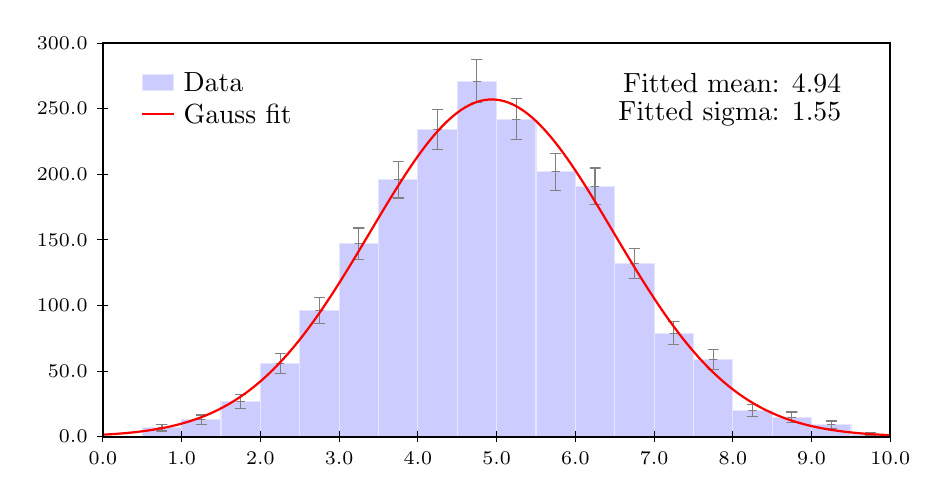
\begin{tikzpicture}
\node[left] at (9.5,4.5) {Fitted mean:  4.94};
\node[left] at (9.5,4.1) {Fitted sigma:  1.55};
\begin{scope}[]
\pgfpathmoveto{ \pgfpointxy {0.0} {0.0}}
\pgfpathlineto{ \pgfpointxy {10.0} {0.0}}
\pgfpathlineto{ \pgfpointxy {10.0} {5.0}}
\pgfpathlineto{ \pgfpointxy {0.0} {5.0}}
\pgfpathclose
\pgfusepath{  clip, }
\begin{scope}[shift={(0.0,0.0)}]
\pgfsetxvec{\pgfpoint{1.0cm}{0cm}}
\pgfsetyvec{\pgfpoint{0cm}{0.016666668cm}}
\begin{scope}[shift={(0.0,0.0)}]
\begin{scope}[draw=blue!10,fill=blue!20]
\pgfpathmoveto{ \pgfpointxy {10.0} {0.0}}
\pgfpathlineto{ \pgfpointxy {10.0} {2.0}}
\pgfpathlineto{ \pgfpointxy {9.5} {2.0}}
\pgfpathlineto{ \pgfpointxy {9.5} {9.0}}
\pgfpathlineto{ \pgfpointxy {9.0} {9.0}}
\pgfpathlineto{ \pgfpointxy {9.0} {15.0}}
\pgfpathlineto{ \pgfpointxy {8.5} {15.0}}
\pgfpathlineto{ \pgfpointxy {8.5} {20.0}}
\pgfpathlineto{ \pgfpointxy {8.0} {20.0}}
\pgfpathlineto{ \pgfpointxy {8.0} {59.0}}
\pgfpathlineto{ \pgfpointxy {7.5} {59.0}}
\pgfpathlineto{ \pgfpointxy {7.5} {79.0}}
\pgfpathlineto{ \pgfpointxy {7.0} {79.0}}
\pgfpathlineto{ \pgfpointxy {7.0} {132.0}}
\pgfpathlineto{ \pgfpointxy {6.5} {132.0}}
\pgfpathlineto{ \pgfpointxy {6.5} {191.0}}
\pgfpathlineto{ \pgfpointxy {6.0} {191.0}}
\pgfpathlineto{ \pgfpointxy {6.0} {202.0}}
\pgfpathlineto{ \pgfpointxy {5.5} {202.0}}
\pgfpathlineto{ \pgfpointxy {5.5} {242.0}}
\pgfpathlineto{ \pgfpointxy {5.0} {242.0}}
\pgfpathlineto{ \pgfpointxy {5.0} {271.0}}
\pgfpathlineto{ \pgfpointxy {4.5} {271.0}}
\pgfpathlineto{ \pgfpointxy {4.5} {234.0}}
\pgfpathlineto{ \pgfpointxy {4.0} {234.0}}
\pgfpathlineto{ \pgfpointxy {4.0} {196.0}}
\pgfpathlineto{ \pgfpointxy {3.5} {196.0}}
\pgfpathlineto{ \pgfpointxy {3.5} {147.0}}
\pgfpathlineto{ \pgfpointxy {3.0} {147.0}}
\pgfpathlineto{ \pgfpointxy {3.0} {96.0}}
\pgfpathlineto{ \pgfpointxy {2.5} {96.0}}
\pgfpathlineto{ \pgfpointxy {2.5} {56.0}}
\pgfpathlineto{ \pgfpointxy {2.0} {56.0}}
\pgfpathlineto{ \pgfpointxy {2.0} {27.0}}
\pgfpathlineto{ \pgfpointxy {1.5} {27.0}}
\pgfpathlineto{ \pgfpointxy {1.5} {13.0}}
\pgfpathlineto{ \pgfpointxy {1.0} {13.0}}
\pgfpathlineto{ \pgfpointxy {1.0} {7.0}}
\pgfpathlineto{ \pgfpointxy {0.5} {7.0}}
\pgfpathlineto{ \pgfpointxy {0.5} {0.0}}
\pgfpathlineto{ \pgfpointxy {0.0} {0.0}}
\pgfpathlineto{ \pgfpointxy {0.0} {0.0}}
\pgfusepath{ stroke, fill, }
\end{scope}
\begin{scope}[draw=blue!10,fill=blue!20]
\pgfpathmoveto{ \pgfpointxy {10.0} {0.0}}
\pgfpathlineto{ \pgfpointxy {10.0} {0.0}}
\pgfusepath{ stroke, }
\end{scope}
\begin{scope}[draw=blue!10,fill=blue!20]
\pgfpathmoveto{ \pgfpointxy {10.0} {2.0}}
\pgfpathlineto{ \pgfpointxy {10.0} {0.0}}
\pgfusepath{ stroke, }
\end{scope}
\begin{scope}[draw=blue!10,fill=blue!20]
\pgfpathmoveto{ \pgfpointxy {9.5} {2.0}}
\pgfpathlineto{ \pgfpointxy {9.5} {0.0}}
\pgfusepath{ stroke, }
\end{scope}
\begin{scope}[draw=blue!10,fill=blue!20]
\pgfpathmoveto{ \pgfpointxy {9.5} {9.0}}
\pgfpathlineto{ \pgfpointxy {9.5} {0.0}}
\pgfusepath{ stroke, }
\end{scope}
\begin{scope}[draw=blue!10,fill=blue!20]
\pgfpathmoveto{ \pgfpointxy {9.0} {9.0}}
\pgfpathlineto{ \pgfpointxy {9.0} {0.0}}
\pgfusepath{ stroke, }
\end{scope}
\begin{scope}[draw=blue!10,fill=blue!20]
\pgfpathmoveto{ \pgfpointxy {9.0} {15.0}}
\pgfpathlineto{ \pgfpointxy {9.0} {0.0}}
\pgfusepath{ stroke, }
\end{scope}
\begin{scope}[draw=blue!10,fill=blue!20]
\pgfpathmoveto{ \pgfpointxy {8.5} {15.0}}
\pgfpathlineto{ \pgfpointxy {8.5} {0.0}}
\pgfusepath{ stroke, }
\end{scope}
\begin{scope}[draw=blue!10,fill=blue!20]
\pgfpathmoveto{ \pgfpointxy {8.5} {20.0}}
\pgfpathlineto{ \pgfpointxy {8.5} {0.0}}
\pgfusepath{ stroke, }
\end{scope}
\begin{scope}[draw=blue!10,fill=blue!20]
\pgfpathmoveto{ \pgfpointxy {8.0} {20.0}}
\pgfpathlineto{ \pgfpointxy {8.0} {0.0}}
\pgfusepath{ stroke, }
\end{scope}
\begin{scope}[draw=blue!10,fill=blue!20]
\pgfpathmoveto{ \pgfpointxy {8.0} {59.0}}
\pgfpathlineto{ \pgfpointxy {8.0} {0.0}}
\pgfusepath{ stroke, }
\end{scope}
\begin{scope}[draw=blue!10,fill=blue!20]
\pgfpathmoveto{ \pgfpointxy {7.5} {59.0}}
\pgfpathlineto{ \pgfpointxy {7.5} {0.0}}
\pgfusepath{ stroke, }
\end{scope}
\begin{scope}[draw=blue!10,fill=blue!20]
\pgfpathmoveto{ \pgfpointxy {7.5} {79.0}}
\pgfpathlineto{ \pgfpointxy {7.5} {0.0}}
\pgfusepath{ stroke, }
\end{scope}
\begin{scope}[draw=blue!10,fill=blue!20]
\pgfpathmoveto{ \pgfpointxy {7.0} {79.0}}
\pgfpathlineto{ \pgfpointxy {7.0} {0.0}}
\pgfusepath{ stroke, }
\end{scope}
\begin{scope}[draw=blue!10,fill=blue!20]
\pgfpathmoveto{ \pgfpointxy {7.0} {132.0}}
\pgfpathlineto{ \pgfpointxy {7.0} {0.0}}
\pgfusepath{ stroke, }
\end{scope}
\begin{scope}[draw=blue!10,fill=blue!20]
\pgfpathmoveto{ \pgfpointxy {6.5} {132.0}}
\pgfpathlineto{ \pgfpointxy {6.5} {0.0}}
\pgfusepath{ stroke, }
\end{scope}
\begin{scope}[draw=blue!10,fill=blue!20]
\pgfpathmoveto{ \pgfpointxy {6.5} {191.0}}
\pgfpathlineto{ \pgfpointxy {6.5} {0.0}}
\pgfusepath{ stroke, }
\end{scope}
\begin{scope}[draw=blue!10,fill=blue!20]
\pgfpathmoveto{ \pgfpointxy {6.0} {191.0}}
\pgfpathlineto{ \pgfpointxy {6.0} {0.0}}
\pgfusepath{ stroke, }
\end{scope}
\begin{scope}[draw=blue!10,fill=blue!20]
\pgfpathmoveto{ \pgfpointxy {6.0} {202.0}}
\pgfpathlineto{ \pgfpointxy {6.0} {0.0}}
\pgfusepath{ stroke, }
\end{scope}
\begin{scope}[draw=blue!10,fill=blue!20]
\pgfpathmoveto{ \pgfpointxy {5.5} {202.0}}
\pgfpathlineto{ \pgfpointxy {5.5} {0.0}}
\pgfusepath{ stroke, }
\end{scope}
\begin{scope}[draw=blue!10,fill=blue!20]
\pgfpathmoveto{ \pgfpointxy {5.5} {242.0}}
\pgfpathlineto{ \pgfpointxy {5.5} {0.0}}
\pgfusepath{ stroke, }
\end{scope}
\begin{scope}[draw=blue!10,fill=blue!20]
\pgfpathmoveto{ \pgfpointxy {5.0} {242.0}}
\pgfpathlineto{ \pgfpointxy {5.0} {0.0}}
\pgfusepath{ stroke, }
\end{scope}
\begin{scope}[draw=blue!10,fill=blue!20]
\pgfpathmoveto{ \pgfpointxy {5.0} {271.0}}
\pgfpathlineto{ \pgfpointxy {5.0} {0.0}}
\pgfusepath{ stroke, }
\end{scope}
\begin{scope}[draw=blue!10,fill=blue!20]
\pgfpathmoveto{ \pgfpointxy {4.5} {271.0}}
\pgfpathlineto{ \pgfpointxy {4.5} {0.0}}
\pgfusepath{ stroke, }
\end{scope}
\begin{scope}[draw=blue!10,fill=blue!20]
\pgfpathmoveto{ \pgfpointxy {4.5} {234.0}}
\pgfpathlineto{ \pgfpointxy {4.5} {0.0}}
\pgfusepath{ stroke, }
\end{scope}
\begin{scope}[draw=blue!10,fill=blue!20]
\pgfpathmoveto{ \pgfpointxy {4.0} {234.0}}
\pgfpathlineto{ \pgfpointxy {4.0} {0.0}}
\pgfusepath{ stroke, }
\end{scope}
\begin{scope}[draw=blue!10,fill=blue!20]
\pgfpathmoveto{ \pgfpointxy {4.0} {196.0}}
\pgfpathlineto{ \pgfpointxy {4.0} {0.0}}
\pgfusepath{ stroke, }
\end{scope}
\begin{scope}[draw=blue!10,fill=blue!20]
\pgfpathmoveto{ \pgfpointxy {3.5} {196.0}}
\pgfpathlineto{ \pgfpointxy {3.5} {0.0}}
\pgfusepath{ stroke, }
\end{scope}
\begin{scope}[draw=blue!10,fill=blue!20]
\pgfpathmoveto{ \pgfpointxy {3.5} {147.0}}
\pgfpathlineto{ \pgfpointxy {3.5} {0.0}}
\pgfusepath{ stroke, }
\end{scope}
\begin{scope}[draw=blue!10,fill=blue!20]
\pgfpathmoveto{ \pgfpointxy {3.0} {147.0}}
\pgfpathlineto{ \pgfpointxy {3.0} {0.0}}
\pgfusepath{ stroke, }
\end{scope}
\begin{scope}[draw=blue!10,fill=blue!20]
\pgfpathmoveto{ \pgfpointxy {3.0} {96.0}}
\pgfpathlineto{ \pgfpointxy {3.0} {0.0}}
\pgfusepath{ stroke, }
\end{scope}
\begin{scope}[draw=blue!10,fill=blue!20]
\pgfpathmoveto{ \pgfpointxy {2.5} {96.0}}
\pgfpathlineto{ \pgfpointxy {2.5} {0.0}}
\pgfusepath{ stroke, }
\end{scope}
\begin{scope}[draw=blue!10,fill=blue!20]
\pgfpathmoveto{ \pgfpointxy {2.5} {56.0}}
\pgfpathlineto{ \pgfpointxy {2.5} {0.0}}
\pgfusepath{ stroke, }
\end{scope}
\begin{scope}[draw=blue!10,fill=blue!20]
\pgfpathmoveto{ \pgfpointxy {2.0} {56.0}}
\pgfpathlineto{ \pgfpointxy {2.0} {0.0}}
\pgfusepath{ stroke, }
\end{scope}
\begin{scope}[draw=blue!10,fill=blue!20]
\pgfpathmoveto{ \pgfpointxy {2.0} {27.0}}
\pgfpathlineto{ \pgfpointxy {2.0} {0.0}}
\pgfusepath{ stroke, }
\end{scope}
\begin{scope}[draw=blue!10,fill=blue!20]
\pgfpathmoveto{ \pgfpointxy {1.5} {27.0}}
\pgfpathlineto{ \pgfpointxy {1.5} {0.0}}
\pgfusepath{ stroke, }
\end{scope}
\begin{scope}[draw=blue!10,fill=blue!20]
\pgfpathmoveto{ \pgfpointxy {1.5} {13.0}}
\pgfpathlineto{ \pgfpointxy {1.5} {0.0}}
\pgfusepath{ stroke, }
\end{scope}
\begin{scope}[draw=blue!10,fill=blue!20]
\pgfpathmoveto{ \pgfpointxy {1.0} {13.0}}
\pgfpathlineto{ \pgfpointxy {1.0} {0.0}}
\pgfusepath{ stroke, }
\end{scope}
\begin{scope}[draw=blue!10,fill=blue!20]
\pgfpathmoveto{ \pgfpointxy {1.0} {7.0}}
\pgfpathlineto{ \pgfpointxy {1.0} {0.0}}
\pgfusepath{ stroke, }
\end{scope}
\begin{scope}[draw=blue!10,fill=blue!20]
\pgfpathmoveto{ \pgfpointxy {0.5} {7.0}}
\pgfpathlineto{ \pgfpointxy {0.5} {0.0}}
\pgfusepath{ stroke, }
\end{scope}
\begin{scope}[draw=blue!10,fill=blue!20]
\pgfpathmoveto{ \pgfpointxy {0.5} {0.0}}
\pgfpathlineto{ \pgfpointxy {0.5} {0.0}}
\pgfusepath{ stroke, }
\end{scope}
\begin{scope}[draw=blue!10,fill=blue!20]
\pgfpathmoveto{ \pgfpointxy {0.0} {0.0}}
\pgfpathlineto{ \pgfpointxy {0.0} {0.0}}
\pgfusepath{ stroke, }
\end{scope}
\begin{scope}[draw=blue!10,fill=blue!20]
\pgfpathmoveto{ \pgfpointxy {0.0} {0.0}}
\pgfpathlineto{ \pgfpointxy {0.0} {0.0}}
\pgfusepath{ stroke, }
\end{scope}
\begin{scope}[draw=gray,fill=gray]
\pgfpointadd{\pgfpointxy {0.25} {0.0}} {\pgfpoint{-2pt}{0}}\pgfpathmoveto{ NIL }
\pgfpointadd{\pgfpointxy {0.25} {0.0}} {\pgfpoint{2pt}{0}}\pgfpathlineto{ NIL }
\pgfpointadd{\pgfpointxy {0.25} {0.0}} {\pgfpoint{0pt}{0}}\pgfpathlineto{ NIL }
\pgfpointadd{\pgfpointxy {0.25} {0.0}} {\pgfpoint{0pt}{0}}\pgfpathlineto{ NIL }
\pgfpointadd{\pgfpointxy {0.25} {0.0}} {\pgfpoint{-2pt}{0}}\pgfpathlineto{ NIL }
\pgfpointadd{\pgfpointxy {0.25} {0.0}} {\pgfpoint{2pt}{0}}\pgfpathlineto{ NIL }
\pgfusepath{ stroke, }
\node at (0.25,0.0) [rectangle,inner sep=0.0pt,minimum width =3.0pt,minimum height=0.0pt,draw=gray,fill=gray] {}; 
\end{scope}
\begin{scope}[draw=gray,fill=gray]
\pgfpointadd{\pgfpointxy {0.75} {9.645751}} {\pgfpoint{-2pt}{0}}\pgfpathmoveto{ NIL }
\pgfpointadd{\pgfpointxy {0.75} {9.645751}} {\pgfpoint{2pt}{0}}\pgfpathlineto{ NIL }
\pgfpointadd{\pgfpointxy {0.75} {9.645751}} {\pgfpoint{0pt}{0}}\pgfpathlineto{ NIL }
\pgfpointadd{\pgfpointxy {0.75} {4.354249}} {\pgfpoint{0pt}{0}}\pgfpathlineto{ NIL }
\pgfpointadd{\pgfpointxy {0.75} {4.354249}} {\pgfpoint{-2pt}{0}}\pgfpathlineto{ NIL }
\pgfpointadd{\pgfpointxy {0.75} {4.354249}} {\pgfpoint{2pt}{0}}\pgfpathlineto{ NIL }
\pgfusepath{ stroke, }
\node at (0.75,7.0) [rectangle,inner sep=0.0pt,minimum width =3.0pt,minimum height=0.0pt,draw=gray,fill=gray] {}; 
\end{scope}
\begin{scope}[draw=gray,fill=gray]
\pgfpointadd{\pgfpointxy {1.25} {16.60555}} {\pgfpoint{-2pt}{0}}\pgfpathmoveto{ NIL }
\pgfpointadd{\pgfpointxy {1.25} {16.60555}} {\pgfpoint{2pt}{0}}\pgfpathlineto{ NIL }
\pgfpointadd{\pgfpointxy {1.25} {16.60555}} {\pgfpoint{0pt}{0}}\pgfpathlineto{ NIL }
\pgfpointadd{\pgfpointxy {1.25} {9.394449}} {\pgfpoint{0pt}{0}}\pgfpathlineto{ NIL }
\pgfpointadd{\pgfpointxy {1.25} {9.394449}} {\pgfpoint{-2pt}{0}}\pgfpathlineto{ NIL }
\pgfpointadd{\pgfpointxy {1.25} {9.394449}} {\pgfpoint{2pt}{0}}\pgfpathlineto{ NIL }
\pgfusepath{ stroke, }
\node at (1.25,13.0) [rectangle,inner sep=0.0pt,minimum width =3.0pt,minimum height=0.0pt,draw=gray,fill=gray] {}; 
\end{scope}
\begin{scope}[draw=gray,fill=gray]
\pgfpointadd{\pgfpointxy {1.75} {32.19615}} {\pgfpoint{-2pt}{0}}\pgfpathmoveto{ NIL }
\pgfpointadd{\pgfpointxy {1.75} {32.19615}} {\pgfpoint{2pt}{0}}\pgfpathlineto{ NIL }
\pgfpointadd{\pgfpointxy {1.75} {32.19615}} {\pgfpoint{0pt}{0}}\pgfpathlineto{ NIL }
\pgfpointadd{\pgfpointxy {1.75} {21.803848}} {\pgfpoint{0pt}{0}}\pgfpathlineto{ NIL }
\pgfpointadd{\pgfpointxy {1.75} {21.803848}} {\pgfpoint{-2pt}{0}}\pgfpathlineto{ NIL }
\pgfpointadd{\pgfpointxy {1.75} {21.803848}} {\pgfpoint{2pt}{0}}\pgfpathlineto{ NIL }
\pgfusepath{ stroke, }
\node at (1.75,27.0) [rectangle,inner sep=0.0pt,minimum width =3.0pt,minimum height=0.0pt,draw=gray,fill=gray] {}; 
\end{scope}
\begin{scope}[draw=gray,fill=gray]
\pgfpointadd{\pgfpointxy {2.25} {63.483315}} {\pgfpoint{-2pt}{0}}\pgfpathmoveto{ NIL }
\pgfpointadd{\pgfpointxy {2.25} {63.483315}} {\pgfpoint{2pt}{0}}\pgfpathlineto{ NIL }
\pgfpointadd{\pgfpointxy {2.25} {63.483315}} {\pgfpoint{0pt}{0}}\pgfpathlineto{ NIL }
\pgfpointadd{\pgfpointxy {2.25} {48.516685}} {\pgfpoint{0pt}{0}}\pgfpathlineto{ NIL }
\pgfpointadd{\pgfpointxy {2.25} {48.516685}} {\pgfpoint{-2pt}{0}}\pgfpathlineto{ NIL }
\pgfpointadd{\pgfpointxy {2.25} {48.516685}} {\pgfpoint{2pt}{0}}\pgfpathlineto{ NIL }
\pgfusepath{ stroke, }
\node at (2.25,56.0) [rectangle,inner sep=0.0pt,minimum width =3.0pt,minimum height=0.0pt,draw=gray,fill=gray] {}; 
\end{scope}
\begin{scope}[draw=gray,fill=gray]
\pgfpointadd{\pgfpointxy {2.75} {105.79796}} {\pgfpoint{-2pt}{0}}\pgfpathmoveto{ NIL }
\pgfpointadd{\pgfpointxy {2.75} {105.79796}} {\pgfpoint{2pt}{0}}\pgfpathlineto{ NIL }
\pgfpointadd{\pgfpointxy {2.75} {105.79796}} {\pgfpoint{0pt}{0}}\pgfpathlineto{ NIL }
\pgfpointadd{\pgfpointxy {2.75} {86.20204}} {\pgfpoint{0pt}{0}}\pgfpathlineto{ NIL }
\pgfpointadd{\pgfpointxy {2.75} {86.20204}} {\pgfpoint{-2pt}{0}}\pgfpathlineto{ NIL }
\pgfpointadd{\pgfpointxy {2.75} {86.20204}} {\pgfpoint{2pt}{0}}\pgfpathlineto{ NIL }
\pgfusepath{ stroke, }
\node at (2.75,96.0) [rectangle,inner sep=0.0pt,minimum width =3.0pt,minimum height=0.0pt,draw=gray,fill=gray] {}; 
\end{scope}
\begin{scope}[draw=gray,fill=gray]
\pgfpointadd{\pgfpointxy {3.25} {159.12436}} {\pgfpoint{-2pt}{0}}\pgfpathmoveto{ NIL }
\pgfpointadd{\pgfpointxy {3.25} {159.12436}} {\pgfpoint{2pt}{0}}\pgfpathlineto{ NIL }
\pgfpointadd{\pgfpointxy {3.25} {159.12436}} {\pgfpoint{0pt}{0}}\pgfpathlineto{ NIL }
\pgfpointadd{\pgfpointxy {3.25} {134.87564}} {\pgfpoint{0pt}{0}}\pgfpathlineto{ NIL }
\pgfpointadd{\pgfpointxy {3.25} {134.87564}} {\pgfpoint{-2pt}{0}}\pgfpathlineto{ NIL }
\pgfpointadd{\pgfpointxy {3.25} {134.87564}} {\pgfpoint{2pt}{0}}\pgfpathlineto{ NIL }
\pgfusepath{ stroke, }
\node at (3.25,147.0) [rectangle,inner sep=0.0pt,minimum width =3.0pt,minimum height=0.0pt,draw=gray,fill=gray] {}; 
\end{scope}
\begin{scope}[draw=gray,fill=gray]
\pgfpointadd{\pgfpointxy {3.75} {210.0}} {\pgfpoint{-2pt}{0}}\pgfpathmoveto{ NIL }
\pgfpointadd{\pgfpointxy {3.75} {210.0}} {\pgfpoint{2pt}{0}}\pgfpathlineto{ NIL }
\pgfpointadd{\pgfpointxy {3.75} {210.0}} {\pgfpoint{0pt}{0}}\pgfpathlineto{ NIL }
\pgfpointadd{\pgfpointxy {3.75} {182.0}} {\pgfpoint{0pt}{0}}\pgfpathlineto{ NIL }
\pgfpointadd{\pgfpointxy {3.75} {182.0}} {\pgfpoint{-2pt}{0}}\pgfpathlineto{ NIL }
\pgfpointadd{\pgfpointxy {3.75} {182.0}} {\pgfpoint{2pt}{0}}\pgfpathlineto{ NIL }
\pgfusepath{ stroke, }
\node at (3.75,196.0) [rectangle,inner sep=0.0pt,minimum width =3.0pt,minimum height=0.0pt,draw=gray,fill=gray] {}; 
\end{scope}
\begin{scope}[draw=gray,fill=gray]
\pgfpointadd{\pgfpointxy {4.25} {249.29706}} {\pgfpoint{-2pt}{0}}\pgfpathmoveto{ NIL }
\pgfpointadd{\pgfpointxy {4.25} {249.29706}} {\pgfpoint{2pt}{0}}\pgfpathlineto{ NIL }
\pgfpointadd{\pgfpointxy {4.25} {249.29706}} {\pgfpoint{0pt}{0}}\pgfpathlineto{ NIL }
\pgfpointadd{\pgfpointxy {4.25} {218.70294}} {\pgfpoint{0pt}{0}}\pgfpathlineto{ NIL }
\pgfpointadd{\pgfpointxy {4.25} {218.70294}} {\pgfpoint{-2pt}{0}}\pgfpathlineto{ NIL }
\pgfpointadd{\pgfpointxy {4.25} {218.70294}} {\pgfpoint{2pt}{0}}\pgfpathlineto{ NIL }
\pgfusepath{ stroke, }
\node at (4.25,234.0) [rectangle,inner sep=0.0pt,minimum width =3.0pt,minimum height=0.0pt,draw=gray,fill=gray] {}; 
\end{scope}
\begin{scope}[draw=gray,fill=gray]
\pgfpointadd{\pgfpointxy {4.75} {287.46207}} {\pgfpoint{-2pt}{0}}\pgfpathmoveto{ NIL }
\pgfpointadd{\pgfpointxy {4.75} {287.46207}} {\pgfpoint{2pt}{0}}\pgfpathlineto{ NIL }
\pgfpointadd{\pgfpointxy {4.75} {287.46207}} {\pgfpoint{0pt}{0}}\pgfpathlineto{ NIL }
\pgfpointadd{\pgfpointxy {4.75} {254.53792}} {\pgfpoint{0pt}{0}}\pgfpathlineto{ NIL }
\pgfpointadd{\pgfpointxy {4.75} {254.53792}} {\pgfpoint{-2pt}{0}}\pgfpathlineto{ NIL }
\pgfpointadd{\pgfpointxy {4.75} {254.53792}} {\pgfpoint{2pt}{0}}\pgfpathlineto{ NIL }
\pgfusepath{ stroke, }
\node at (4.75,271.0) [rectangle,inner sep=0.0pt,minimum width =3.0pt,minimum height=0.0pt,draw=gray,fill=gray] {}; 
\end{scope}
\begin{scope}[draw=gray,fill=gray]
\pgfpointadd{\pgfpointxy {5.25} {257.55634}} {\pgfpoint{-2pt}{0}}\pgfpathmoveto{ NIL }
\pgfpointadd{\pgfpointxy {5.25} {257.55634}} {\pgfpoint{2pt}{0}}\pgfpathlineto{ NIL }
\pgfpointadd{\pgfpointxy {5.25} {257.55634}} {\pgfpoint{0pt}{0}}\pgfpathlineto{ NIL }
\pgfpointadd{\pgfpointxy {5.25} {226.44365}} {\pgfpoint{0pt}{0}}\pgfpathlineto{ NIL }
\pgfpointadd{\pgfpointxy {5.25} {226.44365}} {\pgfpoint{-2pt}{0}}\pgfpathlineto{ NIL }
\pgfpointadd{\pgfpointxy {5.25} {226.44365}} {\pgfpoint{2pt}{0}}\pgfpathlineto{ NIL }
\pgfusepath{ stroke, }
\node at (5.25,242.0) [rectangle,inner sep=0.0pt,minimum width =3.0pt,minimum height=0.0pt,draw=gray,fill=gray] {}; 
\end{scope}
\begin{scope}[draw=gray,fill=gray]
\pgfpointadd{\pgfpointxy {5.75} {216.21268}} {\pgfpoint{-2pt}{0}}\pgfpathmoveto{ NIL }
\pgfpointadd{\pgfpointxy {5.75} {216.21268}} {\pgfpoint{2pt}{0}}\pgfpathlineto{ NIL }
\pgfpointadd{\pgfpointxy {5.75} {216.21268}} {\pgfpoint{0pt}{0}}\pgfpathlineto{ NIL }
\pgfpointadd{\pgfpointxy {5.75} {187.78732}} {\pgfpoint{0pt}{0}}\pgfpathlineto{ NIL }
\pgfpointadd{\pgfpointxy {5.75} {187.78732}} {\pgfpoint{-2pt}{0}}\pgfpathlineto{ NIL }
\pgfpointadd{\pgfpointxy {5.75} {187.78732}} {\pgfpoint{2pt}{0}}\pgfpathlineto{ NIL }
\pgfusepath{ stroke, }
\node at (5.75,202.0) [rectangle,inner sep=0.0pt,minimum width =3.0pt,minimum height=0.0pt,draw=gray,fill=gray] {}; 
\end{scope}
\begin{scope}[draw=gray,fill=gray]
\pgfpointadd{\pgfpointxy {6.25} {204.82028}} {\pgfpoint{-2pt}{0}}\pgfpathmoveto{ NIL }
\pgfpointadd{\pgfpointxy {6.25} {204.82028}} {\pgfpoint{2pt}{0}}\pgfpathlineto{ NIL }
\pgfpointadd{\pgfpointxy {6.25} {204.82028}} {\pgfpoint{0pt}{0}}\pgfpathlineto{ NIL }
\pgfpointadd{\pgfpointxy {6.25} {177.17972}} {\pgfpoint{0pt}{0}}\pgfpathlineto{ NIL }
\pgfpointadd{\pgfpointxy {6.25} {177.17972}} {\pgfpoint{-2pt}{0}}\pgfpathlineto{ NIL }
\pgfpointadd{\pgfpointxy {6.25} {177.17972}} {\pgfpoint{2pt}{0}}\pgfpathlineto{ NIL }
\pgfusepath{ stroke, }
\node at (6.25,191.0) [rectangle,inner sep=0.0pt,minimum width =3.0pt,minimum height=0.0pt,draw=gray,fill=gray] {}; 
\end{scope}
\begin{scope}[draw=gray,fill=gray]
\pgfpointadd{\pgfpointxy {6.75} {143.48912}} {\pgfpoint{-2pt}{0}}\pgfpathmoveto{ NIL }
\pgfpointadd{\pgfpointxy {6.75} {143.48912}} {\pgfpoint{2pt}{0}}\pgfpathlineto{ NIL }
\pgfpointadd{\pgfpointxy {6.75} {143.48912}} {\pgfpoint{0pt}{0}}\pgfpathlineto{ NIL }
\pgfpointadd{\pgfpointxy {6.75} {120.51087}} {\pgfpoint{0pt}{0}}\pgfpathlineto{ NIL }
\pgfpointadd{\pgfpointxy {6.75} {120.51087}} {\pgfpoint{-2pt}{0}}\pgfpathlineto{ NIL }
\pgfpointadd{\pgfpointxy {6.75} {120.51087}} {\pgfpoint{2pt}{0}}\pgfpathlineto{ NIL }
\pgfusepath{ stroke, }
\node at (6.75,132.0) [rectangle,inner sep=0.0pt,minimum width =3.0pt,minimum height=0.0pt,draw=gray,fill=gray] {}; 
\end{scope}
\begin{scope}[draw=gray,fill=gray]
\pgfpointadd{\pgfpointxy {7.25} {87.88819}} {\pgfpoint{-2pt}{0}}\pgfpathmoveto{ NIL }
\pgfpointadd{\pgfpointxy {7.25} {87.88819}} {\pgfpoint{2pt}{0}}\pgfpathlineto{ NIL }
\pgfpointadd{\pgfpointxy {7.25} {87.88819}} {\pgfpoint{0pt}{0}}\pgfpathlineto{ NIL }
\pgfpointadd{\pgfpointxy {7.25} {70.11181}} {\pgfpoint{0pt}{0}}\pgfpathlineto{ NIL }
\pgfpointadd{\pgfpointxy {7.25} {70.11181}} {\pgfpoint{-2pt}{0}}\pgfpathlineto{ NIL }
\pgfpointadd{\pgfpointxy {7.25} {70.11181}} {\pgfpoint{2pt}{0}}\pgfpathlineto{ NIL }
\pgfusepath{ stroke, }
\node at (7.25,79.0) [rectangle,inner sep=0.0pt,minimum width =3.0pt,minimum height=0.0pt,draw=gray,fill=gray] {}; 
\end{scope}
\begin{scope}[draw=gray,fill=gray]
\pgfpointadd{\pgfpointxy {7.75} {66.681145}} {\pgfpoint{-2pt}{0}}\pgfpathmoveto{ NIL }
\pgfpointadd{\pgfpointxy {7.75} {66.681145}} {\pgfpoint{2pt}{0}}\pgfpathlineto{ NIL }
\pgfpointadd{\pgfpointxy {7.75} {66.681145}} {\pgfpoint{0pt}{0}}\pgfpathlineto{ NIL }
\pgfpointadd{\pgfpointxy {7.75} {51.318855}} {\pgfpoint{0pt}{0}}\pgfpathlineto{ NIL }
\pgfpointadd{\pgfpointxy {7.75} {51.318855}} {\pgfpoint{-2pt}{0}}\pgfpathlineto{ NIL }
\pgfpointadd{\pgfpointxy {7.75} {51.318855}} {\pgfpoint{2pt}{0}}\pgfpathlineto{ NIL }
\pgfusepath{ stroke, }
\node at (7.75,59.0) [rectangle,inner sep=0.0pt,minimum width =3.0pt,minimum height=0.0pt,draw=gray,fill=gray] {}; 
\end{scope}
\begin{scope}[draw=gray,fill=gray]
\pgfpointadd{\pgfpointxy {8.25} {24.472136}} {\pgfpoint{-2pt}{0}}\pgfpathmoveto{ NIL }
\pgfpointadd{\pgfpointxy {8.25} {24.472136}} {\pgfpoint{2pt}{0}}\pgfpathlineto{ NIL }
\pgfpointadd{\pgfpointxy {8.25} {24.472136}} {\pgfpoint{0pt}{0}}\pgfpathlineto{ NIL }
\pgfpointadd{\pgfpointxy {8.25} {15.527864}} {\pgfpoint{0pt}{0}}\pgfpathlineto{ NIL }
\pgfpointadd{\pgfpointxy {8.25} {15.527864}} {\pgfpoint{-2pt}{0}}\pgfpathlineto{ NIL }
\pgfpointadd{\pgfpointxy {8.25} {15.527864}} {\pgfpoint{2pt}{0}}\pgfpathlineto{ NIL }
\pgfusepath{ stroke, }
\node at (8.25,20.0) [rectangle,inner sep=0.0pt,minimum width =3.0pt,minimum height=0.0pt,draw=gray,fill=gray] {}; 
\end{scope}
\begin{scope}[draw=gray,fill=gray]
\pgfpointadd{\pgfpointxy {8.75} {18.872984}} {\pgfpoint{-2pt}{0}}\pgfpathmoveto{ NIL }
\pgfpointadd{\pgfpointxy {8.75} {18.872984}} {\pgfpoint{2pt}{0}}\pgfpathlineto{ NIL }
\pgfpointadd{\pgfpointxy {8.75} {18.872984}} {\pgfpoint{0pt}{0}}\pgfpathlineto{ NIL }
\pgfpointadd{\pgfpointxy {8.75} {11.127016}} {\pgfpoint{0pt}{0}}\pgfpathlineto{ NIL }
\pgfpointadd{\pgfpointxy {8.75} {11.127016}} {\pgfpoint{-2pt}{0}}\pgfpathlineto{ NIL }
\pgfpointadd{\pgfpointxy {8.75} {11.127016}} {\pgfpoint{2pt}{0}}\pgfpathlineto{ NIL }
\pgfusepath{ stroke, }
\node at (8.75,15.0) [rectangle,inner sep=0.0pt,minimum width =3.0pt,minimum height=0.0pt,draw=gray,fill=gray] {}; 
\end{scope}
\begin{scope}[draw=gray,fill=gray]
\pgfpointadd{\pgfpointxy {9.25} {12.0}} {\pgfpoint{-2pt}{0}}\pgfpathmoveto{ NIL }
\pgfpointadd{\pgfpointxy {9.25} {12.0}} {\pgfpoint{2pt}{0}}\pgfpathlineto{ NIL }
\pgfpointadd{\pgfpointxy {9.25} {12.0}} {\pgfpoint{0pt}{0}}\pgfpathlineto{ NIL }
\pgfpointadd{\pgfpointxy {9.25} {6.0}} {\pgfpoint{0pt}{0}}\pgfpathlineto{ NIL }
\pgfpointadd{\pgfpointxy {9.25} {6.0}} {\pgfpoint{-2pt}{0}}\pgfpathlineto{ NIL }
\pgfpointadd{\pgfpointxy {9.25} {6.0}} {\pgfpoint{2pt}{0}}\pgfpathlineto{ NIL }
\pgfusepath{ stroke, }
\node at (9.25,9.0) [rectangle,inner sep=0.0pt,minimum width =3.0pt,minimum height=0.0pt,draw=gray,fill=gray] {}; 
\end{scope}
\begin{scope}[draw=gray,fill=gray]
\pgfpointadd{\pgfpointxy {9.75} {3.4142137}} {\pgfpoint{-2pt}{0}}\pgfpathmoveto{ NIL }
\pgfpointadd{\pgfpointxy {9.75} {3.4142137}} {\pgfpoint{2pt}{0}}\pgfpathlineto{ NIL }
\pgfpointadd{\pgfpointxy {9.75} {3.4142137}} {\pgfpoint{0pt}{0}}\pgfpathlineto{ NIL }
\pgfpointadd{\pgfpointxy {9.75} {0.58578646}} {\pgfpoint{0pt}{0}}\pgfpathlineto{ NIL }
\pgfpointadd{\pgfpointxy {9.75} {0.58578646}} {\pgfpoint{-2pt}{0}}\pgfpathlineto{ NIL }
\pgfpointadd{\pgfpointxy {9.75} {0.58578646}} {\pgfpoint{2pt}{0}}\pgfpathlineto{ NIL }
\pgfusepath{ stroke, }
\node at (9.75,2.0) [rectangle,inner sep=0.0pt,minimum width =3.0pt,minimum height=0.0pt,draw=gray,fill=gray] {}; 
\end{scope}
\begin{scope}[thick,red]
\pgfpathmoveto{ \pgfpointxy {0.0} {1.558576020676866}}
\pgfpathlineto{ \pgfpointxy {0.05} {1.7274503227501066}}
\pgfpathlineto{ \pgfpointxy {0.1} {1.9126188963667363}}
\pgfpathlineto{ \pgfpointxy {0.15} {2.1154200480403227}}
\pgfpathlineto{ \pgfpointxy {0.2} {2.3372764756403903}}
\pgfpathlineto{ \pgfpointxy {0.25} {2.5796979496539985}}
\pgfpathlineto{ \pgfpointxy {0.3} {2.8442837980858506}}
\pgfpathlineto{ \pgfpointxy {0.35} {3.132725158018863}}
\pgfpathlineto{ \pgfpointxy {0.4} {3.4468069547981615}}
\pgfpathlineto{ \pgfpointxy {0.45} {3.7884095678724714}}
\pgfpathlineto{ \pgfpointxy {0.5} {4.159510140559981}}
\pgfpathlineto{ \pgfpointxy {0.55} {4.562183489434911}}
\pgfpathlineto{ \pgfpointxy {0.6} {4.99860256769178}}
\pgfpathlineto{ \pgfpointxy {0.65} {5.471038435772837}}
\pgfpathlineto{ \pgfpointxy {0.7} {5.981859691776892}}
\pgfpathlineto{ \pgfpointxy {0.75} {6.533531313743065}}
\pgfpathlineto{ \pgfpointxy {0.8} {7.128612865856165}}
\pgfpathlineto{ \pgfpointxy {0.85} {7.769756020989981}}
\pgfpathlineto{ \pgfpointxy {0.9} {8.459701352824242}}
\pgfpathlineto{ \pgfpointxy {0.95} {9.201274352075282}}
\pgfpathlineto{ \pgfpointxy {1.0} {9.997380623200701}}
\pgfpathlineto{ \pgfpointxy {1.05} {10.85100022030292}}
\pgfpathlineto{ \pgfpointxy {1.1} {11.765181083891807}}
\pgfpathlineto{ \pgfpointxy {1.15} {12.74303154369313}}
\pgfpathlineto{ \pgfpointxy {1.2} {13.78771185682457}}
\pgfpathlineto{ \pgfpointxy {1.25} {14.902424755416321}}
\pgfpathlineto{ \pgfpointxy {1.3} {16.090404983135112}}
\pgfpathlineto{ \pgfpointxy {1.35} {17.354907806077094}}
\pgfpathlineto{ \pgfpointxy {1.4} {18.699196490121263}}
\pgfpathlineto{ \pgfpointxy {1.45} {20.12652874406518}}
\pgfpathlineto{ \pgfpointxy {1.5} {21.640142135675536}}
\pgfpathlineto{ \pgfpointxy {1.55} {23.24323849615082}}
\pgfpathlineto{ \pgfpointxy {1.6} {24.938967337367576}}
\pgfpathlineto{ \pgfpointxy {1.65} {26.7304083156247}}
\pgfpathlineto{ \pgfpointxy {1.7} {28.62055278535065}}
\pgfpathlineto{ \pgfpointxy {1.75} {30.612284496334055}}
\pgfpathlineto{ \pgfpointxy {1.8} {32.70835949840771}}
\pgfpathlineto{ \pgfpointxy {1.85} {34.91138532807266}}
\pgfpathlineto{ \pgfpointxy {1.9} {37.22379956221061}}
\pgfpathlineto{ \pgfpointxy {1.95} {39.64784783469681}}
\pgfpathlineto{ \pgfpointxy {2.0} {42.185561422291414}}
\pgfpathlineto{ \pgfpointxy {2.05} {44.838734516545586}}
\pgfpathlineto{ \pgfpointxy {2.1} {47.60890130849298}}
\pgfpathlineto{ \pgfpointxy {2.15} {50.4973130224912}}
\pgfpathlineto{ \pgfpointxy {2.2} {53.504915044608836}}
\pgfpathlineto{ \pgfpointxy {2.25} {56.632324299297366}}
\pgfpathlineto{ \pgfpointxy {2.3} {59.87980703562242}}
\pgfpathlineto{ \pgfpointxy {2.35} {63.24725719093013}}
\pgfpathlineto{ \pgfpointxy {2.4} {66.73417550537421}}
\pgfpathlineto{ \pgfpointxy {2.45} {70.33964956511109}}
\pgfpathlineto{ \pgfpointxy {2.5} {74.06233495507152}}
\pgfpathlineto{ \pgfpointxy {2.55} {77.90043770394169}}
\pgfpathlineto{ \pgfpointxy {2.6} {81.85169820423305}}
\pgfpathlineto{ \pgfpointxy {2.65} {85.91337678901114}}
\pgfpathlineto{ \pgfpointxy {2.7} {90.08224114391795}}
\pgfpathlineto{ \pgfpointxy {2.75} {94.35455572849908}}
\pgfpathlineto{ \pgfpointxy {2.8} {98.72607337450253}}
\pgfpathlineto{ \pgfpointxy {2.85} {103.19202922071392}}
\pgfpathlineto{ \pgfpointxy {2.9} {107.74713713403635}}
\pgfpathlineto{ \pgfpointxy {2.95} {112.38558875491714}}
\pgfpathlineto{ \pgfpointxy {3.0} {117.10105529189481}}
\pgfpathlineto{ \pgfpointxy {3.05} {121.88669217504761}}
\pgfpathlineto{ \pgfpointxy {3.1} {126.73514666152779}}
\pgfpathlineto{ \pgfpointxy {3.15} {131.63856846826192}}
\pgfpathlineto{ \pgfpointxy {3.2} {136.58862348739274}}
\pgfpathlineto{ \pgfpointxy {3.25} {141.57651061926111}}
\pgfpathlineto{ \pgfpointxy {3.3} {146.59298173583076}}
\pgfpathlineto{ \pgfpointxy {3.35} {151.62836476460035}}
\pgfpathlineto{ \pgfpointxy {3.4} {156.67258985942038}}
\pgfpathlineto{ \pgfpointxy {3.45} {161.7152186004281}}
\pgfpathlineto{ \pgfpointxy {3.5} {166.74547614073975}}
\pgfpathlineto{ \pgfpointxy {3.55} {171.75228619282998}}
\pgfpathlineto{ \pgfpointxy {3.6} {176.72430872290073}}
\pgfpathlineto{ \pgfpointxy {3.65} {181.6499801972455}}
\pgfpathlineto{ \pgfpointxy {3.7} {186.5175562008881}}
\pgfpathlineto{ \pgfpointxy {3.75} {191.31515622585772}}
\pgfpathlineto{ \pgfpointxy {3.8} {196.03081040460765}}
\pgfpathlineto{ \pgfpointxy {3.85} {200.65250794351792}}
\pgfpathlineto{ \pgfpointxy {3.9} {205.1682469923884}}
\pgfpathlineto{ \pgfpointxy {3.95} {209.56608566853743}}
\pgfpathlineto{ \pgfpointxy {4.0} {213.83419393878864}}
\pgfpathlineto{ \pgfpointxy {4.05} {217.9609060494452}}
\pgfpathlineto{ \pgfpointxy {4.1} {221.93477318349133}}
\pgfpathlineto{ \pgfpointxy {4.15} {225.74461601588078}}
\pgfpathlineto{ \pgfpointxy {4.2} {229.3795768320013}}
\pgfpathlineto{ \pgfpointxy {4.25} {232.82917087135112}}
\pgfpathlineto{ \pgfpointxy {4.3} {236.08333655820527}}
\pgfpathlineto{ \pgfpointxy {4.35} {239.13248428364233}}
\pgfpathlineto{ \pgfpointxy {4.4} {241.9675434087641}}
\pgfpathlineto{ \pgfpointxy {4.45} {244.58000716726772}}
\pgfpathlineto{ \pgfpointxy {4.5} {246.9619751566839}}
\pgfpathlineto{ \pgfpointxy {4.55} {249.1061931215066}}
\pgfpathlineto{ \pgfpointxy {4.6} {251.00608974801486}}
\pgfpathlineto{ \pgfpointxy {4.65} {252.6558102096966}}
\pgfpathlineto{ \pgfpointxy {4.7} {254.05024622367264}}
\pgfpathlineto{ \pgfpointxy {4.75} {255.18506240220933}}
\pgfpathlineto{ \pgfpointxy {4.8} {256.0567187090879}}
\pgfpathlineto{ \pgfpointxy {4.85} {256.6624888580471}}
\pgfpathlineto{ \pgfpointxy {4.9} {257.0004745194776}}
\pgfpathlineto{ \pgfpointxy {4.95} {257.06961523176074}}
\pgfpathlineto{ \pgfpointxy {5.0} {256.86969394483054}}
\pgfpathlineto{ \pgfpointxy {5.05} {256.401338155402}}
\pgfpathlineto{ \pgfpointxy {5.1} {255.66601662555647}}
\pgfpathlineto{ \pgfpointxy {5.15} {254.66603170869865}}
\pgfpathlineto{ \pgfpointxy {5.2} {253.40450733900056}}
\pgfpathlineto{ \pgfpointxy {5.25} {251.88537277201746}}
\pgfpathlineto{ \pgfpointxy {5.3} {250.11334219491098}}
\pgfpathlineto{ \pgfpointxy {5.35} {248.0938903543545}}
\pgfpathlineto{ \pgfpointxy {5.4} {245.83322437845325}}
\pgfpathlineto{ \pgfpointxy {5.45} {243.33825199563105}}
\pgfpathlineto{ \pgfpointxy {5.5} {240.61654637817384}}
\pgfpathlineto{ \pgfpointxy {5.55} {237.6763078607661}}
\pgfpathlineto{ \pgfpointxy {5.6} {234.52632280470687}}
\pgfpathlineto{ \pgfpointxy {5.65} {231.17591989638905}}
\pgfpathlineto{ \pgfpointxy {5.7} {227.63492418391843}}
\pgfpathlineto{ \pgfpointxy {5.75} {223.9136091683304}}
\pgfpathlineto{ \pgfpointxy {5.8} {220.02264727565102}}
\pgfpathlineto{ \pgfpointxy {5.85} {215.9730590429822}}
\pgfpathlineto{ \pgfpointxy {5.9} {211.77616135586024}}
\pgfpathlineto{ \pgfpointxy {5.95} {207.44351507533685}}
\pgfpathlineto{ \pgfpointxy {6.0} {202.9868723916073}}
\pgfpathlineto{ \pgfpointxy {6.05} {198.41812423662532}}
\pgfpathlineto{ \pgfpointxy {6.1} {193.74924808108875}}
\pgfpathlineto{ \pgfpointxy {6.15} {188.99225643157735}}
\pgfpathlineto{ \pgfpointxy {6.2} {184.1591463316151}}
\pgfpathlineto{ \pgfpointxy {6.25} {179.26185015617526}}
\pgfpathlineto{ \pgfpointxy {6.3} {174.31218797284095}}
\pgfpathlineto{ \pgfpointxy {6.35} {169.32182172466466}}
\pgfpathlineto{ \pgfpointxy {6.4} {164.30221146996436}}
\pgfpathlineto{ \pgfpointxy {6.45} {159.26457389307188}}
\pgfpathlineto{ \pgfpointxy {6.5} {154.21984327764548}}
\pgfpathlineto{ \pgfpointxy {6.55} {149.17863511082155}}
\pgfpathlineto{ \pgfpointxy {6.6} {144.151212462442}}
\pgfpathlineto{ \pgfpointxy {6.65} {139.14745525910845}}
\pgfpathlineto{ \pgfpointxy {6.7} {134.17683254811797}}
\pgfpathlineto{ \pgfpointxy {6.75} {129.24837782166048}}
\pgfpathlineto{ \pgfpointxy {6.8} {124.37066744724133}}
\pgfpathlineto{ \pgfpointxy {6.85} {119.55180222633848}}
\pgfpathlineto{ \pgfpointxy {6.9} {114.79939208002902}}
\pgfpathlineto{ \pgfpointxy {6.95} {110.12054383790831}}
\pgfpathlineto{ \pgfpointxy {7.0} {105.52185208525077}}
\pgfpathlineto{ \pgfpointxy {7.05} {101.00939300318913}}
\pgfpathlineto{ \pgfpointxy {7.1} {96.58872111784704}}
\pgfpathlineto{ \pgfpointxy {7.15} {92.26486885697777}}
\pgfpathlineto{ \pgfpointxy {7.2} {88.04234879683506}}
\pgfpathlineto{ \pgfpointxy {7.25} {83.92515846780941}}
\pgfpathlineto{ \pgfpointxy {7.3} {79.91678757487001}}
\pgfpathlineto{ \pgfpointxy {7.35} {76.02022747809175}}
\pgfpathlineto{ \pgfpointxy {7.4} {72.23798276954341}}
\pgfpathlineto{ \pgfpointxy {7.45} {68.57208477556978}}
\pgfpathlineto{ \pgfpointxy {7.5} {65.02410680799369}}
\pgfpathlineto{ \pgfpointxy {7.55} {61.59518098397015}}
\pgfpathlineto{ \pgfpointxy {7.6} {58.28601643208637}}
\pgfpathlineto{ \pgfpointxy {7.65} {55.09691870175808}}
\pgfpathlineto{ \pgfpointxy {7.7} {52.02781019395011}}
\pgfpathlineto{ \pgfpointxy {7.75} {49.07825143365233}}
\pgfpathlineto{ \pgfpointxy {7.8} {46.24746300828272}}
\pgfpathlineto{ \pgfpointxy {7.85} {43.53434800114982}}
\pgfpathlineto{ \pgfpointxy {7.9} {40.937514755184765}}
\pgfpathlineto{ \pgfpointxy {7.95} {38.45529980922224}}
\pgfpathlineto{ \pgfpointxy {8.0} {36.085790857054135}}
\pgfpathlineto{ \pgfpointxy {8.05} {33.82684958817274}}
\pgfpathlineto{ \pgfpointxy {8.1} {31.6761342784406}}
\pgfpathlineto{ \pgfpointxy {8.15} {29.631122008746036}}
\pgfpathlineto{ \pgfpointxy {8.2} {27.689130399912187}}
\pgfpathlineto{ \pgfpointxy {8.25} {25.847338762597456}}
\pgfpathlineto{ \pgfpointxy {8.3} {24.10280857155552}}
\pgfpathlineto{ \pgfpointxy {8.35} {22.452503184295036}}
\pgfpathlineto{ \pgfpointxy {8.4} {20.89330673480372}}
\pgfpathlineto{ \pgfpointxy {8.45} {19.42204214347753}}
\pgfpathlineto{ \pgfpointxy {8.5} {18.03548819463977}}
\pgfpathlineto{ \pgfpointxy {8.55} {16.73039564297438}}
\pgfpathlineto{ \pgfpointxy {8.6} {15.503502319754952}}
\pgfpathlineto{ \pgfpointxy {8.65} {14.351547218873485}}
\pgfpathlineto{ \pgfpointxy {8.7} {13.271283551305883}}
\pgfpathlineto{ \pgfpointxy {8.75} {12.259490764748348}}
\pgfpathlineto{ \pgfpointxy {8.8} {11.312985532693581}}
\pgfpathlineto{ \pgfpointxy {8.85} {10.428631724151984}}
\pgfpathlineto{ \pgfpointxy {8.9} {9.603349371550834}}
\pgfpathlineto{ \pgfpointxy {8.95} {8.834122660047734}}
\pgfpathlineto{ \pgfpointxy {9.0} {8.118006966570197}}
\pgfpathlineto{ \pgfpointxy {9.05} {7.452134981347872}}
\pgfpathlineto{ \pgfpointxy {9.1} {6.8337219485391705}}
\pgfpathlineto{ \pgfpointxy {9.15} {6.260070065792449}}
\pgfpathlineto{ \pgfpointxy {9.2} {5.72857208523604}}
\pgfpathlineto{ \pgfpointxy {9.25} {5.236714160487787}}
\pgfpathlineto{ \pgfpointxy {9.3} {4.78207798584115}}
\pgfpathlineto{ \pgfpointxy {9.35} {4.362342274848571}}
\pgfpathlineto{ \pgfpointxy {9.4} {3.975283626119874}}
\pgfpathlineto{ \pgfpointxy {9.45} {3.6187768243158493}}
\pgfpathlineto{ \pgfpointxy {9.5} {3.290794624081893}}
\pgfpathlineto{ \pgfpointxy {9.55} {2.9894070640710915}}
\pgfpathlineto{ \pgfpointxy {9.6} {2.712780357285991}}
\pgfpathlineto{ \pgfpointxy {9.65} {2.459175402762056}}
\pgfpathlineto{ \pgfpointxy {9.7} {2.2269459621598866}}
\pgfpathlineto{ \pgfpointxy {9.75} {2.014536543162128}}
\pgfpathlineto{ \pgfpointxy {9.8} {1.8204800297218426}}
\pgfpathlineto{ \pgfpointxy {9.85} {1.6433950972124476}}
\pgfpathlineto{ \pgfpointxy {9.9} {1.4819834484189018}}
\pgfpathlineto{ \pgfpointxy {9.95} {1.335026904114285}}
\pgfpathlineto{ \pgfpointxy {10.0} {1.2013843797131074}}
\pgfusepath{ stroke, }
\end{scope}
\end{scope}
\pgfsetxvec{\pgfpoint{1cm}{0cm}}
\pgfsetyvec{\pgfpoint{0cm}{1cm}}
\end{scope}
\end{scope}
\begin{scope}[shift={(0.0,0.0)}]
\pgfsetxvec{\pgfpoint{1.0cm}{0cm}}
\pgfsetyvec{\pgfpoint{0cm}{0.016666668cm}}
\begin{scope}[shift={(0.0,0.0)}]
\begin{scope}[thick,black,fill=white]
\pgfpathmoveto{ \pgfpointxy {0.0} {0.0}}
\pgfpathlineto{ \pgfpointxy {10.0} {0.0}}
\pgfpathlineto{ \pgfpointxy {10.0} {300.0}}
\pgfpathlineto{ \pgfpointxy {0.0} {300.0}}
\pgfpathclose
\pgfusepath{ stroke, }
\end{scope}
\begin{scope}[yshift=0cm]
\draw[] [shift={(0.0,0.0)}] (0,2pt) -- (0,-2pt) node[below]{ \scriptsize{\num[round-mode=places,round-precision=1]{0.0}}};
\draw[] [shift={(1.0,0.0)}] (0,2pt) -- (0,-2pt) node[below]{ \scriptsize{\num[round-mode=places,round-precision=1]{1.0}}};
\draw[] [shift={(2.0,0.0)}] (0,2pt) -- (0,-2pt) node[below]{ \scriptsize{\num[round-mode=places,round-precision=1]{2.0}}};
\draw[] [shift={(3.0,0.0)}] (0,2pt) -- (0,-2pt) node[below]{ \scriptsize{\num[round-mode=places,round-precision=1]{3.0}}};
\draw[] [shift={(4.0,0.0)}] (0,2pt) -- (0,-2pt) node[below]{ \scriptsize{\num[round-mode=places,round-precision=1]{4.0}}};
\draw[] [shift={(5.0,0.0)}] (0,2pt) -- (0,-2pt) node[below]{ \scriptsize{\num[round-mode=places,round-precision=1]{5.0}}};
\draw[] [shift={(6.0,0.0)}] (0,2pt) -- (0,-2pt) node[below]{ \scriptsize{\num[round-mode=places,round-precision=1]{6.0}}};
\draw[] [shift={(7.0,0.0)}] (0,2pt) -- (0,-2pt) node[below]{ \scriptsize{\num[round-mode=places,round-precision=1]{7.0}}};
\draw[] [shift={(8.0,0.0)}] (0,2pt) -- (0,-2pt) node[below]{ \scriptsize{\num[round-mode=places,round-precision=1]{8.0}}};
\draw[] [shift={(9.0,0.0)}] (0,2pt) -- (0,-2pt) node[below]{ \scriptsize{\num[round-mode=places,round-precision=1]{9.0}}};
\draw[] [shift={(10.0,0.0)}] (0,2pt) -- (0,-2pt) node[below]{ \scriptsize{\num[round-mode=places,round-precision=1]{10.0}}};
\end{scope}
\begin{scope}[xshift=0cm]
\draw[] [shift={(0.0,0.0)}] (2pt,0) -- (-2pt,0) node[left]{ \scriptsize{\num[round-mode=places,round-precision=1]{0.0}}};
\draw[] [shift={(0.0,50.0)}] (2pt,0) -- (-2pt,0) node[left]{ \scriptsize{\num[round-mode=places,round-precision=1]{50.0}}};
\draw[] [shift={(0.0,100.0)}] (2pt,0) -- (-2pt,0) node[left]{ \scriptsize{\num[round-mode=places,round-precision=1]{100.0}}};
\draw[] [shift={(0.0,150.0)}] (2pt,0) -- (-2pt,0) node[left]{ \scriptsize{\num[round-mode=places,round-precision=1]{150.0}}};
\draw[] [shift={(0.0,200.0)}] (2pt,0) -- (-2pt,0) node[left]{ \scriptsize{\num[round-mode=places,round-precision=1]{200.0}}};
\draw[] [shift={(0.0,250.0)}] (2pt,0) -- (-2pt,0) node[left]{ \scriptsize{\num[round-mode=places,round-precision=1]{250.0}}};
\draw[] [shift={(0.0,300.0)}] (2pt,0) -- (-2pt,0) node[left]{ \scriptsize{\num[round-mode=places,round-precision=1]{300.0}}};
\end{scope}
\end{scope}
\pgfsetxvec{\pgfpoint{1cm}{0cm}}
\pgfsetyvec{\pgfpoint{0cm}{1cm}}
\end{scope}
\draw[draw=blue!10,fill=blue!20] (0.5,4.4) rectangle (0.9,4.6);
\node[right,] at (0.9,4.5) {Data};
\draw[thick,red] (0.5,4.1) -- (0.9,4.1);
\node[right,] at (0.9,4.1) {Gauss fit};
\end{tikzpicture}
\end{document}

  \caption{The Gaussian function fitted to histogram made from 2000 gaussian random numbers}
\end{figure}

\begin{figure}[H]
  \centering
  %%% AUTO GENERATED CODE
\documentclass{standalone}
\ifx\HCode\UnDef\else\def\pgfsysdriver{pgfsys-tex4ht.def}\fi
\usepackage[usenames,dvipsnames,svgnames,table]{xcolor}
\usepackage{tikz}
\usepackage{color}
\usepackage{siunitx}
\usetikzlibrary{arrows,shapes}
\begin{document}
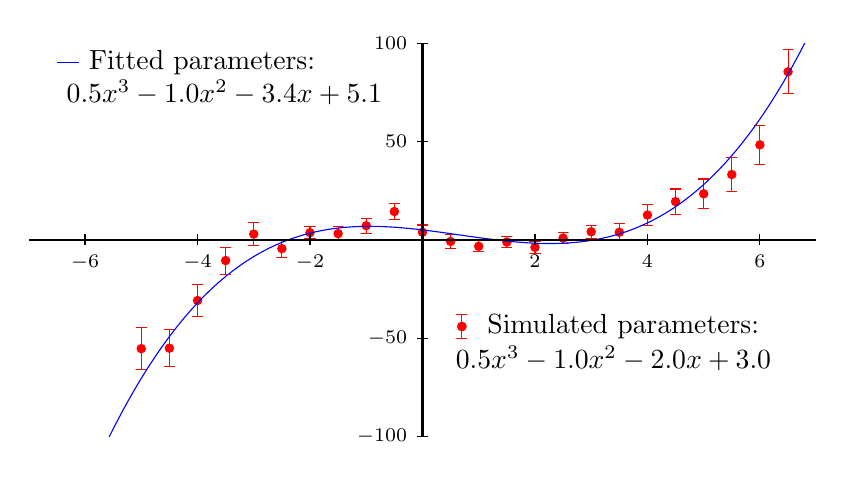
\begin{tikzpicture}
\begin{scope}[]
\pgfpathmoveto{ \pgfpointadd{\pgfpointxy {0.0} {0.0}} {\pgfpoint{0cm}{0cm}} }
\pgfpathlineto{ \pgfpointadd{\pgfpointxy {0.0} {0.0}} {\pgfpoint{10cm}{0cm}} }
\pgfpathlineto{ \pgfpointadd{\pgfpointxy {0.0} {0.0}} {\pgfpoint{10cm}{5cm}} }
\pgfpathlineto{ \pgfpointadd{\pgfpointxy {0.0} {0.0}} {\pgfpoint{0cm}{5cm}} }
\pgfpathclose
\pgfusepath{  clip, }
\begin{scope}[shift={(0.0,0.0)}]
\pgfsetxvec{\pgfpoint{0.71428573cm}{0cm}}
\pgfsetyvec{\pgfpoint{0cm}{0.025cm}}
\begin{scope}[shift={(7.0,100.0)}]
\begin{scope}[draw=red,fill=red]
\pgfpathmoveto{ \pgfpointadd{\pgfpointxy {-10.0} {-571.0535387380919}} {\pgfpoint{-2pt}{0}} }
\pgfpathlineto{ \pgfpointadd{\pgfpointxy {-10.0} {-571.0535387380919}} {\pgfpoint{2pt}{0}} }
\pgfpathlineto{ \pgfpointadd{\pgfpointxy {-10.0} {-571.0535387380919}} {\pgfpoint{0pt}{0}} }
\pgfpathlineto{ \pgfpointadd{\pgfpointxy {-10.0} {-623.095187335949}} {\pgfpoint{0pt}{0}} }
\pgfpathlineto{ \pgfpointadd{\pgfpointxy {-10.0} {-623.095187335949}} {\pgfpoint{-2pt}{0}} }
\pgfpathlineto{ \pgfpointadd{\pgfpointxy {-10.0} {-623.095187335949}} {\pgfpoint{2pt}{0}} }
\pgfusepath{ stroke, }
\node at (-10.0,-597.0743630370205) [draw=red,fill=red,circle,inner sep=0.0pt,minimum width =3.0pt,minimum height=3.0pt] {};
\end{scope}
\begin{scope}[draw=red,fill=red]
\pgfpathmoveto{ \pgfpointadd{\pgfpointxy {-9.5} {-465.4942843469761}} {\pgfpoint{-2pt}{0}} }
\pgfpathlineto{ \pgfpointadd{\pgfpointxy {-9.5} {-465.4942843469761}} {\pgfpoint{2pt}{0}} }
\pgfpathlineto{ \pgfpointadd{\pgfpointxy {-9.5} {-465.4942843469761}} {\pgfpoint{0pt}{0}} }
\pgfpathlineto{ \pgfpointadd{\pgfpointxy {-9.5} {-514.0784743698979}} {\pgfpoint{0pt}{0}} }
\pgfpathlineto{ \pgfpointadd{\pgfpointxy {-9.5} {-514.0784743698979}} {\pgfpoint{-2pt}{0}} }
\pgfpathlineto{ \pgfpointadd{\pgfpointxy {-9.5} {-514.0784743698979}} {\pgfpoint{2pt}{0}} }
\pgfusepath{ stroke, }
\node at (-9.5,-489.786379358437) [draw=red,fill=red,circle,inner sep=0.0pt,minimum width =3.0pt,minimum height=3.0pt] {};
\end{scope}
\begin{scope}[draw=red,fill=red]
\pgfpathmoveto{ \pgfpointadd{\pgfpointxy {-9.0} {-412.1044371552097}} {\pgfpoint{-2pt}{0}} }
\pgfpathlineto{ \pgfpointadd{\pgfpointxy {-9.0} {-412.1044371552097}} {\pgfpoint{2pt}{0}} }
\pgfpathlineto{ \pgfpointadd{\pgfpointxy {-9.0} {-412.1044371552097}} {\pgfpoint{0pt}{0}} }
\pgfpathlineto{ \pgfpointadd{\pgfpointxy {-9.0} {-457.3112327112828}} {\pgfpoint{0pt}{0}} }
\pgfpathlineto{ \pgfpointadd{\pgfpointxy {-9.0} {-457.3112327112828}} {\pgfpoint{-2pt}{0}} }
\pgfpathlineto{ \pgfpointadd{\pgfpointxy {-9.0} {-457.3112327112828}} {\pgfpoint{2pt}{0}} }
\pgfusepath{ stroke, }
\node at (-9.0,-434.70783493324626) [draw=red,fill=red,circle,inner sep=0.0pt,minimum width =3.0pt,minimum height=3.0pt] {};
\end{scope}
\begin{scope}[draw=red,fill=red]
\pgfpathmoveto{ \pgfpointadd{\pgfpointxy {-8.5} {-357.183759168102}} {\pgfpoint{-2pt}{0}} }
\pgfpathlineto{ \pgfpointadd{\pgfpointxy {-8.5} {-357.183759168102}} {\pgfpoint{2pt}{0}} }
\pgfpathlineto{ \pgfpointadd{\pgfpointxy {-8.5} {-357.183759168102}} {\pgfpoint{0pt}{0}} }
\pgfpathlineto{ \pgfpointadd{\pgfpointxy {-8.5} {-399.0948393426367}} {\pgfpoint{0pt}{0}} }
\pgfpathlineto{ \pgfpointadd{\pgfpointxy {-8.5} {-399.0948393426367}} {\pgfpoint{-2pt}{0}} }
\pgfpathlineto{ \pgfpointadd{\pgfpointxy {-8.5} {-399.0948393426367}} {\pgfpoint{2pt}{0}} }
\pgfusepath{ stroke, }
\node at (-8.5,-378.13929925536934) [draw=red,fill=red,circle,inner sep=0.0pt,minimum width =3.0pt,minimum height=3.0pt] {};
\end{scope}
\begin{scope}[draw=red,fill=red]
\pgfpathmoveto{ \pgfpointadd{\pgfpointxy {-8.0} {-291.87829172373085}} {\pgfpoint{-2pt}{0}} }
\pgfpathlineto{ \pgfpointadd{\pgfpointxy {-8.0} {-291.87829172373085}} {\pgfpoint{2pt}{0}} }
\pgfpathlineto{ \pgfpointadd{\pgfpointxy {-8.0} {-291.87829172373085}} {\pgfpoint{0pt}{0}} }
\pgfpathlineto{ \pgfpointadd{\pgfpointxy {-8.0} {-330.57699486952583}} {\pgfpoint{0pt}{0}} }
\pgfpathlineto{ \pgfpointadd{\pgfpointxy {-8.0} {-330.57699486952583}} {\pgfpoint{-2pt}{0}} }
\pgfpathlineto{ \pgfpointadd{\pgfpointxy {-8.0} {-330.57699486952583}} {\pgfpoint{2pt}{0}} }
\pgfusepath{ stroke, }
\node at (-8.0,-311.22764329662834) [draw=red,fill=red,circle,inner sep=0.0pt,minimum width =3.0pt,minimum height=3.0pt] {};
\end{scope}
\begin{scope}[draw=red,fill=red]
\pgfpathmoveto{ \pgfpointadd{\pgfpointxy {-7.5} {-238.3149428018001}} {\pgfpoint{-2pt}{0}} }
\pgfpathlineto{ \pgfpointadd{\pgfpointxy {-7.5} {-238.3149428018001}} {\pgfpoint{2pt}{0}} }
\pgfpathlineto{ \pgfpointadd{\pgfpointxy {-7.5} {-238.3149428018001}} {\pgfpoint{0pt}{0}} }
\pgfpathlineto{ \pgfpointadd{\pgfpointxy {-7.5} {-273.88629057157385}} {\pgfpoint{0pt}{0}} }
\pgfpathlineto{ \pgfpointadd{\pgfpointxy {-7.5} {-273.88629057157385}} {\pgfpoint{-2pt}{0}} }
\pgfpathlineto{ \pgfpointadd{\pgfpointxy {-7.5} {-273.88629057157385}} {\pgfpoint{2pt}{0}} }
\pgfusepath{ stroke, }
\node at (-7.5,-256.100616686687) [draw=red,fill=red,circle,inner sep=0.0pt,minimum width =3.0pt,minimum height=3.0pt] {};
\end{scope}
\begin{scope}[draw=red,fill=red]
\pgfpathmoveto{ \pgfpointadd{\pgfpointxy {-7.0} {-202.29808062975653}} {\pgfpoint{-2pt}{0}} }
\pgfpathlineto{ \pgfpointadd{\pgfpointxy {-7.0} {-202.29808062975653}} {\pgfpoint{2pt}{0}} }
\pgfpathlineto{ \pgfpointadd{\pgfpointxy {-7.0} {-202.29808062975653}} {\pgfpoint{0pt}{0}} }
\pgfpathlineto{ \pgfpointadd{\pgfpointxy {-7.0} {-234.82876586513075}} {\pgfpoint{0pt}{0}} }
\pgfpathlineto{ \pgfpointadd{\pgfpointxy {-7.0} {-234.82876586513075}} {\pgfpoint{-2pt}{0}} }
\pgfpathlineto{ \pgfpointadd{\pgfpointxy {-7.0} {-234.82876586513075}} {\pgfpoint{2pt}{0}} }
\pgfusepath{ stroke, }
\node at (-7.0,-218.56342324744364) [draw=red,fill=red,circle,inner sep=0.0pt,minimum width =3.0pt,minimum height=3.0pt] {};
\end{scope}
\begin{scope}[draw=red,fill=red]
\pgfpathmoveto{ \pgfpointadd{\pgfpointxy {-6.5} {-145.7322270733457}} {\pgfpoint{-2pt}{0}} }
\pgfpathlineto{ \pgfpointadd{\pgfpointxy {-6.5} {-145.7322270733457}} {\pgfpoint{2pt}{0}} }
\pgfpathlineto{ \pgfpointadd{\pgfpointxy {-6.5} {-145.7322270733457}} {\pgfpoint{0pt}{0}} }
\pgfpathlineto{ \pgfpointadd{\pgfpointxy {-6.5} {-175.31053819820306}} {\pgfpoint{0pt}{0}} }
\pgfpathlineto{ \pgfpointadd{\pgfpointxy {-6.5} {-175.31053819820306}} {\pgfpoint{-2pt}{0}} }
\pgfpathlineto{ \pgfpointadd{\pgfpointxy {-6.5} {-175.31053819820306}} {\pgfpoint{2pt}{0}} }
\pgfusepath{ stroke, }
\node at (-6.5,-160.5213826357744) [draw=red,fill=red,circle,inner sep=0.0pt,minimum width =3.0pt,minimum height=3.0pt] {};
\end{scope}
\begin{scope}[draw=red,fill=red]
\pgfpathmoveto{ \pgfpointadd{\pgfpointxy {-6.0} {-109.22115465709189}} {\pgfpoint{-2pt}{0}} }
\pgfpathlineto{ \pgfpointadd{\pgfpointxy {-6.0} {-109.22115465709189}} {\pgfpoint{2pt}{0}} }
\pgfpathlineto{ \pgfpointadd{\pgfpointxy {-6.0} {-109.22115465709189}} {\pgfpoint{0pt}{0}} }
\pgfpathlineto{ \pgfpointadd{\pgfpointxy {-6.0} {-135.93678804029298}} {\pgfpoint{0pt}{0}} }
\pgfpathlineto{ \pgfpointadd{\pgfpointxy {-6.0} {-135.93678804029298}} {\pgfpoint{-2pt}{0}} }
\pgfpathlineto{ \pgfpointadd{\pgfpointxy {-6.0} {-135.93678804029298}} {\pgfpoint{2pt}{0}} }
\pgfusepath{ stroke, }
\node at (-6.0,-122.57897134869243) [draw=red,fill=red,circle,inner sep=0.0pt,minimum width =3.0pt,minimum height=3.0pt] {};
\end{scope}
\begin{scope}[draw=red,fill=red]
\pgfpathmoveto{ \pgfpointadd{\pgfpointxy {-5.5} {-109.25232418508995}} {\pgfpoint{-2pt}{0}} }
\pgfpathlineto{ \pgfpointadd{\pgfpointxy {-5.5} {-109.25232418508995}} {\pgfpoint{2pt}{0}} }
\pgfpathlineto{ \pgfpointadd{\pgfpointxy {-5.5} {-109.25232418508995}} {\pgfpoint{0pt}{0}} }
\pgfpathlineto{ \pgfpointadd{\pgfpointxy {-5.5} {-133.19599486026908}} {\pgfpoint{0pt}{0}} }
\pgfpathlineto{ \pgfpointadd{\pgfpointxy {-5.5} {-133.19599486026908}} {\pgfpoint{-2pt}{0}} }
\pgfpathlineto{ \pgfpointadd{\pgfpointxy {-5.5} {-133.19599486026908}} {\pgfpoint{2pt}{0}} }
\pgfusepath{ stroke, }
\node at (-5.5,-121.22415952267951) [draw=red,fill=red,circle,inner sep=0.0pt,minimum width =3.0pt,minimum height=3.0pt] {};
\end{scope}
\begin{scope}[draw=red,fill=red]
\pgfpathmoveto{ \pgfpointadd{\pgfpointxy {-5.0} {-44.62018863682962}} {\pgfpoint{-2pt}{0}} }
\pgfpathlineto{ \pgfpointadd{\pgfpointxy {-5.0} {-44.62018863682962}} {\pgfpoint{2pt}{0}} }
\pgfpathlineto{ \pgfpointadd{\pgfpointxy {-5.0} {-44.62018863682962}} {\pgfpoint{0pt}{0}} }
\pgfpathlineto{ \pgfpointadd{\pgfpointxy {-5.0} {-65.88286513846168}} {\pgfpoint{0pt}{0}} }
\pgfpathlineto{ \pgfpointadd{\pgfpointxy {-5.0} {-65.88286513846168}} {\pgfpoint{-2pt}{0}} }
\pgfpathlineto{ \pgfpointadd{\pgfpointxy {-5.0} {-65.88286513846168}} {\pgfpoint{2pt}{0}} }
\pgfusepath{ stroke, }
\node at (-5.0,-55.25152688764565) [draw=red,fill=red,circle,inner sep=0.0pt,minimum width =3.0pt,minimum height=3.0pt] {};
\end{scope}
\begin{scope}[draw=red,fill=red]
\pgfpathmoveto{ \pgfpointadd{\pgfpointxy {-4.5} {-45.66786522760035}} {\pgfpoint{-2pt}{0}} }
\pgfpathlineto{ \pgfpointadd{\pgfpointxy {-4.5} {-45.66786522760035}} {\pgfpoint{2pt}{0}} }
\pgfpathlineto{ \pgfpointadd{\pgfpointxy {-4.5} {-45.66786522760035}} {\pgfpoint{0pt}{0}} }
\pgfpathlineto{ \pgfpointadd{\pgfpointxy {-4.5} {-64.33926597872156}} {\pgfpoint{0pt}{0}} }
\pgfpathlineto{ \pgfpointadd{\pgfpointxy {-4.5} {-64.33926597872156}} {\pgfpoint{-2pt}{0}} }
\pgfpathlineto{ \pgfpointadd{\pgfpointxy {-4.5} {-64.33926597872156}} {\pgfpoint{2pt}{0}} }
\pgfusepath{ stroke, }
\node at (-4.5,-55.00356560316096) [draw=red,fill=red,circle,inner sep=0.0pt,minimum width =3.0pt,minimum height=3.0pt] {};
\end{scope}
\begin{scope}[draw=red,fill=red]
\pgfpathmoveto{ \pgfpointadd{\pgfpointxy {-4.0} {-22.71518997590085}} {\pgfpoint{-2pt}{0}} }
\pgfpathlineto{ \pgfpointadd{\pgfpointxy {-4.0} {-22.71518997590085}} {\pgfpoint{2pt}{0}} }
\pgfpathlineto{ \pgfpointadd{\pgfpointxy {-4.0} {-22.71518997590085}} {\pgfpoint{0pt}{0}} }
\pgfpathlineto{ \pgfpointadd{\pgfpointxy {-4.0} {-38.880715036497286}} {\pgfpoint{0pt}{0}} }
\pgfpathlineto{ \pgfpointadd{\pgfpointxy {-4.0} {-38.880715036497286}} {\pgfpoint{-2pt}{0}} }
\pgfpathlineto{ \pgfpointadd{\pgfpointxy {-4.0} {-38.880715036497286}} {\pgfpoint{2pt}{0}} }
\pgfusepath{ stroke, }
\node at (-4.0,-30.797952506199067) [draw=red,fill=red,circle,inner sep=0.0pt,minimum width =3.0pt,minimum height=3.0pt] {};
\end{scope}
\begin{scope}[draw=red,fill=red]
\pgfpathmoveto{ \pgfpointadd{\pgfpointxy {-3.5} {-3.623367622026165}} {\pgfpoint{-2pt}{0}} }
\pgfpathlineto{ \pgfpointadd{\pgfpointxy {-3.5} {-3.623367622026165}} {\pgfpoint{2pt}{0}} }
\pgfpathlineto{ \pgfpointadd{\pgfpointxy {-3.5} {-3.623367622026165}} {\pgfpoint{0pt}{0}} }
\pgfpathlineto{ \pgfpointadd{\pgfpointxy {-3.5} {-17.357328788992056}} {\pgfpoint{0pt}{0}} }
\pgfpathlineto{ \pgfpointadd{\pgfpointxy {-3.5} {-17.357328788992056}} {\pgfpoint{-2pt}{0}} }
\pgfpathlineto{ \pgfpointadd{\pgfpointxy {-3.5} {-17.357328788992056}} {\pgfpoint{2pt}{0}} }
\pgfusepath{ stroke, }
\node at (-3.5,-10.490348205509111) [draw=red,fill=red,circle,inner sep=0.0pt,minimum width =3.0pt,minimum height=3.0pt] {};
\end{scope}
\begin{scope}[draw=red,fill=red]
\pgfpathmoveto{ \pgfpointadd{\pgfpointxy {-3.0} {8.659705441078653}} {\pgfpoint{-2pt}{0}} }
\pgfpathlineto{ \pgfpointadd{\pgfpointxy {-3.0} {8.659705441078653}} {\pgfpoint{2pt}{0}} }
\pgfpathlineto{ \pgfpointadd{\pgfpointxy {-3.0} {8.659705441078653}} {\pgfpoint{0pt}{0}} }
\pgfpathlineto{ \pgfpointadd{\pgfpointxy {-3.0} {-2.688763787270882}} {\pgfpoint{0pt}{0}} }
\pgfpathlineto{ \pgfpointadd{\pgfpointxy {-3.0} {-2.688763787270882}} {\pgfpoint{-2pt}{0}} }
\pgfpathlineto{ \pgfpointadd{\pgfpointxy {-3.0} {-2.688763787270882}} {\pgfpoint{2pt}{0}} }
\pgfusepath{ stroke, }
\node at (-3.0,2.985470826903885) [draw=red,fill=red,circle,inner sep=0.0pt,minimum width =3.0pt,minimum height=3.0pt] {};
\end{scope}
\begin{scope}[draw=red,fill=red]
\pgfpathmoveto{ \pgfpointadd{\pgfpointxy {-2.5} {0.03452070884278502}} {\pgfpoint{-2pt}{0}} }
\pgfpathlineto{ \pgfpointadd{\pgfpointxy {-2.5} {0.03452070884278502}} {\pgfpoint{2pt}{0}} }
\pgfpathlineto{ \pgfpointadd{\pgfpointxy {-2.5} {0.03452070884278502}} {\pgfpoint{0pt}{0}} }
\pgfpathlineto{ \pgfpointadd{\pgfpointxy {-2.5} {-8.889908192055266}} {\pgfpoint{0pt}{0}} }
\pgfpathlineto{ \pgfpointadd{\pgfpointxy {-2.5} {-8.889908192055266}} {\pgfpoint{-2pt}{0}} }
\pgfpathlineto{ \pgfpointadd{\pgfpointxy {-2.5} {-8.889908192055266}} {\pgfpoint{2pt}{0}} }
\pgfusepath{ stroke, }
\node at (-2.5,-4.427693741606241) [draw=red,fill=red,circle,inner sep=0.0pt,minimum width =3.0pt,minimum height=3.0pt] {};
\end{scope}
\begin{scope}[draw=red,fill=red]
\pgfpathmoveto{ \pgfpointadd{\pgfpointxy {-2.0} {6.691469768324479}} {\pgfpoint{-2pt}{0}} }
\pgfpathlineto{ \pgfpointadd{\pgfpointxy {-2.0} {6.691469768324479}} {\pgfpoint{2pt}{0}} }
\pgfpathlineto{ \pgfpointadd{\pgfpointxy {-2.0} {6.691469768324479}} {\pgfpoint{0pt}{0}} }
\pgfpathlineto{ \pgfpointadd{\pgfpointxy {-2.0} {0.6914697683244793}} {\pgfpoint{0pt}{0}} }
\pgfpathlineto{ \pgfpointadd{\pgfpointxy {-2.0} {0.6914697683244793}} {\pgfpoint{-2pt}{0}} }
\pgfpathlineto{ \pgfpointadd{\pgfpointxy {-2.0} {0.6914697683244793}} {\pgfpoint{2pt}{0}} }
\pgfusepath{ stroke, }
\node at (-2.0,3.6914697683244793) [draw=red,fill=red,circle,inner sep=0.0pt,minimum width =3.0pt,minimum height=3.0pt] {};
\end{scope}
\begin{scope}[draw=red,fill=red]
\pgfpathmoveto{ \pgfpointadd{\pgfpointxy {-1.5} {6.642849316210677}} {\pgfpoint{-2pt}{0}} }
\pgfpathlineto{ \pgfpointadd{\pgfpointxy {-1.5} {6.642849316210677}} {\pgfpoint{2pt}{0}} }
\pgfpathlineto{ \pgfpointadd{\pgfpointxy {-1.5} {6.642849316210677}} {\pgfpoint{0pt}{0}} }
\pgfpathlineto{ \pgfpointadd{\pgfpointxy {-1.5} {-0.2294320070583371}} {\pgfpoint{0pt}{0}} }
\pgfpathlineto{ \pgfpointadd{\pgfpointxy {-1.5} {-0.2294320070583371}} {\pgfpoint{-2pt}{0}} }
\pgfpathlineto{ \pgfpointadd{\pgfpointxy {-1.5} {-0.2294320070583371}} {\pgfpoint{2pt}{0}} }
\pgfusepath{ stroke, }
\node at (-1.5,3.20670865457617) [draw=red,fill=red,circle,inner sep=0.0pt,minimum width =3.0pt,minimum height=3.0pt] {};
\end{scope}
\begin{scope}[draw=red,fill=red]
\pgfpathmoveto{ \pgfpointadd{\pgfpointxy {-1.0} {11.107898214064939}} {\pgfpoint{-2pt}{0}} }
\pgfpathlineto{ \pgfpointadd{\pgfpointxy {-1.0} {11.107898214064939}} {\pgfpoint{2pt}{0}} }
\pgfpathlineto{ \pgfpointadd{\pgfpointxy {-1.0} {11.107898214064939}} {\pgfpoint{0pt}{0}} }
\pgfpathlineto{ \pgfpointadd{\pgfpointxy {-1.0} {3.3662408272909987}} {\pgfpoint{0pt}{0}} }
\pgfpathlineto{ \pgfpointadd{\pgfpointxy {-1.0} {3.3662408272909987}} {\pgfpoint{-2pt}{0}} }
\pgfpathlineto{ \pgfpointadd{\pgfpointxy {-1.0} {3.3662408272909987}} {\pgfpoint{2pt}{0}} }
\pgfusepath{ stroke, }
\node at (-1.0,7.237069520677969) [draw=red,fill=red,circle,inner sep=0.0pt,minimum width =3.0pt,minimum height=3.0pt] {};
\end{scope}
\begin{scope}[draw=red,fill=red]
\pgfpathmoveto{ \pgfpointadd{\pgfpointxy {-0.5} {18.362804815403905}} {\pgfpoint{-2pt}{0}} }
\pgfpathlineto{ \pgfpointadd{\pgfpointxy {-0.5} {18.362804815403905}} {\pgfpoint{2pt}{0}} }
\pgfpathlineto{ \pgfpointadd{\pgfpointxy {-0.5} {18.362804815403905}} {\pgfpoint{0pt}{0}} }
\pgfpathlineto{ \pgfpointadd{\pgfpointxy {-0.5} {10.522231941469602}} {\pgfpoint{0pt}{0}} }
\pgfpathlineto{ \pgfpointadd{\pgfpointxy {-0.5} {10.522231941469602}} {\pgfpoint{-2pt}{0}} }
\pgfpathlineto{ \pgfpointadd{\pgfpointxy {-0.5} {10.522231941469602}} {\pgfpoint{2pt}{0}} }
\pgfusepath{ stroke, }
\node at (-0.5,14.442518378436754) [draw=red,fill=red,circle,inner sep=0.0pt,minimum width =3.0pt,minimum height=3.0pt] {};
\end{scope}
\begin{scope}[draw=red,fill=red]
\pgfpathmoveto{ \pgfpointadd{\pgfpointxy {0.0} {7.612007955975413}} {\pgfpoint{-2pt}{0}} }
\pgfpathlineto{ \pgfpointadd{\pgfpointxy {0.0} {7.612007955975413}} {\pgfpoint{2pt}{0}} }
\pgfpathlineto{ \pgfpointadd{\pgfpointxy {0.0} {7.612007955975413}} {\pgfpoint{0pt}{0}} }
\pgfpathlineto{ \pgfpointadd{\pgfpointxy {0.0} {0.14790634083765797}} {\pgfpoint{0pt}{0}} }
\pgfpathlineto{ \pgfpointadd{\pgfpointxy {0.0} {0.14790634083765797}} {\pgfpoint{-2pt}{0}} }
\pgfpathlineto{ \pgfpointadd{\pgfpointxy {0.0} {0.14790634083765797}} {\pgfpoint{2pt}{0}} }
\pgfusepath{ stroke, }
\node at (0.0,3.879957148406535) [draw=red,fill=red,circle,inner sep=0.0pt,minimum width =3.0pt,minimum height=3.0pt] {};
\end{scope}
\begin{scope}[draw=red,fill=red]
\pgfpathmoveto{ \pgfpointadd{\pgfpointxy {0.5} {2.5683907793851475}} {\pgfpoint{-2pt}{0}} }
\pgfpathlineto{ \pgfpointadd{\pgfpointxy {0.5} {2.5683907793851475}} {\pgfpoint{2pt}{0}} }
\pgfpathlineto{ \pgfpointadd{\pgfpointxy {0.5} {2.5683907793851475}} {\pgfpoint{0pt}{0}} }
\pgfpathlineto{ \pgfpointadd{\pgfpointxy {0.5} {-4.124191624182105}} {\pgfpoint{0pt}{0}} }
\pgfpathlineto{ \pgfpointadd{\pgfpointxy {0.5} {-4.124191624182105}} {\pgfpoint{-2pt}{0}} }
\pgfpathlineto{ \pgfpointadd{\pgfpointxy {0.5} {-4.124191624182105}} {\pgfpoint{2pt}{0}} }
\pgfusepath{ stroke, }
\node at (0.5,-0.7779004223984787) [draw=red,fill=red,circle,inner sep=0.0pt,minimum width =3.0pt,minimum height=3.0pt] {};
\end{scope}
\begin{scope}[draw=red,fill=red]
\pgfpathmoveto{ \pgfpointadd{\pgfpointxy {1.0} {-0.5092360123617312}} {\pgfpoint{-2pt}{0}} }
\pgfpathlineto{ \pgfpointadd{\pgfpointxy {1.0} {-0.5092360123617312}} {\pgfpoint{2pt}{0}} }
\pgfpathlineto{ \pgfpointadd{\pgfpointxy {1.0} {-0.5092360123617312}} {\pgfpoint{0pt}{0}} }
\pgfpathlineto{ \pgfpointadd{\pgfpointxy {1.0} {-5.923449574734827}} {\pgfpoint{0pt}{0}} }
\pgfpathlineto{ \pgfpointadd{\pgfpointxy {1.0} {-5.923449574734827}} {\pgfpoint{-2pt}{0}} }
\pgfpathlineto{ \pgfpointadd{\pgfpointxy {1.0} {-5.923449574734827}} {\pgfpoint{2pt}{0}} }
\pgfusepath{ stroke, }
\node at (1.0,-3.2163427935482787) [draw=red,fill=red,circle,inner sep=0.0pt,minimum width =3.0pt,minimum height=3.0pt] {};
\end{scope}
\begin{scope}[draw=red,fill=red]
\pgfpathmoveto{ \pgfpointadd{\pgfpointxy {1.5} {1.6701722960789132}} {\pgfpoint{-2pt}{0}} }
\pgfpathlineto{ \pgfpointadd{\pgfpointxy {1.5} {1.6701722960789132}} {\pgfpoint{2pt}{0}} }
\pgfpathlineto{ \pgfpointadd{\pgfpointxy {1.5} {1.6701722960789132}} {\pgfpoint{0pt}{0}} }
\pgfpathlineto{ \pgfpointadd{\pgfpointxy {1.5} {-3.8298277039210866}} {\pgfpoint{0pt}{0}} }
\pgfpathlineto{ \pgfpointadd{\pgfpointxy {1.5} {-3.8298277039210866}} {\pgfpoint{-2pt}{0}} }
\pgfpathlineto{ \pgfpointadd{\pgfpointxy {1.5} {-3.8298277039210866}} {\pgfpoint{2pt}{0}} }
\pgfusepath{ stroke, }
\node at (1.5,-1.0798277039210868) [draw=red,fill=red,circle,inner sep=0.0pt,minimum width =3.0pt,minimum height=3.0pt] {};
\end{scope}
\begin{scope}[draw=red,fill=red]
\pgfpathmoveto{ \pgfpointadd{\pgfpointxy {2.0} {-0.7755617046804377}} {\pgfpoint{-2pt}{0}} }
\pgfpathlineto{ \pgfpointadd{\pgfpointxy {2.0} {-0.7755617046804377}} {\pgfpoint{2pt}{0}} }
\pgfpathlineto{ \pgfpointadd{\pgfpointxy {2.0} {-0.7755617046804377}} {\pgfpoint{0pt}{0}} }
\pgfpathlineto{ \pgfpointadd{\pgfpointxy {2.0} {-6.775561704680438}} {\pgfpoint{0pt}{0}} }
\pgfpathlineto{ \pgfpointadd{\pgfpointxy {2.0} {-6.775561704680438}} {\pgfpoint{-2pt}{0}} }
\pgfpathlineto{ \pgfpointadd{\pgfpointxy {2.0} {-6.775561704680438}} {\pgfpoint{2pt}{0}} }
\pgfusepath{ stroke, }
\node at (2.0,-3.7755617046804377) [draw=red,fill=red,circle,inner sep=0.0pt,minimum width =3.0pt,minimum height=3.0pt] {};
\end{scope}
\begin{scope}[draw=red,fill=red]
\pgfpathmoveto{ \pgfpointadd{\pgfpointxy {2.5} {3.599233927702615}} {\pgfpoint{-2pt}{0}} }
\pgfpathlineto{ \pgfpointadd{\pgfpointxy {2.5} {3.599233927702615}} {\pgfpoint{2pt}{0}} }
\pgfpathlineto{ \pgfpointadd{\pgfpointxy {2.5} {3.599233927702615}} {\pgfpoint{0pt}{0}} }
\pgfpathlineto{ \pgfpointadd{\pgfpointxy {2.5} {-1.72364172782968}} {\pgfpoint{0pt}{0}} }
\pgfpathlineto{ \pgfpointadd{\pgfpointxy {2.5} {-1.72364172782968}} {\pgfpoint{-2pt}{0}} }
\pgfpathlineto{ \pgfpointadd{\pgfpointxy {2.5} {-1.72364172782968}} {\pgfpoint{2pt}{0}} }
\pgfusepath{ stroke, }
\node at (2.5,0.9377960999364674) [draw=red,fill=red,circle,inner sep=0.0pt,minimum width =3.0pt,minimum height=3.0pt] {};
\end{scope}
\begin{scope}[draw=red,fill=red]
\pgfpathmoveto{ \pgfpointadd{\pgfpointxy {3.0} {7.3753525624062775}} {\pgfpoint{-2pt}{0}} }
\pgfpathlineto{ \pgfpointadd{\pgfpointxy {3.0} {7.3753525624062775}} {\pgfpoint{2pt}{0}} }
\pgfpathlineto{ \pgfpointadd{\pgfpointxy {3.0} {7.3753525624062775}} {\pgfpoint{0pt}{0}} }
\pgfpathlineto{ \pgfpointadd{\pgfpointxy {3.0} {0.9258628196231}} {\pgfpoint{0pt}{0}} }
\pgfpathlineto{ \pgfpointadd{\pgfpointxy {3.0} {0.9258628196231}} {\pgfpoint{-2pt}{0}} }
\pgfpathlineto{ \pgfpointadd{\pgfpointxy {3.0} {0.9258628196231}} {\pgfpoint{2pt}{0}} }
\pgfusepath{ stroke, }
\node at (3.0,4.150607691014689) [draw=red,fill=red,circle,inner sep=0.0pt,minimum width =3.0pt,minimum height=3.0pt] {};
\end{scope}
\begin{scope}[draw=red,fill=red]
\pgfpathmoveto{ \pgfpointadd{\pgfpointxy {3.5} {8.180402037547292}} {\pgfpoint{-2pt}{0}} }
\pgfpathlineto{ \pgfpointadd{\pgfpointxy {3.5} {8.180402037547292}} {\pgfpoint{2pt}{0}} }
\pgfpathlineto{ \pgfpointadd{\pgfpointxy {3.5} {8.180402037547292}} {\pgfpoint{0pt}{0}} }
\pgfpathlineto{ \pgfpointadd{\pgfpointxy {3.5} {-0.37481475202485726}} {\pgfpoint{0pt}{0}} }
\pgfpathlineto{ \pgfpointadd{\pgfpointxy {3.5} {-0.37481475202485726}} {\pgfpoint{-2pt}{0}} }
\pgfpathlineto{ \pgfpointadd{\pgfpointxy {3.5} {-0.37481475202485726}} {\pgfpoint{2pt}{0}} }
\pgfusepath{ stroke, }
\node at (3.5,3.9027936427612175) [draw=red,fill=red,circle,inner sep=0.0pt,minimum width =3.0pt,minimum height=3.0pt] {};
\end{scope}
\begin{scope}[draw=red,fill=red]
\pgfpathmoveto{ \pgfpointadd{\pgfpointxy {4.0} {17.985284457749778}} {\pgfpoint{-2pt}{0}} }
\pgfpathlineto{ \pgfpointadd{\pgfpointxy {4.0} {17.985284457749778}} {\pgfpoint{2pt}{0}} }
\pgfpathlineto{ \pgfpointadd{\pgfpointxy {4.0} {17.985284457749778}} {\pgfpoint{0pt}{0}} }
\pgfpathlineto{ \pgfpointadd{\pgfpointxy {4.0} {7.352034877038976}} {\pgfpoint{0pt}{0}} }
\pgfpathlineto{ \pgfpointadd{\pgfpointxy {4.0} {7.352034877038976}} {\pgfpoint{-2pt}{0}} }
\pgfpathlineto{ \pgfpointadd{\pgfpointxy {4.0} {7.352034877038976}} {\pgfpoint{2pt}{0}} }
\pgfusepath{ stroke, }
\node at (4.0,12.668659667394376) [draw=red,fill=red,circle,inner sep=0.0pt,minimum width =3.0pt,minimum height=3.0pt] {};
\end{scope}
\begin{scope}[draw=red,fill=red]
\pgfpathmoveto{ \pgfpointadd{\pgfpointxy {4.5} {25.865344976413038}} {\pgfpoint{-2pt}{0}} }
\pgfpathlineto{ \pgfpointadd{\pgfpointxy {4.5} {25.865344976413038}} {\pgfpoint{2pt}{0}} }
\pgfpathlineto{ \pgfpointadd{\pgfpointxy {4.5} {25.865344976413038}} {\pgfpoint{0pt}{0}} }
\pgfpathlineto{ \pgfpointadd{\pgfpointxy {4.5} {13.076147060789562}} {\pgfpoint{0pt}{0}} }
\pgfpathlineto{ \pgfpointadd{\pgfpointxy {4.5} {13.076147060789562}} {\pgfpoint{-2pt}{0}} }
\pgfpathlineto{ \pgfpointadd{\pgfpointxy {4.5} {13.076147060789562}} {\pgfpoint{2pt}{0}} }
\pgfusepath{ stroke, }
\node at (4.5,19.4707460186013) [draw=red,fill=red,circle,inner sep=0.0pt,minimum width =3.0pt,minimum height=3.0pt] {};
\end{scope}
\begin{scope}[draw=red,fill=red]
\pgfpathmoveto{ \pgfpointadd{\pgfpointxy {5.0} {30.966184447206345}} {\pgfpoint{-2pt}{0}} }
\pgfpathlineto{ \pgfpointadd{\pgfpointxy {5.0} {30.966184447206345}} {\pgfpoint{2pt}{0}} }
\pgfpathlineto{ \pgfpointadd{\pgfpointxy {5.0} {30.966184447206345}} {\pgfpoint{0pt}{0}} }
\pgfpathlineto{ \pgfpointadd{\pgfpointxy {5.0} {15.920823430019084}} {\pgfpoint{0pt}{0}} }
\pgfpathlineto{ \pgfpointadd{\pgfpointxy {5.0} {15.920823430019084}} {\pgfpoint{-2pt}{0}} }
\pgfpathlineto{ \pgfpointadd{\pgfpointxy {5.0} {15.920823430019084}} {\pgfpoint{2pt}{0}} }
\pgfusepath{ stroke, }
\node at (5.0,23.443503938612714) [draw=red,fill=red,circle,inner sep=0.0pt,minimum width =3.0pt,minimum height=3.0pt] {};
\end{scope}
\begin{scope}[draw=red,fill=red]
\pgfpathmoveto{ \pgfpointadd{\pgfpointxy {5.5} {41.93279338298936}} {\pgfpoint{-2pt}{0}} }
\pgfpathlineto{ \pgfpointadd{\pgfpointxy {5.5} {41.93279338298936}} {\pgfpoint{2pt}{0}} }
\pgfpathlineto{ \pgfpointadd{\pgfpointxy {5.5} {41.93279338298936}} {\pgfpoint{0pt}{0}} }
\pgfpathlineto{ \pgfpointadd{\pgfpointxy {5.5} {24.52570570519744}} {\pgfpoint{0pt}{0}} }
\pgfpathlineto{ \pgfpointadd{\pgfpointxy {5.5} {24.52570570519744}} {\pgfpoint{-2pt}{0}} }
\pgfpathlineto{ \pgfpointadd{\pgfpointxy {5.5} {24.52570570519744}} {\pgfpoint{2pt}{0}} }
\pgfusepath{ stroke, }
\node at (5.5,33.2292495440934) [draw=red,fill=red,circle,inner sep=0.0pt,minimum width =3.0pt,minimum height=3.0pt] {};
\end{scope}
\begin{scope}[draw=red,fill=red]
\pgfpathmoveto{ \pgfpointadd{\pgfpointxy {6.0} {58.24963967593858}} {\pgfpoint{-2pt}{0}} }
\pgfpathlineto{ \pgfpointadd{\pgfpointxy {6.0} {58.24963967593858}} {\pgfpoint{2pt}{0}} }
\pgfpathlineto{ \pgfpointadd{\pgfpointxy {6.0} {58.24963967593858}} {\pgfpoint{0pt}{0}} }
\pgfpathlineto{ \pgfpointadd{\pgfpointxy {6.0} {38.375131809551036}} {\pgfpoint{0pt}{0}} }
\pgfpathlineto{ \pgfpointadd{\pgfpointxy {6.0} {38.375131809551036}} {\pgfpoint{-2pt}{0}} }
\pgfpathlineto{ \pgfpointadd{\pgfpointxy {6.0} {38.375131809551036}} {\pgfpoint{2pt}{0}} }
\pgfusepath{ stroke, }
\node at (6.0,48.31238574274481) [draw=red,fill=red,circle,inner sep=0.0pt,minimum width =3.0pt,minimum height=3.0pt] {};
\end{scope}
\begin{scope}[draw=red,fill=red]
\pgfpathmoveto{ \pgfpointadd{\pgfpointxy {6.5} {96.67541812918063}} {\pgfpoint{-2pt}{0}} }
\pgfpathlineto{ \pgfpointadd{\pgfpointxy {6.5} {96.67541812918063}} {\pgfpoint{2pt}{0}} }
\pgfpathlineto{ \pgfpointadd{\pgfpointxy {6.5} {96.67541812918063}} {\pgfpoint{0pt}{0}} }
\pgfpathlineto{ \pgfpointadd{\pgfpointxy {6.5} {74.22955138348391}} {\pgfpoint{0pt}{0}} }
\pgfpathlineto{ \pgfpointadd{\pgfpointxy {6.5} {74.22955138348391}} {\pgfpoint{-2pt}{0}} }
\pgfpathlineto{ \pgfpointadd{\pgfpointxy {6.5} {74.22955138348391}} {\pgfpoint{2pt}{0}} }
\pgfusepath{ stroke, }
\node at (6.5,85.45248475633227) [draw=red,fill=red,circle,inner sep=0.0pt,minimum width =3.0pt,minimum height=3.0pt] {};
\end{scope}
\begin{scope}[draw=red,fill=red]
\pgfpathmoveto{ \pgfpointadd{\pgfpointxy {7.0} {150.98758050732656}} {\pgfpoint{-2pt}{0}} }
\pgfpathlineto{ \pgfpointadd{\pgfpointxy {7.0} {150.98758050732656}} {\pgfpoint{2pt}{0}} }
\pgfpathlineto{ \pgfpointadd{\pgfpointxy {7.0} {150.98758050732656}} {\pgfpoint{0pt}{0}} }
\pgfpathlineto{ \pgfpointadd{\pgfpointxy {7.0} {125.86886842538368}} {\pgfpoint{0pt}{0}} }
\pgfpathlineto{ \pgfpointadd{\pgfpointxy {7.0} {125.86886842538368}} {\pgfpoint{-2pt}{0}} }
\pgfpathlineto{ \pgfpointadd{\pgfpointxy {7.0} {125.86886842538368}} {\pgfpoint{2pt}{0}} }
\pgfusepath{ stroke, }
\node at (7.0,138.42822446635512) [draw=red,fill=red,circle,inner sep=0.0pt,minimum width =3.0pt,minimum height=3.0pt] {};
\end{scope}
\begin{scope}[draw=red,fill=red]
\pgfpathmoveto{ \pgfpointadd{\pgfpointxy {7.5} {137.62912541707732}} {\pgfpoint{-2pt}{0}} }
\pgfpathlineto{ \pgfpointadd{\pgfpointxy {7.5} {137.62912541707732}} {\pgfpoint{2pt}{0}} }
\pgfpathlineto{ \pgfpointadd{\pgfpointxy {7.5} {137.62912541707732}} {\pgfpoint{0pt}{0}} }
\pgfpathlineto{ \pgfpointadd{\pgfpointxy {7.5} {109.73875078627674}} {\pgfpoint{0pt}{0}} }
\pgfpathlineto{ \pgfpointadd{\pgfpointxy {7.5} {109.73875078627674}} {\pgfpoint{-2pt}{0}} }
\pgfpathlineto{ \pgfpointadd{\pgfpointxy {7.5} {109.73875078627674}} {\pgfpoint{2pt}{0}} }
\pgfusepath{ stroke, }
\node at (7.5,123.68393810167703) [draw=red,fill=red,circle,inner sep=0.0pt,minimum width =3.0pt,minimum height=3.0pt] {};
\end{scope}
\begin{scope}[draw=red,fill=red]
\pgfpathmoveto{ \pgfpointadd{\pgfpointxy {8.0} {201.411347251231}} {\pgfpoint{-2pt}{0}} }
\pgfpathlineto{ \pgfpointadd{\pgfpointxy {8.0} {201.411347251231}} {\pgfpoint{2pt}{0}} }
\pgfpathlineto{ \pgfpointadd{\pgfpointxy {8.0} {201.411347251231}} {\pgfpoint{0pt}{0}} }
\pgfpathlineto{ \pgfpointadd{\pgfpointxy {8.0} {170.65317093071172}} {\pgfpoint{0pt}{0}} }
\pgfpathlineto{ \pgfpointadd{\pgfpointxy {8.0} {170.65317093071172}} {\pgfpoint{-2pt}{0}} }
\pgfpathlineto{ \pgfpointadd{\pgfpointxy {8.0} {170.65317093071172}} {\pgfpoint{2pt}{0}} }
\pgfusepath{ stroke, }
\node at (8.0,186.03225909097137) [draw=red,fill=red,circle,inner sep=0.0pt,minimum width =3.0pt,minimum height=3.0pt] {};
\end{scope}
\begin{scope}[draw=red,fill=red]
\pgfpathmoveto{ \pgfpointadd{\pgfpointxy {8.5} {240.7691872656242}} {\pgfpoint{-2pt}{0}} }
\pgfpathlineto{ \pgfpointadd{\pgfpointxy {8.5} {240.7691872656242}} {\pgfpoint{2pt}{0}} }
\pgfpathlineto{ \pgfpointadd{\pgfpointxy {8.5} {240.7691872656242}} {\pgfpoint{0pt}{0}} }
\pgfpathlineto{ \pgfpointadd{\pgfpointxy {8.5} {207.04966506219702}} {\pgfpoint{0pt}{0}} }
\pgfpathlineto{ \pgfpointadd{\pgfpointxy {8.5} {207.04966506219702}} {\pgfpoint{-2pt}{0}} }
\pgfpathlineto{ \pgfpointadd{\pgfpointxy {8.5} {207.04966506219702}} {\pgfpoint{2pt}{0}} }
\pgfusepath{ stroke, }
\node at (8.5,223.9094261639106) [draw=red,fill=red,circle,inner sep=0.0pt,minimum width =3.0pt,minimum height=3.0pt] {};
\end{scope}
\begin{scope}[draw=red,fill=red]
\pgfpathmoveto{ \pgfpointadd{\pgfpointxy {9.0} {309.16018045080494}} {\pgfpoint{-2pt}{0}} }
\pgfpathlineto{ \pgfpointadd{\pgfpointxy {9.0} {309.16018045080494}} {\pgfpoint{2pt}{0}} }
\pgfpathlineto{ \pgfpointadd{\pgfpointxy {9.0} {309.16018045080494}} {\pgfpoint{0pt}{0}} }
\pgfpathlineto{ \pgfpointadd{\pgfpointxy {9.0} {272.3882412344571}} {\pgfpoint{0pt}{0}} }
\pgfpathlineto{ \pgfpointadd{\pgfpointxy {9.0} {272.3882412344571}} {\pgfpoint{-2pt}{0}} }
\pgfpathlineto{ \pgfpointadd{\pgfpointxy {9.0} {272.3882412344571}} {\pgfpoint{2pt}{0}} }
\pgfusepath{ stroke, }
\node at (9.0,290.774210842631) [draw=red,fill=red,circle,inner sep=0.0pt,minimum width =3.0pt,minimum height=3.0pt] {};
\end{scope}
\begin{scope}[draw=red,fill=red]
\pgfpathmoveto{ \pgfpointadd{\pgfpointxy {9.5} {335.072764831252}} {\pgfpoint{-2pt}{0}} }
\pgfpathlineto{ \pgfpointadd{\pgfpointxy {9.5} {335.072764831252}} {\pgfpoint{2pt}{0}} }
\pgfpathlineto{ \pgfpointadd{\pgfpointxy {9.5} {335.072764831252}} {\pgfpoint{0pt}{0}} }
\pgfpathlineto{ \pgfpointadd{\pgfpointxy {9.5} {295.159675295541}} {\pgfpoint{0pt}{0}} }
\pgfpathlineto{ \pgfpointadd{\pgfpointxy {9.5} {295.159675295541}} {\pgfpoint{-2pt}{0}} }
\pgfpathlineto{ \pgfpointadd{\pgfpointxy {9.5} {295.159675295541}} {\pgfpoint{2pt}{0}} }
\pgfusepath{ stroke, }
\node at (9.5,315.1162200633965) [draw=red,fill=red,circle,inner sep=0.0pt,minimum width =3.0pt,minimum height=3.0pt] {};
\end{scope}
\begin{scope}[draw=red,fill=red]
\pgfpathmoveto{ \pgfpointadd{\pgfpointxy {10.0} {419.00919636744237}} {\pgfpoint{-2pt}{0}} }
\pgfpathlineto{ \pgfpointadd{\pgfpointxy {10.0} {419.00919636744237}} {\pgfpoint{2pt}{0}} }
\pgfpathlineto{ \pgfpointadd{\pgfpointxy {10.0} {419.00919636744237}} {\pgfpoint{0pt}{0}} }
\pgfpathlineto{ \pgfpointadd{\pgfpointxy {10.0} {375.86842478588056}} {\pgfpoint{0pt}{0}} }
\pgfpathlineto{ \pgfpointadd{\pgfpointxy {10.0} {375.86842478588056}} {\pgfpoint{-2pt}{0}} }
\pgfpathlineto{ \pgfpointadd{\pgfpointxy {10.0} {375.86842478588056}} {\pgfpoint{2pt}{0}} }
\pgfusepath{ stroke, }
\node at (10.0,397.43881057666147) [draw=red,fill=red,circle,inner sep=0.0pt,minimum width =3.0pt,minimum height=3.0pt] {};
\end{scope}
\end{scope}
\pgfsetxvec{\pgfpoint{1cm}{0cm}}
\pgfsetyvec{\pgfpoint{0cm}{1cm}}
\end{scope}
\end{scope}
\begin{scope}[draw=red,fill=red]
\pgfpathmoveto{ \pgfpointadd{\pgfpointxy {5.5} {1.55}} {\pgfpoint{-2pt}{0}} }
\pgfpathlineto{ \pgfpointadd{\pgfpointxy {5.5} {1.55}} {\pgfpoint{2pt}{0}} }
\pgfpathlineto{ \pgfpointadd{\pgfpointxy {5.5} {1.55}} {\pgfpoint{0pt}{0}} }
\pgfpathlineto{ \pgfpointadd{\pgfpointxy {5.5} {1.25}} {\pgfpoint{0pt}{0}} }
\pgfpathlineto{ \pgfpointadd{\pgfpointxy {5.5} {1.25}} {\pgfpoint{-2pt}{0}} }
\pgfpathlineto{ \pgfpointadd{\pgfpointxy {5.5} {1.25}} {\pgfpoint{2pt}{0}} }
\pgfusepath{ stroke, }
\node at (5.5,1.4) [draw=red,fill=red,circle,inner sep=0.0pt,minimum width =3.0pt,minimum height=3.0pt] {};
\end{scope}
\node at (5.5,1.4) [draw=red,fill=red,circle,inner sep=0.0pt,minimum width =3.0pt,minimum height=3.0pt] {};
\node at (5.7000003,1.4) [right,,] {Simulated parameters:};
\node at (5.3,1.0) [right,] {$0.5x^3 -1.0x^2 -2.0x +3.0$};
\begin{scope}[shift={(0.0,0.0)}]
\pgfsetxvec{\pgfpoint{0.71428573cm}{0cm}}
\pgfsetyvec{\pgfpoint{0cm}{0.025cm}}
\begin{scope}[shift={(7.0,100.0)}]
\begin{scope}[]
\pgfpathmoveto{ \pgfpointadd{\pgfpointxy {-7.0} {-100.0}} {\pgfpoint{0cm}{0cm}} }
\pgfpathlineto{ \pgfpointadd{\pgfpointxy {-7.0} {-100.0}} {\pgfpoint{10cm}{0cm}} }
\pgfpathlineto{ \pgfpointadd{\pgfpointxy {-7.0} {-100.0}} {\pgfpoint{10cm}{5cm}} }
\pgfpathlineto{ \pgfpointadd{\pgfpointxy {-7.0} {-100.0}} {\pgfpoint{0cm}{5cm}} }
\pgfpathclose
\pgfusepath{  clip, }
\begin{scope}[blue]
\pgfpathmoveto{ \pgfpointxy {-7.0} {-204.1833528661588}}
\pgfpathlineto{ \pgfpointxy {-6.93} {-198.0023051665342}}
\pgfpathlineto{ \pgfpointxy {-6.86} {-191.93947097931303}}
\pgfpathlineto{ \pgfpointxy {-6.79} {-185.99375987479632}}
\pgfpathlineto{ \pgfpointxy {-6.72} {-180.16408142328484}}
\pgfpathlineto{ \pgfpointxy {-6.65} {-174.4493451950795}}
\pgfpathlineto{ \pgfpointxy {-6.58} {-168.84846076048117}}
\pgfpathlineto{ \pgfpointxy {-6.51} {-163.36033768979075}}
\pgfpathlineto{ \pgfpointxy {-6.44} {-157.9838855533091}}
\pgfpathlineto{ \pgfpointxy {-6.37} {-152.71801392133716}}
\pgfpathlineto{ \pgfpointxy {-6.3} {-147.56163236417572}}
\pgfpathlineto{ \pgfpointxy {-6.23} {-142.5136504521258}}
\pgfpathlineto{ \pgfpointxy {-6.16} {-137.57297775548813}}
\pgfpathlineto{ \pgfpointxy {-6.09} {-132.73852384456367}}
\pgfpathlineto{ \pgfpointxy {-6.02} {-128.00919828965326}}
\pgfpathlineto{ \pgfpointxy {-5.95} {-123.38391066105784}}
\pgfpathlineto{ \pgfpointxy {-5.88} {-118.86157052907826}}
\pgfpathlineto{ \pgfpointxy {-5.81} {-114.44108746401545}}
\pgfpathlineto{ \pgfpointxy {-5.74} {-110.1213710361702}}
\pgfpathlineto{ \pgfpointxy {-5.67} {-105.90133081584347}}
\pgfpathlineto{ \pgfpointxy {-5.6} {-101.77987637333611}}
\pgfpathlineto{ \pgfpointxy {-5.53} {-97.75591727894898}}
\pgfpathlineto{ \pgfpointxy {-5.46} {-93.82836310298303}}
\pgfpathlineto{ \pgfpointxy {-5.39} {-89.99612341573909}}
\pgfpathlineto{ \pgfpointxy {-5.32} {-86.25810778751804}}
\pgfpathlineto{ \pgfpointxy {-5.25} {-82.6132257886208}}
\pgfpathlineto{ \pgfpointxy {-5.18} {-79.06038698934822}}
\pgfpathlineto{ \pgfpointxy {-5.11} {-75.59850096000119}}
\pgfpathlineto{ \pgfpointxy {-5.04} {-72.22647727088061}}
\pgfpathlineto{ \pgfpointxy {-4.97} {-68.94322549228733}}
\pgfpathlineto{ \pgfpointxy {-4.9} {-65.74765519452225}}
\pgfpathlineto{ \pgfpointxy {-4.83} {-62.63867594788626}}
\pgfpathlineto{ \pgfpointxy {-4.76} {-59.615197322680224}}
\pgfpathlineto{ \pgfpointxy {-4.69} {-56.676128889205046}}
\pgfpathlineto{ \pgfpointxy {-4.62} {-53.82038021776158}}
\pgfpathlineto{ \pgfpointxy {-4.55} {-51.04686087865075}}
\pgfpathlineto{ \pgfpointxy {-4.48} {-48.35448044217338}}
\pgfpathlineto{ \pgfpointxy {-4.41} {-45.742148478630426}}
\pgfpathlineto{ \pgfpointxy {-4.34} {-43.2087745583227}}
\pgfpathlineto{ \pgfpointxy {-4.27} {-40.753268251551134}}
\pgfpathlineto{ \pgfpointxy {-4.2} {-38.37453912861657}}
\pgfpathlineto{ \pgfpointxy {-4.13} {-36.07149675981993}}
\pgfpathlineto{ \pgfpointxy {-4.06} {-33.84305071546208}}
\pgfpathlineto{ \pgfpointxy {-3.99} {-31.68811056584388}}
\pgfpathlineto{ \pgfpointxy {-3.92} {-29.605585881266244}}
\pgfpathlineto{ \pgfpointxy {-3.85} {-27.594386232030047}}
\pgfpathlineto{ \pgfpointxy {-3.78} {-25.653421188436162}}
\pgfpathlineto{ \pgfpointxy {-3.71} {-23.781600320785472}}
\pgfpathlineto{ \pgfpointxy {-3.64} {-21.97783319937887}}
\pgfpathlineto{ \pgfpointxy {-3.57} {-20.24102939451724}}
\pgfpathlineto{ \pgfpointxy {-3.5} {-18.57009847650145}}
\pgfpathlineto{ \pgfpointxy {-3.43} {-16.963950015632392}}
\pgfpathlineto{ \pgfpointxy {-3.36} {-15.42149358221094}}
\pgfpathlineto{ \pgfpointxy {-3.29} {-13.941638746537988}}
\pgfpathlineto{ \pgfpointxy {-3.22} {-12.523295078914403}}
\pgfpathlineto{ \pgfpointxy {-3.15} {-11.165372149641085}}
\pgfpathlineto{ \pgfpointxy {-3.08} {-9.866779529018906}}
\pgfpathlineto{ \pgfpointxy {-3.01} {-8.626426787348755}}
\pgfpathlineto{ \pgfpointxy {-2.94} {-7.4432234949315035}}
\pgfpathlineto{ \pgfpointxy {-2.87} {-6.316079222068044}}
\pgfpathlineto{ \pgfpointxy {-2.8} {-5.243903539059254}}
\pgfpathlineto{ \pgfpointxy {-2.73} {-4.225606016206017}}
\pgfpathlineto{ \pgfpointxy {-2.66} {-3.2600962238092137}}
\pgfpathlineto{ \pgfpointxy {-2.59} {-2.3462837321697307}}
\pgfpathlineto{ \pgfpointxy {-2.52} {-1.4830781115884495}}
\pgfpathlineto{ \pgfpointxy {-2.45} {-0.6693889323662479}}
\pgfpathlineto{ \pgfpointxy {-2.38} {0.09587423519598737}}
\pgfpathlineto{ \pgfpointxy {-2.31} {0.8138018207973756}}
\pgfpathlineto{ \pgfpointxy {-2.24} {1.4854842541370328}}
\pgfpathlineto{ \pgfpointxy {-2.17} {2.112011964914079}}
\pgfpathlineto{ \pgfpointxy {-2.1} {2.6944753828276315}}
\pgfpathlineto{ \pgfpointxy {-2.03} {3.233964937576804}}
\pgfpathlineto{ \pgfpointxy {-1.96} {3.7315710588607196}}
\pgfpathlineto{ \pgfpointxy {-1.89} {4.188384176378494}}
\pgfpathlineto{ \pgfpointxy {-1.82} {4.605494719829244}}
\pgfpathlineto{ \pgfpointxy {-1.75} {4.983993118912087}}
\pgfpathlineto{ \pgfpointxy {-1.68} {5.32496980332614}}
\pgfpathlineto{ \pgfpointxy {-1.61} {5.6295152027705235}}
\pgfpathlineto{ \pgfpointxy {-1.54} {5.898719746944353}}
\pgfpathlineto{ \pgfpointxy {-1.47} {6.133673865546747}}
\pgfpathlineto{ \pgfpointxy {-1.4} {6.335467988276822}}
\pgfpathlineto{ \pgfpointxy {-1.33} {6.505192544833697}}
\pgfpathlineto{ \pgfpointxy {-1.26} {6.643937964916488}}
\pgfpathlineto{ \pgfpointxy {-1.19} {6.752794678224314}}
\pgfpathlineto{ \pgfpointxy {-1.12} {6.832853114456292}}
\pgfpathlineto{ \pgfpointxy {-1.05} {6.885203703311539}}
\pgfpathlineto{ \pgfpointxy {-0.98} {6.910936874489175}}
\pgfpathlineto{ \pgfpointxy {-0.91} {6.9111430576883155}}
\pgfpathlineto{ \pgfpointxy {-0.84} {6.886912682608078}}
\pgfpathlineto{ \pgfpointxy {-0.77} {6.8393361789475815}}
\pgfpathlineto{ \pgfpointxy {-0.7} {6.769503976405941}}
\pgfpathlineto{ \pgfpointxy {-0.63} {6.678506504682279}}
\pgfpathlineto{ \pgfpointxy {-0.56} {6.567434193475708}}
\pgfpathlineto{ \pgfpointxy {-0.49} {6.437377472485348}}
\pgfpathlineto{ \pgfpointxy {-0.42} {6.289426771410317}}
\pgfpathlineto{ \pgfpointxy {-0.35} {6.124672519949731}}
\pgfpathlineto{ \pgfpointxy {-0.28} {5.944205147802709}}
\pgfpathlineto{ \pgfpointxy {-0.21} {5.749115084668368}}
\pgfpathlineto{ \pgfpointxy {-0.14} {5.540492760245827}}
\pgfpathlineto{ \pgfpointxy {-0.07} {5.319428604234201}}
\pgfpathlineto{ \pgfpointxy {0.0} {5.0870130463326095}}
\pgfpathlineto{ \pgfpointxy {0.07} {4.84433651624017}}
\pgfpathlineto{ \pgfpointxy {0.14} {4.5924894436559995}}
\pgfpathlineto{ \pgfpointxy {0.21} {4.332562258279216}}
\pgfpathlineto{ \pgfpointxy {0.28} {4.065645389808937}}
\pgfpathlineto{ \pgfpointxy {0.35} {3.7928292679442803}}
\pgfpathlineto{ \pgfpointxy {0.42} {3.515204322384363}}
\pgfpathlineto{ \pgfpointxy {0.49} {3.233860982828303}}
\pgfpathlineto{ \pgfpointxy {0.56} {2.9498896789752185}}
\pgfpathlineto{ \pgfpointxy {0.63} {2.6643808405242266}}
\pgfpathlineto{ \pgfpointxy {0.7} {2.378424897174445}}
\pgfpathlineto{ \pgfpointxy {0.77} {2.093112278624991}}
\pgfpathlineto{ \pgfpointxy {0.84} {1.8095334145749824}}
\pgfpathlineto{ \pgfpointxy {0.91} {1.528778734723537}}
\pgfpathlineto{ \pgfpointxy {0.98} {1.2519386687697729}}
\pgfpathlineto{ \pgfpointxy {1.05} {0.9801036464128066}}
\pgfpathlineto{ \pgfpointxy {1.12} {0.7143640973517558}}
\pgfpathlineto{ \pgfpointxy {1.19} {0.45581045128573905}}
\pgfpathlineto{ \pgfpointxy {1.26} {0.20553313791387406}}
\pgfpathlineto{ \pgfpointxy {1.33} {-0.03537741306472242}}
\pgfpathlineto{ \pgfpointxy {1.4} {-0.26583077195093185}}
\pgfpathlineto{ \pgfpointxy {1.47} {-0.48473650904563836}}
\pgfpathlineto{ \pgfpointxy {1.54} {-0.6910041946497225}}
\pgfpathlineto{ \pgfpointxy {1.61} {-0.8835433990640684}}
\pgfpathlineto{ \pgfpointxy {1.68} {-1.0612636925895558}}
\pgfpathlineto{ \pgfpointxy {1.75} {-1.2230746455270705}}
\pgfpathlineto{ \pgfpointxy {1.82} {-1.3678858281774913}}
\pgfpathlineto{ \pgfpointxy {1.89} {-1.4946068108417023}}
\pgfpathlineto{ \pgfpointxy {1.96} {-1.602147163820586}}
\pgfpathlineto{ \pgfpointxy {2.03} {-1.6894164574150246}}
\pgfpathlineto{ \pgfpointxy {2.1} {-1.755324261925903}}
\pgfpathlineto{ \pgfpointxy {2.17} {-1.7987801476540985}}
\pgfpathlineto{ \pgfpointxy {2.24} {-1.8186936849004978}}
\pgfpathlineto{ \pgfpointxy {2.31} {-1.8139744439659813}}
\pgfpathlineto{ \pgfpointxy {2.38} {-1.7835319951514297}}
\pgfpathlineto{ \pgfpointxy {2.45} {-1.7262759087577288}}
\pgfpathlineto{ \pgfpointxy {2.52} {-1.6411157550857585}}
\pgfpathlineto{ \pgfpointxy {2.59} {-1.5269611044364035}}
\pgfpathlineto{ \pgfpointxy {2.66} {-1.3827215271105446}}
\pgfpathlineto{ \pgfpointxy {2.73} {-1.207306593409065}}
\pgfpathlineto{ \pgfpointxy {2.8} {-0.9996258736328443}}
\pgfpathlineto{ \pgfpointxy {2.87} {-0.7585889380827702}}
\pgfpathlineto{ \pgfpointxy {2.94} {-0.4831053570597188}}
\pgfpathlineto{ \pgfpointxy {3.01} {-0.17208470086457872}}
\pgfpathlineto{ \pgfpointxy {3.08} {0.17556346020177394}}
\pgfpathlineto{ \pgfpointxy {3.15} {0.5609295558384506}}
\pgfpathlineto{ \pgfpointxy {3.22} {0.9851040157445716}}
\pgfpathlineto{ \pgfpointxy {3.29} {1.4491772696192573}}
\pgfpathlineto{ \pgfpointxy {3.36} {1.9542397471616209}}
\pgfpathlineto{ \pgfpointxy {3.43} {2.501381878070779}}
\pgfpathlineto{ \pgfpointxy {3.5} {3.0916940920458575}}
\pgfpathlineto{ \pgfpointxy {3.57} {3.7262668187859713}}
\pgfpathlineto{ \pgfpointxy {3.64} {4.4061904879902265}}
\pgfpathlineto{ \pgfpointxy {3.71} {5.132555529357756}}
\pgfpathlineto{ \pgfpointxy {3.78} {5.906452372587667}}
\pgfpathlineto{ \pgfpointxy {3.85} {6.728971447379086}}
\pgfpathlineto{ \pgfpointxy {3.92} {7.601203183431123}}
\pgfpathlineto{ \pgfpointxy {3.99} {8.524238010442895}}
\pgfpathlineto{ \pgfpointxy {4.06} {9.499166358113532}}
\pgfpathlineto{ \pgfpointxy {4.13} {10.527078656142136}}
\pgfpathlineto{ \pgfpointxy {4.2} {11.609065334227823}}
\pgfpathlineto{ \pgfpointxy {4.27} {12.74621682206973}}
\pgfpathlineto{ \pgfpointxy {4.34} {13.939623549366967}}
\pgfpathlineto{ \pgfpointxy {4.41} {15.190375945818637}}
\pgfpathlineto{ \pgfpointxy {4.48} {16.499564441123873}}
\pgfpathlineto{ \pgfpointxy {4.55} {17.8682794649818}}
\pgfpathlineto{ \pgfpointxy {4.62} {19.2976114470915}}
\pgfpathlineto{ \pgfpointxy {4.69} {20.78865081715214}}
\pgfpathlineto{ \pgfpointxy {4.76} {22.3424880048628}}
\pgfpathlineto{ \pgfpointxy {4.83} {23.960213439922605}}
\pgfpathlineto{ \pgfpointxy {4.9} {25.64291755203068}}
\pgfpathlineto{ \pgfpointxy {4.97} {27.39169077088615}}
\pgfpathlineto{ \pgfpointxy {5.04} {29.207623526188122}}
\pgfpathlineto{ \pgfpointxy {5.11} {31.091806247635695}}
\pgfpathlineto{ \pgfpointxy {5.18} {33.04532936492802}}
\pgfpathlineto{ \pgfpointxy {5.25} {35.069283307764195}}
\pgfpathlineto{ \pgfpointxy {5.32} {37.16475850584336}}
\pgfpathlineto{ \pgfpointxy {5.39} {39.3328453888646}}
\pgfpathlineto{ \pgfpointxy {5.46} {41.574634386527045}}
\pgfpathlineto{ \pgfpointxy {5.53} {43.89121592852983}}
\pgfpathlineto{ \pgfpointxy {5.6} {46.28368044457205}}
\pgfpathlineto{ \pgfpointxy {5.67} {48.75311836435284}}
\pgfpathlineto{ \pgfpointxy {5.74} {51.300620117571306}}
\pgfpathlineto{ \pgfpointxy {5.81} {53.92727613392655}}
\pgfpathlineto{ \pgfpointxy {5.88} {56.634176843117736}}
\pgfpathlineto{ \pgfpointxy {5.95} {59.42241267484393}}
\pgfpathlineto{ \pgfpointxy {6.02} {62.29307405880427}}
\pgfpathlineto{ \pgfpointxy {6.09} {65.24725142469791}}
\pgfpathlineto{ \pgfpointxy {6.16} {68.28603520222391}}
\pgfpathlineto{ \pgfpointxy {6.23} {71.41051582108142}}
\pgfpathlineto{ \pgfpointxy {6.3} {74.62178371096955}}
\pgfpathlineto{ \pgfpointxy {6.37} {77.9209293015874}}
\pgfpathlineto{ \pgfpointxy {6.44} {81.30904302263413}}
\pgfpathlineto{ \pgfpointxy {6.51} {84.78721530380882}}
\pgfpathlineto{ \pgfpointxy {6.58} {88.3565365748106}}
\pgfpathlineto{ \pgfpointxy {6.65} {92.01809726533862}}
\pgfpathlineto{ \pgfpointxy {6.72} {95.77298780509193}}
\pgfpathlineto{ \pgfpointxy {6.79} {99.62229862376965}}
\pgfpathlineto{ \pgfpointxy {6.86} {103.56712015107097}}
\pgfpathlineto{ \pgfpointxy {6.93} {107.60854281669499}}
\pgfpathlineto{ \pgfpointxy {7.0} {111.74765705034079}}
\pgfusepath{ stroke, }
\end{scope}
\end{scope}
\draw[blue] (-6.5,90.0) -- (-6.1,90.0);
\node at (-6.1,90.0) [right,,] {Fitted parameters:};
\node at (-6.5,75.0) [right,] {$0.5x^3 -1.0x^2 -3.4x +5.1$};
\end{scope}
\pgfsetxvec{\pgfpoint{1cm}{0cm}}
\pgfsetyvec{\pgfpoint{0cm}{1cm}}
\end{scope}
\begin{scope}[shift={(0.0,0.0)}]
\pgfsetxvec{\pgfpoint{0.71428573cm}{0cm}}
\pgfsetyvec{\pgfpoint{0cm}{0.025cm}}
\begin{scope}[shift={(7.0,100.0)}]
\begin{scope}[thick,black,fill=white]
\pgfpathmoveto{ \pgfpointxy {-7.0} {0.0}}
\pgfpathlineto{ \pgfpointxy {7.0} {0.0}}
\pgfpathmoveto{ \pgfpointxy {0.0} {-100.0}}
\pgfpathlineto{ \pgfpointxy {0.0} {100.0}}
\pgfusepath{ stroke, }
\end{scope}
\begin{scope}[yshift=2.5cm]
\draw[] [shift={(-6.0,-100.0)}] (0,2pt) -- (0,-2pt) node[below]{ \scriptsize{\num[round-mode=places,round-precision=0]{-6}}};
\draw[] [shift={(-4.0,-100.0)}] (0,2pt) -- (0,-2pt) node[below]{ \scriptsize{\num[round-mode=places,round-precision=0]{-4}}};
\draw[] [shift={(-2.0,-100.0)}] (0,2pt) -- (0,-2pt) node[below]{ \scriptsize{\num[round-mode=places,round-precision=0]{-2}}};
\draw[] [shift={(2.0,-100.0)}] (0,2pt) -- (0,-2pt) node[below]{ \scriptsize{\num[round-mode=places,round-precision=0]{2}}};
\draw[] [shift={(4.0,-100.0)}] (0,2pt) -- (0,-2pt) node[below]{ \scriptsize{\num[round-mode=places,round-precision=0]{4}}};
\draw[] [shift={(6.0,-100.0)}] (0,2pt) -- (0,-2pt) node[below]{ \scriptsize{\num[round-mode=places,round-precision=0]{6}}};
\end{scope}
\begin{scope}[xshift=5.0cm]
\draw[] [shift={(-7.0,-100.0)}] (2pt,0) -- (-2pt,0) node[left]{ \scriptsize{\num[round-mode=places,round-precision=0]{-100}}};
\draw[] [shift={(-7.0,-50.0)}] (2pt,0) -- (-2pt,0) node[left]{ \scriptsize{\num[round-mode=places,round-precision=0]{-50}}};
\draw[] [shift={(-7.0,50.0)}] (2pt,0) -- (-2pt,0) node[left]{ \scriptsize{\num[round-mode=places,round-precision=0]{50}}};
\draw[] [shift={(-7.0,100.0)}] (2pt,0) -- (-2pt,0) node[left]{ \scriptsize{\num[round-mode=places,round-precision=0]{100}}};
\end{scope}
\end{scope}
\pgfsetxvec{\pgfpoint{1cm}{0cm}}
\pgfsetyvec{\pgfpoint{0cm}{1cm}}
\end{scope}
\end{tikzpicture}
\end{document}

  \caption{A polynomial fit to noisy data}
\end{figure}

\section{Radioactive decay}
\label{sec:decay}

\begin{figure}[H]
  \centering
  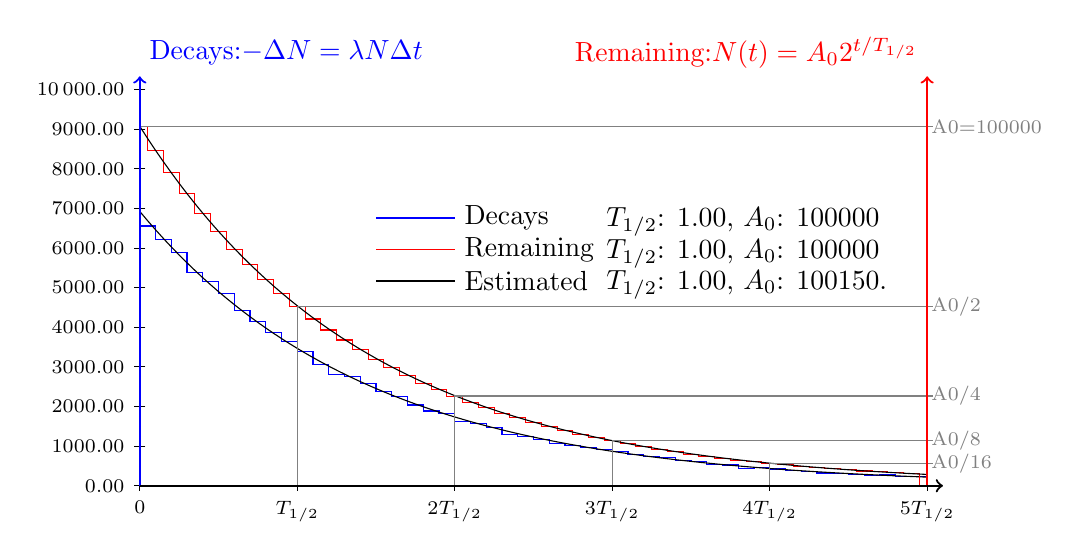
\begin{tikzpicture}[]
\begin{scope}[]
\clip (0.0,0.0) rectangle (10.0,5.0);
\begin{scope}[shift={(0.0,0.0)}]
\pgfsetxvec{\pgfpoint{2.0cm}{0cm}}
\pgfsetyvec{\pgfpoint{0cm}{0.0005cm}}
\begin{scope}[shift={(0.0,0.0)}]
\begin{scope}[draw=blue]
\pgfpathmoveto{ \pgfpointxy {5.0} {0.0}}
\pgfpathlineto{ \pgfpointxy {5.0} {230.0}}
\pgfpathlineto{ \pgfpointxy {4.9} {230.0}}
\pgfpathlineto{ \pgfpointxy {4.9} {244.0}}
\pgfpathlineto{ \pgfpointxy {4.8} {244.0}}
\pgfpathlineto{ \pgfpointxy {4.8} {271.0}}
\pgfpathlineto{ \pgfpointxy {4.7000003} {271.0}}
\pgfpathlineto{ \pgfpointxy {4.7000003} {264.0}}
\pgfpathlineto{ \pgfpointxy {4.6} {264.0}}
\pgfpathlineto{ \pgfpointxy {4.6} {290.0}}
\pgfpathlineto{ \pgfpointxy {4.5} {290.0}}
\pgfpathlineto{ \pgfpointxy {4.5} {306.0}}
\pgfpathlineto{ \pgfpointxy {4.4} {306.0}}
\pgfpathlineto{ \pgfpointxy {4.4} {322.0}}
\pgfpathlineto{ \pgfpointxy {4.3} {322.0}}
\pgfpathlineto{ \pgfpointxy {4.3} {365.0}}
\pgfpathlineto{ \pgfpointxy {4.2000003} {365.0}}
\pgfpathlineto{ \pgfpointxy {4.2000003} {394.0}}
\pgfpathlineto{ \pgfpointxy {4.1} {394.0}}
\pgfpathlineto{ \pgfpointxy {4.1} {423.0}}
\pgfpathlineto{ \pgfpointxy {4.0} {423.0}}
\pgfpathlineto{ \pgfpointxy {4.0} {457.0}}
\pgfpathlineto{ \pgfpointxy {3.9} {457.0}}
\pgfpathlineto{ \pgfpointxy {3.9} {443.0}}
\pgfpathlineto{ \pgfpointxy {3.8} {443.0}}
\pgfpathlineto{ \pgfpointxy {3.8} {525.0}}
\pgfpathlineto{ \pgfpointxy {3.7} {525.0}}
\pgfpathlineto{ \pgfpointxy {3.7} {536.0}}
\pgfpathlineto{ \pgfpointxy {3.6000001} {536.0}}
\pgfpathlineto{ \pgfpointxy {3.6000001} {613.0}}
\pgfpathlineto{ \pgfpointxy {3.5} {613.0}}
\pgfpathlineto{ \pgfpointxy {3.5} {630.0}}
\pgfpathlineto{ \pgfpointxy {3.4} {630.0}}
\pgfpathlineto{ \pgfpointxy {3.4} {714.0}}
\pgfpathlineto{ \pgfpointxy {3.3} {714.0}}
\pgfpathlineto{ \pgfpointxy {3.3} {730.0}}
\pgfpathlineto{ \pgfpointxy {3.2} {730.0}}
\pgfpathlineto{ \pgfpointxy {3.2} {785.0}}
\pgfpathlineto{ \pgfpointxy {3.1000001} {785.0}}
\pgfpathlineto{ \pgfpointxy {3.1000001} {864.0}}
\pgfpathlineto{ \pgfpointxy {3.0} {864.0}}
\pgfpathlineto{ \pgfpointxy {3.0} {910.0}}
\pgfpathlineto{ \pgfpointxy {2.9} {910.0}}
\pgfpathlineto{ \pgfpointxy {2.9} {965.0}}
\pgfpathlineto{ \pgfpointxy {2.8} {965.0}}
\pgfpathlineto{ \pgfpointxy {2.8} {1009.0}}
\pgfpathlineto{ \pgfpointxy {2.7} {1009.0}}
\pgfpathlineto{ \pgfpointxy {2.7} {1078.0}}
\pgfpathlineto{ \pgfpointxy {2.6000001} {1078.0}}
\pgfpathlineto{ \pgfpointxy {2.6000001} {1173.0}}
\pgfpathlineto{ \pgfpointxy {2.5} {1173.0}}
\pgfpathlineto{ \pgfpointxy {2.5} {1253.0}}
\pgfpathlineto{ \pgfpointxy {2.4} {1253.0}}
\pgfpathlineto{ \pgfpointxy {2.4} {1301.0}}
\pgfpathlineto{ \pgfpointxy {2.3} {1301.0}}
\pgfpathlineto{ \pgfpointxy {2.3} {1470.0}}
\pgfpathlineto{ \pgfpointxy {2.2} {1470.0}}
\pgfpathlineto{ \pgfpointxy {2.2} {1571.0}}
\pgfpathlineto{ \pgfpointxy {2.1000001} {1571.0}}
\pgfpathlineto{ \pgfpointxy {2.1000001} {1628.0}}
\pgfpathlineto{ \pgfpointxy {2.0} {1628.0}}
\pgfpathlineto{ \pgfpointxy {2.0} {1820.0}}
\pgfpathlineto{ \pgfpointxy {1.9} {1820.0}}
\pgfpathlineto{ \pgfpointxy {1.9} {1888.0}}
\pgfpathlineto{ \pgfpointxy {1.8000001} {1888.0}}
\pgfpathlineto{ \pgfpointxy {1.8000001} {2038.0}}
\pgfpathlineto{ \pgfpointxy {1.7} {2038.0}}
\pgfpathlineto{ \pgfpointxy {1.7} {2248.0}}
\pgfpathlineto{ \pgfpointxy {1.6} {2248.0}}
\pgfpathlineto{ \pgfpointxy {1.6} {2377.0}}
\pgfpathlineto{ \pgfpointxy {1.5} {2377.0}}
\pgfpathlineto{ \pgfpointxy {1.5} {2587.0}}
\pgfpathlineto{ \pgfpointxy {1.4} {2587.0}}
\pgfpathlineto{ \pgfpointxy {1.4} {2757.0}}
\pgfpathlineto{ \pgfpointxy {1.3000001} {2757.0}}
\pgfpathlineto{ \pgfpointxy {1.3000001} {2808.0}}
\pgfpathlineto{ \pgfpointxy {1.2} {2808.0}}
\pgfpathlineto{ \pgfpointxy {1.2} {3051.0}}
\pgfpathlineto{ \pgfpointxy {1.1} {3051.0}}
\pgfpathlineto{ \pgfpointxy {1.1} {3400.0}}
\pgfpathlineto{ \pgfpointxy {1.0} {3400.0}}
\pgfpathlineto{ \pgfpointxy {1.0} {3649.0}}
\pgfpathlineto{ \pgfpointxy {0.90000004} {3649.0}}
\pgfpathlineto{ \pgfpointxy {0.90000004} {3867.0}}
\pgfpathlineto{ \pgfpointxy {0.8} {3867.0}}
\pgfpathlineto{ \pgfpointxy {0.8} {4156.0}}
\pgfpathlineto{ \pgfpointxy {0.7} {4156.0}}
\pgfpathlineto{ \pgfpointxy {0.7} {4418.0}}
\pgfpathlineto{ \pgfpointxy {0.6} {4418.0}}
\pgfpathlineto{ \pgfpointxy {0.6} {4852.0}}
\pgfpathlineto{ \pgfpointxy {0.5} {4852.0}}
\pgfpathlineto{ \pgfpointxy {0.5} {5148.0}}
\pgfpathlineto{ \pgfpointxy {0.4} {5148.0}}
\pgfpathlineto{ \pgfpointxy {0.4} {5388.0}}
\pgfpathlineto{ \pgfpointxy {0.3} {5388.0}}
\pgfpathlineto{ \pgfpointxy {0.3} {5879.0}}
\pgfpathlineto{ \pgfpointxy {0.2} {5879.0}}
\pgfpathlineto{ \pgfpointxy {0.2} {6228.0}}
\pgfpathlineto{ \pgfpointxy {0.1} {6228.0}}
\pgfpathlineto{ \pgfpointxy {0.1} {6559.0}}
\pgfpathlineto{ \pgfpointxy {0.0} {6559.0}}
\pgfpathlineto{ \pgfpointxy {0.0} {0.0}}
\pgfusepath{ stroke, }
\end{scope}
\begin{scope}[black]
\pgfpathmoveto{ \pgfpointxy {0.0} {6926.170748444656}}
\pgfpathlineto{ \pgfpointxy {0.05} {6690.763194658762}}
\pgfpathlineto{ \pgfpointxy {0.1} {6463.356702121886}}
\pgfpathlineto{ \pgfpointxy {0.15} {6243.6793297680715}}
\pgfpathlineto{ \pgfpointxy {0.2} {6031.468379298172}}
\pgfpathlineto{ \pgfpointxy {0.25} {5826.470081035544}}
\pgfpathlineto{ \pgfpointxy {0.3} {5628.439290458907}}
\pgfpathlineto{ \pgfpointxy {0.35} {5437.139195049494}}
\pgfpathlineto{ \pgfpointxy {0.4} {5252.341031101914}}
\pgfpathlineto{ \pgfpointxy {0.45} {5073.823810160078}}
\pgfpathlineto{ \pgfpointxy {0.5} {4901.374054751056}}
\pgfpathlineto{ \pgfpointxy {0.55} {4734.785543100849}}
\pgfpathlineto{ \pgfpointxy {0.6} {4573.859062526792}}
\pgfpathlineto{ \pgfpointxy {0.65} {4418.402171211678}}
\pgfpathlineto{ \pgfpointxy {0.7} {4268.228968074752}}
\pgfpathlineto{ \pgfpointxy {0.75} {4123.159870464329}}
\pgfpathlineto{ \pgfpointxy {0.8} {3983.0213994062588}}
\pgfpathlineto{ \pgfpointxy {0.85} {3847.645972151357}}
\pgfpathlineto{ \pgfpointxy {0.9} {3716.87170177379}}
\pgfpathlineto{ \pgfpointxy {0.95} {3590.5422035807132}}
\pgfpathlineto{ \pgfpointxy {1.0} {3468.506408101695}}
\pgfpathlineto{ \pgfpointxy {1.05} {3350.618380434276}}
\pgfpathlineto{ \pgfpointxy {1.1} {3236.7371457296285}}
\pgfpathlineto{ \pgfpointxy {1.15} {3126.726520609644}}
\pgfpathlineto{ \pgfpointxy {1.2} {3020.4549503138232}}
\pgfpathlineto{ \pgfpointxy {1.25} {2917.7953513812467}}
\pgfpathlineto{ \pgfpointxy {1.3} {2818.624959679489}}
\pgfpathlineto{ \pgfpointxy {1.35} {2722.825183598743}}
\pgfpathlineto{ \pgfpointxy {1.4} {2630.2814622356013}}
\pgfpathlineto{ \pgfpointxy {1.45} {2540.8831283969052}}
\pgfpathlineto{ \pgfpointxy {1.5} {2454.523276259837}}
\pgfpathlineto{ \pgfpointxy {1.55} {2371.098633529997}}
\pgfpathlineto{ \pgfpointxy {1.6} {2290.509437944584}}
\pgfpathlineto{ \pgfpointxy {1.65} {2212.6593179730085}}
\pgfpathlineto{ \pgfpointxy {1.7} {2137.4551775722593}}
\pgfpathlineto{ \pgfpointxy {1.75} {2064.80708485923}}
\pgfpathlineto{ \pgfpointxy {1.8} {1994.6281645668525}}
\pgfpathlineto{ \pgfpointxy {1.85} {1926.8344941554537}}
\pgfpathlineto{ \pgfpointxy {1.9} {1861.3450034550874}}
\pgfpathlineto{ \pgfpointxy {1.95} {1798.0813777188384}}
\pgfpathlineto{ \pgfpointxy {2.0} {1736.967963971161}}
\pgfpathlineto{ \pgfpointxy {2.05} {1677.9316805392607}}
\pgfpathlineto{ \pgfpointxy {2.1} {1620.9019296593385}}
\pgfpathlineto{ \pgfpointxy {2.15} {1565.810513053182}}
\pgfpathlineto{ \pgfpointxy {2.2} {1512.5915503741492}}
\pgfpathlineto{ \pgfpointxy {2.25} {1461.181400425023}}
\pgfpathlineto{ \pgfpointxy {2.3} {1411.5185850535217}}
\pgfpathlineto{ \pgfpointxy {2.35} {1363.5437156344567}}
\pgfpathlineto{ \pgfpointxy {2.4} {1317.1994220506301}}
\pgfpathlineto{ \pgfpointxy {2.45} {1272.430284087526}}
\pgfpathlineto{ \pgfpointxy {2.5} {1229.182765159784}}
\pgfpathlineto{ \pgfpointxy {2.55} {1187.4051482901707}}
\pgfpathlineto{ \pgfpointxy {2.6} {1147.047474264514}}
\pgfpathlineto{ \pgfpointxy {2.65} {1108.0614818886354}}
\pgfpathlineto{ \pgfpointxy {2.7} {1070.4005502758316}}
\pgfpathlineto{ \pgfpointxy {2.75} {1034.0196430959022}}
\pgfpathlineto{ \pgfpointxy {2.8} {998.8752547190447}}
\pgfpathlineto{ \pgfpointxy {2.85} {964.9253581902192}}
\pgfpathlineto{ \pgfpointxy {2.9} {932.1293549717678}}
\pgfpathlineto{ \pgfpointxy {2.95} {900.4480263941834}}
\pgfpathlineto{ \pgfpointxy {3.0} {869.8434867569833}}
\pgfpathlineto{ \pgfpointxy {3.05} {840.2791380235891}}
\pgfpathlineto{ \pgfpointxy {3.1} {811.7196260560456}}
\pgfpathlineto{ \pgfpointxy {3.15} {784.1307983372425}}
\pgfpathlineto{ \pgfpointxy {3.2} {757.4796631300716}}
\pgfpathlineto{ \pgfpointxy {3.25} {731.7343500246944}}
\pgfpathlineto{ \pgfpointxy {3.3} {706.8640718267297}}
\pgfpathlineto{ \pgfpointxy {3.35} {682.8390877407925}}
\pgfpathlineto{ \pgfpointxy {3.4} {659.6306678053544}}
\pgfpathlineto{ \pgfpointxy {3.45} {637.2110585363964}}
\pgfpathlineto{ \pgfpointxy {3.5} {615.5534497387707}}
\pgfpathlineto{ \pgfpointxy {3.55} {594.6319424455797}}
\pgfpathlineto{ \pgfpointxy {3.6} {574.4215179472371}}
\pgfpathlineto{ \pgfpointxy {3.65} {554.8980078731744}}
\pgfpathlineto{ \pgfpointxy {3.7} {536.0380652904098}}
\pgfpathlineto{ \pgfpointxy {3.75} {517.8191367844275}}
\pgfpathlineto{ \pgfpointxy {3.8} {500.21943548897235}}
\pgfpathlineto{ \pgfpointxy {3.85} {483.21791503251205}}
\pgfpathlineto{ \pgfpointxy {3.9} {466.7942443702102}}
\pgfpathlineto{ \pgfpointxy {3.95} {450.9287834713141}}
\pgfpathlineto{ \pgfpointxy {4.0} {435.60255983288187}}
\pgfpathlineto{ \pgfpointxy {4.05} {420.7972457917633}}
\pgfpathlineto{ \pgfpointxy {4.1} {406.49513660770606}}
\pgfpathlineto{ \pgfpointxy {4.15} {392.6791292913727}}
\pgfpathlineto{ \pgfpointxy {4.2} {379.33270215195887}}
\pgfpathlineto{ \pgfpointxy {4.25} {366.4398950399428}}
\pgfpathlineto{ \pgfpointxy {4.3} {353.98529026135225}}
\pgfpathlineto{ \pgfpointxy {4.35} {341.9539941407178}}
\pgfpathlineto{ \pgfpointxy {4.4} {330.3316192106658}}
\pgfpathlineto{ \pgfpointxy {4.45} {319.1042670068554}}
\pgfpathlineto{ \pgfpointxy {4.5} {308.2585114476826}}
\pgfpathlineto{ \pgfpointxy {4.55} {297.78138277887587}}
\pgfpathlineto{ \pgfpointxy {4.6} {287.6603520637874}}
\pgfpathlineto{ \pgfpointxy {4.65} {277.8833162008277}}
\pgfpathlineto{ \pgfpointxy {4.7} {268.43858345013155}}
\pgfpathlineto{ \pgfpointxy {4.75} {259.31485945214376}}
\pgfpathlineto{ \pgfpointxy {4.8} {250.50123372140794}}
\pgfpathlineto{ \pgfpointxy {4.85} {241.9871665994058}}
\pgfpathlineto{ \pgfpointxy {4.9} {233.76247665084537}}
\pgfpathlineto{ \pgfpointxy {4.95} {225.81732848832505}}
\pgfpathlineto{ \pgfpointxy {5.0} {218.14222101081447}}
\pgfusepath{ stroke, }
\end{scope}
\end{scope}
\pgfsetxvec{\pgfpoint{1cm}{0cm}}
\pgfsetyvec{\pgfpoint{0cm}{1cm}}
\end{scope}
\end{scope}
\begin{scope}[shift={(0.0,0.0)}]
\pgfsetxvec{\pgfpoint{2.0cm}{0cm}}
\pgfsetyvec{\pgfpoint{0cm}{0.0005cm}}
\begin{scope}[shift={(0.0,0.0)}]
\begin{scope}[yshift=0cm]
\draw[black] [shift={(0.0,0.0)}] (0,2pt) -- (0,-2pt) node[below]{ \scriptsize{$0$}};
\draw[black] [shift={(1.0,0.0)}] (0,2pt) -- (0,-2pt) node[below]{ \scriptsize{$T_{1/2}$}};
\draw[black] [shift={(2.0,0.0)}] (0,2pt) -- (0,-2pt) node[below]{ \scriptsize{$2T_{1/2}$}};
\draw[black] [shift={(3.0,0.0)}] (0,2pt) -- (0,-2pt) node[below]{ \scriptsize{$3T_{1/2}$}};
\draw[black] [shift={(4.0,0.0)}] (0,2pt) -- (0,-2pt) node[below]{ \scriptsize{$4T_{1/2}$}};
\draw[black] [shift={(5.0,0.0)}] (0,2pt) -- (0,-2pt) node[below]{ \scriptsize{$5T_{1/2}$}};
\end{scope}
\begin{scope}[xshift=0cm]
\draw[black] [shift={(0.0,0.0)}] (2pt,0) -- (-2pt,0) node[left]{ \scriptsize{\num[round-mode=places,round-precision=2]{0}}};
\draw[black] [shift={(0.0,1000.0)}] (2pt,0) -- (-2pt,0) node[left]{ \scriptsize{\num[round-mode=places,round-precision=2]{1000}}};
\draw[black] [shift={(0.0,2000.0)}] (2pt,0) -- (-2pt,0) node[left]{ \scriptsize{\num[round-mode=places,round-precision=2]{2000}}};
\draw[black] [shift={(0.0,3000.0)}] (2pt,0) -- (-2pt,0) node[left]{ \scriptsize{\num[round-mode=places,round-precision=2]{3000}}};
\draw[black] [shift={(0.0,4000.0)}] (2pt,0) -- (-2pt,0) node[left]{ \scriptsize{\num[round-mode=places,round-precision=2]{4000}}};
\draw[black] [shift={(0.0,5000.0)}] (2pt,0) -- (-2pt,0) node[left]{ \scriptsize{\num[round-mode=places,round-precision=2]{5000}}};
\draw[black] [shift={(0.0,6000.0)}] (2pt,0) -- (-2pt,0) node[left]{ \scriptsize{\num[round-mode=places,round-precision=2]{6000}}};
\draw[black] [shift={(0.0,7000.0)}] (2pt,0) -- (-2pt,0) node[left]{ \scriptsize{\num[round-mode=places,round-precision=2]{7000}}};
\draw[black] [shift={(0.0,8000.0)}] (2pt,0) -- (-2pt,0) node[left]{ \scriptsize{\num[round-mode=places,round-precision=2]{8000}}};
\draw[black] [shift={(0.0,9000.0)}] (2pt,0) -- (-2pt,0) node[left]{ \scriptsize{\num[round-mode=places,round-precision=2]{9000}}};
\draw[black] [shift={(0.0,10000.0)}] (2pt,0) -- (-2pt,0) node[left]{ \scriptsize{\num[round-mode=places,round-precision=2]{10000}}};
\end{scope}
\end{scope}
\pgfsetxvec{\pgfpoint{1cm}{0cm}}
\pgfsetyvec{\pgfpoint{0cm}{1cm}}
\end{scope}
\begin{scope}[]
\clip (0.0,0.0) rectangle (10.0,5.0);
\begin{scope}[shift={(0.0,0.0)}]
\pgfsetxvec{\pgfpoint{2.0cm}{0cm}}
\pgfsetyvec{\pgfpoint{0cm}{0.00005cm}}
\begin{scope}[shift={(0.0,0.0)}]
\begin{scope}[draw=red]
\pgfpathmoveto{ \pgfpointxy {4.95} {0.0}}
\pgfpathlineto{ \pgfpointxy {4.95} {3348.0}}
\pgfpathlineto{ \pgfpointxy {4.85} {3348.0}}
\pgfpathlineto{ \pgfpointxy {4.85} {3592.0}}
\pgfpathlineto{ \pgfpointxy {4.75} {3592.0}}
\pgfpathlineto{ \pgfpointxy {4.75} {3863.0}}
\pgfpathlineto{ \pgfpointxy {4.65} {3863.0}}
\pgfpathlineto{ \pgfpointxy {4.65} {4127.0}}
\pgfpathlineto{ \pgfpointxy {4.5499997} {4127.0}}
\pgfpathlineto{ \pgfpointxy {4.5499997} {4417.0}}
\pgfpathlineto{ \pgfpointxy {4.45} {4417.0}}
\pgfpathlineto{ \pgfpointxy {4.45} {4723.0}}
\pgfpathlineto{ \pgfpointxy {4.35} {4723.0}}
\pgfpathlineto{ \pgfpointxy {4.35} {5045.0}}
\pgfpathlineto{ \pgfpointxy {4.25} {5045.0}}
\pgfpathlineto{ \pgfpointxy {4.25} {5410.0}}
\pgfpathlineto{ \pgfpointxy {4.15} {5410.0}}
\pgfpathlineto{ \pgfpointxy {4.15} {5804.0}}
\pgfpathlineto{ \pgfpointxy {4.0499997} {5804.0}}
\pgfpathlineto{ \pgfpointxy {4.0499997} {6227.0}}
\pgfpathlineto{ \pgfpointxy {3.95} {6227.0}}
\pgfpathlineto{ \pgfpointxy {3.95} {6684.0}}
\pgfpathlineto{ \pgfpointxy {3.8500001} {6684.0}}
\pgfpathlineto{ \pgfpointxy {3.8500001} {7127.0}}
\pgfpathlineto{ \pgfpointxy {3.75} {7127.0}}
\pgfpathlineto{ \pgfpointxy {3.75} {7652.0}}
\pgfpathlineto{ \pgfpointxy {3.65} {7652.0}}
\pgfpathlineto{ \pgfpointxy {3.65} {8188.0}}
\pgfpathlineto{ \pgfpointxy {3.5500002} {8188.0}}
\pgfpathlineto{ \pgfpointxy {3.5500002} {8801.0}}
\pgfpathlineto{ \pgfpointxy {3.45} {8801.0}}
\pgfpathlineto{ \pgfpointxy {3.45} {9431.0}}
\pgfpathlineto{ \pgfpointxy {3.3500001} {9431.0}}
\pgfpathlineto{ \pgfpointxy {3.3500001} {10145.0}}
\pgfpathlineto{ \pgfpointxy {3.25} {10145.0}}
\pgfpathlineto{ \pgfpointxy {3.25} {10875.0}}
\pgfpathlineto{ \pgfpointxy {3.15} {10875.0}}
\pgfpathlineto{ \pgfpointxy {3.15} {11660.0}}
\pgfpathlineto{ \pgfpointxy {3.0500002} {11660.0}}
\pgfpathlineto{ \pgfpointxy {3.0500002} {12524.0}}
\pgfpathlineto{ \pgfpointxy {2.95} {12524.0}}
\pgfpathlineto{ \pgfpointxy {2.95} {13434.0}}
\pgfpathlineto{ \pgfpointxy {2.8500001} {13434.0}}
\pgfpathlineto{ \pgfpointxy {2.8500001} {14399.0}}
\pgfpathlineto{ \pgfpointxy {2.75} {14399.0}}
\pgfpathlineto{ \pgfpointxy {2.75} {15408.0}}
\pgfpathlineto{ \pgfpointxy {2.65} {15408.0}}
\pgfpathlineto{ \pgfpointxy {2.65} {16486.0}}
\pgfpathlineto{ \pgfpointxy {2.5500002} {16486.0}}
\pgfpathlineto{ \pgfpointxy {2.5500002} {17659.0}}
\pgfpathlineto{ \pgfpointxy {2.45} {17659.0}}
\pgfpathlineto{ \pgfpointxy {2.45} {18912.0}}
\pgfpathlineto{ \pgfpointxy {2.3500001} {18912.0}}
\pgfpathlineto{ \pgfpointxy {2.3500001} {20213.0}}
\pgfpathlineto{ \pgfpointxy {2.25} {20213.0}}
\pgfpathlineto{ \pgfpointxy {2.25} {21683.0}}
\pgfpathlineto{ \pgfpointxy {2.15} {21683.0}}
\pgfpathlineto{ \pgfpointxy {2.15} {23254.0}}
\pgfpathlineto{ \pgfpointxy {2.0500002} {23254.0}}
\pgfpathlineto{ \pgfpointxy {2.0500002} {24882.0}}
\pgfpathlineto{ \pgfpointxy {1.95} {24882.0}}
\pgfpathlineto{ \pgfpointxy {1.95} {26702.0}}
\pgfpathlineto{ \pgfpointxy {1.85} {26702.0}}
\pgfpathlineto{ \pgfpointxy {1.85} {28590.0}}
\pgfpathlineto{ \pgfpointxy {1.7500001} {28590.0}}
\pgfpathlineto{ \pgfpointxy {1.7500001} {30628.0}}
\pgfpathlineto{ \pgfpointxy {1.6500001} {30628.0}}
\pgfpathlineto{ \pgfpointxy {1.6500001} {32876.0}}
\pgfpathlineto{ \pgfpointxy {1.5500001} {32876.0}}
\pgfpathlineto{ \pgfpointxy {1.5500001} {35253.0}}
\pgfpathlineto{ \pgfpointxy {1.45} {35253.0}}
\pgfpathlineto{ \pgfpointxy {1.45} {37840.0}}
\pgfpathlineto{ \pgfpointxy {1.35} {37840.0}}
\pgfpathlineto{ \pgfpointxy {1.35} {40597.0}}
\pgfpathlineto{ \pgfpointxy {1.2500001} {40597.0}}
\pgfpathlineto{ \pgfpointxy {1.2500001} {43405.0}}
\pgfpathlineto{ \pgfpointxy {1.1500001} {43405.0}}
\pgfpathlineto{ \pgfpointxy {1.1500001} {46456.0}}
\pgfpathlineto{ \pgfpointxy {1.0500001} {46456.0}}
\pgfpathlineto{ \pgfpointxy {1.0500001} {49856.0}}
\pgfpathlineto{ \pgfpointxy {0.95} {49856.0}}
\pgfpathlineto{ \pgfpointxy {0.95} {53505.0}}
\pgfpathlineto{ \pgfpointxy {0.85} {53505.0}}
\pgfpathlineto{ \pgfpointxy {0.85} {57372.0}}
\pgfpathlineto{ \pgfpointxy {0.75} {57372.0}}
\pgfpathlineto{ \pgfpointxy {0.75} {61528.0}}
\pgfpathlineto{ \pgfpointxy {0.65} {61528.0}}
\pgfpathlineto{ \pgfpointxy {0.65} {65946.0}}
\pgfpathlineto{ \pgfpointxy {0.55} {65946.0}}
\pgfpathlineto{ \pgfpointxy {0.55} {70798.0}}
\pgfpathlineto{ \pgfpointxy {0.45} {70798.0}}
\pgfpathlineto{ \pgfpointxy {0.45} {75946.0}}
\pgfpathlineto{ \pgfpointxy {0.35} {75946.0}}
\pgfpathlineto{ \pgfpointxy {0.35} {81334.0}}
\pgfpathlineto{ \pgfpointxy {0.25} {81334.0}}
\pgfpathlineto{ \pgfpointxy {0.25} {87213.0}}
\pgfpathlineto{ \pgfpointxy {0.15} {87213.0}}
\pgfpathlineto{ \pgfpointxy {0.15} {93441.0}}
\pgfpathlineto{ \pgfpointxy {0.05} {93441.0}}
\pgfpathlineto{ \pgfpointxy {0.05} {100000.0}}
\pgfpathlineto{ \pgfpointxy {-0.05} {100000.0}}
\pgfpathlineto{ \pgfpointxy {-0.05} {0.0}}
\pgfusepath{ stroke, }
\end{scope}
\begin{scope}[black]
\pgfpathmoveto{ \pgfpointxy {0.0} {100149.51712276821}}
\pgfpathlineto{ \pgfpointxy {0.05} {96745.62286503517}}
\pgfpathlineto{ \pgfpointxy {0.1} {93457.42058915786}}
\pgfpathlineto{ \pgfpointxy {0.15} {90280.978141652}}
\pgfpathlineto{ \pgfpointxy {0.2} {87212.4970155555}}
\pgfpathlineto{ \pgfpointxy {0.25} {84248.3078080339}}
\pgfpathlineto{ \pgfpointxy {0.3} {81384.86583237312}}
\pgfpathlineto{ \pgfpointxy {0.35} {78618.74687911248}}
\pgfpathlineto{ \pgfpointxy {0.4} {75946.64312124884}}
\pgfpathlineto{ \pgfpointxy {0.45} {73365.35915861506}}
\pgfpathlineto{ \pgfpointxy {0.5} {70871.80819670274}}
\pgfpathlineto{ \pgfpointxy {0.55} {68463.00835535962}}
\pgfpathlineto{ \pgfpointxy {0.6} {66136.0791029473}}
\pgfpathlineto{ \pgfpointxy {0.65} {63888.23781169537}}
\pgfpathlineto{ \pgfpointxy {0.7} {61716.796430132556}}
\pgfpathlineto{ \pgfpointxy {0.75} {59619.15826861566}}
\pgfpathlineto{ \pgfpointxy {0.8} {57592.814894112445}}
\pgfpathlineto{ \pgfpointxy {0.85} {55635.34313052484}}
\pgfpathlineto{ \pgfpointxy {0.9} {53744.40216096576}}
\pgfpathlineto{ \pgfpointxy {0.95} {51917.730728523915}}
\pgfpathlineto{ \pgfpointxy {1.0} {50153.14443216944}}
\pgfpathlineto{ \pgfpointxy {1.05} {48448.53311456674}}
\pgfpathlineto{ \pgfpointxy {1.1} {46801.858338670376}}
\pgfpathlineto{ \pgfpointxy {1.15} {45211.15095008709}}
\pgfpathlineto{ \pgfpointxy {1.2} {43674.50872228831}}
\pgfpathlineto{ \pgfpointxy {1.25} {42190.09408185753}}
\pgfpathlineto{ \pgfpointxy {1.3} {40756.13191105239}}
\pgfpathlineto{ \pgfpointxy {1.35} {39370.90742505332}}
\pgfpathlineto{ \pgfpointxy {1.4} {38032.764121360735}}
\pgfpathlineto{ \pgfpointxy {1.45} {36740.10179888826}}
\pgfpathlineto{ \pgfpointxy {1.5} {35491.37464438326}}
\pgfpathlineto{ \pgfpointxy {1.55} {34285.08938388645}}
\pgfpathlineto{ \pgfpointxy {1.6} {33119.80349701976}}
\pgfpathlineto{ \pgfpointxy {1.65} {31994.123491967377}}
\pgfpathlineto{ \pgfpointxy {1.7} {30906.703239086783}}
\pgfpathlineto{ \pgfpointxy {1.75} {29856.242361157398}}
\pgfpathlineto{ \pgfpointxy {1.8} {28841.484678341516}}
\pgfpathlineto{ \pgfpointxy {1.85} {27861.216705998162}}
\pgfpathlineto{ \pgfpointxy {1.9} {26914.266203553427}}
\pgfpathlineto{ \pgfpointxy {1.95} {25999.500772691987}}
\pgfpathlineto{ \pgfpointxy {2.0} {25115.826503193468}}
\pgfpathlineto{ \pgfpointxy {2.05} {24262.186664794248}}
\pgfpathlineto{ \pgfpointxy {2.1} {23437.560443510498}}
\pgfpathlineto{ \pgfpointxy {2.15} {22640.961720911168}}
\pgfpathlineto{ \pgfpointxy {2.2} {21871.437894881234}}
\pgfpathlineto{ \pgfpointxy {2.25} {21128.068740464954}}
\pgfpathlineto{ \pgfpointxy {2.3} {20409.965309426967}}
\pgfpathlineto{ \pgfpointxy {2.35} {19716.268867215207}}
\pgfpathlineto{ \pgfpointxy {2.4} {19046.14986605453}}
\pgfpathlineto{ \pgfpointxy {2.45} {18398.806952942792}}
\pgfpathlineto{ \pgfpointxy {2.5} {17773.466011363525}}
\pgfpathlineto{ \pgfpointxy {2.55} {17169.379235568784}}
\pgfpathlineto{ \pgfpointxy {2.6} {16585.824236325483}}
\pgfpathlineto{ \pgfpointxy {2.65} {16022.103177055762}}
\pgfpathlineto{ \pgfpointxy {2.7} {15477.541939338244}}
\pgfpathlineto{ \pgfpointxy {2.75} {14951.489316772395}}
\pgfpathlineto{ \pgfpointxy {2.8} {14443.316236241903}}
\pgfpathlineto{ \pgfpointxy {2.85} {13952.415005645857}}
\pgfpathlineto{ \pgfpointxy {2.9} {13478.198587198156}}
\pgfpathlineto{ \pgfpointxy {2.95} {13020.099895426034}}
\pgfpathlineto{ \pgfpointxy {3.0} {12577.571119028411}}
\pgfpathlineto{ \pgfpointxy {3.05} {12150.08306578291}}
\pgfpathlineto{ \pgfpointxy {3.1} {11737.124529718276}}
\pgfpathlineto{ \pgfpointxy {3.15} {11338.20167979549}}
\pgfpathlineto{ \pgfpointxy {3.2} {10952.83746936635}}
\pgfpathlineto{ \pgfpointxy {3.25} {10580.571065703547}}
\pgfpathlineto{ \pgfpointxy {3.3} {10220.957298919873}}
\pgfpathlineto{ \pgfpointxy {3.35} {9873.566129617686}}
\pgfpathlineto{ \pgfpointxy {3.4} {9537.982134631926}}
\pgfpathlineto{ \pgfpointxy {3.45} {9213.804010251803}}
\pgfpathlineto{ \pgfpointxy {3.5} {8900.644092327007}}
\pgfpathlineto{ \pgfpointxy {3.55} {8598.12789268465}}
\pgfpathlineto{ \pgfpointxy {3.6} {8305.89365130247}}
\pgfpathlineto{ \pgfpointxy {3.65} {8023.591903702907}}
\pgfpathlineto{ \pgfpointxy {3.7} {7750.885063050566}}
\pgfpathlineto{ \pgfpointxy {3.75} {7487.447016453448}}
\pgfpathlineto{ \pgfpointxy {3.8} {7232.9627349851335}}
\pgfpathlineto{ \pgfpointxy {3.85} {6987.12789696158}}
\pgfpathlineto{ \pgfpointxy {3.9} {6749.648524022027}}
\pgfpathlineto{ \pgfpointxy {3.95} {6520.240629578851}}
\pgfpathlineto{ \pgfpointxy {4.0} {6298.62987921593}}
\pgfpathlineto{ \pgfpointxy {4.05} {6084.551262629423}}
\pgfpathlineto{ \pgfpointxy {4.1} {5877.748776718706}}
\pgfpathlineto{ \pgfpointxy {4.15} {5677.975119448398}}
\pgfpathlineto{ \pgfpointxy {4.2} {5484.991394115514}}
\pgfpathlineto{ \pgfpointxy {4.25} {5298.566823667932}}
\pgfpathlineto{ \pgfpointxy {4.3} {5118.4784747327185}}
\pgfpathlineto{ \pgfpointxy {4.35} {4944.510991024184}}
\pgfpathlineto{ \pgfpointxy {4.4} {4776.456335812881}}
\pgfpathlineto{ \pgfpointxy {4.45} {4614.113543147633}}
\pgfpathlineto{ \pgfpointxy {4.5} {4457.288477533037}}
\pgfpathlineto{ \pgfpointxy {4.55} {4305.793601775066}}
\pgfpathlineto{ \pgfpointxy {4.6} {4159.447752717211}}
\pgfpathlineto{ \pgfpointxy {4.65} {4018.0759245988706}}
\pgfpathlineto{ \pgfpointxy {4.7} {3881.509059777031}}
\pgfpathlineto{ \pgfpointxy {4.75} {3749.5838465609004}}
\pgfpathlineto{ \pgfpointxy {4.8} {3622.142523917763}}
\pgfpathlineto{ \pgfpointxy {4.85} {3499.032692816526}}
\pgfpathlineto{ \pgfpointxy {4.9} {3380.1071339833443}}
\pgfpathlineto{ \pgfpointxy {4.95} {3265.2236318513847}}
\pgfpathlineto{ \pgfpointxy {5.0} {3154.2448044941984}}
\pgfusepath{ stroke, }
\end{scope}
\end{scope}
\pgfsetxvec{\pgfpoint{1cm}{0cm}}
\pgfsetyvec{\pgfpoint{0cm}{1cm}}
\end{scope}
\end{scope}
\begin{scope}[shift={(0.0,0.0)}]
\pgfsetxvec{\pgfpoint{2.0cm}{0cm}}
\pgfsetyvec{\pgfpoint{0cm}{0.00005cm}}
\begin{scope}[shift={(0.0,0.0)}]
\begin{scope}[gray]
\pgfpathmoveto{ \pgfpointxy {0.0} {0.0}}
\pgfpathlineto{ \pgfpointxy {0.0} {100000.0}}
\pgfpathlineto{ \pgfpointxy {5.0} {100000.0}}
\pgfusepath{ stroke, }
\end{scope}
\begin{scope}[gray]
\pgfpathmoveto{ \pgfpointxy {1.0} {0.0}}
\pgfpathlineto{ \pgfpointxy {1.0} {50000.0}}
\pgfpathlineto{ \pgfpointxy {5.0} {50000.0}}
\pgfusepath{ stroke, }
\end{scope}
\begin{scope}[gray]
\pgfpathmoveto{ \pgfpointxy {2.0} {0.0}}
\pgfpathlineto{ \pgfpointxy {2.0} {25000.0}}
\pgfpathlineto{ \pgfpointxy {5.0} {25000.0}}
\pgfusepath{ stroke, }
\end{scope}
\begin{scope}[gray]
\pgfpathmoveto{ \pgfpointxy {3.0} {0.0}}
\pgfpathlineto{ \pgfpointxy {3.0} {12500.0}}
\pgfpathlineto{ \pgfpointxy {5.0} {12500.0}}
\pgfusepath{ stroke, }
\end{scope}
\begin{scope}[gray]
\pgfpathmoveto{ \pgfpointxy {4.0} {0.0}}
\pgfpathlineto{ \pgfpointxy {4.0} {6250.0}}
\pgfpathlineto{ \pgfpointxy {5.0} {6250.0}}
\pgfusepath{ stroke, }
\end{scope}
\begin{scope}[xshift=10cm]
\draw[gray] [shift={(0.0,100000.0)}] (2pt,0) -- (-2pt,0) node[right]{ \scriptsize{A0=100000}};
\draw[gray] [shift={(0.0,50000.0)}] (2pt,0) -- (-2pt,0) node[right]{ \scriptsize{A0/2}};
\draw[gray] [shift={(0.0,25000.0)}] (2pt,0) -- (-2pt,0) node[right]{ \scriptsize{A0/4}};
\draw[gray] [shift={(0.0,12500.0)}] (2pt,0) -- (-2pt,0) node[right]{ \scriptsize{A0/8}};
\draw[gray] [shift={(0.0,6250.0)}] (2pt,0) -- (-2pt,0) node[right]{ \scriptsize{A0/16}};
\end{scope}
\end{scope}
\pgfsetxvec{\pgfpoint{1cm}{0cm}}
\pgfsetyvec{\pgfpoint{0cm}{1cm}}
\end{scope}
\node[right,blue] at (0.0,5.5) {Decays:$-\Delta N = \lambda N \Delta t$};
\node[left,red] at (10.0,5.5) {Remaining:$N(t) = A_0 2^{t/T_{1/2}}$};
\draw[blue,thick,->] (0.0,0.0) -- (0.0,5.2);
\draw[red,thick,->] (10.0,0.0) -- (10.0,5.2);
\draw[black,thick,->] (0.0,0.0) -- (10.2,0.0);
\draw[blue] (3.0,3.4) -- (4.0,3.4);
\node[right,] at (4.0,3.4) {Decays};
\node[right] at (5.8,3.35) {$T_{1/2}$: 1.00, $A_0$: 100000};
\draw[red] (3.0,3.0) -- (4.0,3.0);
\node[right,] at (4.0,3.0) {Remaining};
\node[right] at (5.8,2.95) {$T_{1/2}$: 1.00, $A_0$: 100000};
\draw[black] (3.0,2.6) -- (4.0,2.6);
\node[right,] at (4.0,2.6) {Estimated};
\node[right] at (5.8,2.55) {$T_{1/2}$:  1.00, $A_0$: 100150.};
\end{tikzpicture}
%%% Local Variables: 
%%% mode: latex 
%%% TeX-master: "master" 
%%% End:


  \caption{Graph of radioactive decay.}
\end{figure}

\begin{figure}[H]
  \centering
  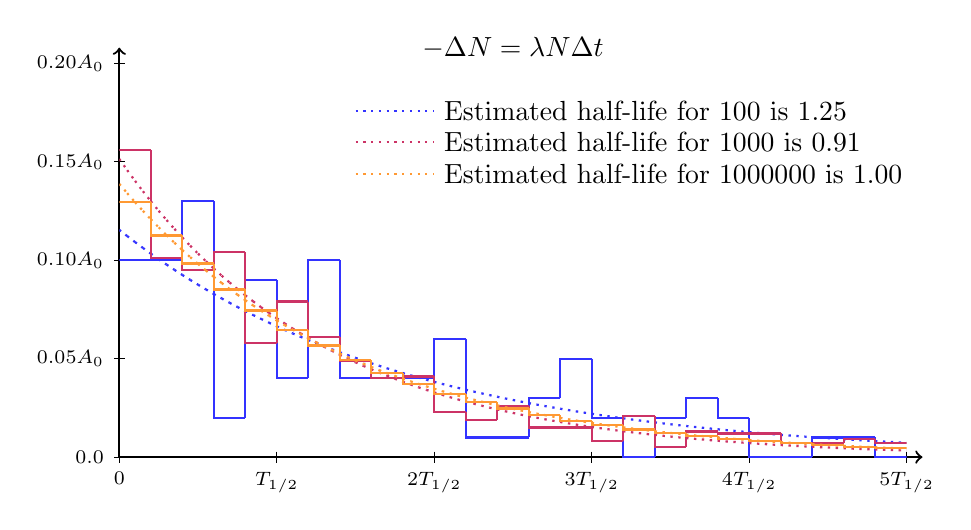
\begin{tikzpicture}
\node[] at (5.0,5.2) {$-\Delta N = \lambda N \Delta t$};
\draw[thick,->] (0.0,0.0) -- (0.0,5.2);
\draw[thick,->] (0.0,0.0) -- (10.2,0.0);
\draw (0,0cm + 2pt) -- (0, 0cm-2pt) node[below] {\scriptsize $0$};
\draw (2,0cm + 2pt) -- (2, 0cm-2pt) node[below] {\scriptsize $T_{1/2}$};
\draw (4,0cm + 2pt) -- (4, 0cm-2pt) node[below] {\scriptsize $2T_{1/2}$};
\draw (6,0cm + 2pt) -- (6, 0cm-2pt) node[below] {\scriptsize $3T_{1/2}$};
\draw (8,0cm + 2pt) -- (8, 0cm-2pt) node[below] {\scriptsize $4T_{1/2}$};
\draw (10,0cm + 2pt) -- (10, 0cm-2pt) node[below] {\scriptsize $5T_{1/2}$};
\draw (0cm+2pt,0.    ) -- (0cm-2pt,0.    ) node[left] {\scriptsize $0.0$};
\draw (0cm+2pt,1.25    ) -- (0cm-2pt,1.25    ) node[left] {\scriptsize $0.05 A_0$};
\draw (0cm+2pt,2.5    ) -- (0cm-2pt,2.5    ) node[left] {\scriptsize $0.10 A_0$};
\draw (0cm+2pt,3.750000093132256    ) -- (0cm-2pt,3.750000093132256    ) node[left] {\scriptsize $0.15 A_0$};
\draw (0cm+2pt,5.    ) -- (0cm-2pt,5.    ) node[left] {\scriptsize $0.20 A_0$};
\begin{scope}[]
\clip (0,0) rectangle (10,5);
\draw[dotted,blue!80,thick] (3.0,4.4) -- (4.0,4.4);
\node[right,] at (4.0,4.4) {Estimated half-life for 100 is  1.25};
\begin{scope}[blue!80,thick]
\draw[] (0.0,2.4999999627470975) -- (0.4,2.4999999627470975);
\draw (0.4,2.4999999627470975) -- (0.4,2.4999999627470975) -- (0.8,2.4999999627470975);
\draw (0.8,2.4999999627470975) -- (0.8,3.249999951571227) -- (1.2,3.249999951571227);
\draw (1.2,3.249999951571227) -- (1.2,0.4999999925494195) -- (1.6,0.4999999925494195);
\draw (1.6,0.4999999925494195) -- (1.6,2.2499999664723878) -- (2.0,2.2499999664723878);
\draw (2.0,2.2499999664723878) -- (2.0,0.999999985098839) -- (2.4,0.999999985098839);
\draw (2.4,0.999999985098839) -- (2.4,2.4999999627470975) -- (2.8,2.4999999627470975);
\draw (2.8,2.4999999627470975) -- (2.8,0.999999985098839) -- (3.2,0.999999985098839);
\draw (3.2,0.999999985098839) -- (3.2,0.999999985098839) -- (3.6000001,0.999999985098839);
\draw (3.6000001,0.999999985098839) -- (3.6000001,0.999999985098839) -- (4.0,0.999999985098839);
\draw (4.0,0.999999985098839) -- (4.0,1.4999999776482584) -- (4.4,1.4999999776482584);
\draw (4.4,1.4999999776482584) -- (4.4,0.24999999627470976) -- (4.8,0.24999999627470976);
\draw (4.8,0.24999999627470976) -- (4.8,0.24999999627470976) -- (5.2000003,0.24999999627470976);
\draw (5.2000003,0.24999999627470976) -- (5.2000003,0.7499999888241292) -- (5.6,0.7499999888241292);
\draw (5.6,0.7499999888241292) -- (5.6,1.2499999813735487) -- (6.0,1.2499999813735487);
\draw (6.0,1.2499999813735487) -- (6.0,0.4999999925494195) -- (6.4,0.4999999925494195);
\draw (6.4,0.4999999925494195) -- (6.4,0.0) -- (6.8,0.0);
\draw (6.8,0.0) -- (6.8,0.4999999925494195) -- (7.2000003,0.4999999925494195);
\draw (7.2000003,0.4999999925494195) -- (7.2000003,0.7499999888241292) -- (7.6,0.7499999888241292);
\draw (7.6,0.7499999888241292) -- (7.6,0.4999999925494195) -- (8.0,0.4999999925494195);
\draw (8.0,0.4999999925494195) -- (8.0,0.0) -- (8.400001,0.0);
\draw (8.400001,0.0) -- (8.400001,0.0) -- (8.8,0.0);
\draw (8.8,0.0) -- (8.8,0.24999999627470976) -- (9.2,0.24999999627470976);
\draw (9.2,0.24999999627470976) -- (9.2,0.24999999627470976) -- (9.6,0.24999999627470976);
\draw (9.6,0.24999999627470976) -- (9.6,0.0) -- (10.0,0.0);
\end{scope}
\begin{scope}[dotted,blue!80,thick]
\draw[] (0.0,2.8859633993276717) -- (0.1,2.8073169041835);
\draw[] (0.1,2.8073169041835) -- (0.2,2.7308136348334964);
\draw[] (0.2,2.7308136348334964) -- (0.3,2.656395185409778);
\draw[] (0.3,2.656395185409778) -- (0.4,2.584004741685162);
\draw[] (0.4,2.584004741685162) -- (0.5,2.5135870376987564);
\draw[] (0.5,2.5135870376987564) -- (0.6,2.4450883135635575);
\draw[] (0.6,2.4450883135635575) -- (0.7,2.378456274423857);
\draw[] (0.7,2.378456274423857) -- (0.8,2.3136400505311085);
\draw[] (0.8,2.3136400505311085) -- (0.9,2.2505901584077894);
\draw[] (0.9,2.2505901584077894) -- (1.0,2.1892584630695975);
\draw[] (1.0,2.1892584630695975) -- (1.1,2.1295981412771416);
\draw[] (1.1,2.1295981412771416) -- (1.2,2.071563645789081);
\draw[] (1.2,2.071563645789081) -- (1.3,2.015110670589414);
\draw[] (1.3,2.015110670589414) -- (1.4,1.9601961170623672);
\draw[] (1.4,1.9601961170623672) -- (1.5,1.9067780610890712);
\draw[] (1.5,1.9067780610890712) -- (1.6,1.8548157210408953);
\draw[] (1.6,1.8548157210408953) -- (1.7,1.8042694266450072);
\draw[] (1.7,1.8042694266450072) -- (1.8,1.7551005886983888);
\draw[] (1.8,1.7551005886983888) -- (1.9,1.7072716696071915);
\draw[] (1.9,1.7072716696071915) -- (2.0,1.6607461547289282);
\draw[] (2.0,1.6607461547289282) -- (2.1,1.6154885244956352);
\draw[] (2.1,1.6154885244956352) -- (2.2,1.5714642272967136);
\draw[] (2.2,1.5714642272967136) -- (2.3,1.5286396531007547);
\draw[] (2.3,1.5286396531007547) -- (2.4,1.4869821077962013);
\draw[] (2.4,1.4869821077962013) -- (2.5,1.4464597882312658);
\draw[] (2.5,1.4464597882312658) -- (2.6,1.4070417579340446);
\draw[] (2.6,1.4070417579340446) -- (2.7,1.3686979234942918);
\draw[] (2.7,1.3686979234942918) -- (2.8,1.3313990115888228);
\draw[] (2.8,1.3313990115888228) -- (2.9,1.2951165466330066);
\draw[] (2.9,1.2951165466330066) -- (3.0,1.2598228290412874);
\draw[] (3.0,1.2598228290412874) -- (3.1,1.2254909140801364);
\draw[] (3.1,1.2254909140801364) -- (3.2,1.1920945912972893);
\draw[] (3.2,1.1920945912972893) -- (3.3,1.1596083645115665);
\draw[] (3.3,1.1596083645115665) -- (3.4,1.1280074323479965);
\draw[] (3.4,1.1280074323479965) -- (3.5,1.0972676693033876);
\draw[] (3.5,1.0972676693033876) -- (3.6,1.0673656073278863);
\draw[] (3.6,1.0673656073278863) -- (3.7,1.0382784179084625);
\draw[] (3.7,1.0382784179084625) -- (3.8,1.0099838946406487);
\draw[] (3.8,1.0099838946406487) -- (3.9,0.9824604362752197);
\draw[] (3.9,0.9824604362752197) -- (4.0,0.9556870302268757);
\draw[] (4.0,0.9556870302268757) -- (4.1,0.9296432365323349);
\draw[] (4.1,0.9296432365323349) -- (4.2,0.9043091722455927);
\draw[] (4.2,0.9043091722455927) -- (4.3,0.8796654962584298);
\draw[] (4.3,0.8796654962584298) -- (4.4,0.8556933945345822);
\draw[] (4.4,0.8556933945345822) -- (4.5,0.8323745657463028);
\draw[] (4.5,0.8323745657463028) -- (4.6,0.809691207302343);
\draw[] (4.6,0.809691207302343) -- (4.7,0.7876260017566948);
\draw[] (4.7,0.7876260017566948) -- (4.8,0.7661621035877121);
\draw[] (4.8,0.7661621035877121) -- (4.9,0.7452831263375167);
\draw[] (4.9,0.7452831263375167) -- (5.0,0.7249731301018779);
\draw[] (5.0,0.7249731301018779) -- (5.1,0.7052166093610068);
\draw[] (5.1,0.7052166093610068) -- (5.2,0.6859984811419794);
\draw[] (5.2,0.6859984811419794) -- (5.3,0.6673040735037501);
\draw[] (5.3,0.6673040735037501) -- (5.4,0.6491191143359639);
\draw[] (5.4,0.6491191143359639) -- (5.5,0.6314297204630186);
\draw[] (5.5,0.6314297204630186) -- (5.6,0.6142223870450518);
\draw[] (5.6,0.6142223870450518) -- (5.7,0.5974839772677711);
\draw[] (5.7,0.5974839772677711) -- (5.8,0.581201712313248);
\draw[] (5.8,0.581201712313248) -- (5.9,0.5653631616040197);
\draw[] (5.9,0.5653631616040197) -- (6.0,0.5499562333130572);
\draw[] (6.0,0.5499562333130572) -- (6.1,0.5349691651323455);
\draw[] (6.1,0.5349691651323455) -- (6.2,0.5203905152930358);
\draw[] (6.2,0.5203905152930358) -- (6.3,0.5062091538303086);
\draw[] (6.3,0.5062091538303086) -- (6.4,0.49241425408628375);
\draw[] (6.4,0.49241425408628375) -- (6.5,0.478995284444486);
\draw[] (6.5,0.478995284444486) -- (6.6,0.4659420002895586);
\draw[] (6.6,0.4659420002895586) -- (6.7,0.45324443618608623);
\draw[] (6.7,0.45324443618608623) -- (6.8,0.4408928982705549);
\draw[] (6.8,0.4408928982705549) -- (6.9,0.4288779568506418);
\draw[] (6.9,0.4288779568506418) -- (7.0,0.4171904392061859);
\draw[] (7.0,0.4171904392061859) -- (7.1,0.40582142258633985);
\draw[] (7.1,0.40582142258633985) -- (7.2,0.3947622273975606);
\draw[] (7.2,0.3947622273975606) -- (7.3,0.3840044105772374);
\draw[] (7.3,0.3840044105772374) -- (7.4,0.3735397591478954);
\draw[] (7.4,0.3735397591478954) -- (7.5,0.3633602839470582);
\draw[] (7.5,0.3633602839470582) -- (7.6,0.3534582135279793);
\draw[] (7.6,0.3534582135279793) -- (7.7,0.34382598822658716);
\draw[] (7.7,0.34382598822658716) -- (7.8,0.3344562543901145);
\draw[] (7.8,0.3344562543901145) -- (7.9,0.32534185876300503);
\draw[] (7.9,0.32534185876300503) -- (8.0,0.3164758430258128);
\draw[] (8.0,0.3164758430258128) -- (8.1,0.30785143848292235);
\draw[] (8.1,0.30785143848292235) -- (8.2,0.2994620608950383);
\draw[] (8.2,0.2994620608950383) -- (8.3,0.2913013054524945);
\draw[] (8.3,0.2913013054524945) -- (8.4,0.2833629418855492);
\draw[] (8.4,0.2833629418855492) -- (8.5,0.27564090970792987);
\draw[] (8.5,0.27564090970792987) -- (8.6,0.2681293135899994);
\draw[] (8.6,0.2681293135899994) -- (8.7,0.2608224188580085);
\draw[] (8.7,0.2608224188580085) -- (8.8,0.25371464711600145);
\draw[] (8.8,0.25371464711600145) -- (8.9,0.24680057198702998);
\draw[] (8.9,0.24680057198702998) -- (9.0,0.24007491497042385);
\draw[] (9.0,0.24007491497042385) -- (9.1,0.23353254141195898);
\draw[] (9.1,0.23353254141195898) -- (9.2,0.22716845658384213);
\draw[] (9.2,0.22716845658384213) -- (9.3,0.22097780187152244);
\draw[] (9.3,0.22097780187152244) -- (9.4,0.2149558510644169);
\draw[] (9.4,0.2149558510644169) -- (9.5,0.20909800674771928);
\draw[] (9.5,0.20909800674771928) -- (9.6,0.20339979679253714);
\draw[] (9.6,0.20339979679253714) -- (9.7,0.197856870941677);
\draw[] (9.7,0.197856870941677) -- (9.8,0.19246499748847212);
\draw[] (9.8,0.19246499748847212) -- (9.9,0.18722006004611705);
\draw[] (9.9,0.18722006004611705) -- (10.0,0.18211805440504114);
\end{scope}
\draw[dotted,purple!80,thick] (3.0,4.0) -- (4.0,4.0);
\node[right,] at (4.0,4.0) {Estimated half-life for 1000 is  0.91};
\begin{scope}[purple!80,thick]
\draw[] (0.0,3.899999941885472) -- (0.4,3.899999941885472);
\draw (0.4,3.899999941885472) -- (0.4,2.5249999623745687) -- (0.8,2.5249999623745687);
\draw (0.8,2.5249999623745687) -- (0.8,2.3749999646097426) -- (1.2,2.3749999646097426);
\draw (1.2,2.3749999646097426) -- (1.2,2.599999961256981) -- (1.6,2.599999961256981);
\draw (1.6,2.599999961256981) -- (1.6,1.4499999783933166) -- (2.0,1.4499999783933166);
\draw (2.0,1.4499999783933166) -- (2.0,1.974999970570207) -- (2.4,1.974999970570207);
\draw (2.4,1.974999970570207) -- (2.4,1.5249999772757294) -- (2.8,1.5249999772757294);
\draw (2.8,1.5249999772757294) -- (2.8,1.2249999817460777) -- (3.2,1.2249999817460777);
\draw (3.2,1.2249999817460777) -- (3.2,0.999999985098839) -- (3.6000001,0.999999985098839);
\draw (3.6000001,0.999999985098839) -- (3.6000001,1.02499998472631) -- (4.0,1.02499998472631);
\draw (4.0,1.02499998472631) -- (4.0,0.5749999914318324) -- (4.4,0.5749999914318324);
\draw (4.4,0.5749999914318324) -- (4.4,0.4749999929219485) -- (4.8,0.4749999929219485);
\draw (4.8,0.4749999929219485) -- (4.8,0.6499999903142453) -- (5.2000003,0.6499999903142453);
\draw (5.2000003,0.6499999903142453) -- (5.2000003,0.3749999944120646) -- (5.6,0.3749999944120646);
\draw (5.6,0.3749999944120646) -- (5.6,0.3749999944120646) -- (6.0,0.3749999944120646);
\draw (6.0,0.3749999944120646) -- (6.0,0.1999999970197678) -- (6.4,0.1999999970197678);
\draw (6.4,0.1999999970197678) -- (6.4,0.5249999921768905) -- (6.8,0.5249999921768905);
\draw (6.8,0.5249999921768905) -- (6.8,0.12499999813735488) -- (7.2000003,0.12499999813735488);
\draw (7.2000003,0.12499999813735488) -- (7.2000003,0.32499999515712263) -- (7.6,0.32499999515712263);
\draw (7.6,0.32499999515712263) -- (7.6,0.29999999552965173) -- (8.0,0.29999999552965173);
\draw (8.0,0.29999999552965173) -- (8.0,0.29999999552965173) -- (8.400001,0.29999999552965173);
\draw (8.400001,0.29999999552965173) -- (8.400001,0.17499999739229682) -- (8.8,0.17499999739229682);
\draw (8.8,0.17499999739229682) -- (8.8,0.17499999739229682) -- (9.2,0.17499999739229682);
\draw (9.2,0.17499999739229682) -- (9.2,0.22499999664723877) -- (9.6,0.22499999664723877);
\draw (9.6,0.22499999664723877) -- (9.6,0.17499999739229682) -- (10.0,0.17499999739229682);
\end{scope}
\begin{scope}[dotted,purple!80,thick]
\draw[] (0.0,3.7861231998413127) -- (0.1,3.644226858191287);
\draw[] (0.1,3.644226858191287) -- (0.2,3.5076485082469993);
\draw[] (0.2,3.5076485082469993) -- (0.3,3.3761888422923154);
\draw[] (0.3,3.3761888422923154) -- (0.4,3.2496560222665445);
\draw[] (0.4,3.2496560222665445) -- (0.5,3.1278653998166663);
\draw[] (0.5,3.1278653998166663) -- (0.6,3.0106392468414325);
\draw[] (0.6,3.0106392468414325) -- (0.7,2.897806496134141);
\draw[] (0.7,2.897806496134141) -- (0.8,2.789202491745602);
\draw[] (0.8,2.789202491745602) -- (0.9,2.684668748703002);
\draw[] (0.9,2.684668748703002) -- (1.0,2.584052721734024);
\draw[] (1.0,2.584052721734024) -- (1.1,2.487207582658724);
\draw[] (1.1,2.487207582658724) -- (1.2,2.3939920061243236);
\draw[] (1.2,2.3939920061243236) -- (1.3,2.3042699633702246);
\draw[] (1.3,2.3042699633702246) -- (1.4,2.217910523722308);
\draw[] (1.4,2.217910523722308) -- (1.5,2.1347876635268235);
\draw[] (1.5,2.1347876635268235) -- (1.6,2.0547800822450633);
\draw[] (1.6,2.0547800822450633) -- (1.7,1.9777710254404317);
\draw[] (1.7,1.9777710254404317) -- (1.8,1.903648114399613);
\draw[] (1.8,1.903648114399613) -- (1.9,1.8323031821391949);
\draw[] (1.9,1.8323031821391949) -- (2.0,1.7636321155584376);
\draw[] (2.0,1.7636321155584376) -- (2.1,1.69753470350784);
\draw[] (2.1,1.69753470350784) -- (2.2,1.633914490551796);
\draw[] (2.2,1.633914490551796) -- (2.3,1.5726786362119312);
\draw[] (2.3,1.5726786362119312) -- (2.4,1.5137377794857216);
\draw[] (2.4,1.5137377794857216) -- (2.5,1.457005908442682);
\draw[] (2.5,1.457005908442682) -- (2.6,1.40240023470783);
\draw[] (2.6,1.40240023470783) -- (2.7,1.3498410726492576);
\draw[] (2.7,1.3498410726492576) -- (2.8,1.2992517230935159);
\draw[] (2.8,1.2992517230935159) -- (2.9,1.2505583613991078);
\draw[] (2.9,1.2505583613991078) -- (3.0,1.203689929724771);
\draw[] (3.0,1.203689929724771) -- (3.1,1.1585780333353242);
\draw[] (3.1,1.1585780333353242) -- (3.2,1.1151568407937675);
\draw[] (3.2,1.1151568407937675) -- (3.3,1.0733629878939814);
\draw[] (3.3,1.0733629878939814) -- (3.4,1.0331354851938368);
\draw[] (3.4,1.0331354851938368) -- (3.5,0.9944156290137804);
\draw[] (3.5,0.9944156290137804) -- (3.6,0.9571469157710157);
\draw[] (3.6,0.9571469157710157) -- (3.7,0.9212749595242657);
\draw[] (3.7,0.9212749595242657) -- (3.8,0.8867474126087962);
\draw[] (3.8,0.8867474126087962) -- (3.9,0.8535138892458778);
\draw[] (3.9,0.8535138892458778) -- (4.0,0.8215258920152139);
\draw[] (4.0,0.8215258920152139) -- (4.1,0.7907367410830366);
\draw[] (4.1,0.7907367410830366) -- (4.2,0.7611015060825882);
\draw[] (4.2,0.7611015060825882) -- (4.3,0.7325769405475917);
\draw[] (4.3,0.7325769405475917) -- (4.4,0.7051214188030195);
\draw[] (4.4,0.7051214188030195) -- (4.5,0.6786948752210733);
\draw[] (4.5,0.6786948752210733) -- (4.6,0.653258745753726);
\draw[] (4.6,0.653258745753726) -- (4.7,0.6287759116565091);
\draw[] (4.7,0.6287759116565091) -- (4.8,0.6052106453214208);
\draw[] (4.8,0.6052106453214208) -- (4.9,0.5825285581399046);
\draw[] (4.9,0.5825285581399046) -- (5.0,0.560696550319826);
\draw[] (5.0,0.560696550319826) -- (5.1,0.539682762583202);
\draw[] (5.1,0.539682762583202) -- (5.2,0.519456529674208);
\draw[] (5.2,0.519456529674208) -- (5.3,0.49998833560960987);
\draw[] (5.3,0.49998833560960987) -- (5.4,0.48124977060632024);
\draw[] (5.4,0.48124977060632024) -- (5.5,0.4632134896232257);
\draw[] (5.5,0.4632134896232257) -- (5.6,0.4458531724567815);
\draw[] (5.6,0.4458531724567815) -- (5.7,0.42914348533214514);
\draw[] (5.7,0.42914348533214514) -- (5.8,0.41306004393379736);
\draw[] (5.8,0.41306004393379736) -- (5.9,0.397579377821701);
\draw[] (5.9,0.397579377821701) -- (6.0,0.3826788961810726);
\draw[] (6.0,0.3826788961810726) -- (6.1,0.3683368548557825);
\draw[] (6.1,0.3683368548557825) -- (6.2,0.3545323246172781);
\draw[] (6.2,0.3545323246172781) -- (6.3,0.3412451606227257);
\draw[] (6.3,0.3412451606227257) -- (6.4,0.3284559730177978);
\draw[] (6.4,0.3284559730177978) -- (6.5,0.3161460986412116);
\draw[] (6.5,0.3161460986412116) -- (6.6,0.30429757378972333);
\draw[] (6.6,0.30429757378972333) -- (6.7,0.2928931080038371);
\draw[] (6.7,0.2928931080038371) -- (6.8,0.28191605883597265);
\draw[] (6.8,0.28191605883597265) -- (6.9,0.27135040756427214);
\draw[] (6.9,0.27135040756427214) -- (7.0,0.2611807358166049);
\draw[] (7.0,0.2611807358166049) -- (7.1,0.25139220307065746);
\draw[] (7.1,0.25139220307065746) -- (7.2,0.24197052499727564);
\draw[] (7.2,0.24197052499727564) -- (7.3,0.23290195261545557);
\draw[] (7.3,0.23290195261545557) -- (7.4,0.22417325222856216);
\draw[] (7.4,0.22417325222856216) -- (7.5,0.21577168611250053);
\draw[] (7.5,0.21577168611250053) -- (7.6,0.2076849939276544);
\draw[] (7.6,0.2076849939276544) -- (7.7,0.19990137482746845);
\draw[] (7.7,0.19990137482746845) -- (7.8,0.19240947023756577);
\draw[] (7.8,0.19240947023756577) -- (7.9,0.18519834728026885);
\draw[] (7.9,0.18519834728026885) -- (8.0,0.17825748282033715);
\draw[] (8.0,0.17825748282033715) -- (8.1,0.17157674810863838);
\draw[] (8.1,0.17157674810863838) -- (8.2,0.16514639400134365);
\draw[] (8.2,0.16514639400134365) -- (8.3,0.15895703673307854);
\draw[] (8.3,0.15895703673307854) -- (8.4,0.15299964422326853);
\draw[] (8.4,0.15299964422326853) -- (8.5,0.14726552289569333);
\draw[] (8.5,0.14726552289569333) -- (8.6,0.1417463049920201);
\draw[] (8.6,0.1417463049920201) -- (8.7,0.1364339363607987);
\draw[] (8.7,0.1364339363607987) -- (8.8,0.13132066470410209);
\draw[] (8.8,0.13132066470410209) -- (8.9,0.1263990282646585);
\draw[] (8.9,0.1263990282646585) -- (9.0,0.12166184493696729);
\draw[] (9.0,0.12166184493696729) -- (9.1,0.11710220178650887);
\draw[] (9.1,0.11710220178650887) -- (9.2,0.11271344496175335);
\draw[] (9.2,0.11271344496175335) -- (9.3,0.10848916998424739);
\draw[] (9.3,0.10848916998424739) -- (9.4,0.1044232124026088);
\draw[] (9.4,0.1044232124026088) -- (9.5,0.10050963879679091);
\draw[] (9.5,0.10050963879679091) -- (9.6,0.0967427381194892);
\draw[] (9.6,0.0967427381194892) -- (9.7,0.09311701336205461);
\draw[] (9.7,0.09311701336205461) -- (9.8,0.08962717353275217);
\draw[] (9.8,0.08962717353275217) -- (9.9,0.08626812593565795);
\draw[] (9.9,0.08626812593565795) -- (10.0,0.08303496873892792);
\end{scope}
\draw[dotted,orange!80,thick] (3.0,3.6) -- (4.0,3.6);
\node[right,] at (4.0,3.6) {Estimated half-life for 1000000 is  1.00};
\begin{scope}[orange!80,thick]
\draw[] (0.0,3.2369499517656872) -- (0.4,3.2369499517656872);
\draw (0.4,3.2369499517656872) -- (0.4,2.815699958042801) -- (0.8,2.815699958042801);
\draw (0.8,2.815699958042801) -- (0.8,2.4578999633744365) -- (1.2,2.4578999633744365);
\draw (1.2,2.4578999633744365) -- (1.2,2.1296999682649975) -- (1.6,2.1296999682649975);
\draw (1.6,2.1296999682649975) -- (1.6,1.8609999722689394) -- (2.0,1.8609999722689394);
\draw (2.0,1.8609999722689394) -- (2.0,1.616424975913391) -- (2.4,1.616424975913391);
\draw (2.4,1.616424975913391) -- (2.4,1.418749978858978) -- (2.8,1.418749978858978);
\draw (2.8,1.418749978858978) -- (2.8,1.2309249816577885) -- (3.2,1.2309249816577885);
\draw (3.2,1.2309249816577885) -- (3.2,1.0644749841380865) -- (3.6000001,1.0644749841380865);
\draw (3.6000001,1.0644749841380865) -- (3.6000001,0.9317249861162157) -- (4.0,0.9317249861162157);
\draw (4.0,0.9317249861162157) -- (4.0,0.8061749879870564) -- (4.4,0.8061749879870564);
\draw (4.4,0.8061749879870564) -- (4.4,0.6979249896001072) -- (4.8,0.6979249896001072);
\draw (4.8,0.6979249896001072) -- (4.8,0.6183999907851221) -- (5.2000003,0.6183999907851221);
\draw (5.2000003,0.6183999907851221) -- (5.2000003,0.5314499920807779) -- (5.6,0.5314499920807779);
\draw (5.6,0.5314499920807779) -- (5.6,0.46334999309554703) -- (6.0,0.46334999309554703);
\draw (6.0,0.46334999309554703) -- (6.0,0.4083999939143658) -- (6.4,0.4083999939143658);
\draw (6.4,0.4083999939143658) -- (6.4,0.3503749947790057) -- (6.8,0.3503749947790057);
\draw (6.8,0.3503749947790057) -- (6.8,0.3094499953888357) -- (7.2000003,0.3094499953888357);
\draw (7.2000003,0.3094499953888357) -- (7.2000003,0.26692499602250763) -- (7.6,0.26692499602250763);
\draw (7.6,0.26692499602250763) -- (7.6,0.22779999660551553) -- (8.0,0.22779999660551553);
\draw (8.0,0.22779999660551553) -- (8.0,0.20377499696351592) -- (8.400001,0.20377499696351592);
\draw (8.400001,0.20377499696351592) -- (8.400001,0.17552499738447372) -- (8.8,0.17552499738447372);
\draw (8.8,0.17552499738447372) -- (8.8,0.1513999977439642) -- (9.2,0.1513999977439642);
\draw (9.2,0.1513999977439642) -- (9.2,0.13002499806247653) -- (9.6,0.13002499806247653);
\draw (9.6,0.13002499806247653) -- (9.6,0.1160999982699752) -- (10.0,0.1160999982699752);
\end{scope}
\begin{scope}[dotted,orange!80,thick]
\draw[] (0.0,3.4696385545420263) -- (0.1,3.3514507972937126);
\draw[] (0.1,3.3514507972937126) -- (0.2,3.237288919324697);
\draw[] (0.2,3.237288919324697) -- (0.3,3.127015785415997);
\draw[] (0.3,3.127015785415997) -- (0.4,3.0204989316432633);
\draw[] (0.4,3.0204989316432633) -- (0.5,2.9176104062565127);
\draw[] (0.5,2.9176104062565127) -- (0.6,2.8182266159800315);
\draw[] (0.6,2.8182266159800315) -- (0.7,2.722228177547833);
\draw[] (0.7,2.722228177547833) -- (0.8,2.6294997742963275);
\draw[] (0.8,2.6294997742963275) -- (0.9,2.5399300176419346);
\draw[] (0.9,2.5399300176419346) -- (1.0,2.4534113132772393);
\draw[] (1.0,2.4534113132772393) -- (1.1,2.36983973192497);
\draw[] (1.1,2.36983973192497) -- (1.2,2.2891148844945364);
\draw[] (1.2,2.2891148844945364) -- (1.3,2.211139801491156);
\draw[] (1.3,2.211139801491156) -- (1.4,2.1358208165327315);
\draw[] (1.4,2.1358208165327315) -- (1.5,2.063067453834528);
\draw[] (1.5,2.063067453834528) -- (1.6,1.9927923195265178);
\draw[] (1.6,1.9927923195265178) -- (1.7,1.9249109966728202);
\draw[] (1.7,1.9249109966728202) -- (1.8,1.8593419438671437);
\draw[] (1.8,1.8593419438671437) -- (1.9,1.796006397282412);
\draw[] (1.9,1.796006397282412) -- (2.0,1.734828276056914);
\draw[] (2.0,1.734828276056914) -- (2.1,1.6757340909033287);
\draw[] (2.1,1.6757340909033287) -- (2.2,1.6186528558308333);
\draw[] (2.2,1.6186528558308333) -- (2.3,1.5635160028742652);
\draw[] (2.3,1.5635160028742652) -- (2.4,1.510257299727894);
\draw[] (2.4,1.510257299727894) -- (2.5,1.4588127701848752);
\draw[] (2.5,1.4588127701848752) -- (2.6,1.4091206172868027);
\draw[] (2.6,1.4091206172868027) -- (2.7,1.3611211490910529);
\draw[] (2.7,1.3611211490910529) -- (2.8,1.3147567069667487);
\draw[] (2.8,1.3147567069667487) -- (2.9,1.2699715963332032);
\draw[] (2.9,1.2699715963332032) -- (3.0,1.226712019757656);
\draw[] (3.0,1.226712019757656) -- (3.1,1.1849260123319216);
\draw[] (3.1,1.1849260123319216) -- (3.2,1.1445633792503376);
\draw[] (3.2,1.1445633792503376) -- (3.3,1.1055756355140154);
\draw[] (3.3,1.1055756355140154) -- (3.4,1.067915947688974);
\draw[] (3.4,1.067915947688974) -- (3.5,1.03153907764819);
\draw[] (3.5,1.03153907764819) -- (3.6,0.9964013282299873);
\draw[] (3.6,0.9964013282299873) -- (3.7,0.9624604907474825);
\draw[] (3.7,0.9624604907474825) -- (3.8,0.9296757942860466);
\draw[] (3.8,0.9296757942860466) -- (3.9,0.8980078567278602);
\draw[] (3.9,0.8980078567278602) -- (4.0,0.8674186374447467);
\draw[] (4.0,0.8674186374447467) -- (4.1,0.837871391602445);
\draw[] (4.1,0.837871391602445) -- (4.2,0.809330626021435);
\draw[] (4.2,0.809330626021435) -- (4.3,0.7817620565413003);
\draw[] (4.3,0.7817620565413003) -- (4.4,0.7551325668373959);
\draw[] (4.4,0.7551325668373959) -- (4.5,0.7294101686403728);
\draw[] (4.5,0.7294101686403728) -- (4.6,0.7045639633107519);
\draw[] (4.6,0.7045639633107519) -- (4.7,0.6805641047224062);
\draw[] (4.7,0.6805641047224062) -- (4.8,0.6573817634103544);
\draw[] (4.8,0.6573817634103544) -- (4.9,0.6349890919398048);
\draw[] (4.9,0.6349890919398048) -- (5.0,0.6133591914548493);
\draw[] (5.0,0.6133591914548493) -- (5.1,0.5924660793666204);
\draw[] (5.1,0.5924660793666204) -- (5.2,0.5722846581421017);
\draw[] (5.2,0.5722846581421017) -- (5.3,0.5527906851560999);
\draw[] (5.3,0.5527906851560999) -- (5.4,0.5339607435701579);
\draw[] (5.4,0.5339607435701579) -- (5.5,0.5157722142034359);
\draw[] (5.5,0.5157722142034359) -- (5.6,0.49820324836176283);
\draw[] (5.6,0.49820324836176283) -- (5.7,0.48123274159222584);
\draw[] (5.7,0.48123274159222584) -- (5.8,0.4648403083317678);
\draw[] (5.8,0.4648403083317678) -- (5.9,0.4490062574193384);
\draw[] (5.9,0.4490062574193384) -- (6.0,0.4337115684421879);
\draw[] (6.0,0.4337115684421879) -- (6.1,0.4189378688878847);
\draw[] (6.1,0.4189378688878847) -- (6.2,0.40466741207461493);
\draw[] (6.2,0.40466741207461493) -- (6.3,0.3908830558332513);
\draw[] (6.3,0.3908830558332513) -- (6.4,0.3775682419155815);
\draw[] (6.4,0.3775682419155815) -- (6.5,0.3647069761039669);
\draw[] (6.5,0.3647069761039669) -- (6.6,0.35228380899852996);
\draw[] (6.6,0.35228380899852996) -- (6.7,0.34028381745879877);
\draw[] (6.7,0.34028381745879877) -- (6.8,0.3286925866775111);
\draw[] (6.8,0.3286925866775111) -- (6.9,0.3174961928650467);
\draw[] (6.9,0.3174961928650467) -- (7.0,0.3066811865236871);
\draw[] (7.0,0.3066811865236871) -- (7.1,0.29623457629161054);
\draw[] (7.1,0.29623457629161054) -- (7.2,0.2861438133372164);
\draw[] (7.2,0.2861438133372164) -- (7.3,0.27639677628503284);
\draw[] (7.3,0.27639677628503284) -- (7.4,0.26698175665509793);
\draw[] (7.4,0.26698175665509793) -- (7.5,0.2578874447983271);
\draw[] (7.5,0.2578874447983271) -- (7.6,0.2491029163109684);
\draw[] (7.6,0.2491029163109684) -- (7.7,0.24061761891182937);
\draw[] (7.7,0.24061761891182937) -- (7.8,0.23242135976650977);
\draw[] (7.8,0.23242135976650977) -- (7.9,0.22450429324341395);
\draw[] (7.9,0.22450429324341395) -- (8.0,0.21685690908683597);
\draw[] (8.0,0.21685690908683597) -- (8.1,0.20947002099290954);
\draw[] (8.1,0.20947002099290954) -- (8.2,0.20233475557470032);
\draw[] (8.2,0.20233475557470032) -- (8.3,0.1954425417031847);
\draw[] (8.3,0.1954425417031847) -- (8.4,0.18878510021131195);
\draw[] (8.4,0.18878510021131195) -- (8.5,0.18235443394878026);
\draw[] (8.5,0.18235443394878026) -- (8.6,0.17614281817558142);
\draw[] (8.6,0.17614281817558142) -- (8.7,0.17014279128277518);
\draw[] (8.7,0.17014279128277518) -- (8.8,0.16434714582934448);
\draw[] (8.8,0.16434714582934448) -- (8.9,0.15874891988436687);
\draw[] (8.9,0.15874891988436687) -- (9.0,0.1533413886641006);
\draw[] (9.0,0.1533413886641006) -- (9.1,0.1481180564539407);
\draw[] (9.1,0.1481180564539407) -- (9.2,0.14307264880554055);
\draw[] (9.2,0.14307264880554055) -- (9.3,0.13819910499972632);
\draw[] (9.3,0.13819910499972632) -- (9.4,0.1334915707661503);
\draw[] (9.4,0.1334915707661503) -- (9.5,0.12894439125093754);
\draw[] (9.5,0.12894439125093754) -- (9.6,0.12455210422387895);
\draw[] (9.6,0.12455210422387895) -- (9.7,0.12030943351701001);
\draw[] (9.7,0.12030943351701001) -- (9.8,0.1162112826866946);
\draw[] (9.8,0.1162112826866946) -- (9.9,0.11225272889159962);
\draw[] (9.9,0.11225272889159962) -- (10.0,0.10842901697920641);
\end{scope}
\end{scope}
\end{tikzpicture}
%%% Local Variables: 
%%% mode: latex 
%%% TeX-master: "master" 
%%% End:


  \caption{Simulated number of decays per time.  Estimated half-widths from LMA.}
\end{figure}


\begin{figure}[H]
  \centering
  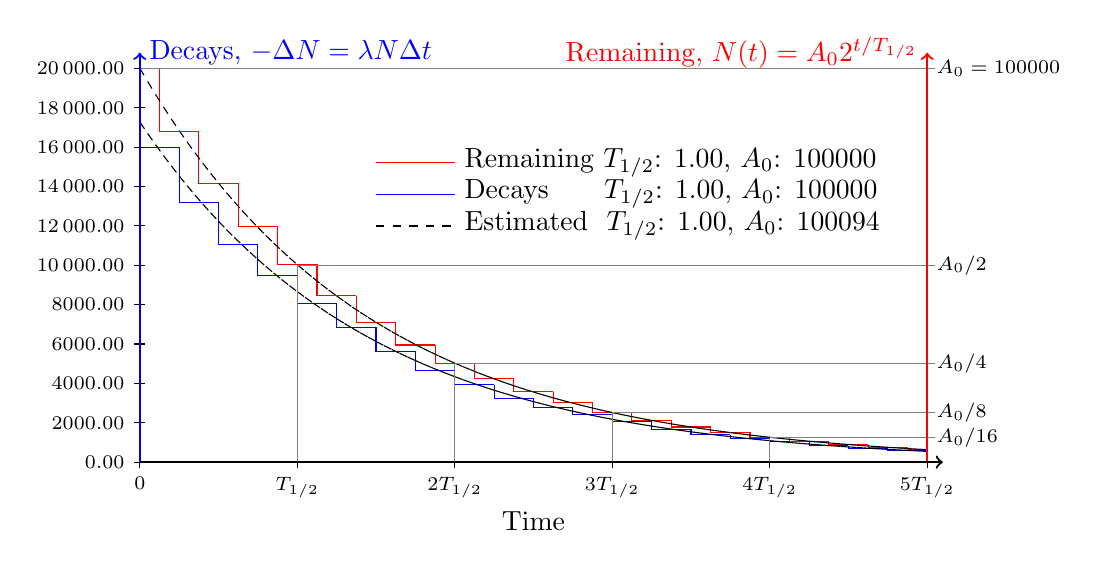
\begin{tikzpicture}
\begin{scope}[]
\clip (0,0) rectangle (10,5);
\begin{scope}[draw=blue]
\draw[] (0.0,3.99825) -- (0.5,3.99825);
\draw (0.5,3.99825) -- (0.5,3.29475) -- (1.0,3.29475);
\draw (1.0,3.29475) -- (1.0,2.769) -- (1.5,2.769);
\draw (1.5,2.769) -- (1.5,2.368) -- (2.0,2.368);
\draw (2.0,2.368) -- (2.0,2.011) -- (2.5,2.011);
\draw (2.5,2.011) -- (2.5,1.71425) -- (3.0,1.71425);
\draw (3.0,1.71425) -- (3.0,1.4085) -- (3.5,1.4085);
\draw (3.5,1.4085) -- (3.5,1.1675) -- (4.0,1.1675);
\draw (4.0,1.1675) -- (4.0,0.984) -- (4.5,0.984);
\draw (4.5,0.984) -- (4.5,0.813) -- (5.0,0.813);
\draw (5.0,0.813) -- (5.0,0.69425) -- (5.5,0.69425);
\draw (5.5,0.69425) -- (5.5,0.60925) -- (6.0,0.60925);
\draw (6.0,0.60925) -- (6.0,0.51625) -- (6.5,0.51625);
\draw (6.5,0.51625) -- (6.5,0.4195) -- (7.0,0.4195);
\draw (7.0,0.4195) -- (7.0,0.347) -- (7.5,0.347);
\draw (7.5,0.347) -- (7.5,0.29825) -- (8.0,0.29825);
\draw (8.0,0.29825) -- (8.0,0.2625) -- (8.5,0.2625);
\draw (8.5,0.2625) -- (8.5,0.2085) -- (9.0,0.2085);
\draw (9.0,0.2085) -- (9.0,0.17825) -- (9.5,0.17825);
\draw (9.5,0.17825) -- (9.5,0.149) -- (10.0,0.149);
\draw (10.0,0.149) -- (10.0,0.12175) -- (10.5,0.12175);
\draw (10.5,0.12175) -- (10.5,0.1085) -- (11.0,0.1085);
\draw (11.0,0.1085) -- (11.0,0.08825) -- (11.5,0.08825);
\draw (11.5,0.08825) -- (11.5,0.072) -- (12.0,0.072);
\draw (12.0,0.072) -- (12.0,0.06375) -- (12.5,0.06375);
\end{scope}
\begin{scope}[draw=red]
\draw[] (-0.25,5.0) -- (0.25,5.0);
\draw (0.25,5.0) -- (0.25,4.20035009765625) -- (0.75,4.20035009765625);
\draw (0.75,4.20035009765625) -- (0.75,3.541400146484375) -- (1.25,3.541400146484375);
\draw (1.25,3.541400146484375) -- (1.25,2.98760009765625) -- (1.75,2.98760009765625);
\draw (1.75,2.98760009765625) -- (1.75,2.514) -- (2.25,2.514);
\draw (2.25,2.514) -- (2.25,2.111800048828125) -- (2.75,2.111800048828125);
\draw (2.75,2.111800048828125) -- (2.75,1.7689500732421874) -- (3.25,1.7689500732421874);
\draw (3.25,1.7689500732421874) -- (3.25,1.48725) -- (3.75,1.48725);
\draw (3.75,1.48725) -- (3.75,1.25375) -- (4.25,1.25375);
\draw (4.25,1.25375) -- (4.25,1.0569500732421875) -- (4.75,1.0569500732421875);
\draw (4.75,1.0569500732421875) -- (4.75,0.8943500366210938) -- (5.25,0.8943500366210938);
\draw (5.25,0.8943500366210938) -- (5.25,0.7555) -- (5.75,0.7555);
\draw (5.75,0.7555) -- (5.75,0.6336500244140625) -- (6.25,0.6336500244140625);
\draw (6.25,0.6336500244140625) -- (6.25,0.5304000244140625) -- (6.75,0.5304000244140625);
\draw (6.75,0.5304000244140625) -- (6.75,0.4465) -- (7.25,0.4465);
\draw (7.25,0.4465) -- (7.25,0.37710000610351563) -- (7.75,0.37710000610351563);
\draw (7.75,0.37710000610351563) -- (7.75,0.31745001220703123) -- (8.25,0.31745001220703123);
\draw (8.25,0.31745001220703123) -- (8.25,0.26495001220703124) -- (8.75,0.26495001220703124);
\draw (8.75,0.26495001220703124) -- (8.75,0.22325) -- (9.25,0.22325);
\draw (9.25,0.22325) -- (9.25,0.18760000610351563) -- (9.75,0.18760000610351563);
\draw (9.75,0.18760000610351563) -- (9.75,0.15780000305175781) -- (10.25,0.15780000305175781);
\draw (10.25,0.15780000305175781) -- (10.25,0.1334499969482422) -- (10.75,0.1334499969482422);
\draw (10.75,0.1334499969482422) -- (10.75,0.11175) -- (11.25,0.11175);
\draw (11.25,0.11175) -- (11.25,0.0940999984741211) -- (11.75,0.0940999984741211);
\draw (11.75,0.0940999984741211) -- (11.75,0.07970000457763672) -- (12.25,0.07970000457763672);
\end{scope}
\begin{scope}[black,dashed]
\draw[] (0.0,4.320596879379904) -- (0.1,4.173944215473551);
\draw[] (0.1,4.173944215473551) -- (0.2,4.032269336912893);
\draw[] (0.2,4.032269336912893) -- (0.3,3.8954032842921604);
\draw[] (0.3,3.8954032842921604) -- (0.4,3.763182833141673);
\draw[] (0.4,3.763182833141673) -- (0.5,3.6354502992686935);
\draw[] (0.5,3.6354502992686935) -- (0.6,3.5120533507055547);
\draw[] (0.6,3.5120533507055547) -- (0.7,3.3928448260407587);
\draw[] (0.7,3.3928448260407587) -- (0.8,3.2776825589164122);
\draw[] (0.8,3.2776825589164122) -- (0.9,3.1664292084826937);
\draw[] (0.9,3.1664292084826937) -- (1.0,3.058952095607142);
\draw[] (1.0,3.058952095607142) -- (1.1,2.9551230446434493);
\draw[] (1.1,2.9551230446434493) -- (1.2,2.854818230571045);
\draw[] (1.2,2.854818230571045) -- (1.3,2.757918031323168);
\draw[] (1.3,2.757918031323168) -- (1.4,2.6643068851273326);
\draw[] (1.4,2.6643068851273326) -- (1.5,2.5738731526880225);
\draw[] (1.5,2.5738731526880225) -- (1.6,2.486508984047296);
\draw[] (1.6,2.486508984047296) -- (1.7,2.402110189964486);
\draw[] (1.7,2.402110189964486) -- (1.8,2.3205761176616226);
\draw[] (1.8,2.3205761176616226) -- (1.9,2.2418095307863894);
\draw[] (1.9,2.2418095307863894) -- (2.0,2.1657164934494597);
\draw[] (2.0,2.1657164934494597) -- (2.1,2.0922062581979195);
\draw[] (2.1,2.0922062581979195) -- (2.2,2.0211911577911668);
\draw[] (2.2,2.0211911577911668) -- (2.3,1.9525865006502348);
\draw[] (2.3,1.9525865006502348) -- (2.4,1.8863104698558417);
\draw[] (2.4,1.8863104698558417) -- (2.5,1.8222840255747204);
\draw[] (2.5,1.8222840255747204) -- (2.6,1.7604308107978583);
\draw[] (2.6,1.7604308107978583) -- (2.7,1.7006770602782357);
\draw[] (2.7,1.7006770602782357) -- (2.8,1.6429515125594625);
\draw[] (2.8,1.6429515125594625) -- (2.9,1.5871853249903976);
\draw[] (2.9,1.5871853249903976) -- (3.0,1.5333119916244022);
\draw[] (3.0,1.5333119916244022) -- (3.1,1.4812672639053133);
\draw[] (3.1,1.4812672639053133) -- (3.2,1.430989074045544);
\draw[] (3.2,1.430989074045544) -- (3.3,1.382417461004944);
\draw[] (3.3,1.382417461004944) -- (3.4,1.3354944989821302);
\draw[] (3.4,1.3354944989821302) -- (3.5,1.290164228333016);
\draw[] (3.5,1.290164228333016) -- (3.6,1.246372588834152);
\draw[] (3.6,1.246372588834152) -- (3.7,1.2040673552112877);
\draw[] (3.7,1.2040673552112877) -- (3.8,1.1631980748562656);
\draw[] (3.8,1.1631980748562656) -- (3.9,1.1237160076579724);
\draw[] (3.9,1.1237160076579724) -- (4.0,1.085574067875591);
\draw[] (4.0,1.085574067875591) -- (4.1,1.048726767984827);
\draw[] (4.1,1.048726767984827) -- (4.2,1.0131301644301465);
\draw[] (4.2,1.0131301644301465) -- (4.3,0.978741805218332);
\draw[] (4.3,0.978741805218332) -- (4.4,0.9455206792908462);
\draw[] (4.4,0.9455206792908462) -- (4.5,0.9134271676146429);
\draw[] (4.5,0.9134271676146429) -- (4.6,0.8824229959330795);
\draw[] (4.6,0.8824229959330795) -- (4.7,0.8524711891205949);
\draw[] (4.7,0.8524711891205949) -- (4.8,0.8235360270867108);
\draw[] (4.8,0.8235360270867108) -- (4.9,0.7955830021767695);
\draw[] (4.9,0.7955830021767695) -- (5.0,0.7685787780186059);
\draw[] (5.0,0.7685787780186059) -- (5.1,0.7424911497660728);
\draw[] (5.1,0.7424911497660728) -- (5.2,0.7172890056920083);
\draw[] (5.2,0.7172890056920083) -- (5.3,0.6929422900848423);
\draw[] (5.3,0.6929422900848423) -- (5.4,0.6694219674045888);
\draw[] (5.4,0.6694219674045888) -- (5.5,0.6466999876554843);
\draw[] (5.5,0.6466999876554843) -- (5.6,0.6247492529339674);
\draw[] (5.6,0.6247492529339674) -- (5.7,0.6035435851121131);
\draw[] (5.7,0.6035435851121131) -- (5.8,0.5830576946179774);
\draw[] (5.8,0.5830576946179774) -- (5.9,0.563267150275619);
\draw[] (5.9,0.563267150275619) -- (6.0,0.544148350168835);
\draw[] (6.0,0.544148350168835) -- (6.1,0.5256784934938564);
\draw[] (6.1,0.5256784934938564) -- (6.2,0.507835553367441);
\draw[] (6.2,0.507835553367441) -- (6.3,0.49059825055793194);
\draw[] (6.3,0.49059825055793194) -- (6.4,0.47394602810795333);
\draw[] (6.4,0.47394602810795333) -- (6.5,0.4578590268184828);
\draw[] (6.5,0.4578590268184828) -- (6.6,0.4423180615650576);
\draw[] (6.6,0.4423180615650576) -- (6.7,0.4273045984178732);
\draw[] (6.7,0.4273045984178732) -- (6.8,0.41280073253848826);
\draw[] (6.8,0.41280073253848826) -- (6.9,0.398789166826773);
\draw[] (6.9,0.398789166826773) -- (7.0,0.38525319129263924);
\draw[] (7.0,0.38525319129263924) -- (7.1,0.3721766631279479);
\draw[] (7.1,0.3721766631279479) -- (7.2,0.35954398745483007);
\draw[] (7.2,0.35954398745483007) -- (7.3,0.34734009872746274);
\draw[] (7.3,0.34734009872746274) -- (7.4,0.335550442765116);
\draw[] (7.4,0.335550442765116) -- (7.5,0.3241609593950491);
\draw[] (7.5,0.3241609593950491) -- (7.6,0.3131580656845519);
\draw[] (7.6,0.3131580656845519) -- (7.7,0.3025286397421364);
\draw[] (7.7,0.3025286397421364) -- (7.8,0.2922600050685593);
\draw[] (7.8,0.2922600050685593) -- (7.9,0.2823399154390125);
\draw[] (7.9,0.2823399154390125) -- (8.0,0.2727565402984537);
\draw[] (8.0,0.2727565402984537) -- (8.1,0.26349845065265703);
\draw[] (8.1,0.26349845065265703) -- (8.2,0.25455460543816094);
\draw[] (8.2,0.25455460543816094) -- (8.3,0.2459143383548557);
\draw[] (8.3,0.2459143383548557) -- (8.4,0.23756734514550923);
\draw[] (8.4,0.23756734514550923) -- (8.5,0.22950367130705826);
\draw[] (8.5,0.22950367130705826) -- (8.6,0.22171370021901302);
\draw[] (8.6,0.22171370021901302) -- (8.7,0.21418814167481504);
\draw[] (8.7,0.21418814167481504) -- (8.8,0.2069180208024712);
\draw[] (8.8,0.2069180208024712) -- (8.9,0.1998946673612523);
\draw[] (8.9,0.1998946673612523) -- (9.0,0.19310970540168873);
\draw[] (9.0,0.19310970540168873) -- (9.1,0.18655504327653508);
\draw[] (9.1,0.18655504327653508) -- (9.2,0.180222863990789);
\draw[] (9.2,0.180222863990789) -- (9.3,0.17410561587925602);
\draw[] (9.3,0.17410561587925602) -- (9.4,0.16819600360054385);
\draw[] (9.4,0.16819600360054385) -- (9.5,0.16248697943674306);
\draw[] (9.5,0.16248697943674306) -- (9.6,0.15697173488842153);
\draw[] (9.6,0.15697173488842153) -- (9.7,0.1516436925549066);
\draw[] (9.7,0.1516436925549066) -- (9.8,0.14649649829017228);
\draw[] (9.8,0.14649649829017228) -- (9.9,0.1415240136249772);
\draw[] (9.9,0.1415240136249772) -- (10.0,0.13672030844621477);
\end{scope}
\begin{scope}[black,dashed]
\draw[] (0.0,5.004728934357686) -- (0.1,4.834854990816327);
\draw[] (0.1,4.834854990816327) -- (0.2,4.670747025227576);
\draw[] (0.2,4.670747025227576) -- (0.3,4.512209324811377);
\draw[] (0.3,4.512209324811377) -- (0.4,4.359052819805141);
\draw[] (0.4,4.359052819805141) -- (0.5,4.211094857981897);
\draw[] (0.5,4.211094857981897) -- (0.6,4.068158986821887);
\draw[] (0.6,4.068158986821887) -- (0.7,3.9300747430778546);
\draw[] (0.7,3.9300747430778546) -- (0.8,3.796677449483049);
\draw[] (0.8,3.796677449483049) -- (0.9,3.6678080183595);
\draw[] (0.9,3.6678080183595) -- (1.0,3.543312761892366);
\draw[] (1.0,3.543312761892366) -- (1.1,3.4230432088440677);
\draw[] (1.1,3.4230432088440677) -- (1.2,3.3068559274896505);
\draw[] (1.2,3.3068559274896505) -- (1.3,3.1946123545621816);
\draw[] (1.3,3.1946123545621816) -- (1.4,3.0861786300042158);
\draw[] (1.4,3.0861786300042158) -- (1.5,2.9814254373282227);
\draw[] (1.5,2.9814254373282227) -- (1.6,2.880227849395627);
\draw[] (1.6,2.880227849395627) -- (1.7,2.7824651794305097);
\draw[] (1.7,2.7824651794305097) -- (1.8,2.6880208370903103);
\draw[] (1.8,2.6880208370903103) -- (1.9,2.5967821894218766);
\draw[] (1.9,2.5967821894218766) -- (2.0,2.508640426537035);
\draw[] (2.0,2.508640426537035) -- (2.1,2.4234904318474983);
\draw[] (2.1,2.4234904318474983) -- (2.2,2.341230656704347);
\draw[] (2.2,2.341230656704347) -- (2.3,2.2617629992925803);
\draw[] (2.3,2.2617629992925803) -- (2.4,2.1849926876363157);
\draw[] (2.4,2.1849926876363157) -- (2.5,2.1108281665751054);
\draw[] (2.5,2.1108281665751054) -- (2.6,2.039180988576581);
\draw[] (2.6,2.039180988576581) -- (2.7,1.9699657082552045);
\draw[] (2.7,1.9699657082552045) -- (2.8,1.9030997804713439);
\draw[] (2.8,1.9030997804713439) -- (2.9,1.8385034618891358);
\draw[] (2.9,1.8385034618891358) -- (3.0,1.7760997158757403);
\draw[] (3.0,1.7760997158757403) -- (3.1,1.715814120628568);
\draw[] (3.1,1.715814120628568) -- (3.2,1.6575747804209182);
\draw[] (3.2,1.6575747804209182) -- (3.3,1.601312239860179);
\draw[] (3.3,1.601312239860179) -- (3.4,1.546959401056331);
\draw[] (3.4,1.546959401056331) -- (3.5,1.494451443601979);
\draw[] (3.5,1.494451443601979) -- (3.6,1.4437257472684712);
\draw[] (3.6,1.4437257472684712) -- (3.7,1.3947218173259264);
\draw[] (3.7,1.3947218173259264) -- (3.8,1.3473812123980926);
\draw[] (3.8,1.3473812123980926) -- (3.9,1.301647474766011);
\draw[] (3.9,1.301647474766011) -- (4.0,1.2574660630373586);
\draw[] (4.0,1.2574660630373586) -- (4.1,1.2147842871011763);
\draw[] (4.1,1.2147842871011763) -- (4.2,1.173551245290403);
\draw[] (4.2,1.173551245290403) -- (4.3,1.1337177636772897);
\draw[] (4.3,1.1337177636772897) -- (4.4,1.0952363374292822);
\draw[] (4.4,1.0952363374292822) -- (4.5,1.0580610741554513);
\draw[] (4.5,1.0580610741554513) -- (4.6,1.0221476391758881);
\draw[] (4.6,1.0221476391758881) -- (4.7,0.9874532026488111);
\draw[] (4.7,0.9874532026488111) -- (4.8,0.9539363884923161);
\draw[] (4.8,0.9539363884923161) -- (4.9,0.9215572250398623);
\draw[] (4.9,0.9215572250398623) -- (5.0,0.8902770973706411);
\draw[] (5.0,0.8902770973706411) -- (5.1,0.8600587012579822);
\draw[] (5.1,0.8600587012579822) -- (5.2,0.8308659986808735);
\draw[] (5.2,0.8308659986808735) -- (5.3,0.8026641748455404);
\draw[] (5.3,0.8026641748455404) -- (5.4,0.7754195966658266);
\draw[] (5.4,0.7754195966658266) -- (5.5,0.7490997726528643);
\draw[] (5.5,0.7490997726528643) -- (5.6,0.7236733141661953);
\draw[] (5.6,0.7236733141661953) -- (5.7,0.6991098979801326);
\draw[] (5.7,0.6991098979801326) -- (5.8,0.6753802301207235);
\draw[] (5.8,0.6753802301207235) -- (5.9,0.6524560109301785);
\draw[] (5.9,0.6524560109301785) -- (6.0,0.6303099013171114);
\draw[] (6.0,0.6303099013171114) -- (6.1,0.6089154901523348);
\draw[] (6.1,0.6089154901523348) -- (6.2,0.5882472627713301);
\draw[] (6.2,0.5882472627713301) -- (6.3,0.5682805705458298);
\draw[] (6.3,0.5682805705458298) -- (6.4,0.5489916014882192);
\draw[] (6.4,0.5489916014882192) -- (6.5,0.5303573518537062);
\draw[] (6.5,0.5303573518537062) -- (6.6,0.5123555987063894);
\draw[] (6.6,0.5123555987063894) -- (6.7,0.49496487341650525);
\draw[] (6.7,0.49496487341650525) -- (6.8,0.4781644360572534);
\draw[] (6.8,0.4781644360572534) -- (6.9,0.4619342506706594);
\draw[] (6.9,0.4619342506706594) -- (7.0,0.44625496137298265);
\draw[] (7.0,0.44625496137298265) -- (7.1,0.43110786927116945);
\draw[] (7.1,0.43110786927116945) -- (7.2,0.41647491016282445);
\draw[] (7.2,0.41647491016282445) -- (7.3,0.40233863299310557);
\draw[] (7.3,0.40233863299310557) -- (7.4,0.3886821790428477);
\draw[] (7.4,0.3886821790428477) -- (7.5,0.3754892618231);
\draw[] (7.5,0.3754892618231) -- (7.6,0.36274414765209434);
\draw[] (7.6,0.36274414765209434) -- (7.7,0.35043163689148527);
\draw[] (7.7,0.35043163689148527) -- (7.8,0.33853704581948146);
\draw[] (7.8,0.33853704581948146) -- (7.9,0.3270461891192516);
\draw[] (7.9,0.3270461891192516) -- (8.0,0.31594536296172254);
\draw[] (8.0,0.31594536296172254) -- (8.1,0.30522132866258983);
\draw[] (8.1,0.30522132866258983) -- (8.2,0.2948612968940557);
\draw[] (8.2,0.2948612968940557) -- (8.3,0.2848529124324621);
\draw[] (8.3,0.2848529124324621) -- (8.4,0.27518423942363024);
\draw[] (8.4,0.27518423942363024) -- (8.5,0.26584374714833364);
\draw[] (8.5,0.26584374714833364) -- (8.6,0.2568202962709296);
\draw[] (8.6,0.2568202962709296) -- (8.7,0.24810312555474928);
\draw[] (8.7,0.24810312555474928) -- (8.8,0.23968183902840276);
\draw[] (8.8,0.23968183902840276) -- (8.9,0.2315463935876947);
\draw[] (8.9,0.2315463935876947) -- (9.0,0.2236870870183631);
\draw[] (9.0,0.2236870870183631) -- (9.1,0.21609454642535988);
\draw[] (9.1,0.21609454642535988) -- (9.2,0.20875971705487203);
\draw[] (9.2,0.20875971705487203) -- (9.3,0.20167385149575326);
\draw[] (9.3,0.20167385149575326) -- (9.4,0.19482849924748913);
\draw[] (9.4,0.19482849924748913) -- (9.5,0.18821549664225148);
\draw[] (9.5,0.18821549664225148) -- (9.6,0.18182695710902738);
\draw[] (9.6,0.18182695710902738) -- (9.7,0.17565526176820861);
\draw[] (9.7,0.17565526176820861) -- (9.8,0.16969305034542645);
\draw[] (9.8,0.16969305034542645) -- (9.9,0.1639332123937953);
\draw[] (9.9,0.1639332123937953) -- (10.0,0.15836887881409628);
\end{scope}
\draw[blue] (3.0,3.4) -- (4.0,3.4);
\node[right,] at (4.0,3.4) {Decays\ \ \ \ \ \ $T_{1/2}$:  1.00, $A_0$: 100000};
\draw[black,thick,dashed] (3.0,3.0) -- (4.0,3.0);
\node[right,] at (4.0,3.0) {Estimated \ $T_{1/2}$:  1.00, $A_0$: 100094};
\draw[red] (3.0,3.8) -- (4.0,3.8);
\node[right,] at (4.0,3.8) {Remaining $T_{1/2}$:  1.00, $A_0$: 100000};
\end{scope}
\draw (0,0cm + 2pt) -- (0, 0cm-2pt) node[below] {\scriptsize $0$};
\draw (2,0cm + 2pt) -- (2, 0cm-2pt) node[below] {\scriptsize $T_{1/2}$};
\draw (4,0cm + 2pt) -- (4, 0cm-2pt) node[below] {\scriptsize $2T_{1/2}$};
\draw (6,0cm + 2pt) -- (6, 0cm-2pt) node[below] {\scriptsize $3T_{1/2}$};
\draw (8,0cm + 2pt) -- (8, 0cm-2pt) node[below] {\scriptsize $4T_{1/2}$};
\draw (10,0cm + 2pt) -- (10, 0cm-2pt) node[below] {\scriptsize $5T_{1/2}$};
\draw (0cm + 2pt,0.    ) -- (0cm-2pt,0.    ) node[left] {\scriptsize{\num[round-mode=places,round-precision=2]{0}}};
\draw (0cm + 2pt,0.5    ) -- (0cm-2pt,0.5    ) node[left] {\scriptsize{\num[round-mode=places,round-precision=2]{2000}}};
\draw (0cm + 2pt,1.    ) -- (0cm-2pt,1.    ) node[left] {\scriptsize{\num[round-mode=places,round-precision=2]{4000}}};
\draw (0cm + 2pt,1.5    ) -- (0cm-2pt,1.5    ) node[left] {\scriptsize{\num[round-mode=places,round-precision=2]{6000}}};
\draw (0cm + 2pt,2.    ) -- (0cm-2pt,2.    ) node[left] {\scriptsize{\num[round-mode=places,round-precision=2]{8000}}};
\draw (0cm + 2pt,2.5    ) -- (0cm-2pt,2.5    ) node[left] {\scriptsize{\num[round-mode=places,round-precision=2]{10000}}};
\draw (0cm + 2pt,3.    ) -- (0cm-2pt,3.    ) node[left] {\scriptsize{\num[round-mode=places,round-precision=2]{12000}}};
\draw (0cm + 2pt,3.5    ) -- (0cm-2pt,3.5    ) node[left] {\scriptsize{\num[round-mode=places,round-precision=2]{14000}}};
\draw (0cm + 2pt,4.    ) -- (0cm-2pt,4.    ) node[left] {\scriptsize{\num[round-mode=places,round-precision=2]{16000}}};
\draw (0cm + 2pt,4.5    ) -- (0cm-2pt,4.5    ) node[left] {\scriptsize{\num[round-mode=places,round-precision=2]{18000}}};
\draw (0cm + 2pt,5.    ) -- (0cm-2pt,5.    ) node[left] {\scriptsize{\num[round-mode=places,round-precision=2]{20000}}};
\draw[thin,gray] (0.0,5.0) -- (10.1,5.0);
\node[right] at (10.0,5.0) {\scriptsize{$A_0 = 100000$}};
\draw[thin,gray] (2.0,2.5) -- (10.1,2.5);
\draw[thin,gray] (2.0,0.0) -- (2.0,2.5);
\node[right] at (10.0,2.5) {\scriptsize{$A_0/2$}};
\draw[thin,gray] (4.0,1.25) -- (10.1,1.25);
\draw[thin,gray] (4.0,0.0) -- (4.0,1.25);
\node[right] at (10.0,1.25) {\scriptsize{$A_0/4$}};
\draw[thin,gray] (6.0,0.625) -- (10.1,0.625);
\draw[thin,gray] (6.0,0.0) -- (6.0,0.625);
\node[right] at (10.0,0.625) {\scriptsize{$A_0/8$}};
\draw[thin,gray] (8.0,0.3125) -- (10.1,0.3125);
\draw[thin,gray] (8.0,0.0) -- (8.0,0.3125);
\node[right] at (10.0,0.3125) {\scriptsize{$A_0/16$}};
\node[right,blue] at (0.0,5.2) {Decays, $-\Delta N = \lambda N \Delta t$};
\node[left,red] at (10.0,5.2) {Remaining, $N(t) = A_0 2^{t/T_{1/2}}$};
\node[below] at (5.0,-0.5) {Time};
\draw[blue,thick,->] (0.0,0.0) -- (0.0,5.2);
\draw[red,thick,->] (10.0,0.0) -- (10.0,5.2);
\draw[thick,->] (0.0,0.0) -- (10.2,0.0);
\end{tikzpicture}
%%% Local Variables: 
%%% mode: latex 
%%% TeX-master: "master" 
%%% End:


  \caption{ Attempt to show all data in one plot.}
\end{figure}

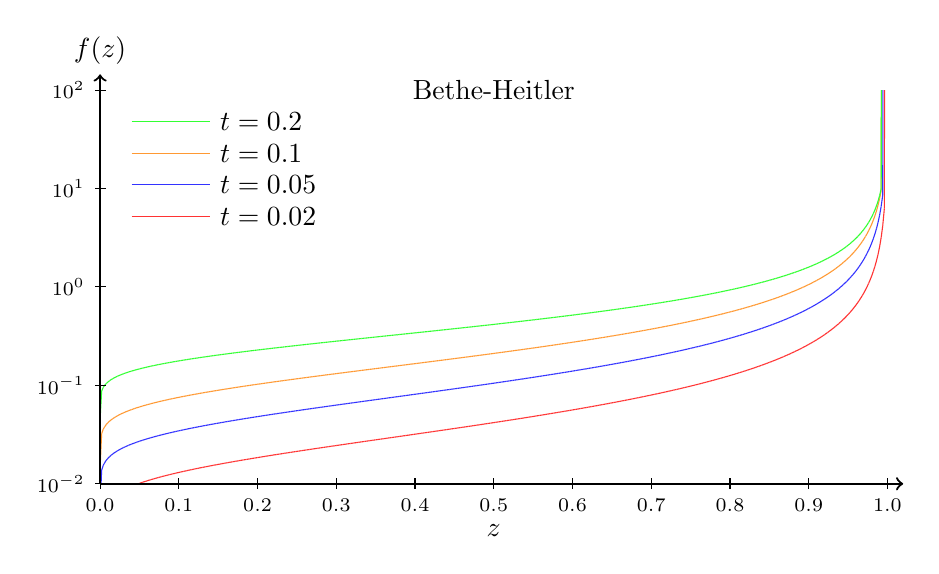
\begin{tikzpicture}
\begin{scope}[]
\clip (0,0) rectangle (10,5);
\begin{scope}[red!80]
\draw[] (0.000001,-0.88166773) -- (0.020000994,-0.37921697);
\draw[] (0.020000994,-0.37921697) -- (0.040000994,-0.3168717);
\draw[] (0.040000994,-0.3168717) -- (0.060000993,-0.2766621);
\draw[] (0.060000993,-0.2766621) -- (0.08000098,-0.24615079);
\draw[] (0.08000098,-0.24615079) -- (0.10000098,-0.22120506);
\draw[] (0.10000098,-0.22120506) -- (0.12000098,-0.19990832);
\draw[] (0.12000098,-0.19990832) -- (0.14000097,-0.18120557);
\draw[] (0.14000097,-0.18120557) -- (0.16000098,-0.1644504);
\draw[] (0.16000098,-0.1644504) -- (0.18000098,-0.14921606);
\draw[] (0.18000098,-0.14921606) -- (0.20000096,-0.13520539);
\draw[] (0.20000096,-0.13520539) -- (0.22000097,-0.12220144);
\draw[] (0.22000097,-0.12220144) -- (0.24000096,-0.110043585);
\draw[] (0.24000096,-0.110043585) -- (0.26000094,-0.09860605);
\draw[] (0.26000094,-0.09860605) -- (0.28000095,-0.087791085);
\draw[] (0.28000095,-0.087791085) -- (0.30000094,-0.07751852);
\draw[] (0.30000094,-0.07751852) -- (0.32000095,-0.06772518);
\draw[] (0.32000095,-0.06772518) -- (0.34000096,-0.05835682);
\draw[] (0.34000096,-0.05835682) -- (0.36000094,-0.04936874);
\draw[] (0.36000094,-0.04936874) -- (0.38000092,-0.04072368);
\draw[] (0.38000092,-0.04072368) -- (0.40000093,-0.032388866);
\draw[] (0.40000093,-0.032388866) -- (0.4200009,-0.024336576);
\draw[] (0.4200009,-0.024336576) -- (0.44000092,-0.016542673);
\draw[] (0.44000092,-0.016542673) -- (0.46000093,-0.008985996);
\draw[] (0.46000093,-0.008985996) -- (0.48000094,-0.0016480684);
\draw[] (0.48000094,-0.0016480684) -- (0.5000009,0.0054873526);
\draw[] (0.5000009,0.0054873526) -- (0.5200009,0.012435168);
\draw[] (0.5200009,0.012435168) -- (0.5400009,0.01920849);
\draw[] (0.5400009,0.01920849) -- (0.5600009,0.025818646);
\draw[] (0.5600009,0.025818646) -- (0.5800009,0.032276213);
\draw[] (0.5800009,0.032276213) -- (0.60000086,0.038591027);
\draw[] (0.60000086,0.038591027) -- (0.6200009,0.044771582);
\draw[] (0.6200009,0.044771582) -- (0.6400008,0.050825775);
\draw[] (0.6400008,0.050825775) -- (0.6600008,0.05676061);
\draw[] (0.6600008,0.05676061) -- (0.68000084,0.06258324);
\draw[] (0.68000084,0.06258324) -- (0.7000008,0.06829888);
\draw[] (0.7000008,0.06829888) -- (0.72000086,0.073913485);
\draw[] (0.72000086,0.073913485) -- (0.74000084,0.07943243);
\draw[] (0.74000084,0.07943243) -- (0.76000077,0.084860176);
\draw[] (0.76000077,0.084860176) -- (0.7800008,0.0902012);
\draw[] (0.7800008,0.0902012) -- (0.8000008,0.09545937);
\draw[] (0.8000008,0.09545937) -- (0.8200008,0.100639015);
\draw[] (0.8200008,0.100639015) -- (0.8400008,0.10574341);
\draw[] (0.8400008,0.10574341) -- (0.8600008,0.11077568);
\draw[] (0.8600008,0.11077568) -- (0.8800008,0.11573896);
\draw[] (0.8800008,0.11573896) -- (0.90000075,0.120636374);
\draw[] (0.90000075,0.120636374) -- (0.9200008,0.1254709);
\draw[] (0.9200008,0.1254709) -- (0.9400008,0.1302442);
\draw[] (0.9400008,0.1302442) -- (0.9600008,0.13495967);
\draw[] (0.9600008,0.13495967) -- (0.9800008,0.13961881);
\draw[] (0.9800008,0.13961881) -- (1.0000007,0.14422446);
\draw[] (1.0000007,0.14422446) -- (1.0200008,0.14877811);
\draw[] (1.0200008,0.14877811) -- (1.0400008,0.15328169);
\draw[] (1.0400008,0.15328169) -- (1.0600008,0.15773743);
\draw[] (1.0600008,0.15773743) -- (1.0800008,0.16214654);
\draw[] (1.0800008,0.16214654) -- (1.1000007,0.16651124);
\draw[] (1.1000007,0.16651124) -- (1.1200007,0.17083257);
\draw[] (1.1200007,0.17083257) -- (1.1400007,0.17511234);
\draw[] (1.1400007,0.17511234) -- (1.1600008,0.17935172);
\draw[] (1.1600008,0.17935172) -- (1.1800008,0.18355191);
\draw[] (1.1800008,0.18355191) -- (1.2000006,0.1877144);
\draw[] (1.2000006,0.1877144) -- (1.2200007,0.19184068);
\draw[] (1.2200007,0.19184068) -- (1.2400007,0.19593135);
\draw[] (1.2400007,0.19593135) -- (1.2600007,0.19998804);
\draw[] (1.2600007,0.19998804) -- (1.2800008,0.2040115);
\draw[] (1.2800008,0.2040115) -- (1.3000008,0.20800263);
\draw[] (1.3000008,0.20800263) -- (1.3200008,0.21196261);
\draw[] (1.3200008,0.21196261) -- (1.3400007,0.21589234);
\draw[] (1.3400007,0.21589234) -- (1.3600008,0.21979287);
\draw[] (1.3600008,0.21979287) -- (1.3800008,0.22366464);
\draw[] (1.3800008,0.22366464) -- (1.4000007,0.22750899);
\draw[] (1.4000007,0.22750899) -- (1.4200008,0.23132637);
\draw[] (1.4200008,0.23132637) -- (1.4400008,0.23511738);
\draw[] (1.4400008,0.23511738) -- (1.4600008,0.2388832);
\draw[] (1.4600008,0.2388832) -- (1.4800007,0.24262428);
\draw[] (1.4800007,0.24262428) -- (1.5000008,0.24634153);
\draw[] (1.5000008,0.24634153) -- (1.5200007,0.25003523);
\draw[] (1.5200007,0.25003523) -- (1.5400007,0.25370598);
\draw[] (1.5400007,0.25370598) -- (1.5600008,0.25735497);
\draw[] (1.5600008,0.25735497) -- (1.5800008,0.26098236);
\draw[] (1.5800008,0.26098236) -- (1.6000007,0.26458845);
\draw[] (1.6000007,0.26458845) -- (1.6200007,0.26817456);
\draw[] (1.6200007,0.26817456) -- (1.6400008,0.27174056);
\draw[] (1.6400008,0.27174056) -- (1.6600007,0.27528718);
\draw[] (1.6600007,0.27528718) -- (1.6800007,0.27881518);
\draw[] (1.6800007,0.27881518) -- (1.7000008,0.28232425);
\draw[] (1.7000008,0.28232425) -- (1.7200006,0.28581575);
\draw[] (1.7200006,0.28581575) -- (1.7400007,0.28928965);
\draw[] (1.7400007,0.28928965) -- (1.7600007,0.29274672);
\draw[] (1.7600007,0.29274672) -- (1.7800008,0.29618666);
\draw[] (1.7800008,0.29618666) -- (1.8000007,0.29961094);
\draw[] (1.8000007,0.29961094) -- (1.8200006,0.30301914);
\draw[] (1.8200006,0.30301914) -- (1.8400007,0.30641168);
\draw[] (1.8400007,0.30641168) -- (1.8600006,0.30978948);
\draw[] (1.8600006,0.30978948) -- (1.8800007,0.31315267);
\draw[] (1.8800007,0.31315267) -- (1.9000007,0.31650126);
\draw[] (1.9000007,0.31650126) -- (1.9200008,0.31983584);
\draw[] (1.9200008,0.31983584) -- (1.9400007,0.32315686);
\draw[] (1.9400007,0.32315686) -- (1.9600006,0.32646447);
\draw[] (1.9600006,0.32646447) -- (1.9800007,0.32975912);
\draw[] (1.9800007,0.32975912) -- (2.0000005,0.33304125);
\draw[] (2.0000005,0.33304125) -- (2.0200007,0.33631057);
\draw[] (2.0200007,0.33631057) -- (2.0400007,0.3395681);
\draw[] (2.0400007,0.3395681) -- (2.0600007,0.34281388);
\draw[] (2.0600007,0.34281388) -- (2.0800006,0.34604773);
\draw[] (2.0800006,0.34604773) -- (2.1000006,0.3492707);
\draw[] (2.1000006,0.3492707) -- (2.1200006,0.35248235);
\draw[] (2.1200006,0.35248235) -- (2.1400006,0.35568342);
\draw[] (2.1400006,0.35568342) -- (2.1600006,0.35887405);
\draw[] (2.1600006,0.35887405) -- (2.1800005,0.3620544);
\draw[] (2.1800005,0.3620544) -- (2.2000005,0.36522448);
\draw[] (2.2000005,0.36522448) -- (2.2200005,0.36838517);
\draw[] (2.2200005,0.36838517) -- (2.2400007,0.37153617);
\draw[] (2.2400007,0.37153617) -- (2.2600005,0.37467778);
\draw[] (2.2600005,0.37467778) -- (2.2800004,0.3778103);
\draw[] (2.2800004,0.3778103) -- (2.3000007,0.38093403);
\draw[] (2.3000007,0.38093403) -- (2.3200006,0.38404897);
\draw[] (2.3200006,0.38404897) -- (2.3400006,0.38715556);
\draw[] (2.3400006,0.38715556) -- (2.3600006,0.3902538);
\draw[] (2.3600006,0.3902538) -- (2.3800006,0.39334416);
\draw[] (2.3800006,0.39334416) -- (2.4000006,0.39642632);
\draw[] (2.4000006,0.39642632) -- (2.4200006,0.39950117);
\draw[] (2.4200006,0.39950117) -- (2.4400005,0.40256828);
\draw[] (2.4400005,0.40256828) -- (2.4600005,0.40562823);
\draw[] (2.4600005,0.40562823) -- (2.4800005,0.4086809);
\draw[] (2.4800005,0.4086809) -- (2.5000005,0.41172683);
\draw[] (2.5000005,0.41172683) -- (2.5200002,0.41476563);
\draw[] (2.5200002,0.41476563) -- (2.5400004,0.41779816);
\draw[] (2.5400004,0.41779816) -- (2.5600004,0.420824);
\draw[] (2.5600004,0.420824) -- (2.5800004,0.4238437);
\draw[] (2.5800004,0.4238437) -- (2.6000004,0.42685732);
\draw[] (2.6000004,0.42685732) -- (2.6200006,0.42986497);
\draw[] (2.6200006,0.42986497) -- (2.6400003,0.4328665);
\draw[] (2.6400003,0.4328665) -- (2.6600003,0.4358627);
\draw[] (2.6600003,0.4358627) -- (2.6800003,0.43885335);
\draw[] (2.6800003,0.43885335) -- (2.7000003,0.4418385);
\draw[] (2.7000003,0.4418385) -- (2.7200005,0.4448186);
\draw[] (2.7200005,0.4448186) -- (2.7400005,0.4477936);
\draw[] (2.7400005,0.4477936) -- (2.7600005,0.45076355);
\draw[] (2.7600005,0.45076355) -- (2.7800002,0.45372874);
\draw[] (2.7800002,0.45372874) -- (2.8000002,0.4566893);
\draw[] (2.8000002,0.4566893) -- (2.8200004,0.45964524);
\draw[] (2.8200004,0.45964524) -- (2.8400004,0.46259686);
\draw[] (2.8400004,0.46259686) -- (2.8600004,0.4655443);
\draw[] (2.8600004,0.4655443) -- (2.8800004,0.46848744);
\draw[] (2.8800004,0.46848744) -- (2.9,0.47142655);
\draw[] (2.9,0.47142655) -- (2.9200003,0.47436178);
\draw[] (2.9200003,0.47436178) -- (2.9400003,0.47729343);
\draw[] (2.9400003,0.47729343) -- (2.9600003,0.4802212);
\draw[] (2.9600003,0.4802212) -- (2.9800003,0.48314556);
\draw[] (2.9800003,0.48314556) -- (3.0000005,0.4860665);
\draw[] (3.0000005,0.4860665) -- (3.0200005,0.48898414);
\draw[] (3.0200005,0.48898414) -- (3.0400002,0.4918985);
\draw[] (3.0400002,0.4918985) -- (3.0600002,0.4948099);
\draw[] (3.0600002,0.4948099) -- (3.0800002,0.4977183);
\draw[] (3.0800002,0.4977183) -- (3.1000004,0.5006239);
\draw[] (3.1000004,0.5006239) -- (3.1200004,0.5035266);
\draw[] (3.1200004,0.5035266) -- (3.1400003,0.5064268);
\draw[] (3.1400003,0.5064268) -- (3.1600003,0.5093245);
\draw[] (3.1600003,0.5093245) -- (3.18,0.5122198);
\draw[] (3.18,0.5122198) -- (3.2000003,0.5151126);
\draw[] (3.2000003,0.5151126) -- (3.2200003,0.5180034);
\draw[] (3.2200003,0.5180034) -- (3.2400002,0.52089214);
\draw[] (3.2400002,0.52089214) -- (3.2600002,0.5237786);
\draw[] (3.2600002,0.5237786) -- (3.2800004,0.52666336);
\draw[] (3.2800004,0.52666336) -- (3.3000004,0.52954626);
\draw[] (3.3000004,0.52954626) -- (3.3200002,0.53242743);
\draw[] (3.3200002,0.53242743) -- (3.3400002,0.53530693);
\draw[] (3.3400002,0.53530693) -- (3.3600001,0.53818494);
\draw[] (3.3600001,0.53818494) -- (3.3800004,0.5410616);
\draw[] (3.3800004,0.5410616) -- (3.4000003,0.5439368);
\draw[] (3.4000003,0.5439368) -- (3.4200003,0.5468109);
\draw[] (3.4200003,0.5468109) -- (3.44,0.5496837);
\draw[] (3.44,0.5496837) -- (3.46,0.5525556);
\draw[] (3.46,0.5525556) -- (3.4800003,0.5554265);
\draw[] (3.4800003,0.5554265) -- (3.5000002,0.55829656);
\draw[] (3.5000002,0.55829656) -- (3.5200002,0.5611658);
\draw[] (3.5200002,0.5611658) -- (3.5400002,0.5640344);
\draw[] (3.5400002,0.5640344) -- (3.5600004,0.56690246);
\draw[] (3.5600004,0.56690246) -- (3.5800002,0.56976986);
\draw[] (3.5800002,0.56976986) -- (3.6000001,0.57263684);
\draw[] (3.6000001,0.57263684) -- (3.6200001,0.5755035);
\draw[] (3.6200001,0.5755035) -- (3.64,0.5783699);
\draw[] (3.64,0.5783699) -- (3.6600003,0.5812363);
\draw[] (3.6600003,0.5812363) -- (3.6800003,0.5841026);
\draw[] (3.6800003,0.5841026) -- (3.7000003,0.58696866);
\draw[] (3.7000003,0.58696866) -- (3.72,0.58983487);
\draw[] (3.72,0.58983487) -- (3.74,0.59270126);
\draw[] (3.74,0.59270126) -- (3.7600002,0.59556794);
\draw[] (3.7600002,0.59556794) -- (3.7800002,0.5984351);
\draw[] (3.7800002,0.5984351) -- (3.8000002,0.6013025);
\draw[] (3.8000002,0.6013025) -- (3.8200002,0.60417056);
\draw[] (3.8200002,0.60417056) -- (3.8400004,0.60703933);
\draw[] (3.8400004,0.60703933) -- (3.8600001,0.6099084);
\draw[] (3.8600001,0.6099084) -- (3.88,0.6127785);
\draw[] (3.88,0.6127785) -- (3.9,0.6156492);
\draw[] (3.9,0.6156492) -- (3.92,0.618521);
\draw[] (3.92,0.618521) -- (3.9400003,0.62139374);
\draw[] (3.9400003,0.62139374) -- (3.9600003,0.6242676);
\draw[] (3.9600003,0.6242676) -- (3.98,0.6271425);
\draw[] (3.98,0.6271425) -- (4.0,0.6300187);
\draw[] (4.0,0.6300187) -- (4.02,0.6328961);
\draw[] (4.02,0.6328961) -- (4.04,0.635775);
\draw[] (4.04,0.635775) -- (4.06,0.6386554);
\draw[] (4.06,0.6386554) -- (4.08,0.6415373);
\draw[] (4.08,0.6415373) -- (4.1000004,0.644421);
\draw[] (4.1000004,0.644421) -- (4.12,0.64730614);
\draw[] (4.12,0.64730614) -- (4.14,0.6501932);
\draw[] (4.14,0.6501932) -- (4.16,0.65308213);
\draw[] (4.16,0.65308213) -- (4.18,0.6559731);
\draw[] (4.18,0.6559731) -- (4.2000003,0.658866);
\draw[] (4.2000003,0.658866) -- (4.2200003,0.66176087);
\draw[] (4.2200003,0.66176087) -- (4.2400002,0.66465825);
\draw[] (4.2400002,0.66465825) -- (4.2599998,0.6675577);
\draw[] (4.2599998,0.6675577) -- (4.2799997,0.6704594);
\draw[] (4.2799997,0.6704594) -- (4.3,0.6733636);
\draw[] (4.3,0.6733636) -- (4.32,0.6762704);
\draw[] (4.32,0.6762704) -- (4.34,0.67917955);
\draw[] (4.34,0.67917955) -- (4.36,0.68209153);
\draw[] (4.36,0.68209153) -- (4.3799996,0.6850062);
\draw[] (4.3799996,0.6850062) -- (4.4,0.6879237);
\draw[] (4.4,0.6879237) -- (4.42,0.69084406);
\draw[] (4.42,0.69084406) -- (4.44,0.6937675);
\draw[] (4.44,0.6937675) -- (4.46,0.69669396);
\draw[] (4.46,0.69669396) -- (4.48,0.69962335);
\draw[] (4.48,0.69962335) -- (4.5,0.7025562);
\draw[] (4.5,0.7025562) -- (4.52,0.7054922);
\draw[] (4.52,0.7054922) -- (4.54,0.7084316);
\draw[] (4.54,0.7084316) -- (4.56,0.7113744);
\draw[] (4.56,0.7113744) -- (4.58,0.71432084);
\draw[] (4.58,0.71432084) -- (4.6,0.717271);
\draw[] (4.6,0.717271) -- (4.62,0.7202247);
\draw[] (4.62,0.7202247) -- (4.64,0.72318226);
\draw[] (4.64,0.72318226) -- (4.66,0.7261434);
\draw[] (4.66,0.7261434) -- (4.68,0.72910875);
\draw[] (4.68,0.72910875) -- (4.7,0.73207796);
\draw[] (4.7,0.73207796) -- (4.72,0.73505133);
\draw[] (4.72,0.73505133) -- (4.74,0.738029);
\draw[] (4.74,0.738029) -- (4.76,0.7410107);
\draw[] (4.76,0.7410107) -- (4.78,0.7439969);
\draw[] (4.78,0.7439969) -- (4.7999997,0.7469876);
\draw[] (4.7999997,0.7469876) -- (4.8199997,0.7499827);
\draw[] (4.8199997,0.7499827) -- (4.8399997,0.7529825);
\draw[] (4.8399997,0.7529825) -- (4.86,0.755987);
\draw[] (4.86,0.755987) -- (4.88,0.7589963);
\draw[] (4.88,0.7589963) -- (4.9,0.76201034);
\draw[] (4.9,0.76201034) -- (4.9199996,0.7650293);
\draw[] (4.9199996,0.7650293) -- (4.9399996,0.76805353);
\draw[] (4.9399996,0.76805353) -- (4.96,0.77108264);
\draw[] (4.96,0.77108264) -- (4.98,0.77411693);
\draw[] (4.98,0.77411693) -- (5.0,0.7771568);
\draw[] (5.0,0.7771568) -- (5.0200005,0.78020185);
\draw[] (5.0200005,0.78020185) -- (5.04,0.7832524);
\draw[] (5.04,0.7832524) -- (5.0600004,0.78630865);
\draw[] (5.0600004,0.78630865) -- (5.08,0.78937036);
\draw[] (5.08,0.78937036) -- (5.1000004,0.7924381);
\draw[] (5.1000004,0.7924381) -- (5.1200004,0.7955114);
\draw[] (5.1200004,0.7955114) -- (5.14,0.7985906);
\draw[] (5.14,0.7985906) -- (5.1600003,0.80167603);
\draw[] (5.1600003,0.80167603) -- (5.18,0.80476743);
\draw[] (5.18,0.80476743) -- (5.2000003,0.80786526);
\draw[] (5.2000003,0.80786526) -- (5.2200003,0.810969);
\draw[] (5.2200003,0.810969) -- (5.2400002,0.81407946);
\draw[] (5.2400002,0.81407946) -- (5.26,0.8171965);
\draw[] (5.26,0.8171965) -- (5.2799997,0.82031995);
\draw[] (5.2799997,0.82031995) -- (5.3,0.8234501);
\draw[] (5.3,0.8234501) -- (5.32,0.8265871);
\draw[] (5.32,0.8265871) -- (5.34,0.82973105);
\draw[] (5.34,0.82973105) -- (5.36,0.8328819);
\draw[] (5.36,0.8328819) -- (5.3800006,0.8360401);
\draw[] (5.3800006,0.8360401) -- (5.4,0.8392052);
\draw[] (5.4,0.8392052) -- (5.42,0.84237766);
\draw[] (5.42,0.84237766) -- (5.44,0.84555775);
\draw[] (5.44,0.84555775) -- (5.46,0.8487451);
\draw[] (5.46,0.8487451) -- (5.4800005,0.8519402);
\draw[] (5.4800005,0.8519402) -- (5.5,0.8551431);
\draw[] (5.5,0.8551431) -- (5.5200005,0.8583537);
\draw[] (5.5200005,0.8583537) -- (5.54,0.8615723);
\draw[] (5.54,0.8615723) -- (5.56,0.864799);
\draw[] (5.56,0.864799) -- (5.5800004,0.86803406);
\draw[] (5.5800004,0.86803406) -- (5.6,0.87127715);
\draw[] (5.6,0.87127715) -- (5.6200004,0.8745287);
\draw[] (5.6200004,0.8745287) -- (5.64,0.8777888);
\draw[] (5.64,0.8777888) -- (5.66,0.8810575);
\draw[] (5.66,0.8810575) -- (5.6800003,0.88433486);
\draw[] (5.6800003,0.88433486) -- (5.7,0.88762134);
\draw[] (5.7,0.88762134) -- (5.7200003,0.8909167);
\draw[] (5.7200003,0.8909167) -- (5.74,0.89422107);
\draw[] (5.74,0.89422107) -- (5.76,0.8975348);
\draw[] (5.76,0.8975348) -- (5.78,0.90085787);
\draw[] (5.78,0.90085787) -- (5.7999997,0.90419054);
\draw[] (5.7999997,0.90419054) -- (5.82,0.9075327);
\draw[] (5.82,0.9075327) -- (5.8399997,0.91088456);
\draw[] (5.8399997,0.91088456) -- (5.86,0.91424644);
\draw[] (5.86,0.91424644) -- (5.88,0.9176183);
\draw[] (5.88,0.9176183) -- (5.9,0.92100024);
\draw[] (5.9,0.92100024) -- (5.92,0.92439234);
\draw[] (5.92,0.92439234) -- (5.9399996,0.927795);
\draw[] (5.9399996,0.927795) -- (5.96,0.93120825);
\draw[] (5.96,0.93120825) -- (5.98,0.9346321);
\draw[] (5.98,0.9346321) -- (6.0,0.93806696);
\draw[] (6.0,0.93806696) -- (6.02,0.9415126);
\draw[] (6.02,0.9415126) -- (6.0400004,0.94496965);
\draw[] (6.0400004,0.94496965) -- (6.06,0.9484376);
\draw[] (6.06,0.9484376) -- (6.08,0.9519172);
\draw[] (6.08,0.9519172) -- (6.1,0.95540833);
\draw[] (6.1,0.95540833) -- (6.12,0.9589112);
\draw[] (6.12,0.9589112) -- (6.1400003,0.9624259);
\draw[] (6.1400003,0.9624259) -- (6.16,0.9659526);
\draw[] (6.16,0.9659526) -- (6.1800003,0.9694917);
\draw[] (6.1800003,0.9694917) -- (6.2,0.97304296);
\draw[] (6.2,0.97304296) -- (6.22,0.9766069);
\draw[] (6.22,0.9766069) -- (6.2400002,0.9801836);
\draw[] (6.2400002,0.9801836) -- (6.2599998,0.983773);
\draw[] (6.2599998,0.983773) -- (6.28,0.9873755);
\draw[] (6.28,0.9873755) -- (6.2999997,0.9909911);
\draw[] (6.2999997,0.9909911) -- (6.32,0.9946203);
\draw[] (6.32,0.9946203) -- (6.34,0.9982629);
\draw[] (6.34,0.9982629) -- (6.3599997,1.0019194);
\draw[] (6.3599997,1.0019194) -- (6.38,1.0055896);
\draw[] (6.38,1.0055896) -- (6.3999996,1.0092741);
\draw[] (6.3999996,1.0092741) -- (6.42,1.0129731);
\draw[] (6.42,1.0129731) -- (6.44,1.0166862);
\draw[] (6.44,1.0166862) -- (6.46,1.0204144);
\draw[] (6.46,1.0204144) -- (6.48,1.024157);
\draw[] (6.48,1.024157) -- (6.4999995,1.0279151);
\draw[] (6.4999995,1.0279151) -- (6.52,1.0316885);
\draw[] (6.52,1.0316885) -- (6.54,1.0354772);
\draw[] (6.54,1.0354772) -- (6.56,1.039282);
\draw[] (6.56,1.039282) -- (6.58,1.0431024);
\draw[] (6.58,1.0431024) -- (6.6000004,1.046939);
\draw[] (6.6000004,1.046939) -- (6.62,1.0507922);
\draw[] (6.62,1.0507922) -- (6.64,1.0546618);
\draw[] (6.64,1.0546618) -- (6.66,1.0585483);
\draw[] (6.66,1.0585483) -- (6.68,1.0624521);
\draw[] (6.68,1.0624521) -- (6.7000003,1.066373);
\draw[] (6.7000003,1.066373) -- (6.72,1.0703113);
\draw[] (6.72,1.0703113) -- (6.74,1.0742676);
\draw[] (6.74,1.0742676) -- (6.7599998,1.0782421);
\draw[] (6.7599998,1.0782421) -- (6.7799997,1.0822345);
\draw[] (6.7799997,1.0822345) -- (6.8,1.086246);
\draw[] (6.8,1.086246) -- (6.8199997,1.0902759);
\draw[] (6.8199997,1.0902759) -- (6.84,1.0943253);
\draw[] (6.84,1.0943253) -- (6.8599997,1.0983938);
\draw[] (6.8599997,1.0983938) -- (6.8799996,1.102482);
\draw[] (6.8799996,1.102482) -- (6.9,1.1065902);
\draw[] (6.9,1.1065902) -- (6.9199996,1.1107185);
\draw[] (6.9199996,1.1107185) -- (6.94,1.1148674);
\draw[] (6.94,1.1148674) -- (6.9599996,1.1190372);
\draw[] (6.9599996,1.1190372) -- (6.98,1.1232281);
\draw[] (6.98,1.1232281) -- (7.0,1.1274405);
\draw[] (7.0,1.1274405) -- (7.0199995,1.1316745);
\draw[] (7.0199995,1.1316745) -- (7.04,1.1359307);
\draw[] (7.04,1.1359307) -- (7.0599995,1.1402093);
\draw[] (7.0599995,1.1402093) -- (7.08,1.1445107);
\draw[] (7.08,1.1445107) -- (7.1,1.1488351);
\draw[] (7.1,1.1488351) -- (7.12,1.1531831);
\draw[] (7.12,1.1531831) -- (7.14,1.1575549);
\draw[] (7.14,1.1575549) -- (7.1599994,1.1619507);
\draw[] (7.1599994,1.1619507) -- (7.18,1.1663712);
\draw[] (7.18,1.1663712) -- (7.2,1.1708165);
\draw[] (7.2,1.1708165) -- (7.22,1.1752872);
\draw[] (7.22,1.1752872) -- (7.24,1.1797835);
\draw[] (7.24,1.1797835) -- (7.26,1.1843061);
\draw[] (7.26,1.1843061) -- (7.2799997,1.1888552);
\draw[] (7.2799997,1.1888552) -- (7.2999997,1.1934311);
\draw[] (7.2999997,1.1934311) -- (7.3199997,1.1980344);
\draw[] (7.3199997,1.1980344) -- (7.3399997,1.2026656);
\draw[] (7.3399997,1.2026656) -- (7.36,1.2073251);
\draw[] (7.36,1.2073251) -- (7.3799996,1.2120132);
\draw[] (7.3799996,1.2120132) -- (7.4,1.2167307);
\draw[] (7.4,1.2167307) -- (7.4199996,1.2214776);
\draw[] (7.4199996,1.2214776) -- (7.4399996,1.2262549);
\draw[] (7.4399996,1.2262549) -- (7.46,1.231063);
\draw[] (7.46,1.231063) -- (7.4799995,1.2359022);
\draw[] (7.4799995,1.2359022) -- (7.5,1.2407728);
\draw[] (7.5,1.2407728) -- (7.5199995,1.2456762);
\draw[] (7.5199995,1.2456762) -- (7.54,1.2506121);
\draw[] (7.54,1.2506121) -- (7.56,1.2555814);
\draw[] (7.56,1.2555814) -- (7.5799994,1.2605846);
\draw[] (7.5799994,1.2605846) -- (7.6,1.2656226);
\draw[] (7.6,1.2656226) -- (7.6199994,1.2706956);
\draw[] (7.6199994,1.2706956) -- (7.64,1.2758046);
\draw[] (7.64,1.2758046) -- (7.66,1.28095);
\draw[] (7.66,1.28095) -- (7.68,1.2861323);
\draw[] (7.68,1.2861323) -- (7.7,1.2913525);
\draw[] (7.7,1.2913525) -- (7.7199993,1.2966108);
\draw[] (7.7199993,1.2966108) -- (7.74,1.3019087);
\draw[] (7.74,1.3019087) -- (7.7599998,1.3072463);
\draw[] (7.7599998,1.3072463) -- (7.7799997,1.3126248);
\draw[] (7.7799997,1.3126248) -- (7.7999997,1.3180445);
\draw[] (7.7999997,1.3180445) -- (7.819999,1.3235065);
\draw[] (7.819999,1.3235065) -- (7.8399997,1.3290114);
\draw[] (7.8399997,1.3290114) -- (7.8599997,1.3345602);
\draw[] (7.8599997,1.3345602) -- (7.8799996,1.3401538);
\draw[] (7.8799996,1.3401538) -- (7.8999996,1.3457927);
\draw[] (7.8999996,1.3457927) -- (7.92,1.3514783);
\draw[] (7.92,1.3514783) -- (7.9399996,1.3572111);
\draw[] (7.9399996,1.3572111) -- (7.9599996,1.3629925);
\draw[] (7.9599996,1.3629925) -- (7.9799995,1.3688232);
\draw[] (7.9799995,1.3688232) -- (7.9999995,1.3747042);
\draw[] (7.9999995,1.3747042) -- (8.0199995,1.3806367);
\draw[] (8.0199995,1.3806367) -- (8.039999,1.3866216);
\draw[] (8.039999,1.3866216) -- (8.059999,1.3926601);
\draw[] (8.059999,1.3926601) -- (8.08,1.3987535);
\draw[] (8.08,1.3987535) -- (8.099999,1.4049023);
\draw[] (8.099999,1.4049023) -- (8.12,1.411109);
\draw[] (8.12,1.411109) -- (8.139999,1.4173735);
\draw[] (8.139999,1.4173735) -- (8.16,1.4236981);
\draw[] (8.16,1.4236981) -- (8.179999,1.4300834);
\draw[] (8.179999,1.4300834) -- (8.2,1.4365314);
\draw[] (8.2,1.4365314) -- (8.219999,1.4430429);
\draw[] (8.219999,1.4430429) -- (8.239999,1.4496198);
\draw[] (8.239999,1.4496198) -- (8.259999,1.4562637);
\draw[] (8.259999,1.4562637) -- (8.28,1.4629759);
\draw[] (8.28,1.4629759) -- (8.299999,1.4697583);
\draw[] (8.299999,1.4697583) -- (8.32,1.4766122);
\draw[] (8.32,1.4766122) -- (8.34,1.4835399);
\draw[] (8.34,1.4835399) -- (8.36,1.4905425);
\draw[] (8.36,1.4905425) -- (8.379999,1.4976226);
\draw[] (8.379999,1.4976226) -- (8.4,1.5047818);
\draw[] (8.4,1.5047818) -- (8.419999,1.5120221);
\draw[] (8.419999,1.5120221) -- (8.44,1.5193459);
\draw[] (8.44,1.5193459) -- (8.459999,1.5267551);
\draw[] (8.459999,1.5267551) -- (8.48,1.534252);
\draw[] (8.48,1.534252) -- (8.499999,1.5418389);
\draw[] (8.499999,1.5418389) -- (8.5199995,1.5495183);
\draw[] (8.5199995,1.5495183) -- (8.54,1.5572932);
\draw[] (8.54,1.5572932) -- (8.559999,1.5651655);
\draw[] (8.559999,1.5651655) -- (8.58,1.5731385);
\draw[] (8.58,1.5731385) -- (8.599999,1.5812148);
\draw[] (8.599999,1.5812148) -- (8.62,1.5893978);
\draw[] (8.62,1.5893978) -- (8.639999,1.5976901);
\draw[] (8.639999,1.5976901) -- (8.659999,1.6060954);
\draw[] (8.659999,1.6060954) -- (8.679999,1.6146171);
\draw[] (8.679999,1.6146171) -- (8.699999,1.6232587);
\draw[] (8.699999,1.6232587) -- (8.719999,1.632024);
\draw[] (8.719999,1.632024) -- (8.74,1.6409167);
\draw[] (8.74,1.6409167) -- (8.759999,1.6499412);
\draw[] (8.759999,1.6499412) -- (8.78,1.659102);
\draw[] (8.78,1.659102) -- (8.799999,1.6684031);
\draw[] (8.799999,1.6684031) -- (8.82,1.6778495);
\draw[] (8.82,1.6778495) -- (8.839999,1.6874465);
\draw[] (8.839999,1.6874465) -- (8.86,1.6971993);
\draw[] (8.86,1.6971993) -- (8.879999,1.7071129);
\draw[] (8.879999,1.7071129) -- (8.899999,1.7171937);
\draw[] (8.899999,1.7171937) -- (8.919999,1.7274477);
\draw[] (8.919999,1.7274477) -- (8.94,1.7378815);
\draw[] (8.94,1.7378815) -- (8.959999,1.7485023);
\draw[] (8.959999,1.7485023) -- (8.98,1.7593164);
\draw[] (8.98,1.7593164) -- (9.0,1.7703327);
\draw[] (9.0,1.7703327) -- (9.0199995,1.7815584);
\draw[] (9.0199995,1.7815584) -- (9.039999,1.7930027);
\draw[] (9.039999,1.7930027) -- (9.059999,1.8046751);
\draw[] (9.059999,1.8046751) -- (9.079999,1.8165851);
\draw[] (9.079999,1.8165851) -- (9.099999,1.8287433);
\draw[] (9.099999,1.8287433) -- (9.119999,1.8411607);
\draw[] (9.119999,1.8411607) -- (9.139999,1.8538499);
\draw[] (9.139999,1.8538499) -- (9.159999,1.8668227);
\draw[] (9.159999,1.8668227) -- (9.179999,1.8800935);
\draw[] (9.179999,1.8800935) -- (9.2,1.8936774);
\draw[] (9.2,1.8936774) -- (9.219999,1.9075893);
\draw[] (9.219999,1.9075893) -- (9.24,1.9218475);
\draw[] (9.24,1.9218475) -- (9.259999,1.9364693);
\draw[] (9.259999,1.9364693) -- (9.28,1.9514762);
\draw[] (9.28,1.9514762) -- (9.299999,1.9668883);
\draw[] (9.299999,1.9668883) -- (9.319999,1.98273);
\draw[] (9.319999,1.98273) -- (9.339999,1.9990274);
\draw[] (9.339999,1.9990274) -- (9.359999,2.0158076);
\draw[] (9.359999,2.0158076) -- (9.379999,2.0331025);
\draw[] (9.379999,2.0331025) -- (9.4,2.0509446);
\draw[] (9.4,2.0509446) -- (9.419999,2.0693724);
\draw[] (9.419999,2.0693724) -- (9.44,2.0884264);
\draw[] (9.44,2.0884264) -- (9.459999,2.108152);
\draw[] (9.459999,2.108152) -- (9.48,2.1286008);
\draw[] (9.48,2.1286008) -- (9.499999,2.1498284);
\draw[] (9.499999,2.1498284) -- (9.5199995,2.1719);
\draw[] (9.5199995,2.1719) -- (9.539999,2.194886);
\draw[] (9.539999,2.194886) -- (9.559999,2.2188692);
\draw[] (9.559999,2.2188692) -- (9.579999,2.2439413);
\draw[] (9.579999,2.2439413) -- (9.599999,2.2702093);
\draw[] (9.599999,2.2702093) -- (9.619999,2.2977967);
\draw[] (9.619999,2.2977967) -- (9.639999,2.3268447);
\draw[] (9.639999,2.3268447) -- (9.66,2.3575225);
\draw[] (9.66,2.3575225) -- (9.679999,2.3900259);
\draw[] (9.679999,2.3900259) -- (9.7,2.4245925);
\draw[] (9.7,2.4245925) -- (9.719999,2.4615057);
\draw[] (9.719999,2.4615057) -- (9.739999,2.5011144);
\draw[] (9.739999,2.5011144) -- (9.759999,2.5438523);
\draw[] (9.759999,2.5438523) -- (9.779999,2.590262);
\draw[] (9.779999,2.590262) -- (9.799999,2.6410472);
\draw[] (9.799999,2.6410472) -- (9.819999,2.6971283);
\draw[] (9.819999,2.6971283) -- (9.839999,2.759758);
\draw[] (9.839999,2.759758) -- (9.86,2.830691);
\draw[] (9.86,2.830691) -- (9.879999,2.9124913);
\draw[] (9.879999,2.9124913) -- (9.9,3.0091453);
\draw[] (9.9,3.0091453) -- (9.919999,3.1273162);
\draw[] (9.919999,3.1273162) -- (9.94,3.2795148);
\draw[] (9.94,3.2795148) -- (9.959999,3.4938018);
\draw[] (9.959999,3.4938018) -- (9.979999,15.0);
\draw[] (9.979999,15.0) -- (9.999999,15.0);
\end{scope}
\begin{scope}[blue!80]
\draw[] (0.000001,-0.30724198) -- (0.020000994,0.17281622);
\draw[] (0.020000994,0.17281622) -- (0.040000994,0.23238331);
\draw[] (0.040000994,0.23238331) -- (0.060000993,0.2708006);
\draw[] (0.060000993,0.2708006) -- (0.08000098,0.29995233);
\draw[] (0.08000098,0.29995233) -- (0.10000098,0.3237863);
\draw[] (0.10000098,0.3237863) -- (0.12000098,0.34413382);
\draw[] (0.12000098,0.34413382) -- (0.14000097,0.36200285);
\draw[] (0.14000097,0.36200285) -- (0.16000098,0.37801117);
\draw[] (0.16000098,0.37801117) -- (0.18000098,0.39256677);
\draw[] (0.18000098,0.39256677) -- (0.20000096,0.40595338);
\draw[] (0.20000096,0.40595338) -- (0.22000097,0.41837737);
\draw[] (0.22000097,0.41837737) -- (0.24000096,0.42999357);
\draw[] (0.24000096,0.42999357) -- (0.26000094,0.4409212);
\draw[] (0.26000094,0.4409212) -- (0.28000095,0.4512544);
\draw[] (0.28000095,0.4512544) -- (0.30000094,0.4610689);
\draw[] (0.30000094,0.4610689) -- (0.32000095,0.47042593);
\draw[] (0.32000095,0.47042593) -- (0.34000096,0.47937676);
\draw[] (0.34000096,0.47937676) -- (0.36000094,0.48796415);
\draw[] (0.36000094,0.48796415) -- (0.38000092,0.49622416);
\draw[] (0.38000092,0.49622416) -- (0.40000093,0.50418764);
\draw[] (0.40000093,0.50418764) -- (0.4200009,0.51188093);
\draw[] (0.4200009,0.51188093) -- (0.44000092,0.5193275);
\draw[] (0.44000092,0.5193275) -- (0.46000093,0.52654725);
\draw[] (0.46000093,0.52654725) -- (0.48000094,0.53355813);
\draw[] (0.48000094,0.53355813) -- (0.5000009,0.5403757);
\draw[] (0.5000009,0.5403757) -- (0.5200009,0.5470139);
\draw[] (0.5200009,0.5470139) -- (0.5400009,0.55348516);
\draw[] (0.5400009,0.55348516) -- (0.5600009,0.5598007);
\draw[] (0.5600009,0.5598007) -- (0.5800009,0.56597066);
\draw[] (0.5800009,0.56597066) -- (0.60000086,0.572004);
\draw[] (0.60000086,0.572004) -- (0.6200009,0.5779092);
\draw[] (0.6200009,0.5779092) -- (0.6400008,0.5836935);
\draw[] (0.6400008,0.5836935) -- (0.6600008,0.589364);
\draw[] (0.6600008,0.589364) -- (0.68000084,0.5949268);
\draw[] (0.68000084,0.5949268) -- (0.7000008,0.60038775);
\draw[] (0.7000008,0.60038775) -- (0.72000086,0.60575217);
\draw[] (0.72000086,0.60575217) -- (0.74000084,0.6110252);
\draw[] (0.74000084,0.6110252) -- (0.76000077,0.616211);
\draw[] (0.76000077,0.616211) -- (0.7800008,0.62131387);
\draw[] (0.7800008,0.62131387) -- (0.8000008,0.62633795);
\draw[] (0.8000008,0.62633795) -- (0.8200008,0.6312866);
\draw[] (0.8200008,0.6312866) -- (0.8400008,0.6361635);
\draw[] (0.8400008,0.6361635) -- (0.8600008,0.6409715);
\draw[] (0.8600008,0.6409715) -- (0.8800008,0.6457136);
\draw[] (0.8800008,0.6457136) -- (0.90000075,0.6503929);
\draw[] (0.90000075,0.6503929) -- (0.9200008,0.65501165);
\draw[] (0.9200008,0.65501165) -- (0.9400008,0.6595723);
\draw[] (0.9400008,0.6595723) -- (0.9600008,0.6640777);
\draw[] (0.9600008,0.6640777) -- (0.9800008,0.6685293);
\draw[] (0.9800008,0.6685293) -- (1.0000007,0.6729296);
\draw[] (1.0000007,0.6729296) -- (1.0200008,0.67728025);
\draw[] (1.0200008,0.67728025) -- (1.0400008,0.6815834);
\draw[] (1.0400008,0.6815834) -- (1.0600008,0.68584037);
\draw[] (1.0600008,0.68584037) -- (1.0800008,0.6900531);
\draw[] (1.0800008,0.6900531) -- (1.1000007,0.69422317);
\draw[] (1.1000007,0.69422317) -- (1.1200007,0.69835186);
\draw[] (1.1200007,0.69835186) -- (1.1400007,0.70244086);
\draw[] (1.1400007,0.70244086) -- (1.1600008,0.7064912);
\draw[] (1.1600008,0.7064912) -- (1.1800008,0.71050435);
\draw[] (1.1800008,0.71050435) -- (1.2000006,0.7144815);
\draw[] (1.2000006,0.7144815) -- (1.2200007,0.7184237);
\draw[] (1.2200007,0.7184237) -- (1.2400007,0.7223321);
\draw[] (1.2400007,0.7223321) -- (1.2600007,0.7262079);
\draw[] (1.2600007,0.7262079) -- (1.2800008,0.730052);
\draw[] (1.2800008,0.730052) -- (1.3000008,0.7338653);
\draw[] (1.3000008,0.7338653) -- (1.3200008,0.7376489);
\draw[] (1.3200008,0.7376489) -- (1.3400007,0.7414035);
\draw[] (1.3400007,0.7414035) -- (1.3600008,0.7451302);
\draw[] (1.3600008,0.7451302) -- (1.3800008,0.74882936);
\draw[] (1.3800008,0.74882936) -- (1.4000007,0.7525024);
\draw[] (1.4000007,0.7525024) -- (1.4200008,0.7561496);
\draw[] (1.4200008,0.7561496) -- (1.4400008,0.75977176);
\draw[] (1.4400008,0.75977176) -- (1.4600008,0.7633698);
\draw[] (1.4600008,0.7633698) -- (1.4800007,0.7669441);
\draw[] (1.4800007,0.7669441) -- (1.5000008,0.77049553);
\draw[] (1.5000008,0.77049553) -- (1.5200007,0.77402455);
\draw[] (1.5200007,0.77402455) -- (1.5400007,0.777532);
\draw[] (1.5400007,0.777532) -- (1.5600008,0.78101826);
\draw[] (1.5600008,0.78101826) -- (1.5800008,0.78448397);
\draw[] (1.5800008,0.78448397) -- (1.6000007,0.7879294);
\draw[] (1.6000007,0.7879294) -- (1.6200007,0.7913558);
\draw[] (1.6200007,0.7913558) -- (1.6400008,0.7947628);
\draw[] (1.6400008,0.7947628) -- (1.6600007,0.7981513);
\draw[] (1.6600007,0.7981513) -- (1.6800007,0.80152196);
\draw[] (1.6800007,0.80152196) -- (1.7000008,0.8048749);
\draw[] (1.7000008,0.8048749) -- (1.7200006,0.8082107);
\draw[] (1.7200006,0.8082107) -- (1.7400007,0.81152976);
\draw[] (1.7400007,0.81152976) -- (1.7600007,0.81483257);
\draw[] (1.7600007,0.81483257) -- (1.7800008,0.81811947);
\draw[] (1.7800008,0.81811947) -- (1.8000007,0.82139087);
\draw[] (1.8000007,0.82139087) -- (1.8200006,0.82464725);
\draw[] (1.8200006,0.82464725) -- (1.8400007,0.82788885);
\draw[] (1.8400007,0.82788885) -- (1.8600006,0.83111596);
\draw[] (1.8600006,0.83111596) -- (1.8800007,0.8343291);
\draw[] (1.8800007,0.8343291) -- (1.9000007,0.8375285);
\draw[] (1.9000007,0.8375285) -- (1.9200008,0.8407146);
\draw[] (1.9200008,0.8407146) -- (1.9400007,0.8438876);
\draw[] (1.9400007,0.8438876) -- (1.9600006,0.84704787);
\draw[] (1.9600006,0.84704787) -- (1.9800007,0.8501957);
\draw[] (1.9800007,0.8501957) -- (2.0000005,0.8533314);
\draw[] (2.0000005,0.8533314) -- (2.0200007,0.85645527);
\draw[] (2.0200007,0.85645527) -- (2.0400007,0.8595675);
\draw[] (2.0400007,0.8595675) -- (2.0600007,0.86266845);
\draw[] (2.0600007,0.86266845) -- (2.0800006,0.86575836);
\draw[] (2.0800006,0.86575836) -- (2.1000006,0.86883754);
\draw[] (2.1000006,0.86883754) -- (2.1200006,0.8719061);
\draw[] (2.1200006,0.8719061) -- (2.1400006,0.8749646);
\draw[] (2.1400006,0.8749646) -- (2.1600006,0.8780129);
\draw[] (2.1600006,0.8780129) -- (2.1800005,0.88105154);
\draw[] (2.1800005,0.88105154) -- (2.2000005,0.8840805);
\draw[] (2.2000005,0.8840805) -- (2.2200005,0.8871002);
\draw[] (2.2200005,0.8871002) -- (2.2400007,0.89011073);
\draw[] (2.2400007,0.89011073) -- (2.2600005,0.8931124);
\draw[] (2.2600005,0.8931124) -- (2.2800004,0.8961053);
\draw[] (2.2800004,0.8961053) -- (2.3000007,0.8990899);
\draw[] (2.3000007,0.8990899) -- (2.3200006,0.90206593);
\draw[] (2.3200006,0.90206593) -- (2.3400006,0.90503395);
\draw[] (2.3400006,0.90503395) -- (2.3600006,0.90799433);
\draw[] (2.3600006,0.90799433) -- (2.3800006,0.9109467);
\draw[] (2.3800006,0.9109467) -- (2.4000006,0.9138918);
\draw[] (2.4000006,0.9138918) -- (2.4200006,0.9168294);
\draw[] (2.4200006,0.9168294) -- (2.4400005,0.91976);
\draw[] (2.4400005,0.91976) -- (2.4600005,0.9226835);
\draw[] (2.4600005,0.9226835) -- (2.4800005,0.92560005);
\draw[] (2.4800005,0.92560005) -- (2.5000005,0.92851025);
\draw[] (2.5000005,0.92851025) -- (2.5200002,0.93141377);
\draw[] (2.5200002,0.93141377) -- (2.5400004,0.934311);
\draw[] (2.5400004,0.934311) -- (2.5600004,0.9372021);
\draw[] (2.5600004,0.9372021) -- (2.5800004,0.94008726);
\draw[] (2.5800004,0.94008726) -- (2.6000004,0.94296646);
\draw[] (2.6000004,0.94296646) -- (2.6200006,0.94584);
\draw[] (2.6200006,0.94584) -- (2.6400003,0.94870806);
\draw[] (2.6400003,0.94870806) -- (2.6600003,0.9515706);
\draw[] (2.6600003,0.9515706) -- (2.6800003,0.95442784);
\draw[] (2.6800003,0.95442784) -- (2.7000003,0.9572801);
\draw[] (2.7000003,0.9572801) -- (2.7200005,0.96012723);
\draw[] (2.7200005,0.96012723) -- (2.7400005,0.96296966);
\draw[] (2.7400005,0.96296966) -- (2.7600005,0.96580726);
\draw[] (2.7600005,0.96580726) -- (2.7800002,0.96864027);
\draw[] (2.7800002,0.96864027) -- (2.8000002,0.971469);
\draw[] (2.8000002,0.971469) -- (2.8200004,0.9742932);
\draw[] (2.8200004,0.9742932) -- (2.8400004,0.97711325);
\draw[] (2.8400004,0.97711325) -- (2.8600004,0.97992927);
\draw[] (2.8600004,0.97992927) -- (2.8800004,0.98274124);
\draw[] (2.8800004,0.98274124) -- (2.9,0.9855494);
\draw[] (2.9,0.9855494) -- (2.9200003,0.9883538);
\draw[] (2.9200003,0.9883538) -- (2.9400003,0.99115473);
\draw[] (2.9400003,0.99115473) -- (2.9600003,0.99395216);
\draw[] (2.9600003,0.99395216) -- (2.9800003,0.9967461);
\draw[] (2.9800003,0.9967461) -- (3.0000005,0.9995368);
\draw[] (3.0000005,0.9995368) -- (3.0200005,1.0023245);
\draw[] (3.0200005,1.0023245) -- (3.0400002,1.005109);
\draw[] (3.0400002,1.005109) -- (3.0600002,1.0078906);
\draw[] (3.0600002,1.0078906) -- (3.0800002,1.0106694);
\draw[] (3.0800002,1.0106694) -- (3.1000004,1.0134455);
\draw[] (3.1000004,1.0134455) -- (3.1200004,1.0162189);
\draw[] (3.1200004,1.0162189) -- (3.1400003,1.0189898);
\draw[] (3.1400003,1.0189898) -- (3.1600003,1.0217583);
\draw[] (3.1600003,1.0217583) -- (3.18,1.0245246);
\draw[] (3.18,1.0245246) -- (3.2000003,1.0272886);
\draw[] (3.2000003,1.0272886) -- (3.2200003,1.0300504);
\draw[] (3.2200003,1.0300504) -- (3.2400002,1.0328103);
\draw[] (3.2400002,1.0328103) -- (3.2600002,1.0355682);
\draw[] (3.2600002,1.0355682) -- (3.2800004,1.0383245);
\draw[] (3.2800004,1.0383245) -- (3.3000004,1.0410788);
\draw[] (3.3000004,1.0410788) -- (3.3200002,1.0438316);
\draw[] (3.3200002,1.0438316) -- (3.3400002,1.0465827);
\draw[] (3.3400002,1.0465827) -- (3.3600001,1.0493326);
\draw[] (3.3600001,1.0493326) -- (3.3800004,1.0520811);
\draw[] (3.3800004,1.0520811) -- (3.4000003,1.054828);
\draw[] (3.4000003,1.054828) -- (3.4200003,1.057574);
\draw[] (3.4200003,1.057574) -- (3.44,1.060319);
\draw[] (3.44,1.060319) -- (3.46,1.0630628);
\draw[] (3.46,1.0630628) -- (3.4800003,1.0658058);
\draw[] (3.4800003,1.0658058) -- (3.5000002,1.068548);
\draw[] (3.5000002,1.068548) -- (3.5200002,1.0712893);
\draw[] (3.5200002,1.0712893) -- (3.5400002,1.07403);
\draw[] (3.5400002,1.07403) -- (3.5600004,1.0767701);
\draw[] (3.5600004,1.0767701) -- (3.5800002,1.0795099);
\draw[] (3.5800002,1.0795099) -- (3.6000001,1.0822492);
\draw[] (3.6000001,1.0822492) -- (3.6200001,1.084988);
\draw[] (3.6200001,1.084988) -- (3.64,1.0877266);
\draw[] (3.64,1.0877266) -- (3.6600003,1.0904653);
\draw[] (3.6600003,1.0904653) -- (3.6800003,1.0932035);
\draw[] (3.6800003,1.0932035) -- (3.7000003,1.0959421);
\draw[] (3.7000003,1.0959421) -- (3.72,1.0986807);
\draw[] (3.72,1.0986807) -- (3.74,1.1014193);
\draw[] (3.74,1.1014193) -- (3.7600002,1.1041583);
\draw[] (3.7600002,1.1041583) -- (3.7800002,1.1068976);
\draw[] (3.7800002,1.1068976) -- (3.8000002,1.1096373);
\draw[] (3.8000002,1.1096373) -- (3.8200002,1.1123775);
\draw[] (3.8200002,1.1123775) -- (3.8400004,1.1151181);
\draw[] (3.8400004,1.1151181) -- (3.8600001,1.1178595);
\draw[] (3.8600001,1.1178595) -- (3.88,1.1206015);
\draw[] (3.88,1.1206015) -- (3.9,1.1233444);
\draw[] (3.9,1.1233444) -- (3.92,1.1260881);
\draw[] (3.92,1.1260881) -- (3.9400003,1.1288329);
\draw[] (3.9400003,1.1288329) -- (3.9600003,1.1315788);
\draw[] (3.9600003,1.1315788) -- (3.98,1.1343255);
\draw[] (3.98,1.1343255) -- (4.0,1.1370736);
\draw[] (4.0,1.1370736) -- (4.02,1.1398228);
\draw[] (4.02,1.1398228) -- (4.04,1.1425734);
\draw[] (4.04,1.1425734) -- (4.06,1.1453254);
\draw[] (4.06,1.1453254) -- (4.08,1.1480789);
\draw[] (4.08,1.1480789) -- (4.1000004,1.150834);
\draw[] (4.1000004,1.150834) -- (4.12,1.1535907);
\draw[] (4.12,1.1535907) -- (4.14,1.1563491);
\draw[] (4.14,1.1563491) -- (4.16,1.1591091);
\draw[] (4.16,1.1591091) -- (4.18,1.1618714);
\draw[] (4.18,1.1618714) -- (4.2000003,1.1646353);
\draw[] (4.2000003,1.1646353) -- (4.2200003,1.1674012);
\draw[] (4.2200003,1.1674012) -- (4.2400002,1.1701694);
\draw[] (4.2400002,1.1701694) -- (4.2599998,1.1729395);
\draw[] (4.2599998,1.1729395) -- (4.2799997,1.175712);
\draw[] (4.2799997,1.175712) -- (4.3,1.1784868);
\draw[] (4.3,1.1784868) -- (4.32,1.1812639);
\draw[] (4.32,1.1812639) -- (4.34,1.1840435);
\draw[] (4.34,1.1840435) -- (4.36,1.1868258);
\draw[] (4.36,1.1868258) -- (4.3799996,1.1896105);
\draw[] (4.3799996,1.1896105) -- (4.4,1.1923981);
\draw[] (4.4,1.1923981) -- (4.42,1.1951883);
\draw[] (4.42,1.1951883) -- (4.44,1.1979812);
\draw[] (4.44,1.1979812) -- (4.46,1.2007773);
\draw[] (4.46,1.2007773) -- (4.48,1.2035763);
\draw[] (4.48,1.2035763) -- (4.5,1.2063783);
\draw[] (4.5,1.2063783) -- (4.52,1.2091835);
\draw[] (4.52,1.2091835) -- (4.54,1.211992);
\draw[] (4.54,1.211992) -- (4.56,1.2148036);
\draw[] (4.56,1.2148036) -- (4.58,1.2176187);
\draw[] (4.58,1.2176187) -- (4.6,1.2204373);
\draw[] (4.6,1.2204373) -- (4.62,1.2232594);
\draw[] (4.62,1.2232594) -- (4.64,1.2260851);
\draw[] (4.64,1.2260851) -- (4.66,1.2289143);
\draw[] (4.66,1.2289143) -- (4.68,1.2317475);
\draw[] (4.68,1.2317475) -- (4.7,1.2345845);
\draw[] (4.7,1.2345845) -- (4.72,1.2374253);
\draw[] (4.72,1.2374253) -- (4.74,1.2402703);
\draw[] (4.74,1.2402703) -- (4.76,1.2431192);
\draw[] (4.76,1.2431192) -- (4.78,1.2459722);
\draw[] (4.78,1.2459722) -- (4.7999997,1.2488296);
\draw[] (4.7999997,1.2488296) -- (4.8199997,1.2516912);
\draw[] (4.8199997,1.2516912) -- (4.8399997,1.2545574);
\draw[] (4.8399997,1.2545574) -- (4.86,1.2574279);
\draw[] (4.86,1.2574279) -- (4.88,1.2603031);
\draw[] (4.88,1.2603031) -- (4.9,1.2631828);
\draw[] (4.9,1.2631828) -- (4.9199996,1.2660673);
\draw[] (4.9199996,1.2660673) -- (4.9399996,1.2689567);
\draw[] (4.9399996,1.2689567) -- (4.96,1.2718507);
\draw[] (4.96,1.2718507) -- (4.98,1.2747499);
\draw[] (4.98,1.2747499) -- (5.0,1.2776542);
\draw[] (5.0,1.2776542) -- (5.0200005,1.2805637);
\draw[] (5.0200005,1.2805637) -- (5.04,1.2834781);
\draw[] (5.04,1.2834781) -- (5.0600004,1.2863982);
\draw[] (5.0600004,1.2863982) -- (5.08,1.2893236);
\draw[] (5.08,1.2893236) -- (5.1000004,1.2922544);
\draw[] (5.1000004,1.2922544) -- (5.1200004,1.2951907);
\draw[] (5.1200004,1.2951907) -- (5.14,1.2981328);
\draw[] (5.14,1.2981328) -- (5.1600003,1.3010806);
\draw[] (5.1600003,1.3010806) -- (5.18,1.3040342);
\draw[] (5.18,1.3040342) -- (5.2000003,1.306994);
\draw[] (5.2000003,1.306994) -- (5.2200003,1.3099595);
\draw[] (5.2200003,1.3099595) -- (5.2400002,1.3129314);
\draw[] (5.2400002,1.3129314) -- (5.26,1.3159093);
\draw[] (5.26,1.3159093) -- (5.2799997,1.3188937);
\draw[] (5.2799997,1.3188937) -- (5.3,1.3218844);
\draw[] (5.3,1.3218844) -- (5.32,1.3248816);
\draw[] (5.32,1.3248816) -- (5.34,1.3278854);
\draw[] (5.34,1.3278854) -- (5.36,1.3308959);
\draw[] (5.36,1.3308959) -- (5.3800006,1.3339132);
\draw[] (5.3800006,1.3339132) -- (5.4,1.3369374);
\draw[] (5.4,1.3369374) -- (5.42,1.3399684);
\draw[] (5.42,1.3399684) -- (5.44,1.3430067);
\draw[] (5.44,1.3430067) -- (5.46,1.3460519);
\draw[] (5.46,1.3460519) -- (5.4800005,1.3491048);
\draw[] (5.4800005,1.3491048) -- (5.5,1.3521649);
\draw[] (5.5,1.3521649) -- (5.5200005,1.3552326);
\draw[] (5.5200005,1.3552326) -- (5.54,1.3583076);
\draw[] (5.54,1.3583076) -- (5.56,1.3613906);
\draw[] (5.56,1.3613906) -- (5.5800004,1.3644814);
\draw[] (5.5800004,1.3644814) -- (5.6,1.3675799);
\draw[] (5.6,1.3675799) -- (5.6200004,1.3706865);
\draw[] (5.6200004,1.3706865) -- (5.64,1.3738012);
\draw[] (5.64,1.3738012) -- (5.66,1.3769244);
\draw[] (5.66,1.3769244) -- (5.6800003,1.3800558);
\draw[] (5.6800003,1.3800558) -- (5.7,1.3831958);
\draw[] (5.7,1.3831958) -- (5.7200003,1.3863441);
\draw[] (5.7200003,1.3863441) -- (5.74,1.3895013);
\draw[] (5.74,1.3895013) -- (5.76,1.3926675);
\draw[] (5.76,1.3926675) -- (5.78,1.3958424);
\draw[] (5.78,1.3958424) -- (5.7999997,1.3990265);
\draw[] (5.7999997,1.3990265) -- (5.82,1.4022197);
\draw[] (5.82,1.4022197) -- (5.8399997,1.4054221);
\draw[] (5.8399997,1.4054221) -- (5.86,1.4086342);
\draw[] (5.86,1.4086342) -- (5.88,1.4118558);
\draw[] (5.88,1.4118558) -- (5.9,1.415087);
\draw[] (5.9,1.415087) -- (5.92,1.4183279);
\draw[] (5.92,1.4183279) -- (5.9399996,1.421579);
\draw[] (5.9399996,1.421579) -- (5.96,1.4248401);
\draw[] (5.96,1.4248401) -- (5.98,1.4281114);
\draw[] (5.98,1.4281114) -- (6.0,1.4313931);
\draw[] (6.0,1.4313931) -- (6.02,1.4346852);
\draw[] (6.02,1.4346852) -- (6.0400004,1.4379882);
\draw[] (6.0400004,1.4379882) -- (6.06,1.4413017);
\draw[] (6.06,1.4413017) -- (6.08,1.4446261);
\draw[] (6.08,1.4446261) -- (6.1,1.4479616);
\draw[] (6.1,1.4479616) -- (6.12,1.4513084);
\draw[] (6.12,1.4513084) -- (6.1400003,1.4546665);
\draw[] (6.1400003,1.4546665) -- (6.16,1.458036);
\draw[] (6.16,1.458036) -- (6.1800003,1.4614173);
\draw[] (6.1800003,1.4614173) -- (6.2,1.4648104);
\draw[] (6.2,1.4648104) -- (6.22,1.4682156);
\draw[] (6.22,1.4682156) -- (6.2400002,1.4716327);
\draw[] (6.2400002,1.4716327) -- (6.2599998,1.475062);
\draw[] (6.2599998,1.475062) -- (6.28,1.4785042);
\draw[] (6.28,1.4785042) -- (6.2999997,1.4819586);
\draw[] (6.2999997,1.4819586) -- (6.32,1.4854261);
\draw[] (6.32,1.4854261) -- (6.34,1.4889064);
\draw[] (6.34,1.4889064) -- (6.3599997,1.4923998);
\draw[] (6.3599997,1.4923998) -- (6.38,1.4959067);
\draw[] (6.38,1.4959067) -- (6.3999996,1.499427);
\draw[] (6.3999996,1.499427) -- (6.42,1.5029609);
\draw[] (6.42,1.5029609) -- (6.44,1.5065086);
\draw[] (6.44,1.5065086) -- (6.46,1.5100706);
\draw[] (6.46,1.5100706) -- (6.48,1.5136465);
\draw[] (6.48,1.5136465) -- (6.4999995,1.5172371);
\draw[] (6.4999995,1.5172371) -- (6.52,1.5208423);
\draw[] (6.52,1.5208423) -- (6.54,1.5244622);
\draw[] (6.54,1.5244622) -- (6.56,1.5280974);
\draw[] (6.56,1.5280974) -- (6.58,1.5317476);
\draw[] (6.58,1.5317476) -- (6.6000004,1.5354133);
\draw[] (6.6000004,1.5354133) -- (6.62,1.5390944);
\draw[] (6.62,1.5390944) -- (6.64,1.5427917);
\draw[] (6.64,1.5427917) -- (6.66,1.5465051);
\draw[] (6.66,1.5465051) -- (6.68,1.5502347);
\draw[] (6.68,1.5502347) -- (6.7000003,1.553981);
\draw[] (6.7000003,1.553981) -- (6.72,1.5577438);
\draw[] (6.72,1.5577438) -- (6.74,1.5615237);
\draw[] (6.74,1.5615237) -- (6.7599998,1.5653211);
\draw[] (6.7599998,1.5653211) -- (6.7799997,1.5691358);
\draw[] (6.7799997,1.5691358) -- (6.8,1.5729684);
\draw[] (6.8,1.5729684) -- (6.8199997,1.5768187);
\draw[] (6.8199997,1.5768187) -- (6.84,1.5806874);
\draw[] (6.84,1.5806874) -- (6.8599997,1.5845748);
\draw[] (6.8599997,1.5845748) -- (6.8799996,1.5884807);
\draw[] (6.8799996,1.5884807) -- (6.9,1.5924059);
\draw[] (6.9,1.5924059) -- (6.9199996,1.5963501);
\draw[] (6.9199996,1.5963501) -- (6.94,1.6003144);
\draw[] (6.94,1.6003144) -- (6.9599996,1.6042982);
\draw[] (6.9599996,1.6042982) -- (6.98,1.6083022);
\draw[] (6.98,1.6083022) -- (7.0,1.612327);
\draw[] (7.0,1.612327) -- (7.0199995,1.6163721);
\draw[] (7.0199995,1.6163721) -- (7.04,1.6204388);
\draw[] (7.04,1.6204388) -- (7.0599995,1.6245266);
\draw[] (7.0599995,1.6245266) -- (7.08,1.6286364);
\draw[] (7.08,1.6286364) -- (7.1,1.6327682);
\draw[] (7.1,1.6327682) -- (7.12,1.6369224);
\draw[] (7.12,1.6369224) -- (7.14,1.6410991);
\draw[] (7.14,1.6410991) -- (7.1599994,1.6452992);
\draw[] (7.1599994,1.6452992) -- (7.18,1.6495227);
\draw[] (7.18,1.6495227) -- (7.2,1.6537697);
\draw[] (7.2,1.6537697) -- (7.22,1.6580411);
\draw[] (7.22,1.6580411) -- (7.24,1.6623372);
\draw[] (7.24,1.6623372) -- (7.26,1.6666582);
\draw[] (7.26,1.6666582) -- (7.2799997,1.6710045);
\draw[] (7.2799997,1.6710045) -- (7.2999997,1.6753764);
\draw[] (7.2999997,1.6753764) -- (7.3199997,1.6797748);
\draw[] (7.3199997,1.6797748) -- (7.3399997,1.6841996);
\draw[] (7.3399997,1.6841996) -- (7.36,1.6886513);
\draw[] (7.36,1.6886513) -- (7.3799996,1.6931306);
\draw[] (7.3799996,1.6931306) -- (7.4,1.6976377);
\draw[] (7.4,1.6976377) -- (7.4199996,1.7021734);
\draw[] (7.4199996,1.7021734) -- (7.4399996,1.7067375);
\draw[] (7.4399996,1.7067375) -- (7.46,1.7113312);
\draw[] (7.46,1.7113312) -- (7.4799995,1.7159548);
\draw[] (7.4799995,1.7159548) -- (7.5,1.7206085);
\draw[] (7.5,1.7206085) -- (7.5199995,1.725293);
\draw[] (7.5199995,1.725293) -- (7.54,1.7300092);
\draw[] (7.54,1.7300092) -- (7.56,1.734757);
\draw[] (7.56,1.734757) -- (7.5799994,1.7395372);
\draw[] (7.5799994,1.7395372) -- (7.6,1.7443508);
\draw[] (7.6,1.7443508) -- (7.6199994,1.7491975);
\draw[] (7.6199994,1.7491975) -- (7.64,1.7540789);
\draw[] (7.64,1.7540789) -- (7.66,1.7589949);
\draw[] (7.66,1.7589949) -- (7.68,1.7639464);
\draw[] (7.68,1.7639464) -- (7.7,1.7689338);
\draw[] (7.7,1.7689338) -- (7.7199993,1.7739578);
\draw[] (7.7199993,1.7739578) -- (7.74,1.7790198);
\draw[] (7.74,1.7790198) -- (7.7599998,1.7841195);
\draw[] (7.7599998,1.7841195) -- (7.7799997,1.7892581);
\draw[] (7.7799997,1.7892581) -- (7.7999997,1.7944362);
\draw[] (7.7999997,1.7944362) -- (7.819999,1.7996548);
\draw[] (7.819999,1.7996548) -- (7.8399997,1.8049145);
\draw[] (7.8399997,1.8049145) -- (7.8599997,1.810216);
\draw[] (7.8599997,1.810216) -- (7.8799996,1.8155601);
\draw[] (7.8799996,1.8155601) -- (7.8999996,1.8209478);
\draw[] (7.8999996,1.8209478) -- (7.92,1.8263801);
\draw[] (7.92,1.8263801) -- (7.9399996,1.8318576);
\draw[] (7.9399996,1.8318576) -- (7.9599996,1.8373811);
\draw[] (7.9599996,1.8373811) -- (7.9799995,1.842952);
\draw[] (7.9799995,1.842952) -- (7.9999995,1.848571);
\draw[] (7.9999995,1.848571) -- (8.0199995,1.8542391);
\draw[] (8.0199995,1.8542391) -- (8.039999,1.8599571);
\draw[] (8.039999,1.8599571) -- (8.059999,1.8657267);
\draw[] (8.059999,1.8657267) -- (8.08,1.8715483);
\draw[] (8.08,1.8715483) -- (8.099999,1.8774232);
\draw[] (8.099999,1.8774232) -- (8.12,1.8833532);
\draw[] (8.12,1.8833532) -- (8.139999,1.8893385);
\draw[] (8.139999,1.8893385) -- (8.16,1.8953812);
\draw[] (8.16,1.8953812) -- (8.179999,1.9014819);
\draw[] (8.179999,1.9014819) -- (8.2,1.9076426);
\draw[] (8.2,1.9076426) -- (8.219999,1.913864);
\draw[] (8.219999,1.913864) -- (8.239999,1.9201477);
\draw[] (8.239999,1.9201477) -- (8.259999,1.9264956);
\draw[] (8.259999,1.9264956) -- (8.28,1.9329085);
\draw[] (8.28,1.9329085) -- (8.299999,1.9393886);
\draw[] (8.299999,1.9393886) -- (8.32,1.9459373);
\draw[] (8.32,1.9459373) -- (8.34,1.952556);
\draw[] (8.34,1.952556) -- (8.36,1.9592466);
\draw[] (8.36,1.9592466) -- (8.379999,1.9660112);
\draw[] (8.379999,1.9660112) -- (8.4,1.9728514);
\draw[] (8.4,1.9728514) -- (8.419999,1.979769);
\draw[] (8.419999,1.979769) -- (8.44,1.9867665);
\draw[] (8.44,1.9867665) -- (8.459999,1.9938452);
\draw[] (8.459999,1.9938452) -- (8.48,2.001008);
\draw[] (8.48,2.001008) -- (8.499999,2.008257);
\draw[] (8.499999,2.008257) -- (8.5199995,2.015594);
\draw[] (8.5199995,2.015594) -- (8.54,2.0230224);
\draw[] (8.54,2.0230224) -- (8.559999,2.0305438);
\draw[] (8.559999,2.0305438) -- (8.58,2.0381615);
\draw[] (8.58,2.0381615) -- (8.599999,2.045878);
\draw[] (8.599999,2.045878) -- (8.62,2.0536962);
\draw[] (8.62,2.0536962) -- (8.639999,2.061619);
\draw[] (8.639999,2.061619) -- (8.659999,2.0696497);
\draw[] (8.659999,2.0696497) -- (8.679999,2.0777917);
\draw[] (8.679999,2.0777917) -- (8.699999,2.0860481);
\draw[] (8.699999,2.0860481) -- (8.719999,2.0944226);
\draw[] (8.719999,2.0944226) -- (8.74,2.102919);
\draw[] (8.74,2.102919) -- (8.759999,2.1115413);
\draw[] (8.759999,2.1115413) -- (8.78,2.1202939);
\draw[] (8.78,2.1202939) -- (8.799999,2.1291804);
\draw[] (8.799999,2.1291804) -- (8.82,2.1382062);
\draw[] (8.82,2.1382062) -- (8.839999,2.1473753);
\draw[] (8.839999,2.1473753) -- (8.86,2.1566935);
\draw[] (8.86,2.1566935) -- (8.879999,2.166165);
\draw[] (8.879999,2.166165) -- (8.899999,2.1757967);
\draw[] (8.899999,2.1757967) -- (8.919999,2.1855938);
\draw[] (8.919999,2.1855938) -- (8.94,2.1955626);
\draw[] (8.94,2.1955626) -- (8.959999,2.20571);
\draw[] (8.959999,2.20571) -- (8.98,2.216042);
\draw[] (8.98,2.216042) -- (9.0,2.2265673);
\draw[] (9.0,2.2265673) -- (9.0199995,2.237293);
\draw[] (9.0199995,2.237293) -- (9.039999,2.2482274);
\draw[] (9.039999,2.2482274) -- (9.059999,2.2593794);
\draw[] (9.059999,2.2593794) -- (9.079999,2.2707586);
\draw[] (9.079999,2.2707586) -- (9.099999,2.282375);
\draw[] (9.099999,2.282375) -- (9.119999,2.2942388);
\draw[] (9.119999,2.2942388) -- (9.139999,2.3063624);
\draw[] (9.139999,2.3063624) -- (9.159999,2.318757);
\draw[] (9.159999,2.318757) -- (9.179999,2.3314366);
\draw[] (9.179999,2.3314366) -- (9.2,2.344415);
\draw[] (9.2,2.344415) -- (9.219999,2.357707);
\draw[] (9.219999,2.357707) -- (9.24,2.3713298);
\draw[] (9.24,2.3713298) -- (9.259999,2.3853002);
\draw[] (9.259999,2.3853002) -- (9.28,2.399638);
\draw[] (9.28,2.399638) -- (9.299999,2.4143631);
\draw[] (9.299999,2.4143631) -- (9.319999,2.429499);
\draw[] (9.319999,2.429499) -- (9.339999,2.44507);
\draw[] (9.339999,2.44507) -- (9.359999,2.4611022);
\draw[] (9.359999,2.4611022) -- (9.379999,2.4776266);
\draw[] (9.379999,2.4776266) -- (9.4,2.4946735);
\draw[] (9.4,2.4946735) -- (9.419999,2.5122802);
\draw[] (9.419999,2.5122802) -- (9.44,2.5304847);
\draw[] (9.44,2.5304847) -- (9.459999,2.5493312);
\draw[] (9.459999,2.5493312) -- (9.48,2.5688686);
\draw[] (9.48,2.5688686) -- (9.499999,2.5891504);
\draw[] (9.499999,2.5891504) -- (9.5199995,2.610238);
\draw[] (9.5199995,2.610238) -- (9.539999,2.6321998);
\draw[] (9.539999,2.6321998) -- (9.559999,2.6551142);
\draw[] (9.559999,2.6551142) -- (9.579999,2.679069);
\draw[] (9.579999,2.679069) -- (9.599999,2.7041662);
\draw[] (9.599999,2.7041662) -- (9.619999,2.7305243);
\draw[] (9.619999,2.7305243) -- (9.639999,2.7582777);
\draw[] (9.639999,2.7582777) -- (9.66,2.7875881);
\draw[] (9.66,2.7875881) -- (9.679999,2.8186429);
\draw[] (9.679999,2.8186429) -- (9.7,2.851669);
\draw[] (9.7,2.851669) -- (9.719999,2.886937);
\draw[] (9.719999,2.886937) -- (9.739999,2.9247806);
\draw[] (9.739999,2.9247806) -- (9.759999,2.9656138);
\draw[] (9.759999,2.9656138) -- (9.779999,3.009955);
\draw[] (9.779999,3.009955) -- (9.799999,3.058477);
\draw[] (9.799999,3.058477) -- (9.819999,3.1120589);
\draw[] (9.819999,3.1120589) -- (9.839999,3.1718972);
\draw[] (9.839999,3.1718972) -- (9.86,3.2396688);
\draw[] (9.86,3.2396688) -- (9.879999,3.3178236);
\draw[] (9.879999,3.3178236) -- (9.9,3.41017);
\draw[] (9.9,3.41017) -- (9.919999,3.5230746);
\draw[] (9.919999,3.5230746) -- (9.94,3.6684904);
\draw[] (9.94,3.6684904) -- (9.959999,15.0);
\draw[] (9.959999,15.0) -- (9.979999,15.0);
\draw[] (9.979999,15.0) -- (9.999999,15.0);
\end{scope}
\begin{scope}[orange!80]
\draw[] (0.000001,0.19405901) -- (0.020000994,0.63679636);
\draw[] (0.020000994,0.63679636) -- (0.040000994,0.6917323);
\draw[] (0.040000994,0.6917323) -- (0.060000993,0.72716326);
\draw[] (0.060000993,0.72716326) -- (0.08000098,0.7540485);
\draw[] (0.08000098,0.7540485) -- (0.10000098,0.77602965);
\draw[] (0.10000098,0.77602965) -- (0.12000098,0.7947953);
\draw[] (0.12000098,0.7947953) -- (0.14000097,0.81127506);
\draw[] (0.14000097,0.81127506) -- (0.16000098,0.826039);
\draw[] (0.16000098,0.826039) -- (0.18000098,0.8394629);
\draw[] (0.18000098,0.8394629) -- (0.20000096,0.8518086);
\draw[] (0.20000096,0.8518086) -- (0.22000097,0.8632669);
\draw[] (0.22000097,0.8632669) -- (0.24000096,0.8739799);
\draw[] (0.24000096,0.8739799) -- (0.26000094,0.884058);
\draw[] (0.26000094,0.884058) -- (0.28000095,0.89358807);
\draw[] (0.28000095,0.89358807) -- (0.30000094,0.90263945);
\draw[] (0.30000094,0.90263945) -- (0.32000095,0.9112692);
\draw[] (0.32000095,0.9112692) -- (0.34000096,0.91952413);
\draw[] (0.34000096,0.91952413) -- (0.36000094,0.9274439);
\draw[] (0.36000094,0.9274439) -- (0.38000092,0.9350616);
\draw[] (0.38000092,0.9350616) -- (0.40000093,0.9424059);
\draw[] (0.40000093,0.9424059) -- (0.4200009,0.9495012);
\draw[] (0.4200009,0.9495012) -- (0.44000092,0.95636886);
\draw[] (0.44000092,0.95636886) -- (0.46000093,0.9630273);
\draw[] (0.46000093,0.9630273) -- (0.48000094,0.9694932);
\draw[] (0.48000094,0.9694932) -- (0.5000009,0.9757808);
\draw[] (0.5000009,0.9757808) -- (0.5200009,0.9819028);
\draw[] (0.5200009,0.9819028) -- (0.5400009,0.987871);
\draw[] (0.5400009,0.987871) -- (0.5600009,0.9936957);
\draw[] (0.5600009,0.9936957) -- (0.5800009,0.99938583);
\draw[] (0.5800009,0.99938583) -- (0.60000086,1.0049503);
\draw[] (0.60000086,1.0049503) -- (0.6200009,1.0103961);
\draw[] (0.6200009,1.0103961) -- (0.6400008,1.015731);
\draw[] (0.6400008,1.015731) -- (0.6600008,1.0209605);
\draw[] (0.6600008,1.0209605) -- (0.68000084,1.026091);
\draw[] (0.68000084,1.026091) -- (0.7000008,1.0311272);
\draw[] (0.7000008,1.0311272) -- (0.72000086,1.0360748);
\draw[] (0.72000086,1.0360748) -- (0.74000084,1.0409378);
\draw[] (0.74000084,1.0409378) -- (0.76000077,1.0457205);
\draw[] (0.76000077,1.0457205) -- (0.7800008,1.0504266);
\draw[] (0.7800008,1.0504266) -- (0.8000008,1.0550601);
\draw[] (0.8000008,1.0550601) -- (0.8200008,1.0596241);
\draw[] (0.8200008,1.0596241) -- (0.8400008,1.0641217);
\draw[] (0.8400008,1.0641217) -- (0.8600008,1.0685558);
\draw[] (0.8600008,1.0685558) -- (0.8800008,1.0729295);
\draw[] (0.8800008,1.0729295) -- (0.90000075,1.0772449);
\draw[] (0.90000075,1.0772449) -- (0.9200008,1.0815047);
\draw[] (0.9200008,1.0815047) -- (0.9400008,1.0857108);
\draw[] (0.9400008,1.0857108) -- (0.9600008,1.0898657);
\draw[] (0.9600008,1.0898657) -- (0.9800008,1.0939713);
\draw[] (0.9800008,1.0939713) -- (1.0000007,1.0980296);
\draw[] (1.0000007,1.0980296) -- (1.0200008,1.1020421);
\draw[] (1.0200008,1.1020421) -- (1.0400008,1.1060106);
\draw[] (1.0400008,1.1060106) -- (1.0600008,1.1099365);
\draw[] (1.0600008,1.1099365) -- (1.0800008,1.1138219);
\draw[] (1.0800008,1.1138219) -- (1.1000007,1.1176677);
\draw[] (1.1000007,1.1176677) -- (1.1200007,1.1214756);
\draw[] (1.1200007,1.1214756) -- (1.1400007,1.1252464);
\draw[] (1.1400007,1.1252464) -- (1.1600008,1.128982);
\draw[] (1.1600008,1.128982) -- (1.1800008,1.1326832);
\draw[] (1.1800008,1.1326832) -- (1.2000006,1.1363511);
\draw[] (1.2000006,1.1363511) -- (1.2200007,1.1399868);
\draw[] (1.2200007,1.1399868) -- (1.2400007,1.1435914);
\draw[] (1.2400007,1.1435914) -- (1.2600007,1.1471658);
\draw[] (1.2600007,1.1471658) -- (1.2800008,1.1507112);
\draw[] (1.2800008,1.1507112) -- (1.3000008,1.154228);
\draw[] (1.3000008,1.154228) -- (1.3200008,1.1577172);
\draw[] (1.3200008,1.1577172) -- (1.3400007,1.1611801);
\draw[] (1.3400007,1.1611801) -- (1.3600008,1.164617);
\draw[] (1.3600008,1.164617) -- (1.3800008,1.1680287);
\draw[] (1.3800008,1.1680287) -- (1.4000007,1.1714162);
\draw[] (1.4000007,1.1714162) -- (1.4200008,1.1747798);
\draw[] (1.4200008,1.1747798) -- (1.4400008,1.1781204);
\draw[] (1.4400008,1.1781204) -- (1.4600008,1.1814387);
\draw[] (1.4600008,1.1814387) -- (1.4800007,1.1847352);
\draw[] (1.4800007,1.1847352) -- (1.5000008,1.1880105);
\draw[] (1.5000008,1.1880105) -- (1.5200007,1.1912652);
\draw[] (1.5200007,1.1912652) -- (1.5400007,1.1945);
\draw[] (1.5400007,1.1945) -- (1.5600008,1.197715);
\draw[] (1.5600008,1.197715) -- (1.5800008,1.2009114);
\draw[] (1.5800008,1.2009114) -- (1.6000007,1.204089);
\draw[] (1.6000007,1.204089) -- (1.6200007,1.2072488);
\draw[] (1.6200007,1.2072488) -- (1.6400008,1.210391);
\draw[] (1.6400008,1.210391) -- (1.6600007,1.2135161);
\draw[] (1.6600007,1.2135161) -- (1.6800007,1.2166249);
\draw[] (1.6800007,1.2166249) -- (1.7000008,1.2197171);
\draw[] (1.7000008,1.2197171) -- (1.7200006,1.2227936);
\draw[] (1.7200006,1.2227936) -- (1.7400007,1.2258546);
\draw[] (1.7400007,1.2258546) -- (1.7600007,1.2289006);
\draw[] (1.7600007,1.2289006) -- (1.7800008,1.231932);
\draw[] (1.7800008,1.231932) -- (1.8000007,1.2349491);
\draw[] (1.8000007,1.2349491) -- (1.8200006,1.2379522);
\draw[] (1.8200006,1.2379522) -- (1.8400007,1.2409419);
\draw[] (1.8400007,1.2409419) -- (1.8600006,1.2439181);
\draw[] (1.8600006,1.2439181) -- (1.8800007,1.2468814);
\draw[] (1.8800007,1.2468814) -- (1.9000007,1.249832);
\draw[] (1.9000007,1.249832) -- (1.9200008,1.2527704);
\draw[] (1.9200008,1.2527704) -- (1.9400007,1.2556967);
\draw[] (1.9400007,1.2556967) -- (1.9600006,1.2586113);
\draw[] (1.9600006,1.2586113) -- (1.9800007,1.2615144);
\draw[] (1.9800007,1.2615144) -- (2.0000005,1.2644064);
\draw[] (2.0000005,1.2644064) -- (2.0200007,1.2672873);
\draw[] (2.0200007,1.2672873) -- (2.0400007,1.2701577);
\draw[] (2.0400007,1.2701577) -- (2.0600007,1.2730175);
\draw[] (2.0600007,1.2730175) -- (2.0800006,1.2758672);
\draw[] (2.0800006,1.2758672) -- (2.1000006,1.278707);
\draw[] (2.1000006,1.278707) -- (2.1200006,1.281537);
\draw[] (2.1200006,1.281537) -- (2.1400006,1.2843579);
\draw[] (2.1400006,1.2843579) -- (2.1600006,1.2871691);
\draw[] (2.1600006,1.2871691) -- (2.1800005,1.2899715);
\draw[] (2.1800005,1.2899715) -- (2.2000005,1.2927651);
\draw[] (2.2000005,1.2927651) -- (2.2200005,1.2955499);
\draw[] (2.2200005,1.2955499) -- (2.2400007,1.2983264);
\draw[] (2.2400007,1.2983264) -- (2.2600005,1.3010948);
\draw[] (2.2600005,1.3010948) -- (2.2800004,1.3038548);
\draw[] (2.2800004,1.3038548) -- (2.3000007,1.3066074);
\draw[] (2.3000007,1.3066074) -- (2.3200006,1.3093522);
\draw[] (2.3200006,1.3093522) -- (2.3400006,1.3120896);
\draw[] (2.3400006,1.3120896) -- (2.3600006,1.3148196);
\draw[] (2.3600006,1.3148196) -- (2.3800006,1.3175428);
\draw[] (2.3800006,1.3175428) -- (2.4000006,1.3202586);
\draw[] (2.4000006,1.3202586) -- (2.4200006,1.3229679);
\draw[] (2.4200006,1.3229679) -- (2.4400005,1.3256706);
\draw[] (2.4400005,1.3256706) -- (2.4600005,1.3283666);
\draw[] (2.4600005,1.3283666) -- (2.4800005,1.3310566);
\draw[] (2.4800005,1.3310566) -- (2.5000005,1.3337406);
\draw[] (2.5000005,1.3337406) -- (2.5200002,1.3364184);
\draw[] (2.5200002,1.3364184) -- (2.5400004,1.3390905);
\draw[] (2.5400004,1.3390905) -- (2.5600004,1.3417568);
\draw[] (2.5600004,1.3417568) -- (2.5800004,1.3444175);
\draw[] (2.5800004,1.3444175) -- (2.6000004,1.347073);
\draw[] (2.6000004,1.347073) -- (2.6200006,1.3497233);
\draw[] (2.6200006,1.3497233) -- (2.6400003,1.3523681);
\draw[] (2.6400003,1.3523681) -- (2.6600003,1.3550081);
\draw[] (2.6600003,1.3550081) -- (2.6800003,1.3576435);
\draw[] (2.6800003,1.3576435) -- (2.7000003,1.3602738);
\draw[] (2.7000003,1.3602738) -- (2.7200005,1.3628997);
\draw[] (2.7200005,1.3628997) -- (2.7400005,1.3655212);
\draw[] (2.7400005,1.3655212) -- (2.7600005,1.3681382);
\draw[] (2.7600005,1.3681382) -- (2.7800002,1.3707509);
\draw[] (2.7800002,1.3707509) -- (2.8000002,1.3733596);
\draw[] (2.8000002,1.3733596) -- (2.8200004,1.3759643);
\draw[] (2.8200004,1.3759643) -- (2.8400004,1.3785651);
\draw[] (2.8400004,1.3785651) -- (2.8600004,1.381162);
\draw[] (2.8600004,1.381162) -- (2.8800004,1.3837557);
\draw[] (2.8800004,1.3837557) -- (2.9,1.3863453);
\draw[] (2.9,1.3863453) -- (2.9200003,1.3889319);
\draw[] (2.9200003,1.3889319) -- (2.9400003,1.391515);
\draw[] (2.9400003,1.391515) -- (2.9600003,1.3940948);
\draw[] (2.9600003,1.3940948) -- (2.9800003,1.3966717);
\draw[] (2.9800003,1.3966717) -- (3.0000005,1.3992454);
\draw[] (3.0000005,1.3992454) -- (3.0200005,1.4018162);
\draw[] (3.0200005,1.4018162) -- (3.0400002,1.4043844);
\draw[] (3.0400002,1.4043844) -- (3.0600002,1.4069498);
\draw[] (3.0600002,1.4069498) -- (3.0800002,1.4095124);
\draw[] (3.0800002,1.4095124) -- (3.1000004,1.4120728);
\draw[] (3.1000004,1.4120728) -- (3.1200004,1.4146307);
\draw[] (3.1200004,1.4146307) -- (3.1400003,1.4171861);
\draw[] (3.1400003,1.4171861) -- (3.1600003,1.4197394);
\draw[] (3.1600003,1.4197394) -- (3.18,1.4222904);
\draw[] (3.18,1.4222904) -- (3.2000003,1.4248396);
\draw[] (3.2000003,1.4248396) -- (3.2200003,1.4273869);
\draw[] (3.2200003,1.4273869) -- (3.2400002,1.4299321);
\draw[] (3.2400002,1.4299321) -- (3.2600002,1.4324757);
\draw[] (3.2600002,1.4324757) -- (3.2800004,1.4350176);
\draw[] (3.2800004,1.4350176) -- (3.3000004,1.4375579);
\draw[] (3.3000004,1.4375579) -- (3.3200002,1.4400965);
\draw[] (3.3200002,1.4400965) -- (3.3400002,1.4426339);
\draw[] (3.3400002,1.4426339) -- (3.3600001,1.44517);
\draw[] (3.3600001,1.44517) -- (3.3800004,1.4477047);
\draw[] (3.3800004,1.4477047) -- (3.4000003,1.4502382);
\draw[] (3.4000003,1.4502382) -- (3.4200003,1.4527708);
\draw[] (3.4200003,1.4527708) -- (3.44,1.4553022);
\draw[] (3.44,1.4553022) -- (3.46,1.4578327);
\draw[] (3.46,1.4578327) -- (3.4800003,1.4603623);
\draw[] (3.4800003,1.4603623) -- (3.5000002,1.4628913);
\draw[] (3.5000002,1.4628913) -- (3.5200002,1.4654197);
\draw[] (3.5200002,1.4654197) -- (3.5400002,1.4679474);
\draw[] (3.5400002,1.4679474) -- (3.5600004,1.4704745);
\draw[] (3.5600004,1.4704745) -- (3.5800002,1.4730011);
\draw[] (3.5800002,1.4730011) -- (3.6000001,1.4755274);
\draw[] (3.6000001,1.4755274) -- (3.6200001,1.4780533);
\draw[] (3.6200001,1.4780533) -- (3.64,1.480579);
\draw[] (3.64,1.480579) -- (3.6600003,1.4831048);
\draw[] (3.6600003,1.4831048) -- (3.6800003,1.4856304);
\draw[] (3.6800003,1.4856304) -- (3.7000003,1.4881558);
\draw[] (3.7000003,1.4881558) -- (3.72,1.4906816);
\draw[] (3.72,1.4906816) -- (3.74,1.4932075);
\draw[] (3.74,1.4932075) -- (3.7600002,1.4957334);
\draw[] (3.7600002,1.4957334) -- (3.7800002,1.4982595);
\draw[] (3.7800002,1.4982595) -- (3.8000002,1.5007864);
\draw[] (3.8000002,1.5007864) -- (3.8200002,1.5033134);
\draw[] (3.8200002,1.5033134) -- (3.8400004,1.5058413);
\draw[] (3.8400004,1.5058413) -- (3.8600001,1.5083694);
\draw[] (3.8600001,1.5083694) -- (3.88,1.5108984);
\draw[] (3.88,1.5108984) -- (3.9,1.513428);
\draw[] (3.9,1.513428) -- (3.92,1.5159584);
\draw[] (3.92,1.5159584) -- (3.9400003,1.5184897);
\draw[] (3.9400003,1.5184897) -- (3.9600003,1.521022);
\draw[] (3.9600003,1.521022) -- (3.98,1.5235554);
\draw[] (3.98,1.5235554) -- (4.0,1.5260895);
\draw[] (4.0,1.5260895) -- (4.02,1.5286251);
\draw[] (4.02,1.5286251) -- (4.04,1.5311619);
\draw[] (4.04,1.5311619) -- (4.06,1.5337001);
\draw[] (4.06,1.5337001) -- (4.08,1.5362394);
\draw[] (4.08,1.5362394) -- (4.1000004,1.5387803);
\draw[] (4.1000004,1.5387803) -- (4.12,1.5413227);
\draw[] (4.12,1.5413227) -- (4.14,1.5438666);
\draw[] (4.14,1.5438666) -- (4.16,1.5464122);
\draw[] (4.16,1.5464122) -- (4.18,1.5489596);
\draw[] (4.18,1.5489596) -- (4.2000003,1.5515085);
\draw[] (4.2000003,1.5515085) -- (4.2200003,1.5540596);
\draw[] (4.2200003,1.5540596) -- (4.2400002,1.5566125);
\draw[] (4.2400002,1.5566125) -- (4.2599998,1.5591674);
\draw[] (4.2599998,1.5591674) -- (4.2799997,1.5617242);
\draw[] (4.2799997,1.5617242) -- (4.3,1.5642834);
\draw[] (4.3,1.5642834) -- (4.32,1.5668446);
\draw[] (4.32,1.5668446) -- (4.34,1.5694082);
\draw[] (4.34,1.5694082) -- (4.36,1.571974);
\draw[] (4.36,1.571974) -- (4.3799996,1.5745422);
\draw[] (4.3799996,1.5745422) -- (4.4,1.5771129);
\draw[] (4.4,1.5771129) -- (4.42,1.5796864);
\draw[] (4.42,1.5796864) -- (4.44,1.5822622);
\draw[] (4.44,1.5822622) -- (4.46,1.584841);
\draw[] (4.46,1.584841) -- (4.48,1.5874224);
\draw[] (4.48,1.5874224) -- (4.5,1.5900066);
\draw[] (4.5,1.5900066) -- (4.52,1.5925937);
\draw[] (4.52,1.5925937) -- (4.54,1.5951836);
\draw[] (4.54,1.5951836) -- (4.56,1.5977767);
\draw[] (4.56,1.5977767) -- (4.58,1.600373);
\draw[] (4.58,1.600373) -- (4.6,1.6029724);
\draw[] (4.6,1.6029724) -- (4.62,1.6055751);
\draw[] (4.62,1.6055751) -- (4.64,1.6081812);
\draw[] (4.64,1.6081812) -- (4.66,1.6107905);
\draw[] (4.66,1.6107905) -- (4.68,1.6134034);
\draw[] (4.68,1.6134034) -- (4.7,1.6160198);
\draw[] (4.7,1.6160198) -- (4.72,1.6186398);
\draw[] (4.72,1.6186398) -- (4.74,1.6212636);
\draw[] (4.74,1.6212636) -- (4.76,1.623891);
\draw[] (4.76,1.623891) -- (4.78,1.6265224);
\draw[] (4.78,1.6265224) -- (4.7999997,1.6291575);
\draw[] (4.7999997,1.6291575) -- (4.8199997,1.6317966);
\draw[] (4.8199997,1.6317966) -- (4.8399997,1.63444);
\draw[] (4.8399997,1.63444) -- (4.86,1.6370875);
\draw[] (4.86,1.6370875) -- (4.88,1.6397389);
\draw[] (4.88,1.6397389) -- (4.9,1.6423948);
\draw[] (4.9,1.6423948) -- (4.9199996,1.645055);
\draw[] (4.9199996,1.645055) -- (4.9399996,1.6477197);
\draw[] (4.9399996,1.6477197) -- (4.96,1.650389);
\draw[] (4.96,1.650389) -- (4.98,1.6530627);
\draw[] (4.98,1.6530627) -- (5.0,1.6557412);
\draw[] (5.0,1.6557412) -- (5.0200005,1.6584244);
\draw[] (5.0200005,1.6584244) -- (5.04,1.6611124);
\draw[] (5.04,1.6611124) -- (5.0600004,1.6638054);
\draw[] (5.0600004,1.6638054) -- (5.08,1.6665032);
\draw[] (5.08,1.6665032) -- (5.1000004,1.6692063);
\draw[] (5.1000004,1.6692063) -- (5.1200004,1.6719145);
\draw[] (5.1200004,1.6719145) -- (5.14,1.6746278);
\draw[] (5.14,1.6746278) -- (5.1600003,1.6773465);
\draw[] (5.1600003,1.6773465) -- (5.18,1.6800704);
\draw[] (5.18,1.6800704) -- (5.2000003,1.6828);
\draw[] (5.2000003,1.6828) -- (5.2200003,1.6855352);
\draw[] (5.2200003,1.6855352) -- (5.2400002,1.6882759);
\draw[] (5.2400002,1.6882759) -- (5.26,1.6910224);
\draw[] (5.26,1.6910224) -- (5.2799997,1.6937746);
\draw[] (5.2799997,1.6937746) -- (5.3,1.696533);
\draw[] (5.3,1.696533) -- (5.32,1.699297);
\draw[] (5.32,1.699297) -- (5.34,1.7020673);
\draw[] (5.34,1.7020673) -- (5.36,1.7048436);
\draw[] (5.36,1.7048436) -- (5.3800006,1.7076265);
\draw[] (5.3800006,1.7076265) -- (5.4,1.7104155);
\draw[] (5.4,1.7104155) -- (5.42,1.7132109);
\draw[] (5.42,1.7132109) -- (5.44,1.716013);
\draw[] (5.44,1.716013) -- (5.46,1.7188216);
\draw[] (5.46,1.7188216) -- (5.4800005,1.7216371);
\draw[] (5.4800005,1.7216371) -- (5.5,1.7244592);
\draw[] (5.5,1.7244592) -- (5.5200005,1.7272884);
\draw[] (5.5200005,1.7272884) -- (5.54,1.7301245);
\draw[] (5.54,1.7301245) -- (5.56,1.7329676);
\draw[] (5.56,1.7329676) -- (5.5800004,1.735818);
\draw[] (5.5800004,1.735818) -- (5.6,1.7386758);
\draw[] (5.6,1.7386758) -- (5.6200004,1.741541);
\draw[] (5.6200004,1.741541) -- (5.64,1.7444136);
\draw[] (5.64,1.7444136) -- (5.66,1.7472937);
\draw[] (5.66,1.7472937) -- (5.6800003,1.7501819);
\draw[] (5.6800003,1.7501819) -- (5.7,1.7530775);
\draw[] (5.7,1.7530775) -- (5.7200003,1.7559814);
\draw[] (5.7200003,1.7559814) -- (5.74,1.7588931);
\draw[] (5.74,1.7588931) -- (5.76,1.7618132);
\draw[] (5.76,1.7618132) -- (5.78,1.7647411);
\draw[] (5.78,1.7647411) -- (5.7999997,1.7676777);
\draw[] (5.7999997,1.7676777) -- (5.82,1.7706227);
\draw[] (5.82,1.7706227) -- (5.8399997,1.7735761);
\draw[] (5.8399997,1.7735761) -- (5.86,1.7765385);
\draw[] (5.86,1.7765385) -- (5.88,1.7795094);
\draw[] (5.88,1.7795094) -- (5.9,1.7824895);
\draw[] (5.9,1.7824895) -- (5.92,1.7854786);
\draw[] (5.92,1.7854786) -- (5.9399996,1.788477);
\draw[] (5.9399996,1.788477) -- (5.96,1.7914846);
\draw[] (5.96,1.7914846) -- (5.98,1.7945015);
\draw[] (5.98,1.7945015) -- (6.0,1.7975281);
\draw[] (6.0,1.7975281) -- (6.02,1.8005642);
\draw[] (6.02,1.8005642) -- (6.0400004,1.8036103);
\draw[] (6.0400004,1.8036103) -- (6.06,1.8066663);
\draw[] (6.06,1.8066663) -- (6.08,1.8097323);
\draw[] (6.08,1.8097323) -- (6.1,1.8128085);
\draw[] (6.1,1.8128085) -- (6.12,1.8158951);
\draw[] (6.12,1.8158951) -- (6.1400003,1.8189921);
\draw[] (6.1400003,1.8189921) -- (6.16,1.8220997);
\draw[] (6.16,1.8220997) -- (6.1800003,1.8252182);
\draw[] (6.1800003,1.8252182) -- (6.2,1.8283474);
\draw[] (6.2,1.8283474) -- (6.22,1.8314877);
\draw[] (6.22,1.8314877) -- (6.2400002,1.8346393);
\draw[] (6.2400002,1.8346393) -- (6.2599998,1.8378022);
\draw[] (6.2599998,1.8378022) -- (6.28,1.8409765);
\draw[] (6.28,1.8409765) -- (6.2999997,1.8441625);
\draw[] (6.2999997,1.8441625) -- (6.32,1.8473604);
\draw[] (6.32,1.8473604) -- (6.34,1.8505701);
\draw[] (6.34,1.8505701) -- (6.3599997,1.853792);
\draw[] (6.3599997,1.853792) -- (6.38,1.8570262);
\draw[] (6.38,1.8570262) -- (6.3999996,1.8602725);
\draw[] (6.3999996,1.8602725) -- (6.42,1.863532);
\draw[] (6.42,1.863532) -- (6.44,1.8668038);
\draw[] (6.44,1.8668038) -- (6.46,1.8700888);
\draw[] (6.46,1.8700888) -- (6.48,1.873387);
\draw[] (6.48,1.873387) -- (6.4999995,1.8766983);
\draw[] (6.4999995,1.8766983) -- (6.52,1.8800231);
\draw[] (6.52,1.8800231) -- (6.54,1.8833616);
\draw[] (6.54,1.8833616) -- (6.56,1.8867141);
\draw[] (6.56,1.8867141) -- (6.58,1.8900806);
\draw[] (6.58,1.8900806) -- (6.6000004,1.8934613);
\draw[] (6.6000004,1.8934613) -- (6.62,1.8968564);
\draw[] (6.62,1.8968564) -- (6.64,1.900266);
\draw[] (6.64,1.900266) -- (6.66,1.9036908);
\draw[] (6.66,1.9036908) -- (6.68,1.9071305);
\draw[] (6.68,1.9071305) -- (6.7000003,1.9105856);
\draw[] (6.7000003,1.9105856) -- (6.72,1.914056);
\draw[] (6.72,1.914056) -- (6.74,1.9175419);
\draw[] (6.74,1.9175419) -- (6.7599998,1.9210441);
\draw[] (6.7599998,1.9210441) -- (6.7799997,1.9245621);
\draw[] (6.7799997,1.9245621) -- (6.8,1.9280967);
\draw[] (6.8,1.9280967) -- (6.8199997,1.9316478);
\draw[] (6.8199997,1.9316478) -- (6.84,1.9352158);
\draw[] (6.84,1.9352158) -- (6.8599997,1.9388008);
\draw[] (6.8599997,1.9388008) -- (6.8799996,1.9424032);
\draw[] (6.8799996,1.9424032) -- (6.9,1.9460231);
\draw[] (6.9,1.9460231) -- (6.9199996,1.9496609);
\draw[] (6.9199996,1.9496609) -- (6.94,1.9533168);
\draw[] (6.94,1.9533168) -- (6.9599996,1.956991);
\draw[] (6.9599996,1.956991) -- (6.98,1.9606837);
\draw[] (6.98,1.9606837) -- (7.0,1.9643955);
\draw[] (7.0,1.9643955) -- (7.0199995,1.9681263);
\draw[] (7.0199995,1.9681263) -- (7.04,1.9718769);
\draw[] (7.04,1.9718769) -- (7.0599995,1.9756469);
\draw[] (7.0599995,1.9756469) -- (7.08,1.9794371);
\draw[] (7.08,1.9794371) -- (7.1,1.9832475);
\draw[] (7.1,1.9832475) -- (7.12,1.9870788);
\draw[] (7.12,1.9870788) -- (7.14,1.990931);
\draw[] (7.14,1.990931) -- (7.1599994,1.9948044);
\draw[] (7.1599994,1.9948044) -- (7.18,1.9986994);
\draw[] (7.18,1.9986994) -- (7.2,2.0026164);
\draw[] (7.2,2.0026164) -- (7.22,2.0065558);
\draw[] (7.22,2.0065558) -- (7.24,2.010518);
\draw[] (7.24,2.010518) -- (7.26,2.014503);
\draw[] (7.26,2.014503) -- (7.2799997,2.0185113);
\draw[] (7.2799997,2.0185113) -- (7.2999997,2.0225434);
\draw[] (7.2999997,2.0225434) -- (7.3199997,2.0265996);
\draw[] (7.3199997,2.0265996) -- (7.3399997,2.0306804);
\draw[] (7.3399997,2.0306804) -- (7.36,2.0347862);
\draw[] (7.36,2.0347862) -- (7.3799996,2.0389173);
\draw[] (7.3799996,2.0389173) -- (7.4,2.0430741);
\draw[] (7.4,2.0430741) -- (7.4199996,2.047257);
\draw[] (7.4199996,2.047257) -- (7.4399996,2.0514665);
\draw[] (7.4399996,2.0514665) -- (7.46,2.0557032);
\draw[] (7.46,2.0557032) -- (7.4799995,2.059967);
\draw[] (7.4799995,2.059967) -- (7.5,2.064259);
\draw[] (7.5,2.064259) -- (7.5199995,2.0685794);
\draw[] (7.5199995,2.0685794) -- (7.54,2.072929);
\draw[] (7.54,2.072929) -- (7.56,2.0773075);
\draw[] (7.56,2.0773075) -- (7.5799994,2.081716);
\draw[] (7.5799994,2.081716) -- (7.6,2.0861554);
\draw[] (7.6,2.0861554) -- (7.6199994,2.0906255);
\draw[] (7.6199994,2.0906255) -- (7.64,2.0951273);
\draw[] (7.64,2.0951273) -- (7.66,2.099661);
\draw[] (7.66,2.099661) -- (7.68,2.1042275);
\draw[] (7.68,2.1042275) -- (7.7,2.1088274);
\draw[] (7.7,2.1088274) -- (7.7199993,2.1134608);
\draw[] (7.7199993,2.1134608) -- (7.74,2.1181293);
\draw[] (7.74,2.1181293) -- (7.7599998,2.1228325);
\draw[] (7.7599998,2.1228325) -- (7.7799997,2.1275716);
\draw[] (7.7799997,2.1275716) -- (7.7999997,2.132347);
\draw[] (7.7999997,2.132347) -- (7.819999,2.13716);
\draw[] (7.819999,2.13716) -- (7.8399997,2.1420107);
\draw[] (7.8399997,2.1420107) -- (7.8599997,2.1469002);
\draw[] (7.8599997,2.1469002) -- (7.8799996,2.151829);
\draw[] (7.8799996,2.151829) -- (7.8999996,2.1567976);
\draw[] (7.8999996,2.1567976) -- (7.92,2.1618078);
\draw[] (7.92,2.1618078) -- (7.9399996,2.1668591);
\draw[] (7.9399996,2.1668591) -- (7.9599996,2.1719532);
\draw[] (7.9599996,2.1719532) -- (7.9799995,2.1770911);
\draw[] (7.9799995,2.1770911) -- (7.9999995,2.1822731);
\draw[] (7.9999995,2.1822731) -- (8.0199995,2.1875007);
\draw[] (8.0199995,2.1875007) -- (8.039999,2.1927743);
\draw[] (8.039999,2.1927743) -- (8.059999,2.1980953);
\draw[] (8.059999,2.1980953) -- (8.08,2.2034643);
\draw[] (8.08,2.2034643) -- (8.099999,2.2088826);
\draw[] (8.099999,2.2088826) -- (8.12,2.2143514);
\draw[] (8.12,2.2143514) -- (8.139999,2.2198715);
\draw[] (8.139999,2.2198715) -- (8.16,2.2254443);
\draw[] (8.16,2.2254443) -- (8.179999,2.2310708);
\draw[] (8.179999,2.2310708) -- (8.2,2.2367525);
\draw[] (8.2,2.2367525) -- (8.219999,2.24249);
\draw[] (8.219999,2.24249) -- (8.239999,2.2482855);
\draw[] (8.239999,2.2482855) -- (8.259999,2.25414);
\draw[] (8.259999,2.25414) -- (8.28,2.2600543);
\draw[] (8.28,2.2600543) -- (8.299999,2.2660306);
\draw[] (8.299999,2.2660306) -- (8.32,2.27207);
\draw[] (8.32,2.27207) -- (8.34,2.2781744);
\draw[] (8.34,2.2781744) -- (8.36,2.284345);
\draw[] (8.36,2.284345) -- (8.379999,2.2905834);
\draw[] (8.379999,2.2905834) -- (8.4,2.296892);
\draw[] (8.4,2.296892) -- (8.419999,2.3032718);
\draw[] (8.419999,2.3032718) -- (8.44,2.309725);
\draw[] (8.44,2.309725) -- (8.459999,2.3162537);
\draw[] (8.459999,2.3162537) -- (8.48,2.3228595);
\draw[] (8.48,2.3228595) -- (8.499999,2.3295448);
\draw[] (8.499999,2.3295448) -- (8.5199995,2.3363116);
\draw[] (8.5199995,2.3363116) -- (8.54,2.3431623);
\draw[] (8.54,2.3431623) -- (8.559999,2.350099);
\draw[] (8.559999,2.350099) -- (8.58,2.3571246);
\draw[] (8.58,2.3571246) -- (8.599999,2.3642411);
\draw[] (8.599999,2.3642411) -- (8.62,2.3714516);
\draw[] (8.62,2.3714516) -- (8.639999,2.3787584);
\draw[] (8.639999,2.3787584) -- (8.659999,2.3861647);
\draw[] (8.659999,2.3861647) -- (8.679999,2.3936737);
\draw[] (8.679999,2.3936737) -- (8.699999,2.4012883);
\draw[] (8.699999,2.4012883) -- (8.719999,2.4090118);
\draw[] (8.719999,2.4090118) -- (8.74,2.4168477);
\draw[] (8.74,2.4168477) -- (8.759999,2.4247997);
\draw[] (8.759999,2.4247997) -- (8.78,2.4328718);
\draw[] (8.78,2.4328718) -- (8.799999,2.4410675);
\draw[] (8.799999,2.4410675) -- (8.82,2.4493914);
\draw[] (8.82,2.4493914) -- (8.839999,2.4578476);
\draw[] (8.839999,2.4578476) -- (8.86,2.4664414);
\draw[] (8.86,2.4664414) -- (8.879999,2.4751768);
\draw[] (8.879999,2.4751768) -- (8.899999,2.4840596);
\draw[] (8.899999,2.4840596) -- (8.919999,2.4930952);
\draw[] (8.919999,2.4930952) -- (8.94,2.5022888);
\draw[] (8.94,2.5022888) -- (8.959999,2.5116472);
\draw[] (8.959999,2.5116472) -- (8.98,2.5211763);
\draw[] (8.98,2.5211763) -- (9.0,2.5308833);
\draw[] (9.0,2.5308833) -- (9.0199995,2.5407748);
\draw[] (9.0199995,2.5407748) -- (9.039999,2.5508592);
\draw[] (9.039999,2.5508592) -- (9.059999,2.5611446);
\draw[] (9.059999,2.5611446) -- (9.079999,2.5716388);
\draw[] (9.079999,2.5716388) -- (9.099999,2.5823522);
\draw[] (9.099999,2.5823522) -- (9.119999,2.5932937);
\draw[] (9.119999,2.5932937) -- (9.139999,2.604475);
\draw[] (9.139999,2.604475) -- (9.159999,2.615906);
\draw[] (9.159999,2.615906) -- (9.179999,2.6275995);
\draw[] (9.179999,2.6275995) -- (9.2,2.639569);
\draw[] (9.2,2.639569) -- (9.219999,2.6518276);
\draw[] (9.219999,2.6518276) -- (9.24,2.6643913);
\draw[] (9.24,2.6643913) -- (9.259999,2.6772754);
\draw[] (9.259999,2.6772754) -- (9.28,2.6904988);
\draw[] (9.28,2.6904988) -- (9.299999,2.7040794);
\draw[] (9.299999,2.7040794) -- (9.319999,2.7180383);
\draw[] (9.319999,2.7180383) -- (9.339999,2.7323987);
\draw[] (9.339999,2.7323987) -- (9.359999,2.747185);
\draw[] (9.359999,2.747185) -- (9.379999,2.7624242);
\draw[] (9.379999,2.7624242) -- (9.4,2.7781463);
\draw[] (9.4,2.7781463) -- (9.419999,2.794384);
\draw[] (9.419999,2.794384) -- (9.44,2.8111732);
\draw[] (9.44,2.8111732) -- (9.459999,2.8285544);
\draw[] (9.459999,2.8285544) -- (9.48,2.8465729);
\draw[] (9.48,2.8465729) -- (9.499999,2.865278);
\draw[] (9.499999,2.865278) -- (9.5199995,2.8847265);
\draw[] (9.5199995,2.8847265) -- (9.539999,2.9049807);
\draw[] (9.539999,2.9049807) -- (9.559999,2.9261136);
\draw[] (9.559999,2.9261136) -- (9.579999,2.948206);
\draw[] (9.579999,2.948206) -- (9.599999,2.9713523);
\draw[] (9.599999,2.9713523) -- (9.619999,2.9956608);
\draw[] (9.619999,2.9956608) -- (9.639999,3.021257);
\draw[] (9.639999,3.021257) -- (9.66,3.0482888);
\draw[] (9.66,3.0482888) -- (9.679999,3.076929);
\draw[] (9.679999,3.076929) -- (9.7,3.1073878);
\draw[] (9.7,3.1073878) -- (9.719999,3.139914);
\draw[] (9.719999,3.139914) -- (9.739999,3.1748154);
\draw[] (9.739999,3.1748154) -- (9.759999,3.2124743);
\draw[] (9.759999,3.2124743) -- (9.779999,3.2533681);
\draw[] (9.779999,3.2533681) -- (9.799999,3.298118);
\draw[] (9.799999,3.298118) -- (9.819999,3.3475342);
\draw[] (9.819999,3.3475342) -- (9.839999,3.4027207);
\draw[] (9.839999,3.4027207) -- (9.86,3.4652236);
\draw[] (9.86,3.4652236) -- (9.879999,3.5373023);
\draw[] (9.879999,3.5373023) -- (9.9,3.6224692);
\draw[] (9.9,3.6224692) -- (9.919999,3.7265966);
\draw[] (9.919999,3.7265966) -- (9.94,15.0);
\draw[] (9.94,15.0) -- (9.959999,15.0);
\draw[] (9.959999,15.0) -- (9.979999,15.0);
\draw[] (9.979999,15.0) -- (9.999999,15.0);
\end{scope}
\begin{scope}[green!80]
\draw[] (0.000001,0.80919147) -- (0.020000994,1.1772865);
\draw[] (0.020000994,1.1772865) -- (0.040000994,1.2229608);
\draw[] (0.040000994,1.2229608) -- (0.060000993,1.2524182);
\draw[] (0.060000993,1.2524182) -- (0.08000098,1.274771);
\draw[] (0.08000098,1.274771) -- (0.10000098,1.2930464);
\draw[] (0.10000098,1.2930464) -- (0.12000098,1.3086481);
\draw[] (0.12000098,1.3086481) -- (0.14000097,1.3223495);
\draw[] (0.14000097,1.3223495) -- (0.16000098,1.3346243);
\draw[] (0.16000098,1.3346243) -- (0.18000098,1.3457853);
\draw[] (0.18000098,1.3457853) -- (0.20000096,1.3560494);
\draw[] (0.20000096,1.3560494) -- (0.22000097,1.3655759);
\draw[] (0.22000097,1.3655759) -- (0.24000096,1.3744828);
\draw[] (0.24000096,1.3744828) -- (0.26000094,1.382862);
\draw[] (0.26000094,1.382862) -- (0.28000095,1.3907852);
\draw[] (0.28000095,1.3907852) -- (0.30000094,1.3983105);
\draw[] (0.30000094,1.3983105) -- (0.32000095,1.4054853);
\draw[] (0.32000095,1.4054853) -- (0.34000096,1.4123487);
\draw[] (0.34000096,1.4123487) -- (0.36000094,1.4189333);
\draw[] (0.36000094,1.4189333) -- (0.38000092,1.4252667);
\draw[] (0.38000092,1.4252667) -- (0.40000093,1.4313728);
\draw[] (0.40000093,1.4313728) -- (0.4200009,1.4372718);
\draw[] (0.4200009,1.4372718) -- (0.44000092,1.4429816);
\draw[] (0.44000092,1.4429816) -- (0.46000093,1.4485176);
\draw[] (0.46000093,1.4485176) -- (0.48000094,1.4538932);
\draw[] (0.48000094,1.4538932) -- (0.5000009,1.4591208);
\draw[] (0.5000009,1.4591208) -- (0.5200009,1.4642107);
\draw[] (0.5200009,1.4642107) -- (0.5400009,1.4691728);
\draw[] (0.5400009,1.4691728) -- (0.5600009,1.4740154);
\draw[] (0.5600009,1.4740154) -- (0.5800009,1.4787462);
\draw[] (0.5800009,1.4787462) -- (0.60000086,1.4833724);
\draw[] (0.60000086,1.4833724) -- (0.6200009,1.4879006);
\draw[] (0.6200009,1.4879006) -- (0.6400008,1.4923358);
\draw[] (0.6400008,1.4923358) -- (0.6600008,1.4966836);
\draw[] (0.6600008,1.4966836) -- (0.68000084,1.5009489);
\draw[] (0.68000084,1.5009489) -- (0.7000008,1.5051365);
\draw[] (0.7000008,1.5051365) -- (0.72000086,1.5092498);
\draw[] (0.72000086,1.5092498) -- (0.74000084,1.5132929);
\draw[] (0.74000084,1.5132929) -- (0.76000077,1.5172693);
\draw[] (0.76000077,1.5172693) -- (0.7800008,1.5211821);
\draw[] (0.7800008,1.5211821) -- (0.8000008,1.5250343);
\draw[] (0.8000008,1.5250343) -- (0.8200008,1.5288287);
\draw[] (0.8200008,1.5288287) -- (0.8400008,1.5325682);
\draw[] (0.8400008,1.5325682) -- (0.8600008,1.5362549);
\draw[] (0.8600008,1.5362549) -- (0.8800008,1.539891);
\draw[] (0.8800008,1.539891) -- (0.90000075,1.543479);
\draw[] (0.90000075,1.543479) -- (0.9200008,1.5470203);
\draw[] (0.9200008,1.5470203) -- (0.9400008,1.5505177);
\draw[] (0.9400008,1.5505177) -- (0.9600008,1.553972);
\draw[] (0.9600008,1.553972) -- (0.9800008,1.5573854);
\draw[] (0.9800008,1.5573854) -- (1.0000007,1.5607594);
\draw[] (1.0000007,1.5607594) -- (1.0200008,1.5640953);
\draw[] (1.0200008,1.5640953) -- (1.0400008,1.5673947);
\draw[] (1.0400008,1.5673947) -- (1.0600008,1.5706589);
\draw[] (1.0600008,1.5706589) -- (1.0800008,1.5738893);
\draw[] (1.0800008,1.5738893) -- (1.1000007,1.5770867);
\draw[] (1.1000007,1.5770867) -- (1.1200007,1.5802526);
\draw[] (1.1200007,1.5802526) -- (1.1400007,1.5833879);
\draw[] (1.1400007,1.5833879) -- (1.1600008,1.5864935);
\draw[] (1.1600008,1.5864935) -- (1.1800008,1.5895706);
\draw[] (1.1800008,1.5895706) -- (1.2000006,1.5926203);
\draw[] (1.2000006,1.5926203) -- (1.2200007,1.5956432);
\draw[] (1.2200007,1.5956432) -- (1.2400007,1.59864);
\draw[] (1.2400007,1.59864) -- (1.2600007,1.6016116);
\draw[] (1.2600007,1.6016116) -- (1.2800008,1.6045593);
\draw[] (1.2800008,1.6045593) -- (1.3000008,1.6074831);
\draw[] (1.3000008,1.6074831) -- (1.3200008,1.6103842);
\draw[] (1.3200008,1.6103842) -- (1.3400007,1.6132631);
\draw[] (1.3400007,1.6132631) -- (1.3600008,1.6161208);
\draw[] (1.3600008,1.6161208) -- (1.3800008,1.6189574);
\draw[] (1.3800008,1.6189574) -- (1.4000007,1.6217735);
\draw[] (1.4000007,1.6217735) -- (1.4200008,1.6245701);
\draw[] (1.4200008,1.6245701) -- (1.4400008,1.6273476);
\draw[] (1.4400008,1.6273476) -- (1.4600008,1.6301064);
\draw[] (1.4600008,1.6301064) -- (1.4800007,1.6328472);
\draw[] (1.4800007,1.6328472) -- (1.5000008,1.6355702);
\draw[] (1.5000008,1.6355702) -- (1.5200007,1.6382762);
\draw[] (1.5200007,1.6382762) -- (1.5400007,1.6409656);
\draw[] (1.5400007,1.6409656) -- (1.5600008,1.6436387);
\draw[] (1.5600008,1.6436387) -- (1.5800008,1.646296);
\draw[] (1.5800008,1.646296) -- (1.6000007,1.6489381);
\draw[] (1.6000007,1.6489381) -- (1.6200007,1.6515653);
\draw[] (1.6200007,1.6515653) -- (1.6400008,1.6541778);
\draw[] (1.6400008,1.6541778) -- (1.6600007,1.6567761);
\draw[] (1.6600007,1.6567761) -- (1.6800007,1.6593605);
\draw[] (1.6800007,1.6593605) -- (1.7000008,1.6619313);
\draw[] (1.7000008,1.6619313) -- (1.7200006,1.6644892);
\draw[] (1.7200006,1.6644892) -- (1.7400007,1.667034);
\draw[] (1.7400007,1.667034) -- (1.7600007,1.6695666);
\draw[] (1.7600007,1.6695666) -- (1.7800008,1.672087);
\draw[] (1.7800008,1.672087) -- (1.8000007,1.6745955);
\draw[] (1.8000007,1.6745955) -- (1.8200006,1.6770923);
\draw[] (1.8200006,1.6770923) -- (1.8400007,1.6795778);
\draw[] (1.8400007,1.6795778) -- (1.8600006,1.6820523);
\draw[] (1.8600006,1.6820523) -- (1.8800007,1.6845161);
\draw[] (1.8800007,1.6845161) -- (1.9000007,1.6869694);
\draw[] (1.9000007,1.6869694) -- (1.9200008,1.6894122);
\draw[] (1.9200008,1.6894122) -- (1.9400007,1.6918452);
\draw[] (1.9400007,1.6918452) -- (1.9600006,1.6942685);
\draw[] (1.9600006,1.6942685) -- (1.9800007,1.6966821);
\draw[] (1.9800007,1.6966821) -- (2.0000005,1.6990864);
\draw[] (2.0000005,1.6990864) -- (2.0200007,1.7014816);
\draw[] (2.0200007,1.7014816) -- (2.0400007,1.7038682);
\draw[] (2.0400007,1.7038682) -- (2.0600007,1.7062458);
\draw[] (2.0600007,1.7062458) -- (2.0800006,1.7086151);
\draw[] (2.0800006,1.7086151) -- (2.1000006,1.710976);
\draw[] (2.1000006,1.710976) -- (2.1200006,1.7133291);
\draw[] (2.1200006,1.7133291) -- (2.1400006,1.715674);
\draw[] (2.1400006,1.715674) -- (2.1600006,1.7180115);
\draw[] (2.1600006,1.7180115) -- (2.1800005,1.7203414);
\draw[] (2.1800005,1.7203414) -- (2.2000005,1.7226639);
\draw[] (2.2000005,1.7226639) -- (2.2200005,1.7249793);
\draw[] (2.2200005,1.7249793) -- (2.2400007,1.7272878);
\draw[] (2.2400007,1.7272878) -- (2.2600005,1.7295893);
\draw[] (2.2600005,1.7295893) -- (2.2800004,1.7318841);
\draw[] (2.2800004,1.7318841) -- (2.3000007,1.7341727);
\draw[] (2.3000007,1.7341727) -- (2.3200006,1.7364548);
\draw[] (2.3200006,1.7364548) -- (2.3400006,1.7387307);
\draw[] (2.3400006,1.7387307) -- (2.3600006,1.7410004);
\draw[] (2.3600006,1.7410004) -- (2.3800006,1.7432643);
\draw[] (2.3800006,1.7432643) -- (2.4000006,1.7455225);
\draw[] (2.4000006,1.7455225) -- (2.4200006,1.7477751);
\draw[] (2.4200006,1.7477751) -- (2.4400005,1.750022);
\draw[] (2.4400005,1.750022) -- (2.4600005,1.7522635);
\draw[] (2.4600005,1.7522635) -- (2.4800005,1.7545003);
\draw[] (2.4800005,1.7545003) -- (2.5000005,1.7567315);
\draw[] (2.5000005,1.7567315) -- (2.5200002,1.7589577);
\draw[] (2.5200002,1.7589577) -- (2.5400004,1.7611794);
\draw[] (2.5400004,1.7611794) -- (2.5600004,1.7633963);
\draw[] (2.5600004,1.7633963) -- (2.5800004,1.7656083);
\draw[] (2.5800004,1.7656083) -- (2.6000004,1.7678161);
\draw[] (2.6000004,1.7678161) -- (2.6200006,1.7700195);
\draw[] (2.6200006,1.7700195) -- (2.6400003,1.7722186);
\draw[] (2.6400003,1.7722186) -- (2.6600003,1.7744136);
\draw[] (2.6600003,1.7744136) -- (2.6800003,1.7766043);
\draw[] (2.6800003,1.7766043) -- (2.7000003,1.7787914);
\draw[] (2.7000003,1.7787914) -- (2.7200005,1.7809745);
\draw[] (2.7200005,1.7809745) -- (2.7400005,1.783154);
\draw[] (2.7400005,1.783154) -- (2.7600005,1.7853298);
\draw[] (2.7600005,1.7853298) -- (2.7800002,1.7875022);
\draw[] (2.7800002,1.7875022) -- (2.8000002,1.7896708);
\draw[] (2.8000002,1.7896708) -- (2.8200004,1.7918366);
\draw[] (2.8200004,1.7918366) -- (2.8400004,1.7939987);
\draw[] (2.8400004,1.7939987) -- (2.8600004,1.7961581);
\draw[] (2.8600004,1.7961581) -- (2.8800004,1.7983143);
\draw[] (2.8800004,1.7983143) -- (2.9,1.8004675);
\draw[] (2.9,1.8004675) -- (2.9200003,1.8026179);
\draw[] (2.9200003,1.8026179) -- (2.9400003,1.8047655);
\draw[] (2.9400003,1.8047655) -- (2.9600003,1.8069105);
\draw[] (2.9600003,1.8069105) -- (2.9800003,1.8090528);
\draw[] (2.9800003,1.8090528) -- (3.0000005,1.8111926);
\draw[] (3.0000005,1.8111926) -- (3.0200005,1.81333);
\draw[] (3.0200005,1.81333) -- (3.0400002,1.8154652);
\draw[] (3.0400002,1.8154652) -- (3.0600002,1.817598);
\draw[] (3.0600002,1.817598) -- (3.0800002,1.8197287);
\draw[] (3.0800002,1.8197287) -- (3.1000004,1.8218573);
\draw[] (3.1000004,1.8218573) -- (3.1200004,1.823984);
\draw[] (3.1200004,1.823984) -- (3.1400003,1.8261087);
\draw[] (3.1400003,1.8261087) -- (3.1600003,1.8282315);
\draw[] (3.1600003,1.8282315) -- (3.18,1.8303525);
\draw[] (3.18,1.8303525) -- (3.2000003,1.832472);
\draw[] (3.2000003,1.832472) -- (3.2200003,1.8345897);
\draw[] (3.2200003,1.8345897) -- (3.2400002,1.8367058);
\draw[] (3.2400002,1.8367058) -- (3.2600002,1.8388206);
\draw[] (3.2600002,1.8388206) -- (3.2800004,1.8409338);
\draw[] (3.2800004,1.8409338) -- (3.3000004,1.843046);
\draw[] (3.3000004,1.843046) -- (3.3200002,1.8451566);
\draw[] (3.3200002,1.8451566) -- (3.3400002,1.8472662);
\draw[] (3.3400002,1.8472662) -- (3.3600001,1.8493747);
\draw[] (3.3600001,1.8493747) -- (3.3800004,1.851482);
\draw[] (3.3800004,1.851482) -- (3.4000003,1.8535885);
\draw[] (3.4000003,1.8535885) -- (3.4200003,1.855694);
\draw[] (3.4200003,1.855694) -- (3.44,1.8577987);
\draw[] (3.44,1.8577987) -- (3.46,1.8599026);
\draw[] (3.46,1.8599026) -- (3.4800003,1.8620058);
\draw[] (3.4800003,1.8620058) -- (3.5000002,1.8641084);
\draw[] (3.5000002,1.8641084) -- (3.5200002,1.8662103);
\draw[] (3.5200002,1.8662103) -- (3.5400002,1.868312);
\draw[] (3.5400002,1.868312) -- (3.5600004,1.870413);
\draw[] (3.5600004,1.870413) -- (3.5800002,1.8725135);
\draw[] (3.5800002,1.8725135) -- (3.6000001,1.874614);
\draw[] (3.6000001,1.874614) -- (3.6200001,1.8767142);
\draw[] (3.6200001,1.8767142) -- (3.64,1.8788141);
\draw[] (3.64,1.8788141) -- (3.6600003,1.880914);
\draw[] (3.6600003,1.880914) -- (3.6800003,1.8830138);
\draw[] (3.6800003,1.8830138) -- (3.7000003,1.8851136);
\draw[] (3.7000003,1.8851136) -- (3.72,1.8872132);
\draw[] (3.72,1.8872132) -- (3.74,1.8893133);
\draw[] (3.74,1.8893133) -- (3.7600002,1.8914135);
\draw[] (3.7600002,1.8914135) -- (3.7800002,1.8935139);
\draw[] (3.7800002,1.8935139) -- (3.8000002,1.8956145);
\draw[] (3.8000002,1.8956145) -- (3.8200002,1.8977158);
\draw[] (3.8200002,1.8977158) -- (3.8400004,1.8998172);
\draw[] (3.8400004,1.8998172) -- (3.8600001,1.9019192);
\draw[] (3.8600001,1.9019192) -- (3.88,1.9040217);
\draw[] (3.88,1.9040217) -- (3.9,1.906125);
\draw[] (3.9,1.906125) -- (3.92,1.9082286);
\draw[] (3.92,1.9082286) -- (3.9400003,1.9103333);
\draw[] (3.9400003,1.9103333) -- (3.9600003,1.9124388);
\draw[] (3.9600003,1.9124388) -- (3.98,1.9145448);
\draw[] (3.98,1.9145448) -- (4.0,1.916652);
\draw[] (4.0,1.916652) -- (4.02,1.91876);
\draw[] (4.02,1.91876) -- (4.04,1.920869);
\draw[] (4.04,1.920869) -- (4.06,1.9229792);
\draw[] (4.06,1.9229792) -- (4.08,1.9250906);
\draw[] (4.08,1.9250906) -- (4.1000004,1.927203);
\draw[] (4.1000004,1.927203) -- (4.12,1.9293168);
\draw[] (4.12,1.9293168) -- (4.14,1.9314319);
\draw[] (4.14,1.9314319) -- (4.16,1.9335483);
\draw[] (4.16,1.9335483) -- (4.18,1.9356662);
\draw[] (4.18,1.9356662) -- (4.2000003,1.9377854);
\draw[] (4.2000003,1.9377854) -- (4.2200003,1.9399065);
\draw[] (4.2200003,1.9399065) -- (4.2400002,1.9420289);
\draw[] (4.2400002,1.9420289) -- (4.2599998,1.944153);
\draw[] (4.2599998,1.944153) -- (4.2799997,1.9462788);
\draw[] (4.2799997,1.9462788) -- (4.3,1.9484063);
\draw[] (4.3,1.9484063) -- (4.32,1.9505359);
\draw[] (4.32,1.9505359) -- (4.34,1.9526672);
\draw[] (4.34,1.9526672) -- (4.36,1.9548005);
\draw[] (4.36,1.9548005) -- (4.3799996,1.9569358);
\draw[] (4.3799996,1.9569358) -- (4.4,1.9590732);
\draw[] (4.4,1.9590732) -- (4.42,1.9612128);
\draw[] (4.42,1.9612128) -- (4.44,1.9633543);
\draw[] (4.44,1.9633543) -- (4.46,1.9654982);
\draw[] (4.46,1.9654982) -- (4.48,1.9676443);
\draw[] (4.48,1.9676443) -- (4.5,1.969793);
\draw[] (4.5,1.969793) -- (4.52,1.9719439);
\draw[] (4.52,1.9719439) -- (4.54,1.9740974);
\draw[] (4.54,1.9740974) -- (4.56,1.9762533);
\draw[] (4.56,1.9762533) -- (4.58,1.9784117);
\draw[] (4.58,1.9784117) -- (4.6,1.9805729);
\draw[] (4.6,1.9805729) -- (4.62,1.9827368);
\draw[] (4.62,1.9827368) -- (4.64,1.9849035);
\draw[] (4.64,1.9849035) -- (4.66,1.9870728);
\draw[] (4.66,1.9870728) -- (4.68,1.9892453);
\draw[] (4.68,1.9892453) -- (4.7,1.9914205);
\draw[] (4.7,1.9914205) -- (4.72,1.9935989);
\draw[] (4.72,1.9935989) -- (4.74,1.9957803);
\draw[] (4.74,1.9957803) -- (4.76,1.9979646);
\draw[] (4.76,1.9979646) -- (4.78,2.0001523);
\draw[] (4.78,2.0001523) -- (4.7999997,2.0023434);
\draw[] (4.7999997,2.0023434) -- (4.8199997,2.0045376);
\draw[] (4.8199997,2.0045376) -- (4.8399997,2.006735);
\draw[] (4.8399997,2.006735) -- (4.86,2.0089364);
\draw[] (4.86,2.0089364) -- (4.88,2.0111408);
\draw[] (4.88,2.0111408) -- (4.9,2.013349);
\draw[] (4.9,2.013349) -- (4.9199996,2.0155606);
\draw[] (4.9199996,2.0155606) -- (4.9399996,2.017776);
\draw[] (4.9399996,2.017776) -- (4.96,2.0199955);
\draw[] (4.96,2.0199955) -- (4.98,2.0222185);
\draw[] (4.98,2.0222185) -- (5.0,2.0244453);
\draw[] (5.0,2.0244453) -- (5.0200005,2.026676);
\draw[] (5.0200005,2.026676) -- (5.04,2.0289109);
\draw[] (5.04,2.0289109) -- (5.0600004,2.0311499);
\draw[] (5.0600004,2.0311499) -- (5.08,2.033393);
\draw[] (5.08,2.033393) -- (5.1000004,2.0356402);
\draw[] (5.1000004,2.0356402) -- (5.1200004,2.0378916);
\draw[] (5.1200004,2.0378916) -- (5.14,2.0401475);
\draw[] (5.14,2.0401475) -- (5.1600003,2.042408);
\draw[] (5.1600003,2.042408) -- (5.18,2.0446727);
\draw[] (5.18,2.0446727) -- (5.2000003,2.046942);
\draw[] (5.2000003,2.046942) -- (5.2200003,2.049216);
\draw[] (5.2200003,2.049216) -- (5.2400002,2.0514948);
\draw[] (5.2400002,2.0514948) -- (5.26,2.0537782);
\draw[] (5.26,2.0537782) -- (5.2799997,2.0560665);
\draw[] (5.2799997,2.0560665) -- (5.3,2.0583596);
\draw[] (5.3,2.0583596) -- (5.32,2.0606577);
\draw[] (5.32,2.0606577) -- (5.34,2.062961);
\draw[] (5.34,2.062961) -- (5.36,2.0652692);
\draw[] (5.36,2.0652692) -- (5.3800006,2.067583);
\draw[] (5.3800006,2.067583) -- (5.4,2.0699017);
\draw[] (5.4,2.0699017) -- (5.42,2.072226);
\draw[] (5.42,2.072226) -- (5.44,2.0745556);
\draw[] (5.44,2.0745556) -- (5.46,2.076891);
\draw[] (5.46,2.076891) -- (5.4800005,2.0792315);
\draw[] (5.4800005,2.0792315) -- (5.5,2.0815778);
\draw[] (5.5,2.0815778) -- (5.5200005,2.08393);
\draw[] (5.5200005,2.08393) -- (5.54,2.086288);
\draw[] (5.54,2.086288) -- (5.56,2.088652);
\draw[] (5.56,2.088652) -- (5.5800004,2.0910218);
\draw[] (5.5800004,2.0910218) -- (5.6,2.0933976);
\draw[] (5.6,2.0933976) -- (5.6200004,2.0957797);
\draw[] (5.6200004,2.0957797) -- (5.64,2.0981681);
\draw[] (5.64,2.0981681) -- (5.66,2.1005628);
\draw[] (5.66,2.1005628) -- (5.6800003,2.102964);
\draw[] (5.6800003,2.102964) -- (5.7,2.1053715);
\draw[] (5.7,2.1053715) -- (5.7200003,2.1077857);
\draw[] (5.7200003,2.1077857) -- (5.74,2.1102064);
\draw[] (5.74,2.1102064) -- (5.76,2.1126342);
\draw[] (5.76,2.1126342) -- (5.78,2.1150684);
\draw[] (5.78,2.1150684) -- (5.7999997,2.1175098);
\draw[] (5.7999997,2.1175098) -- (5.82,2.1199584);
\draw[] (5.82,2.1199584) -- (5.8399997,2.122414);
\draw[] (5.8399997,2.122414) -- (5.86,2.124877);
\draw[] (5.86,2.124877) -- (5.88,2.127347);
\draw[] (5.88,2.127347) -- (5.9,2.1298249);
\draw[] (5.9,2.1298249) -- (5.92,2.13231);
\draw[] (5.92,2.13231) -- (5.9399996,2.1348028);
\draw[] (5.9399996,2.1348028) -- (5.96,2.1373034);
\draw[] (5.96,2.1373034) -- (5.98,2.1398115);
\draw[] (5.98,2.1398115) -- (6.0,2.142328);
\draw[] (6.0,2.142328) -- (6.02,2.1448522);
\draw[] (6.02,2.1448522) -- (6.0400004,2.1473846);
\draw[] (6.0400004,2.1473846) -- (6.06,2.1499255);
\draw[] (6.06,2.1499255) -- (6.08,2.1524744);
\draw[] (6.08,2.1524744) -- (6.1,2.1550322);
\draw[] (6.1,2.1550322) -- (6.12,2.1575985);
\draw[] (6.12,2.1575985) -- (6.1400003,2.1601734);
\draw[] (6.1400003,2.1601734) -- (6.16,2.162757);
\draw[] (6.16,2.162757) -- (6.1800003,2.1653497);
\draw[] (6.1800003,2.1653497) -- (6.2,2.1679513);
\draw[] (6.2,2.1679513) -- (6.22,2.1705623);
\draw[] (6.22,2.1705623) -- (6.2400002,2.1731825);
\draw[] (6.2400002,2.1731825) -- (6.2599998,2.175812);
\draw[] (6.2599998,2.175812) -- (6.28,2.1784513);
\draw[] (6.28,2.1784513) -- (6.2999997,2.1811001);
\draw[] (6.2999997,2.1811001) -- (6.32,2.183759);
\draw[] (6.32,2.183759) -- (6.34,2.1864274);
\draw[] (6.34,2.1864274) -- (6.3599997,2.189106);
\draw[] (6.3599997,2.189106) -- (6.38,2.191795);
\draw[] (6.38,2.191795) -- (6.3999996,2.1944942);
\draw[] (6.3999996,2.1944942) -- (6.42,2.197204);
\draw[] (6.42,2.197204) -- (6.44,2.1999242);
\draw[] (6.44,2.1999242) -- (6.46,2.2026556);
\draw[] (6.46,2.2026556) -- (6.48,2.2053974);
\draw[] (6.48,2.2053974) -- (6.4999995,2.2081506);
\draw[] (6.4999995,2.2081506) -- (6.52,2.2109149);
\draw[] (6.52,2.2109149) -- (6.54,2.2136908);
\draw[] (6.54,2.2136908) -- (6.56,2.2164779);
\draw[] (6.56,2.2164779) -- (6.58,2.2192767);
\draw[] (6.58,2.2192767) -- (6.6000004,2.2220876);
\draw[] (6.6000004,2.2220876) -- (6.62,2.2249103);
\draw[] (6.62,2.2249103) -- (6.64,2.227745);
\draw[] (6.64,2.227745) -- (6.66,2.2305925);
\draw[] (6.66,2.2305925) -- (6.68,2.2334523);
\draw[] (6.68,2.2334523) -- (6.7000003,2.2363248);
\draw[] (6.7000003,2.2363248) -- (6.72,2.2392101);
\draw[] (6.72,2.2392101) -- (6.74,2.2421083);
\draw[] (6.74,2.2421083) -- (6.7599998,2.2450202);
\draw[] (6.7599998,2.2450202) -- (6.7799997,2.247945);
\draw[] (6.7799997,2.247945) -- (6.8,2.2508836);
\draw[] (6.8,2.2508836) -- (6.8199997,2.2538362);
\draw[] (6.8199997,2.2538362) -- (6.84,2.2568026);
\draw[] (6.84,2.2568026) -- (6.8599997,2.2597833);
\draw[] (6.8599997,2.2597833) -- (6.8799996,2.2627783);
\draw[] (6.8799996,2.2627783) -- (6.9,2.2657878);
\draw[] (6.9,2.2657878) -- (6.9199996,2.2688124);
\draw[] (6.9199996,2.2688124) -- (6.94,2.2718518);
\draw[] (6.94,2.2718518) -- (6.9599996,2.2749066);
\draw[] (6.9599996,2.2749066) -- (6.98,2.2779768);
\draw[] (6.98,2.2779768) -- (7.0,2.2810628);
\draw[] (7.0,2.2810628) -- (7.0199995,2.2841647);
\draw[] (7.0199995,2.2841647) -- (7.04,2.287283);
\draw[] (7.04,2.287283) -- (7.0599995,2.2904172);
\draw[] (7.0599995,2.2904172) -- (7.08,2.2935686);
\draw[] (7.08,2.2935686) -- (7.1,2.2967365);
\draw[] (7.1,2.2967365) -- (7.12,2.299922);
\draw[] (7.12,2.299922) -- (7.14,2.3031244);
\draw[] (7.14,2.3031244) -- (7.1599994,2.306345);
\draw[] (7.1599994,2.306345) -- (7.18,2.3095834);
\draw[] (7.18,2.3095834) -- (7.2,2.31284);
\draw[] (7.2,2.31284) -- (7.22,2.3161154);
\draw[] (7.22,2.3161154) -- (7.24,2.3194091);
\draw[] (7.24,2.3194091) -- (7.26,2.3227227);
\draw[] (7.26,2.3227227) -- (7.2799997,2.326055);
\draw[] (7.2799997,2.326055) -- (7.2999997,2.3294075);
\draw[] (7.2999997,2.3294075) -- (7.3199997,2.33278);
\draw[] (7.3199997,2.33278) -- (7.3399997,2.3361728);
\draw[] (7.3399997,2.3361728) -- (7.36,2.3395863);
\draw[] (7.36,2.3395863) -- (7.3799996,2.3430207);
\draw[] (7.3799996,2.3430207) -- (7.4,2.3464768);
\draw[] (7.4,2.3464768) -- (7.4199996,2.3499544);
\draw[] (7.4199996,2.3499544) -- (7.4399996,2.353454);
\draw[] (7.4399996,2.353454) -- (7.46,2.3569765);
\draw[] (7.46,2.3569765) -- (7.4799995,2.3605216);
\draw[] (7.4799995,2.3605216) -- (7.5,2.36409);
\draw[] (7.5,2.36409) -- (7.5199995,2.3676822);
\draw[] (7.5199995,2.3676822) -- (7.54,2.371298);
\draw[] (7.54,2.371298) -- (7.56,2.3749387);
\draw[] (7.56,2.3749387) -- (7.5799994,2.3786042);
\draw[] (7.5799994,2.3786042) -- (7.6,2.382295);
\draw[] (7.6,2.382295) -- (7.6199994,2.3860114);
\draw[] (7.6199994,2.3860114) -- (7.64,2.3897543);
\draw[] (7.64,2.3897543) -- (7.66,2.3935235);
\draw[] (7.66,2.3935235) -- (7.68,2.3973203);
\draw[] (7.68,2.3973203) -- (7.7,2.4011445);
\draw[] (7.7,2.4011445) -- (7.7199993,2.404997);
\draw[] (7.7199993,2.404997) -- (7.74,2.408878);
\draw[] (7.74,2.408878) -- (7.7599998,2.4127886);
\draw[] (7.7599998,2.4127886) -- (7.7799997,2.4167287);
\draw[] (7.7799997,2.4167287) -- (7.7999997,2.4206994);
\draw[] (7.7999997,2.4206994) -- (7.819999,2.4247005);
\draw[] (7.819999,2.4247005) -- (7.8399997,2.4287336);
\draw[] (7.8399997,2.4287336) -- (7.8599997,2.4327986);
\draw[] (7.8599997,2.4327986) -- (7.8799996,2.4368963);
\draw[] (7.8799996,2.4368963) -- (7.8999996,2.4410276);
\draw[] (7.8999996,2.4410276) -- (7.92,2.4451928);
\draw[] (7.92,2.4451928) -- (7.9399996,2.4493926);
\draw[] (7.9399996,2.4493926) -- (7.9599996,2.453628);
\draw[] (7.9599996,2.453628) -- (7.9799995,2.4578998);
\draw[] (7.9799995,2.4578998) -- (7.9999995,2.462208);
\draw[] (7.9999995,2.462208) -- (8.0199995,2.4665542);
\draw[] (8.0199995,2.4665542) -- (8.039999,2.4709387);
\draw[] (8.039999,2.4709387) -- (8.059999,2.4753625);
\draw[] (8.059999,2.4753625) -- (8.08,2.4798265);
\draw[] (8.08,2.4798265) -- (8.099999,2.4843311);
\draw[] (8.099999,2.4843311) -- (8.12,2.4888783);
\draw[] (8.12,2.4888783) -- (8.139999,2.4934676);
\draw[] (8.139999,2.4934676) -- (8.16,2.498101);
\draw[] (8.16,2.498101) -- (8.179999,2.5027788);
\draw[] (8.179999,2.5027788) -- (8.2,2.5075028);
\draw[] (8.2,2.5075028) -- (8.219999,2.5122728);
\draw[] (8.219999,2.5122728) -- (8.239999,2.5170913);
\draw[] (8.239999,2.5170913) -- (8.259999,2.5219584);
\draw[] (8.259999,2.5219584) -- (8.28,2.5268757);
\draw[] (8.28,2.5268757) -- (8.299999,2.5318446);
\draw[] (8.299999,2.5318446) -- (8.32,2.5368657);
\draw[] (8.32,2.5368657) -- (8.34,2.5419412);
\draw[] (8.34,2.5419412) -- (8.36,2.5470712);
\draw[] (8.36,2.5470712) -- (8.379999,2.552258);
\draw[] (8.379999,2.552258) -- (8.4,2.557503);
\draw[] (8.4,2.557503) -- (8.419999,2.562807);
\draw[] (8.419999,2.562807) -- (8.44,2.5681725);
\draw[] (8.44,2.5681725) -- (8.459999,2.5736003);
\draw[] (8.459999,2.5736003) -- (8.48,2.5790927);
\draw[] (8.48,2.5790927) -- (8.499999,2.5846508);
\draw[] (8.499999,2.5846508) -- (8.5199995,2.5902765);
\draw[] (8.5199995,2.5902765) -- (8.54,2.5959728);
\draw[] (8.54,2.5959728) -- (8.559999,2.6017396);
\draw[] (8.559999,2.6017396) -- (8.58,2.607581);
\draw[] (8.58,2.607581) -- (8.599999,2.6134977);
\draw[] (8.599999,2.6134977) -- (8.62,2.6194923);
\draw[] (8.62,2.6194923) -- (8.639999,2.6255672);
\draw[] (8.639999,2.6255672) -- (8.659999,2.631725);
\draw[] (8.659999,2.631725) -- (8.679999,2.637968);
\draw[] (8.679999,2.637968) -- (8.699999,2.644299);
\draw[] (8.699999,2.644299) -- (8.719999,2.6507201);
\draw[] (8.719999,2.6507201) -- (8.74,2.6572351);
\draw[] (8.74,2.6572351) -- (8.759999,2.6638463);
\draw[] (8.759999,2.6638463) -- (8.78,2.6705577);
\draw[] (8.78,2.6705577) -- (8.799999,2.6773715);
\draw[] (8.799999,2.6773715) -- (8.82,2.684292);
\draw[] (8.82,2.684292) -- (8.839999,2.6913228);
\draw[] (8.839999,2.6913228) -- (8.86,2.6984677);
\draw[] (8.86,2.6984677) -- (8.879999,2.7057304);
\draw[] (8.879999,2.7057304) -- (8.899999,2.7131155);
\draw[] (8.899999,2.7131155) -- (8.919999,2.7206278);
\draw[] (8.919999,2.7206278) -- (8.94,2.7282715);
\draw[] (8.94,2.7282715) -- (8.959999,2.7360523);
\draw[] (8.959999,2.7360523) -- (8.98,2.7439747);
\draw[] (8.98,2.7439747) -- (9.0,2.7520452);
\draw[] (9.0,2.7520452) -- (9.0199995,2.760269);
\draw[] (9.0199995,2.760269) -- (9.039999,2.7686534);
\draw[] (9.039999,2.7686534) -- (9.059999,2.7772045);
\draw[] (9.059999,2.7772045) -- (9.079999,2.7859297);
\draw[] (9.079999,2.7859297) -- (9.099999,2.7948368);
\draw[] (9.099999,2.7948368) -- (9.119999,2.8039339);
\draw[] (9.119999,2.8039339) -- (9.139999,2.8132298);
\draw[] (9.139999,2.8132298) -- (9.159999,2.8227339);
\draw[] (9.159999,2.8227339) -- (9.179999,2.8324559);
\draw[] (9.179999,2.8324559) -- (9.2,2.8424072);
\draw[] (9.2,2.8424072) -- (9.219999,2.8525994);
\draw[] (9.219999,2.8525994) -- (9.24,2.8630447);
\draw[] (9.24,2.8630447) -- (9.259999,2.873757);
\draw[] (9.259999,2.873757) -- (9.28,2.8847508);
\draw[] (9.28,2.8847508) -- (9.299999,2.8960416);
\draw[] (9.299999,2.8960416) -- (9.319999,2.9076471);
\draw[] (9.319999,2.9076471) -- (9.339999,2.9195867);
\draw[] (9.339999,2.9195867) -- (9.359999,2.9318798);
\draw[] (9.359999,2.9318798) -- (9.379999,2.9445503);
\draw[] (9.379999,2.9445503) -- (9.4,2.9576216);
\draw[] (9.4,2.9576216) -- (9.419999,2.9711215);
\draw[] (9.419999,2.9711215) -- (9.44,2.9850805);
\draw[] (9.44,2.9850805) -- (9.459999,2.9995313);
\draw[] (9.459999,2.9995313) -- (9.48,3.014512);
\draw[] (9.48,3.014512) -- (9.499999,3.0300634);
\draw[] (9.499999,3.0300634) -- (9.5199995,3.046233);
\draw[] (9.5199995,3.046233) -- (9.539999,3.0630724);
\draw[] (9.539999,3.0630724) -- (9.559999,3.0806427);
\draw[] (9.559999,3.0806427) -- (9.579999,3.0990105);
\draw[] (9.579999,3.0990105) -- (9.599999,3.1182544);
\draw[] (9.599999,3.1182544) -- (9.619999,3.138465);
\draw[] (9.619999,3.138465) -- (9.639999,3.1597457);
\draw[] (9.639999,3.1597457) -- (9.66,3.1822202);
\draw[] (9.66,3.1822202) -- (9.679999,3.2060318);
\draw[] (9.679999,3.2060318) -- (9.7,3.2313554);
\draw[] (9.7,3.2313554) -- (9.719999,3.258398);
\draw[] (9.719999,3.258398) -- (9.739999,3.2874155);
\draw[] (9.739999,3.2874155) -- (9.759999,3.318725);
\draw[] (9.759999,3.318725) -- (9.779999,3.3527248);
\draw[] (9.779999,3.3527248) -- (9.799999,3.3899298);
\draw[] (9.799999,3.3899298) -- (9.819999,3.431015);
\draw[] (9.819999,3.431015) -- (9.839999,3.4768975);
\draw[] (9.839999,3.4768975) -- (9.86,3.528863);
\draw[] (9.86,3.528863) -- (9.879999,3.5887897);
\draw[] (9.879999,3.5887897) -- (9.9,3.659598);
\draw[] (9.9,3.659598) -- (9.919999,3.7461703);
\draw[] (9.919999,3.7461703) -- (9.94,15.0);
\draw[] (9.94,15.0) -- (9.959999,15.0);
\draw[] (9.959999,15.0) -- (9.979999,15.0);
\draw[] (9.979999,15.0) -- (9.999999,15.0);
\end{scope}
\draw[red!80] (0.4,3.4) -- (1.4,3.4);
\node[right,] at (1.4,3.4) {$t = 0.02$};
\draw[blue!80] (0.4,3.8) -- (1.4,3.8);
\node[right,] at (1.4,3.8) {$t = 0.05$};
\draw[orange!80] (0.4,4.2) -- (1.4,4.2);
\node[right,] at (1.4,4.2) {$t = 0.1$};
\draw[green!80] (0.4,4.6) -- (1.4,4.6);
\node[right,] at (1.4,4.6) {$t = 0.2$};
\end{scope}
\draw (0.0,0cm + 2pt) -- (0.0, 0cm -2pt) node[below] {\scriptsize{\num[round-mode=places,round-precision=1]{0.0}}};
\draw (1.0,0cm + 2pt) -- (1.0, 0cm -2pt) node[below] {\scriptsize{\num[round-mode=places,round-precision=1]{0.1}}};
\draw (2.0,0cm + 2pt) -- (2.0, 0cm -2pt) node[below] {\scriptsize{\num[round-mode=places,round-precision=1]{0.2}}};
\draw (3.0,0cm + 2pt) -- (3.0, 0cm -2pt) node[below] {\scriptsize{\num[round-mode=places,round-precision=1]{0.3}}};
\draw (4.0,0cm + 2pt) -- (4.0, 0cm -2pt) node[below] {\scriptsize{\num[round-mode=places,round-precision=1]{0.4}}};
\draw (5.0,0cm + 2pt) -- (5.0, 0cm -2pt) node[below] {\scriptsize{\num[round-mode=places,round-precision=1]{0.5}}};
\draw (6.0,0cm + 2pt) -- (6.0, 0cm -2pt) node[below] {\scriptsize{\num[round-mode=places,round-precision=1]{0.6}}};
\draw (7.0,0cm + 2pt) -- (7.0, 0cm -2pt) node[below] {\scriptsize{\num[round-mode=places,round-precision=1]{0.7}}};
\draw (8.0,0cm + 2pt) -- (8.0, 0cm -2pt) node[below] {\scriptsize{\num[round-mode=places,round-precision=1]{0.8}}};
\draw (9.0,0cm + 2pt) -- (9.0, 0cm -2pt) node[below] {\scriptsize{\num[round-mode=places,round-precision=1]{0.90000004}}};
\draw (10.0,0cm + 2pt) -- (10.0, 0cm -2pt) node[below] {\scriptsize{\num[round-mode=places,round-precision=1]{1.0}}};
\draw (0cm+2pt,0.    ) -- (0cm-2pt,0.    ) node[left] {\scriptsize $10^{-2}$};
\draw (0cm+2pt,1.25    ) -- (0cm-2pt,1.25    ) node[left] {\scriptsize $10^{-1}$};
\draw (0cm+2pt,2.5    ) -- (0cm-2pt,2.5    ) node[left] {\scriptsize $10^{0}$};
\draw (0cm+2pt,3.75    ) -- (0cm-2pt,3.75    ) node[left] {\scriptsize $10^{1}$};
\draw (0cm+2pt,5.    ) -- (0cm-2pt,5.    ) node[left] {\scriptsize $10^{2}$};
\node[] at (5.0,5.0) {Bethe-Heitler};
\node[above] at (0.0,5.2) {$f(z)$};
\node[below] at (5.0,-0.4) {$z$};
\draw[thick,->] (0.0,0.0) -- (10.2,0.0);
\draw[thick,->] (0.0,0.0) -- (0.0,5.2);
\end{tikzpicture}
%%% Local Variables: 
%%% mode: latex 
%%% TeX-master: "master" 
%%% End:



%%% AUTO GENERATED CODE
\documentclass{standalone}
\ifx\HCode\UnDef\else\def\pgfsysdriver{pgfsys-tex4ht.def}\fi
\usepackage[usenames,dvipsnames,svgnames,table]{xcolor}
\usepackage[utf8]{inputenc}
\usepackage[]{textcomp}
\usepackage{tikz}
\usepackage{color}
\usepackage{siunitx}
\usetikzlibrary{arrows,shapes}
\usetikzlibrary{decorations.markings}
\begin{document}
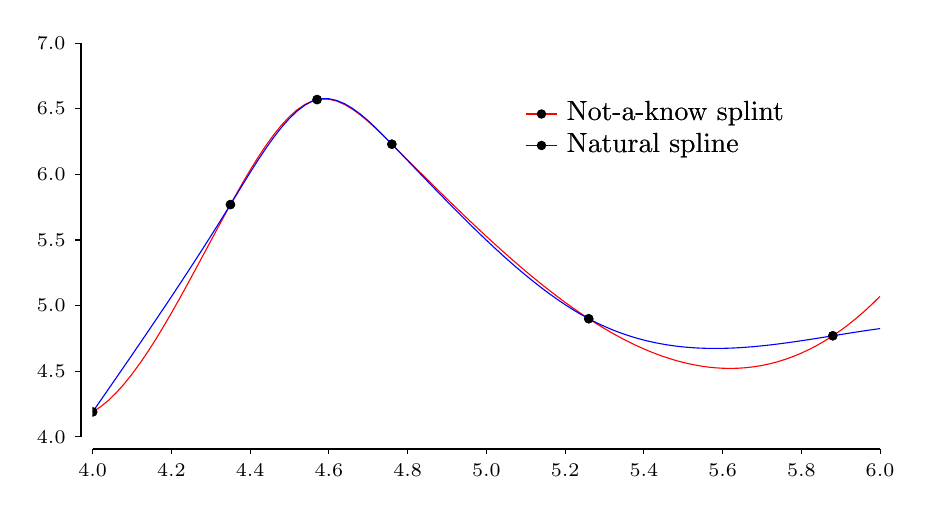
\begin{tikzpicture}[]
\begin{scope}[]
\pgfpathmoveto{ \pgfpointadd{\pgfpointxy {0.0} {0.0}} {\pgfpoint{0cm}{0cm}} }
\pgfpathlineto{ \pgfpointadd{\pgfpointxy {0.0} {0.0}} {\pgfpoint{10cm}{0cm}} }
\pgfpathlineto{ \pgfpointadd{\pgfpointxy {0.0} {0.0}} {\pgfpoint{10cm}{5cm}} }
\pgfpathlineto{ \pgfpointadd{\pgfpointxy {0.0} {0.0}} {\pgfpoint{0cm}{5cm}} }
\pgfpathclose
\pgfusepath{  clip, }
\begin{scope}[shift={(0.0,0.0)}]
\pgfsetxvec{\pgfpoint{5.0cm}{0cm}}
\pgfsetyvec{\pgfpoint{0cm}{1.6666666666666667cm}}
\begin{scope}[shift={(-4.0,-4.0)}]
\begin{scope}[]
\pgfpathmoveto{ \pgfpointadd{\pgfpointxy {4.0} {4.0}} {\pgfpoint{0cm}{0cm}} }
\pgfpathlineto{ \pgfpointadd{\pgfpointxy {4.0} {4.0}} {\pgfpoint{10cm}{0cm}} }
\pgfpathlineto{ \pgfpointadd{\pgfpointxy {4.0} {4.0}} {\pgfpoint{10cm}{5cm}} }
\pgfpathlineto{ \pgfpointadd{\pgfpointxy {4.0} {4.0}} {\pgfpoint{0cm}{5cm}} }
\pgfpathclose
\pgfusepath{  clip, }
\begin{scope}[red]
\pgfpathmoveto{ \pgfpointxy {4.0} {4.19}}
\pgfpathlineto{ \pgfpointxy {4.02} {4.2288933173496535}}
\pgfpathlineto{ \pgfpointxy {4.04} {4.277870024848159}}
\pgfpathlineto{ \pgfpointxy {4.06} {4.336184185327374}}
\pgfpathlineto{ \pgfpointxy {4.08} {4.403089861619165}}
\pgfpathlineto{ \pgfpointxy {4.1} {4.477841116555382}}
\pgfpathlineto{ \pgfpointxy {4.12} {4.559692012967896}}
\pgfpathlineto{ \pgfpointxy {4.14} {4.647896613688557}}
\pgfpathlineto{ \pgfpointxy {4.16} {4.741708981549234}}
\pgfpathlineto{ \pgfpointxy {4.18} {4.84038317938178}}
\pgfpathlineto{ \pgfpointxy {4.2} {4.943173270018062}}
\pgfpathlineto{ \pgfpointxy {4.22} {5.049333316289932}}
\pgfpathlineto{ \pgfpointxy {4.24} {5.158117381029259}}
\pgfpathlineto{ \pgfpointxy {4.26} {5.268779527067894}}
\pgfpathlineto{ \pgfpointxy {4.28} {5.380573817237705}}
\pgfpathlineto{ \pgfpointxy {4.3} {5.492754314370545}}
\pgfpathlineto{ \pgfpointxy {4.32} {5.604575081298282}}
\pgfpathlineto{ \pgfpointxy {4.34} {5.715290180852768}}
\pgfpathlineto{ \pgfpointxy {4.36} {5.824144492927248}}
\pgfpathlineto{ \pgfpointxy {4.38} {5.930171689826624}}
\pgfpathlineto{ \pgfpointxy {4.4} {6.032194236267487}}
\pgfpathlineto{ \pgfpointxy {4.42} {6.129025414027786}}
\pgfpathlineto{ \pgfpointxy {4.44} {6.2194785048854895}}
\pgfpathlineto{ \pgfpointxy {4.46} {6.302366790618549}}
\pgfpathlineto{ \pgfpointxy {4.48} {6.376503553004932}}
\pgfpathlineto{ \pgfpointxy {4.5} {6.440702073822589}}
\pgfpathlineto{ \pgfpointxy {4.52} {6.493775634849485}}
\pgfpathlineto{ \pgfpointxy {4.54} {6.53453751786358}}
\pgfpathlineto{ \pgfpointxy {4.5600000000000005} {6.56180100464283}}
\pgfpathlineto{ \pgfpointxy {4.58} {6.574437556572912}}
\pgfpathlineto{ \pgfpointxy {4.6} {6.572656766016991}}
\pgfpathlineto{ \pgfpointxy {4.62} {6.558006356315717}}
\pgfpathlineto{ \pgfpointxy {4.64} {6.532092230417464}}
\pgfpathlineto{ \pgfpointxy {4.66} {6.496520291270597}}
\pgfpathlineto{ \pgfpointxy {4.68} {6.452896441823487}}
\pgfpathlineto{ \pgfpointxy {4.7} {6.402826585024502}}
\pgfpathlineto{ \pgfpointxy {4.72} {6.347916623822015}}
\pgfpathlineto{ \pgfpointxy {4.74} {6.2897724611643895}}
\pgfpathlineto{ \pgfpointxy {4.76} {6.23}}
\pgfpathlineto{ \pgfpointxy {4.78} {6.169948902792082}}
\pgfpathlineto{ \pgfpointxy {4.8} {6.109943870063351}}
\pgfpathlineto{ \pgfpointxy {4.82} {6.050053361851389}}
\pgfpathlineto{ \pgfpointxy {4.84} {5.990345838193781}}
\pgfpathlineto{ \pgfpointxy {4.86} {5.9308897591281085}}
\pgfpathlineto{ \pgfpointxy {4.88} {5.871753584691959}}
\pgfpathlineto{ \pgfpointxy {4.9} {5.813005774922911}}
\pgfpathlineto{ \pgfpointxy {4.92} {5.754714789858553}}
\pgfpathlineto{ \pgfpointxy {4.94} {5.696949089536464}}
\pgfpathlineto{ \pgfpointxy {4.96} {5.639777133994231}}
\pgfpathlineto{ \pgfpointxy {4.98} {5.583267383269433}}
\pgfpathlineto{ \pgfpointxy {5.0} {5.5274882973996595}}
\pgfpathlineto{ \pgfpointxy {5.02} {5.47250833642249}}
\pgfpathlineto{ \pgfpointxy {5.04} {5.418395960375507}}
\pgfpathlineto{ \pgfpointxy {5.0600000000000005} {5.365219629296296}}
\pgfpathlineto{ \pgfpointxy {5.08} {5.3130478032224415}}
\pgfpathlineto{ \pgfpointxy {5.1} {5.261948942191526}}
\pgfpathlineto{ \pgfpointxy {5.12} {5.21199150624113}}
\pgfpathlineto{ \pgfpointxy {5.140000000000001} {5.1632439554088405}}
\pgfpathlineto{ \pgfpointxy {5.16} {5.115774749732242}}
\pgfpathlineto{ \pgfpointxy {5.18} {5.069652349248916}}
\pgfpathlineto{ \pgfpointxy {5.2} {5.0249452139964434}}
\pgfpathlineto{ \pgfpointxy {5.22} {4.9817218040124125}}
\pgfpathlineto{ \pgfpointxy {5.24} {4.940050579334401}}
\pgfpathlineto{ \pgfpointxy {5.26} {4.9}}
\pgfpathlineto{ \pgfpointxy {5.28} {4.861636317658478}}
\pgfpathlineto{ \pgfpointxy {5.3} {4.8250169504058755}}
\pgfpathlineto{ \pgfpointxy {5.32} {4.790197107949918}}
\pgfpathlineto{ \pgfpointxy {5.34} {4.757231999998338}}
\pgfpathlineto{ \pgfpointxy {5.36} {4.726176836258861}}
\pgfpathlineto{ \pgfpointxy {5.38} {4.697086826439219}}
\pgfpathlineto{ \pgfpointxy {5.4} {4.670017180247137}}
\pgfpathlineto{ \pgfpointxy {5.42} {4.645023107390346}}
\pgfpathlineto{ \pgfpointxy {5.4399999999999995} {4.622159817576572}}
\pgfpathlineto{ \pgfpointxy {5.46} {4.601482520513546}}
\pgfpathlineto{ \pgfpointxy {5.48} {4.583046425908996}}
\pgfpathlineto{ \pgfpointxy {5.5} {4.566906743470651}}
\pgfpathlineto{ \pgfpointxy {5.52} {4.55311868290624}}
\pgfpathlineto{ \pgfpointxy {5.54} {4.5417374539234885}}
\pgfpathlineto{ \pgfpointxy {5.5600000000000005} {4.532818266230128}}
\pgfpathlineto{ \pgfpointxy {5.58} {4.5264163295338875}}
\pgfpathlineto{ \pgfpointxy {5.6} {4.522586853542495}}
\pgfpathlineto{ \pgfpointxy {5.62} {4.521385047963677}}
\pgfpathlineto{ \pgfpointxy {5.640000000000001} {4.522866122505165}}
\pgfpathlineto{ \pgfpointxy {5.66} {4.527085286874686}}
\pgfpathlineto{ \pgfpointxy {5.68} {4.534097750779969}}
\pgfpathlineto{ \pgfpointxy {5.7} {4.543958723928742}}
\pgfpathlineto{ \pgfpointxy {5.72} {4.556723416028735}}
\pgfpathlineto{ \pgfpointxy {5.74} {4.572447036787675}}
\pgfpathlineto{ \pgfpointxy {5.76} {4.591184795913292}}
\pgfpathlineto{ \pgfpointxy {5.78} {4.612991903113314}}
\pgfpathlineto{ \pgfpointxy {5.8} {4.637923568095469}}
\pgfpathlineto{ \pgfpointxy {5.82} {4.666035000567487}}
\pgfpathlineto{ \pgfpointxy {5.84} {4.697381410237095}}
\pgfpathlineto{ \pgfpointxy {5.86} {4.732018006812025}}
\pgfpathlineto{ \pgfpointxy {5.88} {4.77}}
\pgfpathlineto{ \pgfpointxy {5.9} {4.811382599508753}}
\pgfpathlineto{ \pgfpointxy {5.92} {4.85622101504601}}
\pgfpathlineto{ \pgfpointxy {5.9399999999999995} {4.904570456319501}}
\pgfpathlineto{ \pgfpointxy {5.96} {4.9564861330369565}}
\pgfpathlineto{ \pgfpointxy {5.98} {5.0120232549061035}}
\pgfpathlineto{ \pgfpointxy {6.0} {5.071237031634667}}
\pgfusepath{ stroke, }
\end{scope}
\end{scope}
\begin{scope}[]
\pgfpathmoveto{ \pgfpointadd{\pgfpointxy {4.0} {4.0}} {\pgfpoint{0cm}{0cm}} }
\pgfpathlineto{ \pgfpointadd{\pgfpointxy {4.0} {4.0}} {\pgfpoint{10cm}{0cm}} }
\pgfpathlineto{ \pgfpointadd{\pgfpointxy {4.0} {4.0}} {\pgfpoint{10cm}{5cm}} }
\pgfpathlineto{ \pgfpointadd{\pgfpointxy {4.0} {4.0}} {\pgfpoint{0cm}{5cm}} }
\pgfpathclose
\pgfusepath{  clip, }
\node at (4.0,4.19) [fill=black,draw=black,circle,inner sep=0.0pt,minimum width =3.0pt,minimum height=3.0pt] {};
\node at (4.35,5.77) [fill=black,draw=black,circle,inner sep=0.0pt,minimum width =3.0pt,minimum height=3.0pt] {};
\node at (4.57,6.57) [fill=black,draw=black,circle,inner sep=0.0pt,minimum width =3.0pt,minimum height=3.0pt] {};
\node at (4.76,6.23) [fill=black,draw=black,circle,inner sep=0.0pt,minimum width =3.0pt,minimum height=3.0pt] {};
\node at (5.26,4.9) [fill=black,draw=black,circle,inner sep=0.0pt,minimum width =3.0pt,minimum height=3.0pt] {};
\node at (5.88,4.77) [fill=black,draw=black,circle,inner sep=0.0pt,minimum width =3.0pt,minimum height=3.0pt] {};
\end{scope}
\end{scope}
\end{scope}
\pgfsetxvec{\pgfpoint{1cm}{0cm}}
\pgfsetyvec{\pgfpoint{0cm}{1cm}}
\end{scope}
\draw[red] (5.5,4.1) -- (5.9,4.1);
\draw[opacity=0.0,white] (5.5,4.2) -- (5.5,4.0);
\node at (5.9,4.1) [right,] {Not-a-know splint};
\node at (5.7,4.1) [fill=black,draw=black,circle,inner sep=0.0pt,minimum width =3.0pt,minimum height=3.0pt] {};
\node at (5.9,4.1) [right,] {Not-a-know splint};
\begin{scope}[]
\pgfpathmoveto{ \pgfpointadd{\pgfpointxy {0.0} {0.0}} {\pgfpoint{0cm}{0cm}} }
\pgfpathlineto{ \pgfpointadd{\pgfpointxy {0.0} {0.0}} {\pgfpoint{10cm}{0cm}} }
\pgfpathlineto{ \pgfpointadd{\pgfpointxy {0.0} {0.0}} {\pgfpoint{10cm}{5cm}} }
\pgfpathlineto{ \pgfpointadd{\pgfpointxy {0.0} {0.0}} {\pgfpoint{0cm}{5cm}} }
\pgfpathclose
\pgfusepath{  clip, }
\begin{scope}[shift={(0.0,0.0)}]
\pgfsetxvec{\pgfpoint{5.0cm}{0cm}}
\pgfsetyvec{\pgfpoint{0cm}{1.6666666666666667cm}}
\begin{scope}[shift={(-4.0,-4.0)}]
\begin{scope}[]
\pgfpathmoveto{ \pgfpointadd{\pgfpointxy {4.0} {4.0}} {\pgfpoint{0cm}{0cm}} }
\pgfpathlineto{ \pgfpointadd{\pgfpointxy {4.0} {4.0}} {\pgfpoint{10cm}{0cm}} }
\pgfpathlineto{ \pgfpointadd{\pgfpointxy {4.0} {4.0}} {\pgfpoint{10cm}{5cm}} }
\pgfpathlineto{ \pgfpointadd{\pgfpointxy {4.0} {4.0}} {\pgfpoint{0cm}{5cm}} }
\pgfpathclose
\pgfusepath{  clip, }
\begin{scope}[blue]
\pgfpathmoveto{ \pgfpointxy {4.0} {4.19}}
\pgfpathlineto{ \pgfpointxy {4.02} {4.27659219042123}}
\pgfpathlineto{ \pgfpointxy {4.04} {4.363256980820145}}
\pgfpathlineto{ \pgfpointxy {4.06} {4.450066971174415}}
\pgfpathlineto{ \pgfpointxy {4.08} {4.537094761461732}}
\pgfpathlineto{ \pgfpointxy {4.1} {4.624412951659764}}
\pgfpathlineto{ \pgfpointxy {4.12} {4.712094141746202}}
\pgfpathlineto{ \pgfpointxy {4.14} {4.800210931698716}}
\pgfpathlineto{ \pgfpointxy {4.16} {4.888835921494997}}
\pgfpathlineto{ \pgfpointxy {4.18} {4.978041711112716}}
\pgfpathlineto{ \pgfpointxy {4.2} {5.067900900529561}}
\pgfpathlineto{ \pgfpointxy {4.22} {5.158486089723204}}
\pgfpathlineto{ \pgfpointxy {4.24} {5.249869878671334}}
\pgfpathlineto{ \pgfpointxy {4.26} {5.342124867351624}}
\pgfpathlineto{ \pgfpointxy {4.28} {5.43532365574176}}
\pgfpathlineto{ \pgfpointxy {4.3} {5.529538843819415}}
\pgfpathlineto{ \pgfpointxy {4.32} {5.624843031562279}}
\pgfpathlineto{ \pgfpointxy {4.34} {5.721308818948022}}
\pgfpathlineto{ \pgfpointxy {4.36} {5.818974279573464}}
\pgfpathlineto{ \pgfpointxy {4.38} {5.917083380275411}}
\pgfpathlineto{ \pgfpointxy {4.4} {6.014085981130691}}
\pgfpathlineto{ \pgfpointxy {4.42} {6.108397415835243}}
\pgfpathlineto{ \pgfpointxy {4.44} {6.198433018085027}}
\pgfpathlineto{ \pgfpointxy {4.46} {6.282608121575982}}
\pgfpathlineto{ \pgfpointxy {4.48} {6.359338060004066}}
\pgfpathlineto{ \pgfpointxy {4.5} {6.427038167065223}}
\pgfpathlineto{ \pgfpointxy {4.52} {6.484123776455401}}
\pgfpathlineto{ \pgfpointxy {4.54} {6.529010221870556}}
\pgfpathlineto{ \pgfpointxy {4.5600000000000005} {6.560112837006632}}
\pgfpathlineto{ \pgfpointxy {4.58} {6.575914836921859}}
\pgfpathlineto{ \pgfpointxy {4.6} {6.576460708006886}}
\pgfpathlineto{ \pgfpointxy {4.62} {6.563356207984786}}
\pgfpathlineto{ \pgfpointxy {4.64} {6.538274975940911}}
\pgfpathlineto{ \pgfpointxy {4.66} {6.502890650960607}}
\pgfpathlineto{ \pgfpointxy {4.68} {6.458876872129232}}
\pgfpathlineto{ \pgfpointxy {4.7} {6.4079072785321305}}
\pgfpathlineto{ \pgfpointxy {4.72} {6.351655509254659}}
\pgfpathlineto{ \pgfpointxy {4.74} {6.291795203382164}}
\pgfpathlineto{ \pgfpointxy {4.76} {6.23}}
\pgfpathlineto{ \pgfpointxy {4.78} {6.16768423115035}}
\pgfpathlineto{ \pgfpointxy {4.8} {6.105225000702742}}
\pgfpathlineto{ \pgfpointxy {4.82} {6.042740105483533}}
\pgfpathlineto{ \pgfpointxy {4.84} {5.98034734231909}}
\pgfpathlineto{ \pgfpointxy {4.86} {5.9181645080357645}}
\pgfpathlineto{ \pgfpointxy {4.88} {5.856309399459924}}
\pgfpathlineto{ \pgfpointxy {4.9} {5.794899813417925}}
\pgfpathlineto{ \pgfpointxy {4.92} {5.734053546736131}}
\pgfpathlineto{ \pgfpointxy {4.94} {5.6738883962408995}}
\pgfpathlineto{ \pgfpointxy {4.96} {5.614522158758593}}
\pgfpathlineto{ \pgfpointxy {4.98} {5.556072631115571}}
\pgfpathlineto{ \pgfpointxy {5.0} {5.498657610138196}}
\pgfpathlineto{ \pgfpointxy {5.02} {5.442394892652826}}
\pgfpathlineto{ \pgfpointxy {5.04} {5.387402275485819}}
\pgfpathlineto{ \pgfpointxy {5.0600000000000005} {5.333797555463539}}
\pgfpathlineto{ \pgfpointxy {5.08} {5.281698529412348}}
\pgfpathlineto{ \pgfpointxy {5.1} {5.231222994158605}}
\pgfpathlineto{ \pgfpointxy {5.12} {5.182488746528666}}
\pgfpathlineto{ \pgfpointxy {5.140000000000001} {5.1356135833488965}}
\pgfpathlineto{ \pgfpointxy {5.16} {5.090715301445657}}
\pgfpathlineto{ \pgfpointxy {5.18} {5.047911697645307}}
\pgfpathlineto{ \pgfpointxy {5.2} {5.007320568774205}}
\pgfpathlineto{ \pgfpointxy {5.22} {4.969059711658713}}
\pgfpathlineto{ \pgfpointxy {5.24} {4.93324692312519}}
\pgfpathlineto{ \pgfpointxy {5.26} {4.9}}
\pgfpathlineto{ \pgfpointxy {5.28} {4.869402678013522}}
\pgfpathlineto{ \pgfpointxy {5.3} {4.8414024485122304}}
\pgfpathlineto{ \pgfpointxy {5.32} {4.815912741746616}}
\pgfpathlineto{ \pgfpointxy {5.34} {4.792846987967176}}
\pgfpathlineto{ \pgfpointxy {5.36} {4.7721186174244}}
\pgfpathlineto{ \pgfpointxy {5.38} {4.753641060368786}}
\pgfpathlineto{ \pgfpointxy {5.4} {4.737327747050826}}
\pgfpathlineto{ \pgfpointxy {5.42} {4.723092107721014}}
\pgfpathlineto{ \pgfpointxy {5.4399999999999995} {4.710847572629844}}
\pgfpathlineto{ \pgfpointxy {5.46} {4.700507572027809}}
\pgfpathlineto{ \pgfpointxy {5.48} {4.691985536165404}}
\pgfpathlineto{ \pgfpointxy {5.5} {4.685194895293122}}
\pgfpathlineto{ \pgfpointxy {5.52} {4.680049079661458}}
\pgfpathlineto{ \pgfpointxy {5.54} {4.676461519520904}}
\pgfpathlineto{ \pgfpointxy {5.5600000000000005} {4.674345645121956}}
\pgfpathlineto{ \pgfpointxy {5.58} {4.6736148867151055}}
\pgfpathlineto{ \pgfpointxy {5.6} {4.674182674550848}}
\pgfpathlineto{ \pgfpointxy {5.62} {4.675962438879676}}
\pgfpathlineto{ \pgfpointxy {5.640000000000001} {4.678867609952086}}
\pgfpathlineto{ \pgfpointxy {5.66} {4.682811618018568}}
\pgfpathlineto{ \pgfpointxy {5.68} {4.687707893329618}}
\pgfpathlineto{ \pgfpointxy {5.7} {4.693469866135731}}
\pgfpathlineto{ \pgfpointxy {5.72} {4.700010966687398}}
\pgfpathlineto{ \pgfpointxy {5.74} {4.707244625235115}}
\pgfpathlineto{ \pgfpointxy {5.76} {4.715084272029376}}
\pgfpathlineto{ \pgfpointxy {5.78} {4.723443337320674}}
\pgfpathlineto{ \pgfpointxy {5.8} {4.732235251359502}}
\pgfpathlineto{ \pgfpointxy {5.82} {4.741373444396355}}
\pgfpathlineto{ \pgfpointxy {5.84} {4.750771346681726}}
\pgfpathlineto{ \pgfpointxy {5.86} {4.7603423884661105}}
\pgfpathlineto{ \pgfpointxy {5.88} {4.77}}
\pgfpathlineto{ \pgfpointxy {5.9} {4.77965761153389}}
\pgfpathlineto{ \pgfpointxy {5.92} {4.789228653318274}}
\pgfpathlineto{ \pgfpointxy {5.9399999999999995} {4.7986265556036445}}
\pgfpathlineto{ \pgfpointxy {5.96} {4.807764748640497}}
\pgfpathlineto{ \pgfpointxy {5.98} {4.816556662679326}}
\pgfpathlineto{ \pgfpointxy {6.0} {4.824915727970623}}
\pgfusepath{ stroke, }
\end{scope}
\end{scope}
\begin{scope}[]
\pgfpathmoveto{ \pgfpointadd{\pgfpointxy {4.0} {4.0}} {\pgfpoint{0cm}{0cm}} }
\pgfpathlineto{ \pgfpointadd{\pgfpointxy {4.0} {4.0}} {\pgfpoint{10cm}{0cm}} }
\pgfpathlineto{ \pgfpointadd{\pgfpointxy {4.0} {4.0}} {\pgfpoint{10cm}{5cm}} }
\pgfpathlineto{ \pgfpointadd{\pgfpointxy {4.0} {4.0}} {\pgfpoint{0cm}{5cm}} }
\pgfpathclose
\pgfusepath{  clip, }
\node at (4.0,4.19) [fill=black,draw=black,circle,inner sep=0.0pt,minimum width =3.0pt,minimum height=3.0pt] {};
\node at (4.35,5.77) [fill=black,draw=black,circle,inner sep=0.0pt,minimum width =3.0pt,minimum height=3.0pt] {};
\node at (4.57,6.57) [fill=black,draw=black,circle,inner sep=0.0pt,minimum width =3.0pt,minimum height=3.0pt] {};
\node at (4.76,6.23) [fill=black,draw=black,circle,inner sep=0.0pt,minimum width =3.0pt,minimum height=3.0pt] {};
\node at (5.26,4.9) [fill=black,draw=black,circle,inner sep=0.0pt,minimum width =3.0pt,minimum height=3.0pt] {};
\node at (5.88,4.77) [fill=black,draw=black,circle,inner sep=0.0pt,minimum width =3.0pt,minimum height=3.0pt] {};
\end{scope}
\end{scope}
\end{scope}
\pgfsetxvec{\pgfpoint{1cm}{0cm}}
\pgfsetyvec{\pgfpoint{0cm}{1cm}}
\end{scope}
\draw[blue] (5.5,3.7) -- (5.9,3.7);
\draw[opacity=0.0,white] (5.5,3.8000000000000003) -- (5.5,3.6);
\node at (5.9,3.7) [right,] {Natural spline};
\node at (5.7,3.7) [fill=black,draw=black,circle,inner sep=0.0pt,minimum width =3.0pt,minimum height=3.0pt] {};
\node at (5.9,3.7) [right,] {Natural spline};
\begin{scope}[shift={(0.0,0.0)}]
\pgfsetxvec{\pgfpoint{5.0cm}{0cm}}
\pgfsetyvec{\pgfpoint{0cm}{1.6666666666666667cm}}
\begin{scope}[shift={(-4.0,-4.0)}]
\begin{scope}[thick,black,fill=white]
\pgfpathmoveto{ \pgfpointadd{\pgfpointxy {4.0} {4.0}} {\pgfpoint{0}{-0.15cm}} }
\pgfpathlineto{ \pgfpointadd{\pgfpointxy {6.0} {4.0}} {\pgfpoint{0}{-0.15cm}} }
\pgfpathmoveto{ \pgfpointadd{\pgfpointxy {4.0} {4.0}} {\pgfpoint{-0.15cm}{0}} }
\pgfpathlineto{ \pgfpointadd{\pgfpointxy {4.0} {7.0}} {\pgfpoint{-0.15cm}{0}} }
\pgfusepath{ stroke, }
\end{scope}
\begin{scope}[yshift=-0.15cm]
\draw[] [shift={(4.0,4.0)}] (0,0) -- (0,-2pt) node[below]{ \scriptsize{\num[round-mode=places,round-precision=1]{4.0}}};
\draw[] [shift={(4.2,4.0)}] (0,0) -- (0,-2pt) node[below]{ \scriptsize{\num[round-mode=places,round-precision=1]{4.2}}};
\draw[] [shift={(4.4,4.0)}] (0,0) -- (0,-2pt) node[below]{ \scriptsize{\num[round-mode=places,round-precision=1]{4.4}}};
\draw[] [shift={(4.6,4.0)}] (0,0) -- (0,-2pt) node[below]{ \scriptsize{\num[round-mode=places,round-precision=1]{4.6}}};
\draw[] [shift={(4.8,4.0)}] (0,0) -- (0,-2pt) node[below]{ \scriptsize{\num[round-mode=places,round-precision=1]{4.8}}};
\draw[] [shift={(5.0,4.0)}] (0,0) -- (0,-2pt) node[below]{ \scriptsize{\num[round-mode=places,round-precision=1]{5.0}}};
\draw[] [shift={(5.2,4.0)}] (0,0) -- (0,-2pt) node[below]{ \scriptsize{\num[round-mode=places,round-precision=1]{5.2}}};
\draw[] [shift={(5.4,4.0)}] (0,0) -- (0,-2pt) node[below]{ \scriptsize{\num[round-mode=places,round-precision=1]{5.4}}};
\draw[] [shift={(5.6,4.0)}] (0,0) -- (0,-2pt) node[below]{ \scriptsize{\num[round-mode=places,round-precision=1]{5.6}}};
\draw[] [shift={(5.8,4.0)}] (0,0) -- (0,-2pt) node[below]{ \scriptsize{\num[round-mode=places,round-precision=1]{5.8}}};
\draw[] [shift={(6.0,4.0)}] (0,0) -- (0,-2pt) node[below]{ \scriptsize{\num[round-mode=places,round-precision=1]{6.0}}};
\end{scope}
\begin{scope}[xshift=-0.15cm]
\draw[] [shift={(4.0,4.0)}] (0,0) -- (-2pt,0) node[left]{ \scriptsize{\num[round-mode=places,round-precision=1]{4.0}}};
\draw[] [shift={(4.0,4.5)}] (0,0) -- (-2pt,0) node[left]{ \scriptsize{\num[round-mode=places,round-precision=1]{4.5}}};
\draw[] [shift={(4.0,5.0)}] (0,0) -- (-2pt,0) node[left]{ \scriptsize{\num[round-mode=places,round-precision=1]{5.0}}};
\draw[] [shift={(4.0,5.5)}] (0,0) -- (-2pt,0) node[left]{ \scriptsize{\num[round-mode=places,round-precision=1]{5.5}}};
\draw[] [shift={(4.0,6.0)}] (0,0) -- (-2pt,0) node[left]{ \scriptsize{\num[round-mode=places,round-precision=1]{6.0}}};
\draw[] [shift={(4.0,6.5)}] (0,0) -- (-2pt,0) node[left]{ \scriptsize{\num[round-mode=places,round-precision=1]{6.5}}};
\draw[] [shift={(4.0,7.0)}] (0,0) -- (-2pt,0) node[left]{ \scriptsize{\num[round-mode=places,round-precision=1]{7.0}}};
\end{scope}
\end{scope}
\end{scope}
\pgfsetxvec{\pgfpoint{1cm}{0cm}}
\pgfsetyvec{\pgfpoint{0cm}{1cm}}
\end{tikzpicture}
\end{document}


\end{document}


  
%%% Local Variables: 
%%% mode: latex
%%% TeX-master: t
%%% End: 
